% % Konfiguration für Texstudio (Version > 2.9)
% !TeX program = xelatex
% !TeX TXS-program:compile = txs:///xelatex/[-8bit]
% !BIB program = biber
% !TeX spellcheck = en_US
% !TeX encoding = utf8

% Copyright 2018-2023 by Romano Giannetti
% Copyright 2015-2023 by Stefan Lindner
% Copyright 2013-2023 by Stefan Erhardt
% Copyright 2007-2023 by Massimo Redaelli
%
% This file may be distributed and/or modified
%
% 1. under the LaTeX Project Public License and/or
% 2. under the GNU Public License.
%
% See the files gpl-3.0_license.txt and lppl-1-3c_license.txt for more details.
%

\documentclass[a4paper, titlepage]{article}

\def\modern{
	\usepackage{fontspec}
	\defaultfontfeatures{
      Ligatures=TeX,
      Numbers=OldStyle,
      Mapping=tex-text,
      SmallCapsFeatures={LetterSpace=8, Numbers=OldStyle}
	}
	% \setmainfont{Gentium Book Basic}
}

% do not split this line in more lines, otherwise "make git-manual" will show the wrong version
\usepackage[siunitx, RPvoltages]{circuitikz}
% Let this be the same as the chosen voltage direction for coherence
\def\chosenvoltoption{RPvoltages}
%
\usepackage{ifxetex,ifluatex}
\ifxetex
	\modern
\else
	\ifluatex
		\modern
	\else
	% pdflatex
		\usepackage[T1]{fontenc}
		\usepackage[utf8]{inputenc}
        \usepackage{lmodern}
		% \usepackage{babel}
	\fi
\fi
\def\tightlist{} % needed for latest pandoc-versions(pandoc used for including changelog)
\usepackage{microtype}

\usepackage{imakeidx}
\makeindex[title=Index of the components, intoc=true]

% Local utilities packages
\usepackage{ctikzmanutils}
%

\begin{document}
% change numbering to roman to avoid a duplicate hyperref target on page 1
% Thanks to Ulrike Fischer for helping here
\pagenumbering{roman}
\title{\Circuitikz \\{\large version \pgfcircversion{} (\pgfcircversiondate)}}
\author{Massimo A. Redaelli (\email{m.redaelli@gmail.com})\\
    Stefan Lindner (\email{stefan.lindner@fau.de})\\
    Stefan Erhardt (\email{stefan.erhardt@fau.de})\\
    Romano Giannetti (\email{romano.giannetti@gmail.com})}
\date{\today}

\pretitle{\begin{center}%
    \begin{circuitikz}
        \draw (0,0) node[dipchip, rotate=90, num pins=40, fill=cyan!20!white](C){%
            \rotatebox{-90}{\LARGE\Circuitikz}%
        };
        \draw (C.pin 20) -- ++(0,-8) node[ground](GND){};
        \draw (C.pin 7) to[D, fill=blue] ++(0,-1) -- ++(0.5,0) to[R] ++(2,0)
            coordinate(a1) to[short, -*]
            node[above left, blue, pos=1]{Massimo A. Redaelli}
            node[below left, pos=1]{\email{m.redaelli@gmail.com}}
            (a1-|GND);
            \draw (C.pin 5) to[D, fill=red] ++(0,-3)-- ++(0.5,0) to[R] ++(2,0)
            coordinate(a2) to[short, -*]
            node[above left, blue, pos=1]{Stefan Lindner}
            node[below left, pos=1]{\email{stefan.lindner@fau.de}}
            (a2-|GND);
            \draw (C.pin 3) to[D, fill=green] ++(0,-5)-- ++(0.5,0) to[R] ++(2,0)
            coordinate(a3) to[short, -*]
            node[above left, blue, pos=1]{Stefan Erhardt}
            node[below left, pos=1]{\email{stefan.erhardt@fau.de}}
            (a3-|GND);
            \draw (C.pin 1) to[D, fill=yellow] ++(0,-7)-- ++(0.5,0) to[R] ++(2,0)
            coordinate(a4) to[short, -*]
            node[above left, blue, pos=1]{Romano Giannetti}
            node[below left, pos=1]{\email{romano.giannetti@gmail.com}}
            (a4-|GND);
    \end{circuitikz}
    \par\bigskip\vfill}
\posttitle{\end{center}}

\maketitle

% go back to arabic numbering after the titlepage
\pagenumbering{arabic}
\tableofcontents

\section{Introduction}

\hfill\begin{minipage}[t]{0.5\textwidth}
    \small\slshape\raggedleft
    Lorenzo and Mirella, 57 years ago, started a trip that eventually lead to a lot of things --- among them, \Circuitikz{} \texttt{v1.0}.

    In loving memory
    --- R.\@G.\@, 2020-02-04
\end{minipage}

\subsection{About}
\Circuitikz{} was initiated by Massimo Redaelli in 2007, who was working as a research assistant at the Polytechnic University of Milan, Italy, and needed a tool for creating exercises and exams.
After he left University in 2010 the development of \Circuitikz\ slowed down, since \LaTeX\ is mainly established in the academic world. In 2015 Stefan Lindner and Stefan Erhardt, both working as research assistants at the University of Erlangen-Nürnberg, Germany, joined the team and now maintain the project together with the initial author. In 2018 Romano Giannetti, full professor of Electronics at Comillas Pontifical University of Madrid, joined the team.

The use of \Circuitikz\ is, of course, not limited to academic teaching. The package gets widely used by engineers for typesetting electronic circuits for articles and publications all over the world.

\subsection{License}
Copyright \copyright{}
2007--2023 by Massimo Redaelli,
2013--2023 by Stefan Erhardt,
2015--2023 by Stefan Lindner,
and 2018--2023 by Romano Giannetti.
This package is author-maintained. Permission is granted to copy, distribute and/or modify this software under the terms of the \LaTeX\ Project Public License, version 1.3.1, or the GNU Public License. This software is provided ‘as is’, without warranty of any kind, either expressed or implied, including, but not limited to, the implied warranties of merchantability and fitness for a particular purpose.
\subsection{Loading the package}

\begin{table}[h]
\centering
\begin{tabular}{ll}\toprule
	\LaTeX       	& \ConTeXt\footnotemark \\ \midrule
	\verb!\usepackage{circuitikz}!	& \verb!\usemodule[circuitikz]!\\
	\bottomrule
\end{tabular}
\end{table}
\footnotetext{\ConTeXt\ support was added mostly thanks to Mojca Miklavec and Aditya Mahajan.\textbf{Please notice} that since \ConTeXt{} switched to the new \texttt{lmtx} engine (March 2023), there can be problems to compile \TikZ{} which some version; in May 2023 the problem has been fixed. Please check \href{https://github.com/circuitikz/circuitikz/issues/706}{this issue} for details.}


\noindent \TikZ\ will be automatically loaded; additionally, the \TikZ{} libraries \texttt{calc}, \texttt{arrows.meta}, \texttt{bending}, and \texttt{fpu} are loaded (the last one is used only on demand).

\noindent Circui\TikZ\ commands are just \TikZ\ commands, so a minimum usage example would be:

\begin{LTXexample}[varwidth=true]
\tikz \draw (0,0) to[R=$R_1$] (2,0);
\end{LTXexample}

There is really no support for Plain TeX --- the maintainers are willing to consider patches if somebody is interested.

\subsection{Installing a new version of the package.}

The stable version of the package should come with your \LaTeX\ distribution. Downloading the files from CTAN and installing them locally is, unfortunately, a distribution-dependent task and sometimes not so trivial. If you search for \texttt{local texmf tree} and the name of your distribution on \url{https://tex.stackexchange.com/} you will find a lot of hints.

Anyway, the easiest way of using whichever version of \Circuitikz\ is to point to the GitHub page \url{https://circuitikz.github.io/circuitikz/} of the project, and download the version you want. You will download a simple (biggish) file, called \texttt{circuitikzgit.sty}.

Now you can just put this file in your local \texttt{texmf} tree, if you have one, or simply adding it into the same directory where your main file resides, and then use

\begin{verbatim}
    \usepackage[...options...]{circuitikzgit}
\end{verbatim}

instead of \texttt{circuitikz}. This is also advantageous for ``future resilience''; the authors try hard not to break backward compatibility with new versions, but sometimes, things happen.

\subsection{Requirements}
\begin{itemize}
    \item \texttt{tikz}, version ${}\ge{}$\texttt{3.1.5b} (it \emph{should} work with any version from 3.0 and up, but better use a newer one);
    \item \texttt{xstring}, not older than 2009/03/13;
    \item \texttt{siunitx}, if using \texttt{siunitx} option (better \texttt{v2} or newer).
\end{itemize}

A similar approach for \ConTeXt\ is available, with the file \texttt{t-circuitikzgit.tex}; the compatibility in this case is not guaranteed, but provided on a \emph{best effort} base.

This manual has been typeset with \Circuitikz{} \pgfcircversion{} (\pgfcircversiondate) on \TikZ{} \pgfversion{} (\pgfversiondate).

\subsection{Incompatible packages}\label{sec:incompatible-packages}

\TikZ's own \texttt{circuit} library, which was based on \Circuitikz, (re?)defines several styles used by this library. In order to have them work together you can use the \texttt{compatibility} package option, which basically prefixes the names of all \Circuitikz\ \texttt{to[]} styles with an asterisk.

So, if loaded with said option, one must write \verb!(0,0) to[*R] (2,0)! and, for transistors on a path, \verb!(0,0) to[*Tnmos] (2,0)!, and so on (but \verb!(0,0) node[nmos] {}!). See example at page~\pageref{ex:compatibility}.

Anyway, the compatibility code is a \emph{best effort} task and only very lightly tested --- the authors advice is to choose one or the other,  without mixing them.

Another thing to take into account is that any \TikZ{} figure (and \Circuitikz{} ones qualify) \textbf{will} have problems if you use the \texttt{babel} package with a language that changes active characters (most of them). The solution is normally to add the line \verb|\usetikzlibrary{babel}| in your preamble, after loading \TikZ{} or \Circuitikz. This will normally solve the problem; some languages also require using \verb|\deactivatequoting| or the option \texttt{shorthands=off} for \texttt{babel}. Please check the documentation of \TikZ{} or this question \href{https://tex.stackexchange.com/questions/166772/problem-with-babel-and-tikz-using-draw}{on \TeX{} stackexchange site}.

Finally, the \TikZ{} library \texttt{bending} is loaded by the package, and its effects (the bending of the arrows on curved paths) will also affect the rest of your drawings.

\subsection{Known bugs and limitation}\label{sec:bugs}

\Circuitikz{} will \textbf{not work} correctly with global (in the main \texttt{circuitikz} environment, or in \texttt{scope} environments) \emph{negative} scale parameters (\texttt{scale}, \texttt{xscale} or \texttt{yscale}), unless \texttt{transform shape} is also used, and even in this cases the behavior is not guaranteed.
Neither will it work with angle-changing scaling (when \texttt{xscale} is different form \texttt{yscale}) and with the global \texttt{rotate} parameter.

Correcting this will need a big rewrite of the path routines, and although the authors are thinking about solving it, don't hold your breath; it will need changing a lot of interwoven code (labels, voltages, currents and so on). Contributions and help would be highly appreciated.

This same issue creates a lot of problems with compatibility between \Circuitikz{} and the new \texttt{pic} \TikZ\  feature, so basically don't put components into \texttt{pic}s.

Also, notice that several components will interact in a funny way with global path options. Depending on the specific component, some parameters are inherited by the internal shape, and some others are reset. This is not easy to fix in general. We want some options to go through --- fill color, dashed pattern for example --- and some others to stay only in the outer path; and if the background shape needs some option for drawing the internal shape, like for example a rounded corner, it \emph{must} reset the external option. So there is no perfect solution, although since \texttt{v1.5.0} the shapes have been ``robustified'', so that by default arced corners and arrows parameters will \emph{not} be propagated into the shape.
Arrows with \texttt{to[]} components don't work, anyway, so basically avoid this situation.

\begin{LTXexample}[varwidth=true, basicstyle=\small\ttfamily]
\begin{circuitikz}[]
    \draw (0,3) to[R] ++(3,0) node[npn, anchor=B]{};
    % arrows will not work and give strange results
    % so basically do not use them!
    \draw[<->] (0,1.5) to[R] ++(3,0) node[npn, anchor=B]{};
    \draw[shorten <=10pt] (0,0) to[R] ++(3,0)
         node[npn, anchor=B]{};
\end{circuitikz}
\end{LTXexample}

Lastly, voltage styles interacts in strange ways with general (such as \texttt{american}, \texttt{european} style), in the sense that sometimes the order in which you enact them is important. That should be arguably fixed, but it will change (read break) a lot of existing code, so it'll stay;  more information and workarounds in section~\ref{sec:mixing-voltage-styles}.

As a final notice, if you want to use the \texttt{externalize} library, do not use the \texttt{circuitikz} environment: use \texttt{tikzpicture} (which is really the same thing, see the FAQ~\ref{faqs:externalize}).

\subsection{Scale factor inaccuracies}\label{sec:usefpu}

Sometimes, when using fractional scaling factors and big values for the coordinates, the basic layer inaccuracies from \TeX{} can bite you, producing results like the following one:

\begin{LTXexample}[varwidth=true]
\begin{circuitikz}[scale=1.2, transform shape,
    ]
    \draw (60,1) to [battery2, v_=$V_{cc}$, name=B] ++(0,2);
    \node[draw,red,circle,inner sep=4pt] at(B.left) {};
    \node[draw,red,circle,inner sep=4pt] at(B.right) {};
\end{circuitikz}
\end{LTXexample}

A general solution for this problem is difficult to find; probably the best approach is to use a \verb|scalebox| command to scale the circuit instead of relying on internal scaling.

Nevertheless,  \href{https://tex.stackexchange.com/a/529159/38080}{Schrödinger's cat} found a solution which has been ported to \Circuitikz: you can use the  key \texttt{use fpu reciprocal} which will patch a standard low-level math routine with a more precise one.

\begin{LTXexample}[varwidth=true]
\begin{circuitikz}[scale=1.2, transform shape,
    use fpu reciprocal,
    ]
\draw (60,1) to [battery2, v_=$V_{cc}$] ++(0,2);
\end{circuitikz}
\end{LTXexample}

The \texttt{use fpu reciprocal} key seems to have no side effects, but given that it is patching an internal interface of \TikZ{} it can break any time, so it is advisable to use it only if and when needed.


\subsection{Incompabilities between versions}\label{sec:incompatible-changes}
Here, we will provide a list of incompatibilities between different versions of \Circuitikz. We will try to hold this list short, but sometimes it is easier to break with old syntax than include a lot of switches and compatibility layers. In general, changes that would invalidate a circuit (changes of polarity of components and so on) are almost always protected by a flag; the same is not true for purely aesthetic changes.
If unsure, you can check the version in your local installation by using the macro \verb!\pgfcircversion{}!.
\begin{itemize}
    \item Since version \texttt{1.6.3} the default symbol for the minus sign changed from the simple \verb|$-$| to \verb|$\vphantom{+}-$|. The reason is that in some (most?) font, the minus sign is enclosed in a smaller bounding box than the plus sign and that leads to poorly aligned minus symbols in \texttt{american} and \texttt{raised} voltages. This was not noticed before because the two symbols share the same bounding box in the default Computer Modern font. You can look at \href{https://github.com/circuitikz/circuitikz/issues/721}{this issue on GitHub} for more details; if you want to go back to the previous definitions you can write
        \begin{lstlisting}
            \ctikzset{amplifiers/minus=$-$}
            \ctikzset{bipoles/cvsourceam/inner minus=$-$}
            \ctikzset{bipoles/vsourceam/inner minus=$-$}
            \ctikzset{voltage/american minus=$-$}
        \end{lstlisting}
    \item Since version \texttt{1.6.3} the size of the solder dot and the connection dot of the body diodes for transistors has changed (now they are the same and are configurable). The new default scale of~\texttt{0.7} makes the dots \emph{area} more or less one half the one of the external connections. You can go back to the previous values with
        \begin{lstlisting}
            \ctikzset{transistor bodydiode/dot scale=0.5,
                transistor solderdot scale=1.0}
        \end{lstlisting}
    \item Since version \texttt{1.6.2} \texttt{siunitx}  will \textbf{not}  work anymore with \ConTeXt{} (it was a very poor simulation layer, anyway); it has been disabled in upstream \ConTeXt, in favor of \href{https://www.pragma-ade.nl/general/manuals/units-mkiv.pdf}{its own \texttt{units} module}.
    \item Version \texttt{1.6.0} has a big rewrite of the block's code. In principle the changes are backward-compatible, but there were several bugs (wrong anchors, errors with rotations, and so on) that have been fixed in the process.
    \item Since \texttt{v1.5.1}\footnote{Do not use \texttt{v1.5.0}, it's buggy.} color management (see section~\ref{sec:colors}) and the details of how the shapes are drawn and protected by the external drawing options has changed. There should be no substantial changes to the circuits, though.
    \item The \TikZ{} fix for \texttt{to[...] +(x,y)} behavior (see~\ref{sec:path-relative-coordinates}) uncovered a bug in the positioning of the labels in \Circuitikz{} that had been present since \texttt{v0.8}. So you \textbf{must} upgrade to \texttt{v1.4.1} or better if you have \TikZ{} newer than \texttt{3.1.8} (and you want/need to use the \texttt{+(x,y)} syntax).
    \item There have been changes in (internal) parameters for capacitors in \texttt{v1.4.1}; now to change them you should use the style interface (see~\ref{sec:capacitors-styling}).
    \item \Circuitikz{} \texttt{v1.4.0} introduced the rollback system for the package when using LaTeX; that (at least in principle) should be completely backward-compatible.
    \item The path construction in \texttt{v1.4.0} has been changed a bit (again). The change shouldn't break any circuit and will correct a behavior that should have been fixed with the \texttt{v1.2.1} change (see below).
    \item Version 1.3.6 fixes several problems with the stacked labels; the most important change is that now the bracing of arguments is respected as in version 1.3.0 for the other labels. The special treatment in stacked labels (and only in stacked labels!) for the (still experimental\footnote{and, really, not advised\dots}) \texttt{siunitx} compact syntax \texttt{<...>} has been removed: it was completely buggy before, and silently ignored, now will throw an error.
    \item Version 1.3.3 fixes the direction of the arrows in tunable elements; before this version, they were more or less random, now the arrow goes from bottom left to top right. You have the option to go back to the old behavior with \texttt{\textbackslash ctikzset\{bipoles/fix tunable direction=false\}}. As a compensation for the fuss, now the arrows are configurable. To learn more, see the FAQ:~\ref{faq:tunable-arrow}.
    \item Version 1.3.1 removes the warning if you do not specify a voltage direction.
    \item Version 1.3.0 fixes the buggy stripping of braces from labels and annotations (see~\ref{sec:bracing-of-labels}).
    \item After 1.2.7 a big code reorganization (which had the collateral effect of fixing some bugs) has been made; no changes should be visible, but a fallback point at 1.2.7 has been added.
    \item You \textbf{must} upgrade to v1.2.7 or newer if you use a \TikZ{} 3.1.8 or 3.1.8a (but better upgrade both packages to the current version). You can check the \TikZ{} version installed using the macro \verb|\pgfversion|.
    \item After v1.2.1: \textbf{Important:} the routine that implements the \texttt{to[...]} component positioning has been rewritten. That should enhance the line joins in paths, and it's safer, but it can potentially change some old behavior.

        One of the changes is that the previous routine did the wrong thing if you used \texttt{(node) to[...]} (you should use an anchor or a coordinate, not a node there --- like \texttt{(node.anchor) to[...]}).

        The other one was that in the structure \texttt{... to[...] node[pos=\emph{something}]  (coord)} the value of \texttt{pos} was completely wrong (even if you don't use \texttt{pos} explicitly, remember it's \texttt{pos=0.5} by default).

        Additionally, the old code disrupted the \TikZ{} path-fill mechanism, so that you could get away with using the \texttt{fill} option on paths and having just the components filled, not the path. That was incorrect, although sometime it was handy (sorry).

        See the FAQ at section~\ref{faqs:nodes} for more information.

    \item After v1.2.0: voltage arrows, symbols and label positions are calculated with a rewritten routine. There should be little change, \emph{unless} you touched internal values\dots
    \item After v1.1.3: from version 1.1.0 to version 1.1.2, the inverted Schmitt buffer in IEEE style ports was called \texttt{inv schmitt} (with an additional space). The correct name is \texttt{invschmitt port} (the same as the legacy american port).
    \item After v1.1.2: the position of \texttt{american} voltages for the \texttt{open} bipoles changed (you can revert to the old behavior, see section~\ref{sec:sub-voltage-position}).
    \item After v0.9.7: the position of the text of transistor nodes has changed; see section~\ref{sec:transistors-labels}.
    \item After v0.9.4: added the concept of styling of circuits. It should be backward compatible, but it's a big change, so be ready to use the \texttt{0.9.3} snapshot (see below for details).
    \item After v0.9.0: the parameters \texttt{tripoles/american or port/aaa}, \texttt{...bbb}, \texttt{...ccc} and \texttt{...ddd} are no longer used and are silently ignored; the same stands for the similarly named parameters in \texttt{nor}, \texttt{xor}, and \texttt{xnor} ports.
    \item After v0.9.0: voltage and current directions/signs (plus and minus signs in case of \texttt{american voltages} and arrows in case of \texttt{european voltages}) have been rationalized with a couple of new options (see details in section~\ref{curr-and-volt}). The default case is still the same as v0.8.3, to avoid potentially wrong circuits, but you would be better off with one of the new voltage directions (\texttt{EFvoltages} or \texttt{RPvoltages}) for newer circuits.
    \item Since v0.8.2: voltage and current label directions (\texttt{v<=} / \texttt{i<=}) do NOT change the orientation of the drawn source shape anymore. Use the \texttt{invert} option to rotate the shape of the source. Furthermore, from this version on, the current label (\texttt{i=}) at current sources can be used independent of the regular label (\texttt{l=}).
    \item Since v0.7: The label behavior at mirrored bipoles has changed, this fixes the voltage drawing, but perhaps you will have to adjust your label positions.
    \item Since v0.5.1: The parts \texttt{pfet}, \texttt{pigfete}, \texttt{pigfetebulk}, and \texttt{pigfetd} are now mirrored by default. Please adjust your yscale-option to correct this.
    \item Since v0.5: New voltage counting direction, there exists an option to use the old behavior.
\end{itemize}

If you have older projects that show compatibility problems, you have two options:
\begin{itemize}
    \item you can use an older version locally using the git-version and picking the correct commit from the repository (branch gh-pages) or the main GitHub site directly;
    \item if you are using \LaTeX, the distribution has embedded several important old versions: \texttt{0.4}, \texttt{0.6}, \texttt{0.7}, \texttt{0.8.3}, \texttt{0.9.3}, \texttt{0.9.6}, \texttt{1.0}, \texttt{1.1.2}, \texttt{1.2.7}, and \texttt{1.4.6}.
        To switch to use them, since \texttt{v1.4.0} you simply use the \href{https://www.latex-project.org/publications/2018-FMi-TUB-tb122mitt-version-rollback.pdf}{new LaTeX kernel rollback system}, changing your \verb|\usepackage| invocation to something like:
        \begin{lstlisting}[numbers=none]
            \usepackage[]{circuitikz}[=v0.8.3] % or v0.4, v0.6, ...
        \end{lstlisting}
        You can also specify a date instead of a version number: if you write
        \begin{lstlisting}[numbers=none]
            \usepackage[]{circuitikz}[=2020/02/05]
        \end{lstlisting}
        the rollback system will load the version that was current on February 5th,~2020 (in this case it will be \texttt{v1.0} which was released the day before).

        If for whatever reasons your kernel is older, you can still use the old method of loading the \emph{package-version} package; for example:
        \begin{lstlisting}[numbers=none]
            \usepackage[]{circuitikz-0.8.3} % or circuitikz-0.4, 0.6...
        \end{lstlisting}
        which is an inferior solution because it can fool any package you use that depend on \texttt{circuitikz}.

        Either way, you have to take care of the options that may have changed between versions (and sometime styles, if you use them).
    \item   if you are using  \ConTeXt, only versions \texttt{0.8.3}, \texttt{0.9.3},  \texttt{0.9.6}, \texttt{1.0}, \texttt{1.1.2}, \texttt{1.2.7}, and \texttt{1.4.6} are packaged; you can use it with
        \begin{lstlisting}[numbers=none]
            \usemodule[circuitikz-0.8.3]
        \end{lstlisting}
\end{itemize}


\subsection{Feedback}
The easiest way to contact the authors is via the official GitHub repository: \url{https://github.com/circuitikz/circuitikz/issues}. For general help question, a lot of nice people are  quite active on \url{https://tex.stackexchange.com/questions/tagged/circuitikz} --- be sure to read the help pages for the site and ask!

\subsection{Package options}
\label{sec:package-options}

Circuit people are very opinionated about their symbols. In order to satisfy the individual taste you can set a bunch of package options.

There are arguably way too many options in \Circuitikz, as you can see in the following list. Since version \texttt{1.0}, it is recommended to just use the basic ones --- voltage directions (you \textbf{should} specify one of them), \texttt{siunitx} (only for \LaTeX{}), the global style (\texttt{american} or \texttt{european}) and use styles (see~\ref{sec:styling}) for the remaining options.

The standard options are set by historical reason, and reflect the preferences of the author that introduced them. For example you get this:

\begin{LTXexample}[varwidth=true]
    \begin{circuitikz}
        \draw (0,0) to[R=2<\ohm>, i=?, v=84<\volt>] (2,0) --
        (2,2) to[V<=84<\volt>] (0,2)
        -- (0,0);
    \end{circuitikz}
\end{LTXexample}

Feel free to load the package with your own cultural options:

\begin{center}
    \begin{tabular}{ll}\toprule
        \LaTeX                & \ConTeXt \\ \midrule
        \verb!\usepackage[american]{circuitikz}! & \verb!\usemodule[circuitikz][american]!\\
        \bottomrule
    \end{tabular}
\end{center}

\begin{LTXexample}[varwidth=true,linerange={1-1,3-6}]
    \begin{circuitikz}
        [circuitikz/voltage=american, circuitikz/resistor=american] % line not printed
        \draw (0,0) to[R=2<\ohm>, i=?, v=84<\volt>] (2,0) --
        (2,2) to[V<=84<\volt>] (0,2)
        -- (0,0);
    \end{circuitikz}
\end{LTXexample}

\textbf{However}, most of the global package options are not available in \ConTeXt; in that case you can always use the appropriate \verb|\tikzset{}| or \verb|\ctikzset{}| command after loading the package.

\medskip{}

\noindent Here is the list of all the options:
{\sloppy % for the big lists of \texttt here
    \begin{itemize}
        \item \texttt{europeanvoltages}: uses arrows to define voltages, and uses european-style voltage sources;
        \item \texttt{straightvoltages}: uses arrows to define voltages, and and uses straight voltage arrows;
        \item \texttt{americanvoltages}: uses $-$ and $+$ to define voltages, and uses american-style voltage sources;
        \item \texttt{europeancurrents}: uses european-style current sources;
        \item \texttt{americancurrents}: uses american-style current sources;
        \item \texttt{europeanresistors}: uses rectangular empty shape for resistors, as per european standards;
        \item \texttt{americanresistors}: uses zig-zag shape for resistors, as per american standards;
        \item \texttt{europeaninductors}: uses rectangular filled shape for inductors, as per european standards;
        \item \texttt{americaninductors}: uses ``4-bumps''  shape for inductors, as per american standards;
        \item \texttt{cuteinductors}: uses my personal favorite, ``pig-tailed'' shape for inductors;
        \item \texttt{americanports}: uses triangular logic ports, as per american standards;
        \item \texttt{europeanports}: uses rectangular logic ports, as per european standards;
        \item \texttt{americangfsurgearrester}: uses round gas filled surge arresters, as per american standards;
        \item \texttt{europeangfsurgearrester}: uses rectangular gas filled surge arresters, as per european standards;
        \item \texttt{european}: equivalent to \texttt{europeancurrents}, \texttt{europeanvoltages}, \texttt{europeanresistors}, \texttt{europeaninductors}, \texttt{europeanports}, \texttt{europeangfsurgearrester};
        \item \texttt{american}: equivalent to \texttt{americancurrents}, \texttt{americanvoltages}, \texttt{americanresistors}, \texttt{americaninductors}, \texttt{americanports}, \texttt{americangfsurgearrester};
        \item \texttt{siunitx}: integrates with \texttt{SIunitx} package. If labels, currents or voltages are of the form \verb!#1<#2>! then what is shown is actually \verb!\SI{#1}{#2}! (not supported in \ConTeXt; it has been disabled in upstream \ConTeXt, in favor of \href{https://www.pragma-ade.nl/general/manuals/units-mkiv.pdf}{its own \texttt{units} module});
        \item \texttt{nosiunitx}: labels are not interpreted as above;
        \item \texttt{fulldiode}: the various diodes are drawn \emph{and} filled by default, i.e. when using styles such as \texttt{diode}, \texttt{D}, \texttt{sD}, \ldots Other diode styles can always be forced with e.g. \texttt{Do}, \texttt{D-},  \ldots
        \item \texttt{strokediode}: the various diodes are drawn \emph{and} stroke by default, i.e. when using styles such as \texttt{diode}, \texttt{D}, \texttt{sD}, \ldots Other diode styles can always be forced with e.g. \texttt{Do}, \texttt{D*},  \ldots
        \item \texttt{emptydiode}: the various diodes are drawn \emph{but not} filled by default, i.e. when using styles such as \texttt{D}, \texttt{sD}, \ldots Other diode styles can always be forced with e.g. \texttt{Do}, \texttt{D-},  \ldots
        \item \texttt{arrowmos}: pmos and nmos have arrows analogous to those of pnp and npn transistors;
        \item \texttt{noarrowmos}: pmos and nmos do not have arrows analogous to those of pnp and npn transistors;
        \item \texttt{fetbodydiode}: draw the body diode of a FET;
        \item \texttt{nofetbodydiode}: do not draw the body diode of a FET;
        \item \texttt{fetsolderdot}: draw solderdot at bulk-source junction of some transistors;
        \item \texttt{nofetsolderdot}: do not draw solderdot at bulk-source junction of some transistors;
        \item \texttt{emptypmoscircle}: the circle at the gate of a pmos transistor does not get filled;
        \item \texttt{lazymos}: draws lazy nmos and pmos transistors. Chip designers with huge circuits prefer this notation;
        \item \texttt{legacytransistorstext}: the text of transistor nodes is typeset near the collector;
        \item \texttt{nolegacytransistorstext} or \texttt{centertransistorstext}: the text of transistor nodes is typeset near the center of the component;
        \item \texttt{straightlabels}: labels on bipoles are always printed straight up, i.e.~with horizontal baseline;
        \item \texttt{rotatelabels}: labels on bipoles are always printed aligned along the bipole;
        \item \texttt{smartlabels}: labels on bipoles are rotated along the bipoles, unless the rotation is very close to multiples of 90°;
        \item \texttt{compatibility}: makes it possibile to load \Circuitikz\ and \TikZ\ circuit library together.
        \item Voltage directions: until v0.8.3, there was an error in the coherence between american and european voltages styles (see section~\ref{curr-and-volt}) for the batteries. This has been fixed, but to guarantee backward compatibility and to avoid nasty surprises, the fix is available with new options:
            \begin{itemize}
                \item \texttt{oldvoltagedirection}: Use old way of voltage direction having a difference between european and american direction, with wrong default labeling for batteries;
                \item \texttt{nooldvoltagedirection}: The standard from 0.5 onward, utilizes the (German?) standard of voltage arrows in the  direction of electric fields (without fixing batteries);
                \item \texttt{RPvoltages} (meaning Rising Potential voltages): the arrow is in the direction of rising potential, like in \texttt{oldvoltagedirection}, but batteries and current sources are fixed to follow the passive/active standard;
                \item \texttt{EFvoltages} (meaning Electric Field voltages): the arrow is in the direction of the electric field, like in \texttt{nooldvoltagedirection}, but batteries are fixed;
            \end{itemize}
            If none of these option are given, the package will default to \texttt{nooldvoltagedirection}. The behavior is also selectable circuit by circuit with the \texttt{voltage dir} style.
        \item \texttt{betterproportions}\footnote{May change in the future!}: nicer proportions of transistors in comparision to resistors; notice that this option is superseded by styles and it's kept just for compatibility, do not use it in new projects;
    \end{itemize}

    The old options in the singular (like \texttt{american voltage}) are still available for compatibility, but are discouraged.

    \medskip

    Loading the package with no options is equivalent to the following options:
    \texttt{[nofetsolderdot, europeancurrents, europeanvoltages, americanports,
        americanresistors, cuteinductors, europeangfsurgearrester, nosiunitx, noarrowmos,
    smartlabels, nocompatibility, centertransistorstext]}.

    \medskip

    In \ConTeXt\ the options are similarly specified: \texttt{current= european|american}, \texttt{voltage= european|american},  \texttt{resistor= american|european},  \texttt{inductor= cute|american|european}, \texttt{logic= american|european}, \texttt{arrowmos= false|true}.

} %\stop the \sloppy processing

\section{Tutorials}

Before even starting with  \Circuitikz{} you should be sure to have understood the basics of \TikZ{}. It is \emph{hightly recommended} that you read and go through \emph{at least}  the following parts of the \TikZ{} manual:
\begin{itemize}
    \item ``Tutorial: A Picture for Karl's Students'' (around page 30);
    \item ``Specifying Coordinates'' (around page 131)
    \item ``Nodes and their shapes'' (around page 220)
\end{itemize}
\dots but obviously a good knowledge of \TikZ{} will help you a lot. Remember, a circuit drawn with \Circuitikz{} is nothing more than a \texttt{tikzpicture} with an (albeit powerful and extended) set of shapes and commodity macros.

Said that, to draw a circuit, you have to load the  \Circuitikz{} package; this can be done with
\begin{lstlisting}
    \usepackage[siunitx, RPvoltages]{circuitikz}
\end{lstlisting}
somewhere in your document preamble. It will load automatically the needed packages if not already done before.

\subsection{Getting started with \Circuitikz: a current shunt}

Let's say we want to prepare a circuit to teach how a current shunt works; the idea is to draw a current generator, a couple of resistors in parallel, and the indication of currents and voltages for the discussion.

A circuit in \Circuitikz{} is drawn into a \texttt{circuitikz} environment (which is really an alias for \texttt{tikzpicture}). In this first example we will use absolute coordinates.
The electrical components can be divided in two main categories: the ones that are bipoles and are placed along a path (also known as \texttt{to}-style component, for their usage), and components that are nodes and can have any number of poles or connections.

Let's start with the first type of component, and build a basic mesh:

\begin{LTXexample}[varwidth=true]
\begin{circuitikz}[]
    \draw (0,0) to[isource] (0,3) -- (2,3)
    to[R] (2,0) -- (0,0);
\end{circuitikz}
\end{LTXexample}

The symbol for the current source might surprise some; this is actually the european-style symbol, and the type of symbol chosen reflects the default options of the package (see section~\ref{sec:package-options}). Let's change the style for now (the author of the tutorial, Romano, is European --- but he has always used American-style circuits, so\dots); and while we're at it, let's add the other branch and some labels.

\begin{LTXexample}[varwidth=true]
\begin{circuitikz}[american]
    \draw (0,0) to[isource, l=$I_0$] (0,3) -- (2,3)
    to[R=$R_1$] (2,0) -- (0,0);
    \draw (2,3) -- (4,3) to[R=$R_2$]
          (4,0) -- (2,0);
\end{circuitikz}
\end{LTXexample}

You can use a single path or multiple paths when drawing your circuit, it's just a question of style (but be aware that closing paths perfectly could be non-trivial, see section~\ref{sec:line-joins}), and you can use standard \TikZ\ lines (\verb|--|, \verb+|-+ or similar) for the wires. Nonetheless, sometime using the \Circuitikz{} specific \texttt{short} component for the wires can be useful, because then we can add labels and poles to them, as for example in the following circuit, where we add a current (with the key \texttt{i=...}, see section~\ref{sec:currents}) and a connection dot (with the special shortcut \texttt{-*} which adds a \texttt{circ} node at the end of the connection, see sections~\ref{sec:terminals} and~\ref{sec:bipole-nodes}).

\begin{LTXexample}[varwidth=true]
\begin{circuitikz}[american]
    \draw (0,0) to[isource, l=$I_0$] (0,3)
    to[short, -*, i=$I_0$] (2,3)
    to[R=$R_1$, i=$i_1$] (2,0) -- (0,0);
    \draw (2,3) -- (4,3)
    to[R=$R_2$, i=$i_2$]
    (4,0) to[short, -*] (2,0);
\end{circuitikz}
\end{LTXexample}

One of the problems with this circuit is that we would like to have the current labels in a different position, such as for example on the upper side of the resistors, so that Kirchoff's Current Law at the node is better shown to students. No problem; as you can see in section~\ref{curr-and-volt} you can use the position specifiers \verb|<>^_| after the key \texttt{i}:

\begin{LTXexample}[varwidth=true]
\begin{circuitikz}[american]
    \draw (0,0) to[isource, l=$I_0$] (0,3)
    to[short, -*, i=$I_0$] (2,3)
    to[R=$R_1$, i>_=$i_1$] (2,0) -- (0,0);
    \draw (2,3) -- (4,3)
    to[R=$R_2$, i>_=$i_2$]
    (4,0) to[short, -*] (2,0);
\end{circuitikz}
\end{LTXexample}

Finally, we would like to add voltages indication for carrying out the current formulas; as the default position of the voltage signs seems a bit cramped to me, I am adding the \texttt{voltage shift} parameter to make a bit more space for it\dots

\begin{LTXexample}[varwidth=true]
\begin{circuitikz}[american, voltage shift=0.5]
    \draw (0,0)
    to[isource, l=$I_0$, v=$V_0$] (0,3)
    to[short, -*, i=$I_0$] (2,3)
    to[R=$R_1$, i>_=$i_1$] (2,0) -- (0,0);
    \draw (2,3) -- (4,3)
    to[R=$R_2$, i>_=$i_2$]
    (4,0) to[short, -*] (2,0);
\end{circuitikz}
\end{LTXexample}

\emph{Et voilà!}. Remember that this is still \LaTeX, which means that you have done a description of your circuit, which is, in a lot of way, independent of the visualization of it. If you ever have to adapt the circuit to, say, a journal that forces European style and flows instead of currents, you just change a couple of things and you have what seems a completely different diagram:

\begin{LTXexample}[varwidth=true]
\begin{circuitikz}[european, voltage shift=0.5]
    \draw (0,0)
    to[isourceC, l=$I_0$, v=$V_0$] (0,3)
    to[short, -*, f=$I_0$] (2,3)
    to[R=$R_1$, f>_=$i_1$] (2,0) -- (0,0);
    \draw (2,3) -- (4,3)
    to[R=$R_2$, f>_=$i_2$]
    (4,0) to[short, -*] (2,0);
\end{circuitikz}
\end{LTXexample}

And finally, this is still \TikZ, so that you can freely mix other graphics element to the circuit.

\begin{LTXexample}[varwidth=true]
\begin{circuitikz}[american, voltage shift=0.5]
    \draw (0,0)
    to[isource, l=$I_0$, v=$V_0$] (0,3)
    to[short, -*, f=$I_0$] (2,3)
    to[R=$R_1$, f>_=$i_1$] (2,0) -- (0,0);
    \draw (2,3) -- (4,3)
    to[R=$R_2$, f>_=$i_2$]
    (4,0) to[short, -*] (2,0);
    \draw[red, thick] (0.6,2.1) rectangle (4.2,3.8)
    node[pos=0.5, above]{KCL};
\end{circuitikz}
\end{LTXexample}

\clearpage

\subsection{A non-inverting op-amp amplifier}

\begin{minipage}[t]{0.55\linewidth}
Let's now try to draw a non-inverting amplifier based on op-amps; the canonical implementation can be, for example, \href{https://www.electronics-tutorials.ws/opamp/opamp_3.html}{this one from ``electronics tutorials''}.
Obviously, the style and form of drawing a circuit is often a matter of personal tastes and, maybe even more important, of the details you are focusing on; drawing a non-inverting amplifier will be different if you are drawing it to \emph{explain how it works} or if you are simply using it in a more complex circuit, assuming its operation well known by the reader. Anyway, the final objective is to have a circuit like the one on the right, drawn so that it is easy to reuse.
\end{minipage}\hfill
\begin{minipage}[t]{0.4\linewidth}
\begin{circuitikz}[baseline=(OA.+), ]
    \ctikzset{amplifiers/fill=cyan!20, component text=left}
    \draw (0,0) node[above]{$v_i$} to[short, o-] ++(1,0)
    node[op amp, noinv input up, anchor=+](OA){\texttt{OA1}}
    (OA.-) -- ++(0,-1) coordinate(FB)
    to[R=$R_1$] ++(0,-2) node[ground]{}
    (FB) to[R=$R_2$, *-] (FB -| OA.out) -- (OA.out)
    to [short, *-o] ++(1,0) node[above]{$v_o$}
    ;
\end{circuitikz}
\end{minipage}

We have to start the drawing from a generic point. Given that the idea is to have a reusable block, instead of positioning the op-amp and build around it, we will start from the input ``pole'':

\begin{LTXexample}[varwidth=true]
\begin{circuitikz}[]
    \draw (0,0) node[above]{$v_i$} to[short, o-] ++(1,0)
    node[op amp, noinv input up, anchor=+](OA){\texttt{OA1}}
    ;
\end{circuitikz}
\end{LTXexample}

In this snippet, notice that the only absolute coordinate is the first one; that will enable us to ``copy and paste'' the circuit in several places, or create a macro for it. We position a text node above it, and then draw a wire with a pole to a relative \texttt{(1,0)} coordinate: in other words, we \emph{move} 1~unit to the right drawing a short-circuit, which is the same as a wire. The usage of \texttt{to[short...]} simplifies the position of the pole, but notice that we could have also written:
\begin{lstlisting}[numbers=none]
    \draw (0,0) node[above]{$v_i$} node[ocirc]{} -- ++(1,0) ...
\end{lstlisting}
with the same result.

The second step is to position the op-amp. We can check the manual and see the component's description (section~\ref{sec:amplifiers}):

\begin{groupdesc}
    \circuitdesc*{op amp}{Operational amplifier}{}( +/180/0.2, -/180/0.2, out/0/
0.2, up/90/0.2, down/-90/0.2 )
\end{groupdesc}

where we notice the type of the component (it is a node-type component, so we have to use
\texttt{node} to position it) and the available ``anchors'': points we can use to position the shape or to connect to. Not all the anchors are \emph{explicitly} printed in the description box; you should read further in the manual and you'll see a ``\emph{component} anchors'' (\ref{sec:amplifiers-anchors}) section with the relevant information.

Anyway, the op-amp must be connected with the \texttt{+}  anchor to our input wire, so we say \texttt{anchor=+} in the option lists; this shifts the whole element so that the named anchor will lie at the current position of the path. Moreover, normally the shape has the inverting input on the bottom side, and we want it the other way around, so we use also \texttt{noinv input up} in the keys defining the node. We could also have flipped the shape with \texttt{yscale=-1}, but in this case we would need to consider the effects on anchors and on the text; see section~\ref{sec:mirroring-and-flipping}.

Now we can draw the resistors; let's start with $R_1$. We will draw it going down vertically from the \texttt{-} anchor --- we have named the node \texttt{OA} so that will be \texttt{OA.-}. We will need to connect the $R_2$ also, so we do the following:
\begin{itemize}
    \item draw a wire going down, and mark a point where we want the feedback resistor to connect;
    \item then draw $R_1$ and finally
    \item draw the ground node.
\end{itemize}

\begin{LTXexample}[varwidth=true]
\begin{circuitikz}[scale=0.8, transform shape]
    \draw (0,0) node[above]{$v_i$} to[short, o-] ++(1,0)
    node[op amp, noinv input up, anchor=+](OA){\texttt{OA1}}
    (OA.-) -- ++(0,-1) coordinate(FB)
    to[R=$R_1$] ++(0,-2) node[ground]{}
    ;
\end{circuitikz}
\end{LTXexample}

We are only missing the feedback resistor now. We will use \emph{orthogonal coordinates}, writing:
\begin{lstlisting}[numbers=none]
    \draw (FB) to[R=$R_2$] (FB -| OA.out) -- (OA.out)
\end{lstlisting}

The meaning is the following:
\begin{itemize}
    \item move the current point to the coordinate named \texttt{FB};
    \item put a resistor, with label $R_2$, from here \textbf{to}\dots
    \item the coordinates, which are at the intersection of a horizontal line through \texttt{FB}  and a vertical line through \texttt{OA.out}: the \texttt{-|} coordinate operation is quite mnemonic;
    \item then continue drawing to \texttt{OA.out}.
\end{itemize}

You can use a separate \verb|\draw| command or just continue the path you were writing; the choice is just personal preference, but be warned that it can affect the drawing of poles (see section~\ref{sec:bipole-nodes} about this if you notice strange things).

Finally, we add the output and a couple of nodes:

\begin{LTXexample}[varwidth=true]
\begin{circuitikz}[scale=0.8, transform shape]
    \draw (0,0) node[above]{$v_i$} to[short, o-] ++(1,0)
    node[op amp, noinv input up, anchor=+](OA){\texttt{OA1}}
    (OA.-) -- ++(0,-1) coordinate(FB)
    to[R=$R_1$] ++(0,-2) node[ground]{}
    (FB) to[R=$R_2$, *-] (FB -| OA.out) -- (OA.out)
    to [short, *-o] ++(1,0) node[above]{$v_o$}
    ;
\end{circuitikz}
\end{LTXexample}

The last step to obtain the final look is to add a bit of styling. We want the op-amp filled with a light cyan color, and we prefer to have the label aligned with the left side of the device:

\begin{LTXexample}[varwidth=true]
\ctikzset{amplifiers/fill=cyan!20, component text=left}
\begin{circuitikz}[scale=0.8, transform shape]
    \draw (0,0) node[above]{$v_i$} to[short, o-] ++(1,0)
    node[op amp, noinv input up, anchor=+](OA){\texttt{OA1}}
    (OA.-) -- ++(0,-1) coordinate(FB)
    to[R=$R_1$] ++(0,-2) node[ground]{}
    (FB) to[R=$R_2$, *-] (FB -| OA.out) -- (OA.out)
    to [short, *-o] ++(1,0) node[above]{$v_o$}
    ;
\end{circuitikz}
\end{LTXexample}

The \verb|\ctikzset| command choosing the style is better placed in the preamble, though. Style should be coherent for all the document body, so avoiding stating it for every circuit is normally the best strategy.

\subsubsection{Reusing the circuit: the easy way}
\begingroup % to keep changes local

The easiest way to reuse the circuit is to put it in a macro. This is a very flexible way of doing it; the only drawback is that the only easy way to position it is using the first coordinate: you will not be able to move the component using ``anchors''; that is more complex and will need the use of subcircuits (but you will lose parameters\dots see section~\ref{sec:subcircuits}).

Defining a macro for our amplifier could be as easy as this:

\ctikzset{amplifiers/fill=cyan!20, component text=left}
\newcommand\myNIA[4]{%1: name of this amplifier, %2 start coordinate, %3 R1, %4 R2
    \draw #2 coordinate(#1-in) to[short] ++(1,0)
    node[op amp, noinv input up, anchor=+](#1-OA){\texttt{#1}}
    (#1-OA.-) -- ++(0,-1) coordinate(#1-FB)
    to[R=#3] ++(0,-2) node[ground]{}
    (#1-FB) to[R=#4, *-] (#1-FB -| #1-OA.out) -- (#1-OA.out)
    to [short, *-] ++(1,0) coordinate(#1-out)
    ;
}
\begin{lstlisting}
\newcommand\myNIA[4]{%1: name of this amplifier, %2 start coordinate, %3 R1, %4 R2
    \draw #2 coordinate(#1-in) to[short] ++(1,0)
    node[op amp, noinv input up, anchor=+](#1-OA){\texttt{#1}}
    (#1-OA.-) -- ++(0,-1) coordinate(#1-FB)
    to[R=#3] ++(0,-2) node[ground]{}
    (#1-FB) to[R=#4, *-] (#1-FB -| #1-OA.out) -- (#1-OA.out)
    to [short, *-] ++(1,0) coordinate(#1-out)
    ;
}
\end{lstlisting}

We remove the open poles (it's better to draw them at the end to avoid artifacts) and then we make the names of the coordinates and of the nodes unique, by prepending a parameter that we will provide at every invocation. Then we remove the labels (for simplicity here) and add a couple of coordinates that we will be able to use from the outside when building our circuit.

And we can use it like in the following:

\begin{LTXexample}[varwidth=true]
\begin{circuitikz}[scale=0.7, transform shape]
    \myNIA{OA1}{(0,0)}{$R_1$}{$R_2$}
    % start drawing from the output of OA1
    \myNIA{OA2}{(OA1-out)}{$R_3$}{$R_4$}
    \node [ocirc] at (OA1-in) {};
    \node [above] at (OA1-in) {$v_i$};
    \node [ocirc] at (OA2-out){};
    \node [above] at (OA2-out) {$v_o$};
    \draw (OA1-out) -| (OA2-in);
\end{circuitikz}
\end{LTXexample}

\endgroup % remove the changes of the op-amp tutorial subsection
\clearpage

\subsection{A transistor-based amplifier}
\begingroup % do not propagate to the rest of the manual

The idea is to draw a two-stage amplifier for a lesson, or exercise, on the different qualities of BJT and MOSFET transistors.

Please notice that this section uses the ``new'' position for transistor labels, enabled since version \texttt{0.9.7}. You should refer to older manuals to see how to do the same with older versions; basically the transistor's names were output using an additional \verb|node{}| command.

Also notice that this is a more ``personal'' tutorial, showing a way to draw circuits that is, in the author's opinion, highly reusable and easy to do.
The idea is to use relative coordinates and named nodes as much as possible, so that changes in the circuit are easily done by changing just a few numbers that select relative positions and by using symmetries. Crucially, this kind of approach makes each block reusable in other diagrams by just changing one coordinate.

First of all, let's define a handy function to show the position of nodes:

\def\normalcoord(#1){coordinate(#1)}
\def\showcoord(#1){coordinate(#1) node[circle, red, draw, inner sep=1pt,
    pin={[red, overlay, inner sep=0.5pt, font=\tiny, pin distance=0.1cm,
    pin edge={red, overlay}]45:#1}](){}}
\let\coord=\normalcoord
\let\coord=\showcoord
\begin{lstlisting}
\def\normalcoord(#1){coordinate(#1)}
\def\showcoord(#1){coordinate(#1) node[circle, red, draw, inner sep=1pt,
    pin={[red, overlay, inner sep=0.5pt, font=\tiny, pin distance=0.1cm,
    pin edge={red, overlay}]45:#1}](){}}
\let\coord=\normalcoord
\let\coord=\showcoord
\end{lstlisting}

The idea is that you can use \verb|\coord()| instead of \verb|coordinate()| in paths, and that will draw small red \emph{markers} showing them. For example:

\begin{LTXexample}[varwidth=true]
\begin{circuitikz}[american,]
    \draw (0,0) node[npn](Q){};
    \path (Q.center) \coord(center)
    (Q.B) \coord(B) (Q.C) \coord(C)
    (Q.E) \coord(E);
\end{circuitikz}
\end{LTXexample}

After the circuit is drawn, simply commenting out the second \verb|\let| command will hide all the markers.

So let's start with the first stage transistor; given that my preferred way of drawing a MOSFET is with arrows, I'll start with the command \verb|\ctikzset{tripoles/mos style/arrows}|:

\ctikzset{tripoles/mos style/arrows}
\def\killdepth#1{{\raisebox{0pt}[\height][0pt]{#1}}}
\begin{LTXexample}[varwidth=true]
\begin{circuitikz}[american,]
\ctikzset{tripoles/mos style/arrows}
\def\killdepth#1{{\raisebox{0pt}[\height][0pt]{#1}}}
\path (0,0) -- (2,0); % bounding box
\draw (0,0) node[nmos](Q1){\killdepth{Q1}};
\end{circuitikz}
\end{LTXexample}

I had to do draw an invisible line to take into account the text for Q1 --- the text is not taken into account in calculating the bounding box. This is because the ``geographical'' anchors (\texttt{north}, \texttt{north west}, \dots) are defined for the symbol only. In a complex circuit, this is rarely a problem.

Another thing I like to modify with respect to the standard is the position of the arrows in transistors, which are normally in the middle of the symbol. Using the following setting (see section~\ref{sec:styling-transistors}) will move the arrows to the start or end of the corresponding pin.

\ctikzset{transistors/arrow pos=end}
\begin{lstlisting}
\ctikzset{transistors/arrow pos=end}
\end{lstlisting}

The tricky thing about \verb|\killdepth{}| macro is the finicky details. Without the \verb|\killdepth| macro, the labels of different transistors will be adjusted so that the vertical center of the box is at the \texttt{center} anchor, and as an effect, labels with descenders (like Q) will have a different baseline than labels without. You can see this here (it's really subtle):

\begin{LTXexample}[varwidth=true]
\begin{circuitikz}[american,]
\draw (0,0) node[nmos](Q1){q1} ++(2,0)
    node[nmos](M1){m1};
\draw [red] (Q1.center) ++(0,-0.7ex) -- ++(3,0);
\draw (0,-2)node[nmos](Q1){\killdepth{q1}} ++(2,0)
   node[nmos](M1){\killdepth{m1}};
\draw [red] (Q1.center) ++(0,-0.7ex) -- ++(3,0);
\end{circuitikz}
\end{LTXexample}

We will start connecting the first transistor with the power supply with a couple of resistors. Notice that I am naming the nodes \texttt{GND}, \texttt{VCC} and \texttt{VEE}, so that I can use the coordinates to have all the supply rails at the same vertical position (more on this later).

\begin{LTXexample}[varwidth=true]
\begin{circuitikz}[american,]
    \draw (0,0) node[nmos,](Q1){\killdepth{Q1}};
    \draw (Q1.S) to[R, l2^=$R_S$ and \SI{5}{k\ohm}]
        ++(0,-3) node[vee](VEE){$V_{EE}=\SI{-10}{V}$};
    \draw (Q1.D) to[R, l2_=$R_D$ and \SI{10}{k\ohm}]
        ++(0,3) node[vcc](VCC){$V_{CC}=\SI{10}{V}$};
    \draw (Q1.S) to[short] ++(2,0) to[C=$C_1$]
    ++(0,-1.5) node[ground](GND){};
    % show the named coordinates!
    \path (GND) \coord(GND)
        (VCC) \coord(VCC)
        (VEE) \coord(VEE);
\end{circuitikz}
\end{LTXexample}

After that, let's add the input part. I will use a named node here, referring to it to add the input source. Notice how the ground node is positioned: the coordinate \texttt{(in |- GND)} is the point with the horizontal coordinate of \texttt{(in)}  and the vertical one of \texttt{(GND)}, lining it up with the ground of the capacitor $C_1$ (you can think it as ``the point aligned vertically with \texttt{in} and horizontally with \texttt{GND}'').

\begin{LTXexample}[varwidth=true]
\begin{circuitikz}[american, scale=0.7, transform shape]
\draw (0,0) node[nmos,](Q1){\killdepth{Q1}};
\draw (Q1.S) to[R, l2^=$R_S$ and \SI{5}{k\ohm}]
    ++(0,-3) node[vee](VEE){$V_{EE}=\SI{-10}{V}$};
\draw (Q1.D) to[R, l2_=$R_D$ and \SI{10}{k\ohm}]
    ++(0,3) node[vcc](VCC){$V_{CC}=\SI{10}{V}$};
\draw (Q1.S) to[short] ++(2,0) to[C=$C_1$]
    ++(0,-1.5) node[ground](GND){};
\draw (Q1.G) to[short] ++(-1,0)
    \coord (in) to[R, l2^=$R_G$ and \SI{1}{M\ohm}]
    (in |- GND) node[ground]{};
\draw (in) to[C, l_=$C_2$,*-o]
    ++(-1.5,0) node[left](vi1){$v_i=v_{i1}$};
\end{circuitikz}
\end{LTXexample}

Notice that the only absolute coordinate here is the first one, \texttt{(0,0)}; so the elements are connected with relative movements and can be moved by just changing one number (for example, changing the \verb| to[C=$C_1$] ++(0,-1.5) | will move \emph{all} the grounds down).

This is the final circuit, with the nodes still marked:
\begin{lstlisting}[basicstyle=\small\ttfamily, escapechar=@]
% this is for the blue brackets under the circuit
\tikzset{blockdef/.style={%
    {Straight Barb[harpoon, reversed, right, length=0.2cm]}-{Straight Barb[harpoon, reversed, left, length=0.2cm]},
    blue,
}}
\def\killdepth#1{{\raisebox{0pt}[\height][0pt]{#1}}}
\def\coord(#1){coordinate(#1)}
\def\coord(#1){coordinate(#1) node[circle, red, draw, inner sep=1pt,
    pin={[red, overlay, inner sep=0.5pt, font=\tiny, pin distance=0.1cm,
    % we reset the arrow in pin edge to avoid carrying over the path one!
    pin edge={red, overlay,-}]45:#1}](#1-node){}}
\begin{circuitikz}[american, ]
    \draw (0,0) node[nmos,](Q1){\killdepth{Q1}};
    \draw (Q1.S) to[R, l2^=$R_S$ and \SI{5}{k\ohm}] ++(0,-3) node[vee](VEE){$V_{EE}=\SI{-10}{V}$}; %define VEE level
    \draw (Q1.S) to[short] ++(2,0) to[C=$C_1$] ++(0,-1.5) node[ground](GND){};
    \draw (Q1.G) to[short] ++(-1,0) \coord (in) to[R, l2^=$R_G$ and \SI{1}{M\ohm}] (in |- GND) node[ground]{};
    \draw (in) to[C, l_=$C_2$,*-o] ++(-1.5,0) node[left](vi1){$v_i=v_{i1}$};
    \draw (Q1.D) to[R, l2_=$R_D$ and \SI{10}{k\ohm}] ++(0,3) node[vcc](VCC){$V_{CC}=\SI{10}{V}$};
    \draw (Q1.D) to[short, -o] ++(1,0) node[right](vo1){$v_{o1}$};
    %
    \path (vo1) -- ++(2,0) \coord(bjt); @\label{codeline:position-bjt}@
    %
    \draw (bjt) node[npn, anchor=B](Q2){\killdepth{Q2}};
    \draw (Q2.B) to[short, -o] ++(-0.5,0) node[left](vi2){$v_{12}$};
    \draw (Q2.E) to[R,l2^=$R_E$ and \SI{9.3}{k\ohm}] (Q2.E |- VEE) node[vee]{};
    \draw (Q2.E) to[short, -o] ++(1,0) node[right](vo2){$v_{o2}$};
    \draw (Q2.C) to[short] (Q2.C |- VCC) node[vcc]{};
    %
    \path (vo2) ++(1.5,0) \coord(load);
    \draw (load) to[C=$C_3$] ++(1,0) \coord(tmp) to[R=$R_L$] (tmp |- GND) node[ground]{};
    \draw [densely dashed] (vo2) -- (load);
    %
    \draw [densely dashed] (vo1) -- (vi2);
    %
    \draw [blockdef](vi1|-VEE) ++(0,-2) \coord(tmp)
          -- node[midway, fill=white]{bloque 1} (vo1|- tmp);
          \draw [blockdef] (vi2|-VEE) ++(0,-2) \coord(tmp)
          -- node[midway, fill=white]{bloque 2} (vo2|- tmp);

\end{circuitikz}
\end{lstlisting}

\tikzset{blockdef/.style={%
    {Straight Barb[harpoon, reversed, right, length=0.2cm]}-{Straight Barb[harpoon, reversed, left, length=0.2cm]},
    blue, %densely dotted,
}}
\def\killdepth#1{{\raisebox{0pt}[\height][0pt]{#1}}}
\def\coord(#1){coordinate(#1)}
\def\coord(#1){coordinate(#1) node[circle, red, draw, inner sep=1pt,
    pin={[red, overlay, inner sep=0.5pt, font=\tiny, pin distance=0.1cm,
    % we reset the arrow in pin edge to avoid carrying over the path one!
    pin edge={red, overlay,-}]45:#1}](#1-node){}}
\begin{circuitikz}[american, ]
    \draw (0,0) node[nmos,](Q1){\killdepth{Q1}};
    \draw (Q1.S) to[R, l2^=$R_S$ and \SI{5}{k\ohm}] ++(0,-3) node[vee](VEE){$V_{EE}=\SI{-10}{V}$}; %define VEE level
    \draw (Q1.S) to[short] ++(2,0) to[C=$C_1$] ++(0,-1.5) node[ground](GND){};
    \draw (Q1.G) to[short] ++(-1,0) \coord (in) to[R, l2^=$R_G$ and \SI{1}{M\ohm}] (in |- GND) node[ground]{};
    \draw (in) to[C, l_=$C_2$,*-o] ++(-1.5,0) node[left](vi1){$v_i=v_{i1}$};
    \draw (Q1.D) to[R, l2_=$R_D$ and \SI{10}{k\ohm}] ++(0,3) node[vcc](VCC){$V_{CC}=\SI{10}{V}$};
    \draw (Q1.D) to[short, -o] ++(1,0) node[right](vo1){$v_{o1}$};
    %
    \path (vo1) -- ++(2,0) \coord(bjt);
    %
    \draw (bjt) node[npn, anchor=B](Q2){\killdepth{Q2}};
    \draw (Q2.B) to[short, -o] ++(-0.5,0) node[left](vi2){$v_{12}$};
    \draw (Q2.E) to[R,l2^=$R_E$ and \SI{9.3}{k\ohm}] (Q2.E |- VEE) node[vee]{};
    \draw (Q2.E) to[short, -o] ++(1,0) node[right](vo2){$v_{o2}$};
    \draw (Q2.C) to[short] (Q2.C |- VCC) node[vcc]{};
    %
    \path (vo2) ++(1.5,0) \coord(load);
    \draw (load) to[C=$C_3$] ++(1,0) \coord(tmp) to[R=$R_L$] (tmp |- GND) node[ground]{};
    \draw [densely dashed] (vo2) -- (load);
    %
    \draw [densely dashed] (vo1) -- (vi2);
    %
    \draw [blockdef](vi1|-VEE) ++(0,-2) \coord(tmp)
          -- node[midway, fill=white]{bloque 1} (vo1|- tmp);
          \draw [blockdef] (vi2|-VEE) ++(0,-2) \coord(tmp)
          -- node[midway, fill=white]{bloque 2} (vo2|- tmp);
\end{circuitikz}

You can see that after having found the place where we want to put the BJT transistor (line~\ref{codeline:position-bjt}), we use the option \texttt{anchor=B} so that the base anchor will be put at the coordinate \texttt{bjt}.

Finally, if you like a more compact drawing, you can add the options (for example):
\begin{lstlisting}
\begin{circuitikz}[american, scale=0.8] % this will scale only the coordinates
    \ctikzset{resistors/scale=0.7, capacitors/scale=0.6}
    ...
\end{circuitikz}
\end{lstlisting}

and you will obtain the following diagram with the exact same code (I just removed the second \verb|\coord| definition to hide the coordinates markings).

\ctikzset{resistors/scale=0.7, capacitors/scale=0.6}
\def\coord(#1){coordinate(#1)}
\begin{circuitikz}[american, ]
    \draw (0,0) node[nmos,](Q1){\killdepth{Q1}};
    \draw (Q1.S) to[R, l2^=$R_S$ and \SI{5}{k\ohm}] ++(0,-3) node[vee](VEE){$V_{EE}=\SI{-10}{V}$}; %define VEE level
    \draw (Q1.S) to[short] ++(2,0) to[C=$C_1$] ++(0,-1.5) node[ground](GND){};
    \draw (Q1.G) to[short] ++(-1,0) \coord (in) to[R, l2^=$R_G$ and \SI{1}{M\ohm}] (in |- GND) node[ground]{};
    \draw (in) to[C, l_=$C_2$,*-o] ++(-1.5,0) node[left](vi1){$v_i=v_{i1}$};
    \draw (Q1.D) to[R, l2_=$R_D$ and \SI{10}{k\ohm}] ++(0,3) node[vcc](VCC){$V_{CC}=\SI{10}{V}$};
    \draw (Q1.D) to[short, -o] ++(1,0) node[right](vo1){$v_{o1}$};
    %
    \path (vo1) -- ++(2,0) \coord(bjt);
    %
    \draw (bjt) node[npn, anchor=B](Q2){\killdepth{Q2}};
    \draw (Q2.B) to[short, -o] ++(-0.5,0) node[left](vi2){$v_{12}$};
    \draw (Q2.E) to[R,l2^=$R_E$ and \SI{9.3}{k\ohm}] (Q2.E |- VEE) node[vee]{};
    \draw (Q2.E) to[short, -o] ++(1,0) node[right](vo2){$v_{o2}$};
    \draw (Q2.C) to[short] (Q2.C |- VCC) node[vcc]{};
    %
    \path (vo2) ++(1.5,0) \coord(load);
    \draw (load) to[C=$C_3$] ++(1,0) \coord(tmp) to[R=$R_L$] (tmp |- GND) node[ground]{};
    \draw [densely dashed] (vo2) -- (load);
    %
    \draw [densely dashed] (vo1) -- (vi2);
    %
    \draw [blockdef](vi1|-VEE) ++(0,-2) \coord(tmp)
          -- node[midway, fill=white]{bloque 1} (vo1|- tmp);
          \draw [blockdef] (vi2|-VEE) ++(0,-2) \coord(tmp)
          -- node[midway, fill=white]{bloque 2} (vo2|- tmp);
\end{circuitikz}
\endgroup

\clearpage
\subsection{A logic circuit}

\begingroup % let's keep the tutorial thing separated.
\tikzset{sr-ff/.style={flipflop, flipflop def={
    t1=S, t2=CP, t3=R, t4={\ctikztextnot{Q}},t6=Q, td=~, nd=1}},
}
\ctikzset{
        logic ports=ieee,
        logic ports/scale=0.7,
}
\newcommand*{\myblock}[1]{% the parameter will be prepended to the relevant node names
    node[sr-ff](#1-FF){} (#1-FF.bup) node[above]{SR-FF}
        (#1-FF.pin 1) -- ++(-1,0) node[and port, anchor=out](#1-AND1){}
        % notice the second coordinate here, so that I have just one number
        % to change if I want more or less space
        (#1-FF.pin 3) -- (#1-FF.pin 3 -| #1-AND1.out) node[and port, anchor=out](#1-AND2){}
        % go left again to put the not insert point
        (#1-AND1.in 1) to[short, -*] ++(-1,0) coordinate(#1-in)
        % let's position the NOT in the center to be really finicky
        % this is using the calc tikz library
        % ($(not up)!0.5!(not up|- #1-AND2.in 2)$) node[not port, rotate=-90](#1-NOT){}
        % and connect it
        % (not up) -- (#1-NOT.in) (#1-NOT.out) |- (#1-AND2.in 2)
        % with the new path-style not
        to[inline not] (#1-in |- #1-AND2.in 2) -- (#1-AND2.in 2)
        % no ; to end the path, must add in usage!
}
\newcommand*{\fullcirc}[1][]{%
\begin{circuitikz}
    \draw (0,0) \myblock{A};
    \draw (0,-4) \myblock{B};
    %
    % do the connection
    %
    \draw (A-AND1.in 2) to[short, -*] (A-AND2.in 1)
        to[short, -*] (B-AND1.in 2) to[short, -*] (B-AND2.in 1)
        -- ++(0, -2) coordinate(down) node[below]{ENABLE};
    \draw (A-FF.pin 2) to[short, -*] (B-FF.pin 2)
        -- (B-FF.pin 2 |- down) node[below]{CP};
    % look at the manual again here
    \draw (B-FF.down) to[short, -*] ++(0,-0.3) coordinate(dd);
    \draw (A-FF.down) -- ++(0,-.5) -- ++(1.5,0) |- (dd)
        -- (dd |- down) node[below]{RESET};
    \draw (A-in) -- ++(-0.5, 0) node[below]{$a_0$};
    \draw (B-in) -- ++(-0.5, 0) node[below]{$a_1$};
    %
    #1
    %
\end{circuitikz}%
}

\begin{minipage}{0.45\linewidth}
\parskip=6pt plus 12pt minus 2pt

Let's suppose we want to reproduce the circuit on the right\footnotemark, maybe as part of a more complex one.

Looking at the circuit to draw, I see that there is a basic block: the flip-flop with the added three-port circuit to its left, marked with the red dashed rectangle.
The main distance to respect here is that we want the two ANDs in line with the flip-flop inputs, so I'll start with the flip-flop and then add the rest of the block.

The shapes are very similar to the IEEE logic gates (see section~\ref{sec:ieeestdports});
after a first check, the standard size of the port is a bit too big with respect to the flip-flop, so I scale them down a bit.

\begin{lstlisting}
\ctikzset{
        logic ports=ieee,
        logic ports/scale=0.7,
}
\end{lstlisting}
\end{minipage}\hfill
\begin{minipage}{0.5\linewidth}
    \fullcirc[{
        \node[draw, red, dashed, fit=(A-in) (A-FF)]{};
    }]
\end{minipage}
\footnotetext{It seems a quite popular one on \href{https://tex.stackexchange.com/q/545317/38080}{tex.stackexchange}\dots}

I want a reusable block, so I will start from a coordinate and then use only relative, defining coordinates along the way.

\begin{minipage}{0.7\linewidth}
    The first thing is to define a suitable flip-flop. The standard SR~(see \ref{sec:flipflops}) is \emph{almost} what we need, but not exactly the same. So let's define a new one:
    \begin{lstlisting}
\tikzset{sr-ff/.style={flipflop, flipflop def={
    t1=S, t2=CP, t3=R, t4={\ctikztextnot{Q}},
    t6=Q, nd=1}},
}
    \end{lstlisting}
\end{minipage}\hfill
\begin{minipage}{0.2\linewidth}
    \begin{circuitikz}[scale=0.8, transform shape]
        \tikzset{sr-ff/.style={flipflop, flipflop def={
            t1=S, t2=CP, t3=R, t4={\ctikztextnot{Q}},
            t6=Q, nd=1}},
        }
        \node[sr-ff]{};
    \end{circuitikz}
\end{minipage}

Now we can add the ``and'' gates. For example, we can add the gates to the right like this:

\begin{LTXexample}[varwidth=true]
\begin{circuitikz}[]
    \draw (0,0) node[sr-ff](FF){} (FF.bup)
    node[above]{SR-FF};
    \draw (FF.pin 1) -- ++(-1,0) node[and port,
        anchor=out](AND1){}
          (FF.pin 3) -- ++(-1,0) node[and port,
        anchor=out](AND2){};
\end{circuitikz}
\end{LTXexample}

You can notice a pair of things here: first of all, the use of the \texttt{anchor=out} in the port, to tell \TikZ{} that we want the node moved so that the \texttt{out} anchor is the reference one. The second one is that we have repeated the absolute shift (the \texttt{++(-1, 0)}) twice. This is a bad practice; it is much better to have the ``free'' parameters of a schematic just stated once, so that we can change them in just one point.

You can of course use a macro, like \verb|\newcommand{\andshift}{(-1,0)}| but it is much more elegant to do something like this:
\begin{LTXexample}[varwidth=true]
\begin{circuitikz}[]
    \draw (0,0) node[sr-ff](FF){} (FF.bup)
    node[above]{SR-FF};
    \draw (FF.pin 1) -- ++(-1,0) node[and port,
        anchor=out](AND1){}
        (FF.pin 3) -- (FF.pin 3 -| AND1.out)
        node[and port, anchor=out](AND2){};
\end{circuitikz}
\end{LTXexample}

In this snippet, the coordinate \texttt{(FF.pin 3 -| AND1.out)} is the \TikZ{} way to say ``the point which is horizontally straight from \texttt{FF.pin 3} and vertically form \texttt{AND1.out}''. That way one can change the number \texttt{-1} to move both AND ports nearer or farther away.

Now we can add the not port. Since version~\texttt{1.1.3} you can use a path-style not port, so you can just say: this:

\begin{LTXexample}[varwidth=true]
\begin{circuitikz}[scale=0.8, transform shape]
\draw (0,0) node[sr-ff](FF){} (FF.bup)
    node[above]{SR-FF} (FF.pin 1) -- ++(-1,0)
    node[and port, anchor=out](AND1){}
    (FF.pin 3) -- (FF.pin 3 -| AND1.out)
    node[and port, anchor=out](AND2){}
    (AND1.in 1) to[short, -*] ++(-1,0) coordinate(in)
    to[inline not] (in |- AND2.in 2) -- (AND2.in 2);
\end{circuitikz}
\end{LTXexample}

In earlier versions, you should have found the center point between the two terminal, position the ``not'' shape and ten connect it, like for example (this code must stay into the \verb|\draw| command):

\begin{lstlisting}
    % let's position the NOT in the center
    % this is using the calc tikz library
    ($(in)!0.5!(in |- AND2.in 2)$) node[not port, rotate=-90](NOT){}
    % and connect it
    (in) -- (NOT.in) (NOT.out) |- (AND2.in 2)
\end{lstlisting}

Now we have the basic block; we have to use it twice, so one of the possible ways to do it is to prepare a command.
We will change the names of the nodes and the coordinates to be different for any ``call'' of the block (another option is to use a \texttt{pic}; but this is more straightforward).

\begin{lstlisting}
\newcommand*{\myblock}[1]{%  Add #1- to the node and coord names
    node[sr-ff](#1-FF){} (#1-FF.bup) node[above]{SR-FF}
        (#1-FF.pin 1) -- ++(-1,0) node[and port, anchor=out](#1-AND1){}
        (#1-FF.pin 3) -- (#1-FF.pin 3 -| #1-AND1.out)
        node[and port, anchor=out](#1-AND2){}
        (#1-AND1.in 1) to[short, -*] ++(-1,0) coordinate(#1-in)
        to[inline not] (#1-in |- #1-AND2.in 2) -- (#1-AND2.in 2)
}
\end{lstlisting}


\begin{minipage}{0.45\linewidth}
\parskip=6pt plus 12pt minus 2pt

So now we can draw two of our blocks:
\begin{lstlisting}
    \draw (0,0) \myblock{A};
    \draw (0,-4) \myblock{B};
\end{lstlisting}
Part of the anchors and coordinates that we have accessible are marked in red in the diagram at the side.

Now we have to just connect the relevant parts and add the labels. The names of the inputs are quite easy:
\begin{lstlisting}
    \draw (A-in) -- ++(-0.5, 0) node[below]{$a_0$};
    \draw (B-in) -- ++(-0.5, 0) node[below]{$a_1$};
\end{lstlisting}
And finally:
\end{minipage}\hfill
\begin{minipage}{0.5\linewidth}
    \begingroup
    \def\showcoord(#1)<#2:#3>{%
    node[circle, red, draw, inner sep=1pt,pin={%
        [red, inner sep=0.5pt, font=\small,
        pin distance=#3cm, pin edge={red, }%
    ]#2:#1}](){}}
    \begin{circuitikz}[]
        \draw (0,0) \myblock{A};
        \draw (0,-4) \myblock{B};
        \foreach \b in {A, B}
            \foreach \n in {in, AND1.in 2, AND2.in 1, FF.pin 2, FF.down}
                \path (\b-\n) \showcoord(\b-\n)<45:0.6>;
    \end{circuitikz}
    \endgroup
\end{minipage}

\begin{lstlisting}
    \draw (A-AND1.in 2) to[short, -*] (A-AND2.in 1)
        to[short, -*] (B-AND1.in 2) to[short, -*] (B-AND2.in 1)
        -- ++(0, -2) coordinate(down) node[below]{ENABLE};
    \draw (A-FF.pin 2) to[short, -*] (B-FF.pin 2)
        -- (B-FF.pin 2 |- down) node[below]{CP};
    \draw (B-FF.down) to[short, -*] ++(0,-0.3) coordinate(dd);
    \draw (A-FF.down) -- ++(0,-.5) -- ++(1.5,0) |- (dd)
        -- (dd |- down) node[below]{RESET};
\end{lstlisting}

Will create the final diagram:

\begin{circuitikz}[scale=0.8, transform shape]
    \draw (0,0) \myblock{A};
    \draw (0,-4) \myblock{B};
    %
    % do the connection
    %
    \draw (A-AND1.in 2) to[short, -*] (A-AND2.in 1)
        to[short, -*] (B-AND1.in 2) to[short, -*] (B-AND2.in 1)
        -- ++(0, -2) coordinate(down) node[below]{ENABLE};
    \draw (A-FF.pin 2) to[short, -*] (B-FF.pin 2)
        -- (B-FF.pin 2 |- down) node[below]{CP};
    % look at the manual again here
    \draw (B-FF.down) to[short, -*] ++(0,-0.3) coordinate(dd);
    \draw (A-FF.down) -- ++(0,-.5) -- ++(1.5,0) |- (dd)
        -- (dd |- down) node[below]{RESET};
    \draw (A-in) -- ++(-0.5, 0) node[below]{$a_0$};
    \draw (B-in) -- ++(-0.5, 0) node[below]{$a_1$};
    %
\end{circuitikz}
\endgroup


\section{The components: usage}


Components in \Circuitikz{} come in two forms: path-style, to be used in a \texttt{to[\emph{component},...} path specifications, and node-style, which will be instantiated by a \texttt{node[\emph{component},...]} specification.

All the shapes defined by Circui\TikZ{} are \texttt{pgf} nodes, so they are usable in both \texttt{pgf} and \TikZ.

\subsection{Path-style components}

The path-style components are used as shown below:
\begin{lstlisting}
    \begin{circuitikz}
    \draw (0,0) to[#1=#2, options] (2,0);
    \end{circuitikz}
\end{lstlisting}
where \verb|#1| is the name of the component, \verb|#2| is an (optional) label, and \verb|options| are optional labels, annotations, style specifier that will be explained in the rest of the manual.

Transistors and some other node-style components can also be placed using the syntax for bipoles. See section~\ref{sec:transasbip}.

Most path-style components can be used as a node-style components; to access them, you add a \texttt{shape} to the main name of component (for example, \texttt{diodeshape}). Such a ``node-shape name'' is specified in the description of each component.

\subsubsection{Anchors}

Normally, path-style components do not need anchors, although they have them just in case you need them. You have the basic ``geographical'' anchors (bipoles are defined horizontally and then rotated as needed):
\begin{center}
    \begin{circuitikz}[
        ]
        \draw (0,0) to[resistor, name=R] ++(2,0);
        \path (R.center) \showcoord(center)<-90:0.3>;
        \path (R.left) \showcoord(left)<135:0.3>;
        \path (R.right) \showcoord(right)<45:0.3>;
        \draw (5,0) to[resistor, name=R] ++(2,0);
        \foreach \n/\a/\d in {north/90/0.3, north east/45/0.3, east/0/0.5,
            south east/-45/0.3, south/-90/0.3, south west/-135/0.3,
        west/180/0.5, north west/135/0.3}
        \path (R.\n) \showcoord(\n)<\a:\d>;
        \draw (10,-1) to[resistor, name=R] ++(0,2);
        \foreach \n/\a/\d in {n/135/0.3, e/45/0.3,
        s/-45/0.3, w/-135/0.3}
        \path (R.\n) \showcoord(\n)<\a:\d>;
    \end{circuitikz}
\end{center}
In the case of bipoles, also shortened geographical anchors exists. In the description, it will be shown when a bipole has additional anchors. To use the anchors, just give a name to the bipole element using the syntax \texttt{name=\emph{myname}}.

\begin{LTXexample}[varwidth=true]
\begin{circuitikz}
    \draw (0,0) to[potentiometer, name=P, mirror] ++(0,2);
    \draw (P.wiper) to[L] ++(2,0);
\end{circuitikz}
\end{LTXexample}

Alternatively, that you can use the shape form, and then use the \texttt{left} and \texttt{right} anchors to do your connections.

\begin{LTXexample}[varwidth=true]
\begin{circuitikz}
    \draw (0,0) node[potentiometershape, rotate=-90](P){};
    \draw (P.wiper) to[L] ++(2,0);
\end{circuitikz}
\end{LTXexample}

\subsubsection{Border anchors}\label{sec:bipoles-border-anchors}

\begingroup
\def\showbordersfornode#1{%
\begin{circuitikz}[baseline, scale=0.8, transform shape]
    \node[#1shape, name=bip] at(0,0) {};
    \foreach \a in {0,30,...,359} \draw[red] (bip.\a) -- ++(\a:0.7) node[font=\tiny, fill=white, inner sep=0.5pt]{\a};
    \foreach \a in {15,45,...,359} \draw[red] (bip.\a) -- ++(\a:0.4);
    \node [font=\ttfamily\small, black, below] at (bip.-90) {\detokenize\expandafter{#1}};
\end{circuitikz}
}

Bipoles have also installed generic border anchors --- that means, anchors that start at an angle. For complexity reason, these are for most of the components simply a generic enclosing rectangle (even for most of the round ones!\footnote{This is needed for the correct label/voltage etc. placement, and it's too much work to change it.}). They interact in a non-trivial way with the \texttt{mirror} and \texttt{invert} keys, so it's best not to use them directly.

\begin{quote}
    \showbordersfornode{generic}
    \showbordersfornode{resistor}
    \showbordersfornode{fulldiode}
    \showbordersfornode{vsource}
    \showbordersfornode{capacitivesens}
\end{quote}

You can notice that the border anchors are a bit spaced out (this is useful because those anchors are used to position labels and annotations). You can override this if you need to reach exactly the border (whatever could that mean depends on the component) by using the key \texttt{bipoles/border margin}, which is a number that states how much the enclosing border is stretched out (default value is \texttt{1.1}). For example, setting
\verb|\ctikzset{bipoles/border margin=1}| will make the border anchor coincide with the geographical shape:

\begin{quote}
    \ctikzset{bipoles/border margin=1}
    \showbordersfornode{generic}
    \showbordersfornode{resistor}
    \showbordersfornode{fulldiode}
    \showbordersfornode{vsource}
    \showbordersfornode{capacitivesens}
\end{quote}

The above diagram has been obtained with the code:

\begin{lstlisting}
\def\showbordersfornode#1{%
\begin{circuitikz}[baseline, scale=0.8, transform shape]
    \node[#1shape, name=bip] at(0,0) {};
    \foreach \a in {0,30,...,359} \draw[red] (bip.\a) -- ++(\a:0.7)
        node[font=\tiny, fill=white, inner sep=0.5pt]{\a};
    \foreach \a in {15,45,...,359} \draw[red] (bip.\a) -- ++(\a:0.4);
    \node [font=\ttfamily\small, black, below] at (bip.-90)
        {\detokenize\expandafter{#1}};
\end{circuitikz}}
\ctikzset{bipoles/border margin=1}
\showbordersfornode{generic} \showbordersfornode{resistor}
\showbordersfornode{fulldiode} \showbordersfornode{vsource}
\showbordersfornode{capacitivesens}
\end{lstlisting}

\endgroup

\subsubsection{Relative coordinates}\label{sec:path-relative-coordinates}

As \href{https://github.com/circuitikz/circuitikz/issues/460}{noticed by user \texttt{septatrix}},
although full relative coordinates after a component work as expected when using \texttt{++(x,y)}-style coordinates,
often there are problems when using
the \texttt{+(x,y)}-style coordinates (which are supposed to set a temporary relative coordinate and then going back to the starting point).

These kind of coordinate have in practice little use for the building of circuits, so have been only (very) lightly tested; avoid them if you can --- the behavior will depend not only on the \Circuitikz{} version, but also on the \TikZ{} layer underneath.

This behavior, although not optimal, was standard in \texttt{to} operation in plain \TikZ{} before version 3.1.8; it was changed by Henri Menke in later versions. Notice that the change revealed a problem in \Circuitikz{} that should hopefully be fixed in \texttt{v1.4.1}; for more details see \href{https://github.com/circuitikz/circuitikz/issues/569}{this issue on GitHub}.

You can see from the example below (notice the blue curve using a spline line). If all the vertical lines are at the left, the manual has been compiled with a new \Circuitikz{} and \TikZ. Otherwise, the red and/or blue curve will have the vertical line at the right (which in principle is wrong).

In the last (green) example, you can see a workaround using local path and the key \texttt{current point is local} that will work for older (and do not create problems in newer) versions.

\begin{LTXexample}[varwidth=true, pos=t]
Plotted using \TikZ\ version \pgfversion{} and Circui\TikZ\ version \pgfcircversion{}.

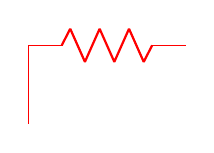
\begin{tikzpicture}
    \draw[color=red] (0,0) to[R] +(2,0) +(0,0) -- ++(0,-1);
\end{tikzpicture}
\qquad
\begin{tikzpicture}
    \draw[color=blue] (0,0) to[out=30, in=120] +(2,0) +(0,0) -- ++(0,-1);
\end{tikzpicture}
\qquad
\begin{tikzpicture}
    \draw[color=purple] (0,0) to[] +(2,0) +(0,0) -- ++(0,-1);
\end{tikzpicture}
\qquad
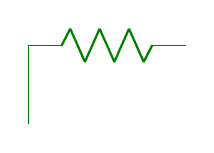
\begin{tikzpicture}
    \draw[color=green!50!black] (0,0)
        {[current point is local] to[R] +(2,0)} +(0,0) -- ++(0,-1);
\end{tikzpicture}
\end{LTXexample}


\subsubsection{Customization}
\label{sec:components-size}


Pretty much all Circui\TikZ\ relies heavily on \texttt{pgfkeys} for value handling and configuration. Indeed, at the beginning of \texttt{circuitikz.sty} and in the file \texttt{pfgcirc.define.tex}  a series of key definitions can be found that modify all the graphical characteristics of the package.

All can be varied using the \verb!\ctikzset! command, anywhere in the code.

Note that the details of the parameters that are not described in the manual can change in the future, so be ready to use a fixed version of the package (the ones with the specific number, like \verb|circuitikz-0.9.3|) if you dig into them.

\paragraph{Components size}\label{sec:pgfcircRlen}
Perhaps the most important parameter is \texttt{bipoles/length}  (default \SI{1.4}{cm}), which
can be interpreted as the length of a resistor (including reasonable connections): all other lengths are relative to this value. For instance:

\begin{LTXexample}[pos=t,varwidth=true]
\ctikzset{bipoles/length=1.4cm}
\begin{circuitikz}[scale=1.2]\draw
  (0,0) node[anchor=east] {B}
        to[short, o-*] (1,0)
        to[R=20<\ohm>, *-*] (1,2)
        to[R=10<\ohm>, v=$v_x$] (3,2) -- (4,2)
        to[cI=$\frac{\si{\siemens}}{5} v_x$, *-*] (4,0) -- (3,0)
        to[R=5<\ohm>, *-*] (3,2)
  (3,0) -- (1,0)
  (1,2) to[short, -o] (0,2) node[anchor=east]{A}
;\end{circuitikz}
\end{LTXexample}

\begin{LTXexample}[pos=t,varwidth=true]
\ctikzset{bipoles/length=.8cm}
\begin{circuitikz}[scale=1.2]\draw
  (0,0) node[anchor=east] {B}
        to[short, o-*] (1,0)
        to[R=20<\ohm>, *-*] (1,2)
        to[R=10<\ohm>, v=$v_x$] (3,2) -- (4,2)
        to[cI=$\frac{\si{\siemens}}{5} v_x$, *-*] (4,0) -- (3,0)
        to[R=5<\ohm>, *-*] (3,2)
  (3,0) -- (1,0)
  (1,2) to[short, -o] (0,2) node[anchor=east]{A}
;\end{circuitikz}
\end{LTXexample}

The changes on \texttt{bipoles/length} should, however, be globally applied to every path, because they affect every element --- including the poles. So you can have artifacts like the one in the second line below:

\begin{LTXexample}[varwidth=true]
\begin{circuitikz}[
    bigR/.style={R, bipoles/length=3cm}
    ]
    \draw (0,3) to [bigR, o-o] ++(4,0);
    \draw (0,1.5) to [bigR, o-o] ++(4,0)
      to[R, o-o] ++(2,0); % will fail here
    \draw (0,0) to [R, o-o] ++(4,0);
\end{circuitikz}
\end{LTXexample}

Several groups of components, on the other hand, have a special \texttt{scale} parameter that can be used safely in this case (starting with 0.9.4 --- more groups of components will be added going forward); the key to use will be explained in the specific description of the components. For example, in the case of resistors you have \texttt{resistors/scale} available:

\begin{LTXexample}[varwidth=true]
\begin{circuitikz}[
    bigR/.style={R, resistors/scale=1.8}
    ]
    \draw (0,3) to [bigR, o-o] ++(4,0);
    \draw (0,1.5) to [bigR, o-o] ++(4,0)
      to[R, o-o] ++(2,0); % ok now
    \draw (0,0) to [R, o-o] ++(4,0);
\end{circuitikz}
\end{LTXexample}

Never use \texttt{scale}, \texttt{xscale} or~\texttt{yscale} in a path-style component (i.e., inside a \texttt{to[...]}) command.

\paragraph{Mirroring and flipping path-style components}\label{sec:mirror-flip-path}

To change the orientation of path-style components, \emph{never} use \texttt{xscale=-1} nor~\texttt{yscale=-1}. That will mess up the path completely. Use the \texttt{mirror} and \texttt{invert}  options:
\begin{LTXexample}[varwidth=true, basicstyle=\small\ttfamily]
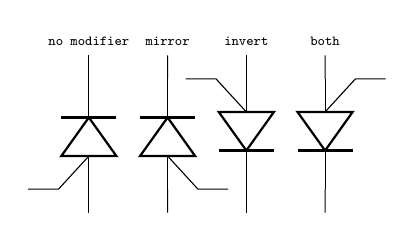
\begin{tikzpicture}[N/.style={
    font=\tiny\ttfamily, above}]
    \draw (0,0) to [put] ++(0,2)
        node[N]{no modifier};
    \draw (1,0) to [put, mirror] ++(0,2)
        node[N]{mirror};
    \draw (2,0) to [put, invert] ++(0,2)
        node[N]{invert};
    \draw (3,0) to [put, mirror, invert] ++(0,2)
        node[N]{both};
\end{tikzpicture}
\end{LTXexample}

\paragraph{Thickness of the lines}\label{sec:legacy-thickness} (globally)

The best way to alter the thickness of components is using styling, see section~\ref{sec:styling-thickness}. Alternatively, you can use ``legacy'' classes like \texttt{bipole}, \texttt{tripoles} and so on ---
for example changing the parameter \texttt{bipoles/thickness} (default 2). The number is relative to the thickness of the normal lines leading to the component.

\begin{LTXexample}[varwidth=true]
    \ctikzset{bipoles/thickness=1}
    \tikz \draw (0,0) to[C=1<\farad>] (2,0); \par
    \ctikzset{bipoles/thickness=4}
    \tikz \draw (0,0) to[C=1<\farad>] (2,0);
\end{LTXexample}

\paragraph{Shape of the components} (on a per-component-class basis)

The shape of the components are adjustable with a lot of parameters; in this manual we will comment the main ones, but you can look into the source files specified above to find more.
\begin{LTXexample}[varwidth=true]
    \tikz \draw (0,0) to[R=1<\ohm>] (2,0); \par
    \ctikzset{bipoles/resistor/height=.6}
    \tikz \draw (0,0) to[R=1<\ohm>] (2,0);
\end{LTXexample}

It is recommended to use the styling parameters to change the shapes; they are not so fine-grained (for example, you can change the width of resistor, not the height at the moment), but they are more stable and coherent across your circuit.

\subsubsection{Descriptions}

The typical entry in the component list will be like this:

\begin{groupdesc}
    \circuitdescbip{resistor}{resistor, american style}{R, american resistor}
    \circuitdescbip[potentiometer]{pR}{potentiometer, american style}{pR, american potentiometer}( wiper/0/0.3 )
\end{groupdesc}

where you have all the needed information about the bipole, with also no-standard anchors. If the component can be filled it will be specified in the description. In addition, as an example, the component shown will be filled with the option \texttt{fill=cyan!30!white}:

\begin{groupdesc}
    \circuitdescbip*{ammeter}{Ammeter}{}
\end{groupdesc}

The \emph{Class} of the component (see section~\ref{sec:styling}) is printed at the end of the description.

Most path-style components can be used as a node-style components; to access them, normally you add a \texttt{shape} to the main name of component (for example, \texttt{diodeshape}). Sometimes though the ``node name'' is different, so it is specified in the description of each component.

\subsection{Node-style components}
Node-style components (monopoles, multipoles) can be drawn at a specified point with this syntax, where \verb!#1! is the name of the component:
\begin{lstlisting}
\begin{circuitikz}
    \draw (0,0) node[#1,#2] (#3) {#4};
\end{circuitikz}
\end{lstlisting}
\noindent
Explanation of the parameters:\\
\texttt{\#1}: component name\footnote{For using bipoles as nodes, the name of the node is \texttt{\#1shape}.} (mandatory)\\
\texttt{\#2}: list of comma-separated options (optional)\\
\texttt{\#3}: name of an anchor (optional)\\
\texttt{\#4}: text written to the text anchor of the component (optional)\\


\begin{framed}
	\noindent \textbf{Notice:}	Nodes must have curly brackets at the end, even when empty. An optional anchor (\texttt{\#3}) can be defined within round brackets to be addressed again later on. And please don't forget the semicolon to terminate the \texttt{\textbackslash draw} command.
\end{framed}

\begin{framed}
	\noindent\textbf{Also notice:} If using the \verb!\tikzexternalize! feature, as of \TikZ\ 2.1 all pictures must end with \verb!\end{tikzpicture}!. Thus you \emph{cannot} use the \verb!circuitikz! environment.

	\noindent Which is OK: just use the environment \verb!tikzpicture!: everything will work there just fine.
\end{framed}

\subsubsection{Mirroring and flipping}\label{sec:mirroring-and-flipping}

Mirroring and flipping of node components is obtained by using the \TikZ\ keys \texttt{xscale} and \texttt{yscale}. Notice that these parameters also affect text labels, so they need to be un-scaled by hand. Notice that you \textbf{do not} use \texttt{xscale} or~\texttt{yscale} in a path-style component, see section~\ref{sec:mirror-flip-path} for that case.

\begin{LTXexample}[varwidth=true]
\begin{circuitikz}[scale=0.7, transform shape]
    \draw (0,3) node[op amp]{OA1};
    \draw (3,3) node[op amp, xscale=-1]{OA2};
    \draw (0,0) node[op amp]{OA3};
    \draw (3,0) node[op amp, xscale=-1]{%
        \scalebox{-1}[1]{OA4}};
\end{circuitikz}
\end{LTXexample}

To simplify this task, \Circuitikz{} has three helper macros --- \verb|\ctikzflipx{}|,
\verb|\ctikzflipy{}|, and \verb|\ctikzflipxy{}|, that can be used to ``un-rotate''
the text of nodes drawn with, respectively,
\texttt{xscale=-1}, \texttt{yscale=-1}, and \texttt{scale=-1} (which is equivalent to
\texttt{xscale=-1, yscale=-1}).

\begin{LTXexample}[varwidth=true]
\begin{circuitikz}[scale=0.7, transform shape]
    \draw (0,3) node[op amp]{OA1};
    \draw (3,3) node[op amp, xscale=-1]{\ctikzflipx{OA2}};
    \draw (0,0) node[op amp, yscale=-1]{\ctikzflipy{OA3}};
    \draw (3,0) node[op amp,  scale=-1]{\ctikzflipxy{OA4}};
\end{circuitikz}
\end{LTXexample}


\subsubsection{Anchors}

Node components anchors vary a lot across the various kinds of components, so they will be described better after each category is presented in the manual. In general all components have geographic anchors (\texttt{north}, \texttt{north west}, \dots), but most of the other anchors are very component-specific.

\subsubsection{Descriptions}

The typical entry in the component list will be like this:
\begin{groupdesc}
    \circuitdesc{cute spdt down arrow}{Cute spdt down with arrow}{}
    \circuitdesc{npn}{\scshape npn}{}( B/180/0.2,C/0/0.2,E/0/0.2 )
\end{groupdesc}

If the component can be filled it will be specified in the description. In addition, as an example, the component shown will be filled with the option \texttt{fill=cyan!30!white}:

\begin{groupdesc}
    \circuitdesc*{plain amp}{Plain amplifier}{}( out/45/0.3 )
\end{groupdesc}

Sometime, components will expose internal (sub-)shapes that can be accessed with the syntax \texttt{\textsl{<node name>}-\textsl{<internal node name>}} (a dash is separating the node name and the internal node name); that will be shown in the description as a blue ``anchor'':

\begin{groupdesc}
\circuitdesc{rotaryswitch}{Rotary switch}{}(in/-180/0.2, cin/145/0.2, center/-90/0.2, mid/0/0.4, out 1/0/0.2,
cout 1/180/0.2)[out 1.n/90/0.2, out 4.w/0/0.3]
\end{groupdesc}

The \emph{Class} of the component (see section~\ref{sec:styling}) is printed at the end of the description.

\subsection{Styling circuits and components}\label{sec:relative-size}\label{sec:styling}

You can change the visual appearance of a circuit by using a circuit style different from the default. For styling the circuit, the concept of \emph{class} of a component is key: almost every component has a class, and a style change will affect all the components of that class.

\begingroup % protect from style change the rest of the manual

Let's see the effect over a simple circuit\footnote{This is a just an example, the circuit is not intended to be functional.}.

\begin{lstlisting}[basicstyle=\scriptsize\ttfamily]
\begin{circuitikz}[american, cute inductors]
    \node [op amp](A1){\texttt{OA1}};
    \draw (A1.-) to[short] ++(0,1) coordinate(tmp) to[R, l_=$R$] (tmp -| A1.out) to[short] (A1.out);
    \draw (tmp) to[short] ++(0,1) coordinate(tmp) to[C=$C$] (tmp -| A1.out) to[short] (A1.out);
    \draw (A1.+) to [battery2, invert] ++(0,-2.5) node[ground](GND){};
    \draw (A1.-) to [L=$L$] ++(-2,0) coordinate(tmp) to[sV, l=$v_s$, fill=yellow] (tmp |-GND) node[ground]{};
    \draw (A1.out) to[R=$R_s$] ++(2,0) coordinate(bb) to[I, l_=$I_B$, invert] ++(0,2) node[vcc](VCC){};
    \draw (bb) to[D, l=$D$, *-] ++(0,-2) coordinate(bb1) to[R=$R_m$] ++(0,-2) node[vee](VEE){};
    \draw (bb) --++(1,0) node[npn, anchor=B](Q1){Q1};
    \draw (bb1) --++(1,0) node[pnp, anchor=B](Q2){Q2};
    \draw (Q1.E) -- (Q2.E) ($(Q1.E)!0.5!(Q2.E)$) to [short, *-o, name=S]  ++(2.5,0)
    node[right]{$v_{o_Q}$};
    \draw (S.s) to[european resistor, l=$Z_L$, *-] (S.s|-GND) node[ground]{};
    \draw (Q1.C) -- (Q1.C|-VCC) node[vcc]{\SI{5}{V}};
    \draw (Q2.C) -- (Q2.C|-VEE) node[vee]{\SI{-5}{V}};
\end{circuitikz}
\end{lstlisting}

This code, with the default parameters, will render like the following image.

\long\def\tmpcirc#1#2{% Define the circuit to reuse it
% \begin{center}
\begin{circuitikz}[american, cute inductors, #1]
    #2
    \node [op amp](A1){\texttt{OA1}};
    \draw (A1.-) to[short] ++(0,1) coordinate(tmp) to[R, l_=$R$] (tmp -| A1.out) to[short] (A1.out);
    \draw (tmp) to[short] ++(0,1) coordinate(tmp) to[C=$C$] (tmp -| A1.out) to[short] (A1.out);
    \draw (A1.+) to [battery2, invert, l=$v_{io}$] ++(0,-2.5) node[ground](GND){};
    \draw (A1.-) to [L=$L$] ++(-2,0) coordinate(tmp) to[sV, l=$v_s$, fill=yellow] (tmp |-GND) node[ground]{};
    \draw (A1.out) to[R=$R_s$] ++(2,0) coordinate(bb) to[I, l_=$I_B$, invert] ++(0,2) node[vcc](VCC){};
    \draw (bb) to[D, l=$D$, *-] ++(0,-2) coordinate(bb1) to[R=$R_m$] ++(0,-2) node[vee](VEE){};
    \draw (bb) --++(1,0) node[npn, anchor=B](Q1){Q1};
    \draw (bb1) --++(1,0) node[pnp, anchor=B](Q2){Q2};
    \draw (Q1.E) -- (Q2.E) ($(Q1.E)!0.5!(Q2.E)$) to [short, *-o, name=S]  ++(2.5,0)
    node[right]{$v_{o_Q}$};
    \draw (S.s) to[european resistor, l=$Z_L$, *-] (S.s|-GND) node[ground]{};
    \draw (Q1.C) -- (Q1.C|-VCC) node[vcc]{\SI{5}{V}};
    \draw (Q2.C) -- (Q2.C|-VEE) node[vee]{\SI{-5}{V}};
\end{circuitikz}%
% \end{center}
}

\tmpcirc{}{}

\subsubsection{Relative size}\label{sec:styling-scale}

Component size can be changed globally (see section~\ref{sec:pgfcircRlen}), or you can change their relative size by scaling a family of components by setting the key \texttt{\emph{class}/scale}; for example, you can change the size of all the diodes in your circuit by setting \texttt{diodes/scale} to something different from the default \texttt{1.0}.

Remember that if you use a global scale (be sure to read section~\ref{sec:bugs}!) you change the coordinate only, so using \texttt{scale=0.8} in the environment options you have:

\tmpcirc{scale=0.8}{}

If you want to scale all the circuit, you have to use also \texttt{transform shape}:

\tmpcirc{scale=0.8, transform shape}{}

Using relative sizes as described in section~\ref{sec:pgfcircRlen} enables your style for the circuit. For example,  setting:

\begin{lstlisting}
    \ctikzset{resistors/scale=0.8,      % smaller R
        capacitors/scale=0.7,           % even smaller C
        diodes/scale=0.6,               % small diodes
        transistors/scale=1.3}          % bigger BJTs
\end{lstlisting}

Will result in a (much more readable in Romano's opinion) circuit:

\tmpcirc{scale=0.8, transform shape}{\ctikzset{resistors/scale=0.8, capacitors/scale=0.7, diodes/scale=0.6, transistors/scale=1.3}}

\textbf{Warning:} relative scaling is meant to work for a reasonable range of stretching and shortening, so try to  keep your scale parameter in the \texttt{0.5} to~\texttt{2.0} range (more or less). Bigger or smaller value can result in awkward shapes.

\subsubsection{Fill color}\label{sec:styling-fillcolor}

You can also set a default fill color for the  components. You can use the keys \texttt{\emph{class}/fill} (which defaults to \texttt{none}, no fill, i.e. transparent component) for all fillable components in the library.

If you add to the previous styles the following commands:

\begin{lstlisting}
\ctikzset{
    amplifiers/fill=cyan,
    sources/fill=green,
    diodes/fill=red,
    resistors/fill=violet,
}
\end{lstlisting}

you will have the following circuit (note that the first generator is \emph{explicitly} set to be yellow,
so if will not be colored green!):

\tmpcirc{scale=0.8, transform shape}{\ctikzset{resistors/scale=0.8, capacitors/scale=0.7, diodes/scale=0.6, transistors/scale=1.3,%
             amplifiers/fill=cyan, sources/fill=green, diodes/fill=red, resistors/fill=violet,}}

Please use this option with caution. Although two-colors circuits can be nice, using more than that can become rapidly unbearable.
Old textbooks used the two-color style quite extensively, filling with a kind of light blue like \texttt{blue!30!white} ``closed'' components, but that was largely to hinder black-and-white photocopying\dots

\subsubsection{Line thickness}\label{sec:styling-thickness}

You can change the line thickness for any class of component in an independent way. The default standard thickness of components is defined on a loose ``legacy'' category (like \texttt{bipoles}, \texttt{tripoles} and so on, see section~\ref{sec:legacy-thickness}); to override that you set the key \texttt{\emph{class}/thickness} to any number. The default is \texttt{none}, which means that the old way of selecting thickness is used.

For example, \emph{amplifiers} have the legacy class of \texttt{tripoles}, as well as transistors and tubes. By default they are drawn with thickness 2 (relative to the base linewidth). To change them to be thicker, you can for example add to the previous style

\begin{lstlisting}
    \ctikzset{amplifier/thickness=4}
\end{lstlisting}

\tmpcirc{scale=0.8, transform shape}{\ctikzset{resistors/scale=0.8, capacitors/scale=0.7, diodes/scale=0.6, transistors/scale=1.3,%
             amplifiers/fill=cyan, sources/fill=green, diodes/fill=red, resistors/fill=violet,
            amplifiers/thickness=4}}

\textbf{Caveat:} not every component has a ``class'', so you have to play with the available ones (it's specified in the component description) and with the absolute values to have the circuit following your taste. A bit of experimentation will create a kind of \emph{style options} that you could use in all your documents.

\subsubsection{Style files}

When using styles, it is possible to use \emph{style files} (see section~\ref{sec:writingstylefiles}), that then you can load with the command \verb|\ctikzloadstyle|. For example, in the distribution you have a number of style files: \texttt{legacy}, \texttt{romano}, \texttt{example}. When you load a style name \texttt{\emph{name}}, you will have available a style called \texttt{\emph{name} circuit style} that you can apply to your circuits.
The last style loaded is not enacted --- you have to explicitly do it if you want the style used by default, by putting for example in the preamble:

\begin{lstlisting}[numbers=none]
    \ctikzloadstyle{romano}
    \tikzset{romano circuit style}
\end{lstlisting}

Please notice that the style is at \TikZ{} level, not \Circuitikz --- that let's you use it in the top option of the circuit, like:

\begin{lstlisting}[numbers=none]
    \begin{circuitikz}[legacy circuit style,
    ..., ]
    ...
    \end{circuitikz}
\end{lstlisting}

If you just want to use one style, you can load and activate it in one command with

\begin{lstlisting}[numbers=none]
    \ctikzsetstyle{romano}
\end{lstlisting}

The \texttt{example} style file will simply make the amplifiers filled with light blue:

\begin{LTXexample}[varwidth=true]
\begin{circuitikz}
    \draw (0,0) node[op amp]{OA1};
\end{circuitikz}
\ctikzloadstyle{example}
\begin{circuitikz}[example circuit style]
    \draw (0,0) node[op amp]{OA1};
\end{circuitikz}
\end{LTXexample}
\ctikzloadstyle{legacy}
\ctikzloadstyle{romano}

The style \texttt{legacy} is a style that set (most) of the style parameters to the default, and \texttt{romano} is a style used by one of the authors; you can use these styles as is or you can use them to learn to how to write new file style following the instructions in section~\ref{sec:writingstylefiles}. In the next diagrams, the left hand one is using the \texttt{romano circuit style} and the rigth hand one the legacy style.

\fbox{\tmpcirc{scale=0.6, transform shape, romano circuit style}{}}
\fbox{\tmpcirc{scale=0.6, transform shape, legacy circuit style}{}}

\endgroup % restore state before example of sizing

\subsubsection{Style files: how to write them}\label{sec:writingstylefiles}

The best option is to start from \texttt{ctikzstyle-legacy.tex} and edit your style file from it. Then you just put it in your input path and that's all. If you want, you can contribute your style file to the project.

Basically, to write the style \texttt{example}, you edit a file named \texttt{ctikzstyle-romano.tex} with will define and enact \TikZ\ style with name \texttt{example circuit style}; basically it has to be something along this:

\lstinputlisting[frame=single, framesep=10pt]{ctikzstyle-example.tex}

This kind of style will \emph{add} to the existing style.  If you want to have a style that \emph{substitutes} the current style, you should do like this:

\begin{lstlisting}[frame=single, framesep=10pt]
\ctikzloadstyle{legacy}% start from a known state
\tikzset{romano circuit style/.style={%
    legacy circuit style, % load the legacy style
    \circuitikzbasekey/.cd,%
    % Resistors
    resistors/scale=0.8,
[...]
    }}
\end{lstlisting}

If you want to add a setting to your style file that has been recently added to the package (for example, the thyristor compact shapes added in \texttt{1.3.5}), but you want your style file to be still compatible with older versions of \Circuitikz, you can use the \texttt{.try} statement:

\begin{lstlisting}[frame=single, framesep=10pt]
    % Diodes
    diodes/scale=0.6,
    diodes/thickness=1.0,
    thyristor style/.try=compact,
\end{lstlisting}

Or, in case of new values of existing ``choice'' keys, you can use the syntax:

\begin{lstlisting}[frame=single, framesep=10pt]
    % Logic ports
    logic ports/ieee/.try,
    % this way of setting the key does nothing if ieee option
    % does not exist; logic ports/.try=ieee does not work
    % if the key exists but the value is not defined
    logic ports/scale=1.0,
\end{lstlisting}


\subsection{Subcircuits}\label{sec:subcircuits}

Starting from version \texttt{1.3.5}, there is support for generating sub-circuits, or circuit blocks. The creation and use of subcircuits is somewhat limited, to keep them simple and easy to define and maintain.

A subcircuit is basically a path (and just one path!) of generic \TikZ{} instructions, with a series of accessible coordinates that behave more or less like anchors in the ``real'' shapes. The basic limitation is that a subcircuit can be moved, replicated and placed around but it can't be easily personalized. Even if scaling and rotation is in principle possible, it is not easily done. Nevertheless, they can be quite useful to build complex components and reusable blocks.

\subsubsection{Subcircuit definition}

To define a block you use the \verb|\ctikzsubcircuitdef| macro; this macro has 3 arguments:
\begin{itemize}
    \item the first argument is the name of the subcircuit, and it must form a valid TeX command name when prepended with a backslash: so just letters (no spaces, nor numbers, nor symbols like underscores, etc.);
    \item the second one is a comma-separated list of anchor names; here you can use whatever you can use for naming a coordinate or a node (so it's much more relaxed than the first one);
\item finally, the commands that will draw the circuit. You must suppose you are in a \verb|\draw| command, with the start coordinate already set-up. You can (and should) use \verb|#1| as the name of the current node, and you \emph{must} define the coordinates of all the anchors listed before as \texttt{coordinate(\#1-\emph{anchorname})}. You should \textbf{not} finish the path here and use \textbf{only relative coordinates} or \textbf{named ones}.
\end{itemize}

Let's see that with an example:

\ctikzsubcircuitdef{optovishay}{in 1, out 1, in 2, out 2, center}{%
    % reference anchor is -center
    coordinate(#1-center)
    (#1-center) +(-1.2,-1) rectangle +(1.2,1)
    (#1-center) ++(-1.2,0.8) coordinate (#1-in 1)
    (#1-center) ++(-1.2,-0.8) coordinate (#1-in 2)
    (#1-center) ++(1.2,0.8) coordinate (#1-out 1)
    (#1-center) ++(1.2,-0.8) coordinate (#1-out 2)
    (#1-center) ++(0,1) coordinate (#1-up)
    (#1-in 1) -- ++(0.5,0) coordinate(#1-tmp)
        to[leD*, diodes/scale=0.6, led arrows from cathode]
        (#1-tmp|- #1-in 2) -- (#1-in 2)
    (#1-out 1) -- ++(-0.5,0) coordinate(#1-tmp)
        to[pD*, diodes/scale=0.4, mirror]  ++(0,-0.5)
        edge[densely dashed] ++(0,-0.533) ++(0,-0.566)
        to[pD*, diodes/scale=0.4,mirror] (#1-tmp|- #1-out 2) -- (#1-out 2)
    % leave the position of the path at the center
    (#1-center)
}
\begin{lstlisting}
\ctikzsubcircuitdef{optovishay}{in 1, out 1, in 2, out 2, center}{%
    % reference anchor is -center
    coordinate(#1-center)
    (#1-center) +(-1.2,-1) rectangle +(1.2,1)
    (#1-center) ++(-1.2,0.8) coordinate (#1-in 1)
    (#1-center) ++(-1.2,-0.8) coordinate (#1-in 2)
    (#1-center) ++(1.2,0.8) coordinate (#1-out 1)
    (#1-center) ++(1.2,-0.8) coordinate (#1-out 2)
    (#1-center) ++(0,1) coordinate (#1-up)
    (#1-in 1) -- ++(0.5,0) coordinate(#1-tmp)
        to[leD*, diodes/scale=0.6, led arrows from cathode]
        (#1-tmp|- #1-in 2) -- (#1-in 2)
    (#1-out 1) -- ++(-0.5,0) coordinate(#1-tmp)
        to[pD*, diodes/scale=0.4, mirror]  ++(0,-0.5)
        edge[densely dashed] ++(0,-0.533) ++(0,-0.566)
        to[pD*, diodes/scale=0.4,mirror] (#1-tmp|- #1-out 2) -- (#1-out 2)
    % leave the position of the path at the center
    (#1-center)
}
\end{lstlisting}

Our element is a symbol for an optocoupler; in this case is the symbol used for one cell of the double \href{https://www.vishay.com/docs/84639/vo1263aa.pdf}{Vishay vo1263 device}.

The name of the subcircuit is \texttt{optovishay} --- notice we can use only letters here, upper or lowercase, and nothing more.
Then we have a series of anchor names; here we can use letters, numbers, spaces and some symbol --- but avoid the dot (\texttt{.}) and the hyphen (\texttt{-}).
Additionally, the anchor named \texttt{subckt@reference} is reserved and shouldn't be used.
If you use spaces, be on the safe side and \emph{never} use two or more consecutive spaces.

After that, you have to draw your subcircuit as if you were into a \verb|\draw| command, starting from a generic point.
In this case, we decide to draw the circuit around this generic point so that it will result to be the center of the block; so as a first thing, we ``mark'' the position of the center anchor, with \texttt{coordinate(\#1-center)}.
The \texttt{\#1} will be substituted with the specific name of the subcircuit's instance later --- so if you then call one instance of the optocoupler \texttt{opto1}, that coordinate will be called \texttt{opto1-center}.

We continue by defining all our anchors (there is no need to do that at the start, but it's handy because then you can use them).
You \textbf{must} define all the anchors!

\textbf{Important}: all the coordinates used must be either relative, or named in the form \texttt{\#1-something}; absolute coordinate will not work when instantiating the block.
The block is thought to be used inside a path specification, so the idea is not to end the path --- that means that changing line styles or colors is at best difficult.
You can still use \texttt{edge}s, though (see~\ref{faqs:dashed}).

After that, we draw our circuit; in this case a LED and a couple of smaller photodiodes will do.
We also define a coordinate \texttt{-up} (you can define more coordinates, in addition to the anchors, or name elements with \texttt{name=\#1-\emph{something}} for later access) for adding text.

\subsubsection{Using the subcircuit}

To use the subcircuit, an additional step is needed. Somewhere you have to \emph{activate} it. This is needed to calculate the relative positions of anchors using the current set of style parameters. The normal place is to activate it just before usage; to do that you use the command \verb|\ctikzsubcircuitactivate| with the name of the subcircuit. That will define a new command, \texttt{\textbackslash\emph{nameofthesubcircuit}} that you can use then in your paths.

So to check your subcircuit while defining it you can use this simple snippet:
\begin{LTXexample}[varwidth=true]
\ctikzsubcircuitactivate{optovishay}
\begin{tikzpicture}
    \draw (0,0) \optovishay{one}{};
    \node [above] at (one-up) {O1};
    \draw[color=blue] (one-out 1) -- ++(1,0)
        \optovishay{two}{in 1};
    \node [above] at (two-up) {O2};
\end{tikzpicture}
\end{LTXexample}

\paragraph{Scaling, flipping and rotating subcircuits}

To scale and rotate a subcircuit you have to include it into a \texttt{scope} with the appropriate \texttt{scale} and rotation commands. Notice that, as in general in \Circuitikz, global scales that affect rotation works only if \texttt{transform shape} is issued (see~\ref{sec:bugs}); nesting \texttt{transform shape} normally works, but it has been really lightly tested.

\begin{LTXexample}[varwidth=true]
\ctikzsubcircuitactivate{optovishay}
\begin{tikzpicture}[scale=0.8, transform shape]
    \draw (0,0) \optovishay{three}{};
    \draw (three-out 1) -- ++(0.5,0) coordinate(here);
    \begin{scope}[xscale=-1,rotate=-45,transform shape]
        \draw (here) \optovishay{four}{out 1};
    \end{scope}
    \draw[blue] (three-out 2) -| (four-out 2);
\end{tikzpicture}
\end{LTXexample}

\subsubsection{Parameters in subcircuits}

There are no additional parameters definable for subcircuit shapes; this is a bit of a pity, because sometimes they could be useful, especially for labels of objects.
Given the need to use \texttt{transform shape} to translate and rotate them, though, it is better not to add invariant-direction things (like text) into the subcircuit, unless you are sure you will just translate them.
One possibility is to use additional macros and anchors for positioning, like in the following example.

Suppose you have defined

\begin{lstlisting}
    \ctikzsubcircuitdef{divider}{in, out}{%
        coordinate (#1-in) to[R, l=~, name=#1-rh, -*] ++(2,0)
        coordinate(#1-tmp) to[R, l=~, name=#1-rl] ++(0,-2)
        node[tlground]{} (#1-tmp) --++(0.5,0) coordinate(#1-out)
    }
\end{lstlisting}

\ctikzsubcircuitdef{divider}{in, out}{%
    coordinate (#1-in) to[R, l=~, name=#1-rh, -*] ++(2,0)
    coordinate(#1-tmp) to[R, l=~, name=#1-rl] ++(0,-2)
    node[tlground]{} (#1-tmp) --++(0.5,0) coordinate(#1-out)
}

then you can additionally define:

\begin{lstlisting}
    \newcommand{\mydiv}[4]{
        \divider{#1}{#2} (#1-rh.n) node[above]{#3}
        (#1-rl.n) node[right]{#4} (#1-out)
    }
\end{lstlisting}

\newcommand{\mydiv}[4]{
    \divider{#1}{#2} (#1-rh.n) node[above]{#3}
    (#1-rl.n) node[right]{#4} (#1-out)
}

And finally do:
\begin{LTXexample}[varwidth=true]
\ctikzsubcircuitactivate{divider}
\begin{tikzpicture}
    \draw (0,0) \mydiv{a}{in}{$R_1$}{$R_2$};
    \draw (a-out) -- \mydiv{b}{in}{$R_3$}{$R_4$};
\end{tikzpicture}
\end{LTXexample}


\section{The components: list}

This section is dedicated to the full list of available components.

\subsection{Grounds and supply voltages}

Ground symbols and power supplies --- they have two different classes for styling.

\subsubsection{Grounds}

For the grounds, the \texttt{center} anchor is put on the connecting point of the symbol, so that you can use them directly in a \texttt{path} specification.

\begin{groupdesc}
    \circuitdesc{ground}{Ground}{}( center/0/0.3 )
    \circuitdesc{tlground}{Tailless ground}{}( center/0/0.3 )
    \circuitdesc{rground}{Reference ground}{}
    \circuitdesc*{sground}{Signal ground}{}
    \circuitdesc{tground}{Thicker tailless reference ground}{}
    \circuitdesc{nground}{Noiseless ground}{}
    \circuitdesc*{pground}{Protective ground}{}
    \circuitdesc{cground}{Chassis ground\footnotemark}{}
    \footnotetext{These last three were contributed by Luigi «Liverpool»}
    \circuitdesc{eground}{European style ground}{}
    \circuitdesc{eground2}{European style ground, version 2\footnotemark}{}
    \footnotetext{These last two were contributed by \texttt{@fotesan}}
\end{groupdesc}

\paragraph{Grounds anchors}

Anchors for grounds are a bit strange, given that they have the \texttt{center} spot at the same location than \texttt{north} and all the ground will develop ``going down'':

\showanchors[baseline]{ground, scale=1.5}{}(north/90/0.4, north east/45/0.4, east/0/0.4, south east/-45/0.4,
    south/-90/0.4, south west/-135/0.4, west/180/0.4, north west/135/0.4)
\showanchors[baseline]{ground, scale=1.5}{}(left/135/0.2, right/45/0.2, center/-180/0.2)

\paragraph{Grounds customization}

You can change the scale of these components (all the ground symbols together) by setting the key \texttt{grounds/scale} (default \texttt{1.0}).

\subsubsection{Power supplies}

\begin{groupdesc}
    \circuitdesc{vcc}{VCC/VDD}{}
    \circuitdesc{vee}{VEE/VSS}{}
\end{groupdesc}

The power supplies are normally drawn with the arrows shown in the list above.

\paragraph{Power supply anchors}

They are similar to ground anchors, and the geographical anchors are correct only for the default arrow.

\showanchors[baseline]{vcc, scale=1.5}{}(north/90/0.4, north east/45/0.4, east/0/0.4, south east/-45/0.4,
    south/-90/0.4, south west/-135/0.4, west/180/0.4, north west/135/0.4)
\showanchors[baseline]{vcc, scale=1.5}{}(left/135/0.2, right/45/0.2, center/-180/0.2)


\paragraph{Power supplies customization}

You can change the scale of the power supplies by setting the key \texttt{power supplies/scale} (default \texttt{1.0}).

Given that the power supply symbols are basically arrows, you can change them using all the options of the \texttt{arrows.meta} package (see the \TikZ\ manual for details) by changing the keys \texttt{monopoles/vcc/arrow} and \texttt{monopoles/vee/arrow} (the default for both is \texttt{legacy}, which will use the old code for drawing them).
Note that the anchors are at the start of the connecting lines, and that geographical anchors are just approximation if you change the arrow symbol!

\begin{LTXexample}[varwidth=true]
\begin{circuitikz}
    % next macro is available in ctikzmanutils.sty
    \def\coord(#1){\showcoord(#1)<0:0.3>}
    \draw (0,0)
    node[vcc](vcc){VCC} \coord(vcc) ++(2,0)
    node[vee](vee){VEE} \coord(vee);
    \ctikzset{monopoles/vcc/arrow={Stealth[red, width=6pt, length=9pt]}}
    \ctikzset{monopoles/vee/arrow={Latex[blue]}}
    \draw (0,-2)
    node[vcc](vcc){VCC} \coord(vcc) ++(2,0)
    node[vee](vee){VEE} \coord(vee);
\end{circuitikz}
\end{LTXexample}

However, arrows in \TikZ{} are in the same class with the line thickness, so they do not scale with neither the class \texttt{power supplies} scale nor the global scale parameter (you should use \texttt{transform canvas=\{scale\dots\}} for this).

If you want the arrows to behave like the legacy symbols (which are shapes), \emph{only in the arrow definitions}, you can use the special length parameter \verb|\scaledwidth|\footnote{Thanks to @Schrödinger's cat on \href{https://tex.stackexchange.com/a/506249/38080}{\TeX{} stackexchange site}} in the arrow definition, which correspond to the width of the legacy \texttt{vcc} or \texttt{vee}. Compare the effects on the following circuit.

\begin{LTXexample}[pos=t]
\ctikzset{%
    monopoles/vcc/arrow={Triangle[width=0.8*\scaledwidth, length=\scaledwidth]},
    monopoles/vee/arrow={Triangle[width=6pt, length=8pt]},
}
\begin{circuitikz}[baseline=(vo.center)]
    \node [ocirc](TW) at (0,0) {};
    \draw (TW.east) -- ++(1,0) node[midway, above]{$v_i$} node[op amp, anchor=-](A1){};
    \draw (A1.up)   -- ++(0, 0.3) node[vcc]{\SI{+10}{V}};
    \draw (A1.down) -- ++(0,-0.3) node[vee]{\SI{-10}{V}};
    \draw (A1.+) -- ++(-0.5,0) to[battery2, invert, l_=\SI{2}{V}] ++(0,-1) node[ground]{};
    \draw (A1.out) to[short, -o] ++(0.5,0) node[above](vo){$v_o$};
\end{circuitikz} \qquad
\begin{circuitikz}[baseline=(vo.center), scale=0.6, transform shape]
    \node [ocirc](TW) at (0,0) {};
    \draw (TW.east) -- ++(1,0) node[midway, above]{$v_i$} node[op amp, anchor=-](A1){};
    \draw (A1.up)   -- ++(0, 0.3) node[vcc]{\SI{+10}{V}};
    \draw (A1.down) -- ++(0,-0.3) node[vee]{\SI{-10}{V}};
    \draw (A1.+) -- ++(-0.5,0) to[battery2, invert, l_=\SI{2}{V}] ++(0,-1) node[ground]{};
    \draw (A1.out) to[short, -o] ++(0.5,0) node[above](vo){$v_o$};
\end{circuitikz}
\end{LTXexample}


\subsection{Resistive bipoles}

\begin{groupdesc}
    \circuitdescbip{short}{Short circuit}{}
    \circuitdescbip{open}{Open circuit}{}
    \circuitdescbip*{generic}{Generic (symmetric) bipole}{}
    \circuitdescbip*{xgeneric}{Crossed generic (symmetric) bipole}{}
    \circuitdescbip*{tgeneric}{Tunable generic bipole}{}
    \circuitdescbip*{ageneric}{Generic asymmetric bipole}{}
    \circuitdescbip*{memristor}{Memristor}{Mr}
\end{groupdesc}

Both \texttt{shortshape} and \texttt{openshape} are not really supposed to be used; they are dummy shapes used as placeholders for the path-drawing routines.

If \texttt{americanresistors} option is active (or the style \texttt{[american resistors]} is used --- this is the default for the package), the resistors are displayed as follows:
\begin{groupdesc}
    \ctikzset{resistor=american}
    \circuitdescbip[resistor]{R}{Resistor}{american resistor}
    \circuitdescbip[vresistor]{vR}{Variable resistor}{variable american resistor}(wiper/180/0.3, tip/0/0.3)
    \circuitdescbip[potentiometer]{pR}{Potentiometer}{american potentiometer}(wiper/0/0.3, tip/135/0.2)
    \circuitdescbip[resistivesens]{sR}{Resistive sensor}{american resistive sensor}(label/0/0.3, wiper/180/0.3, tip/0/0.3)
    \circuitdescbip*[ldresistor]{ldR}{Ligth-Dependent resistor}{american light dependent resistor}(arrows/-45/0.3)
\end{groupdesc}

If  instead \texttt{europeanresistors} option is active (or the style \texttt{[european resistors]} is used), the resistors, variable resistors and potentiometers are displayed as follows:
\begin{groupdesc}
    \ctikzset{resistor=european}
    \circuitdescbip*[generic]{R}{Resistor}{european resistor}
    \circuitdescbip*[tgeneric]{vR}{Variable resistor}{variable european resistor}(wiper/180/0.3, tip/0/0.3)
    \circuitdescbip*[genericpotentiometer]{pR}{Potentiometer}{european potentiometer}(wiper/0/0.3, tip/135/0.2)
    \circuitdescbip*[thermistor]{sR}{Resistive sensor}{european resistive sensor}(label/0/0.3, wiper/180/0.3, tip/0/0.3)
    \circuitdescbip*[ldgeneric]{ldR}{Ligth-Dependent resistor}{european light dependent resistor}(arrows/-45/0.3)
    \ctikzset{resistor=american} % reset default
\end{groupdesc}

Other miscellaneous resistor-like devices:
\begin{groupdesc}
    \circuitdescbip*{varistor}{Varistor}{}
    \circuitdescbip*[photoresistor]{phR}{Photoresistor}{photoresistor}(arrows/0/0.3)
    \circuitdescbip*[thermistor]{thR}{Thermistor}{thermistor}
    \circuitdescbip*[thermistorptc]{thRp}{PTC thermistor}{thermistor ptc}
    \circuitdescbip*[thermistorntc]{thRn}{NTC thermistor}{thermistor ntc}
\end{groupdesc}


\subsubsection{Potentiometers: wiper position}

Since version \texttt{0.9.5}, you can control the position of the wiper in potentiometers using the key \texttt{wiper pos}, which is a number in the range $[0,1]$. The default middle position is \texttt{wiper pos=0.5}.


\begin{LTXexample}[varwidth]
\begin{circuitikz}[american]
    \ctikzset{resistors/width=1.5, resistors/zigs=9}
    \draw (0,0) to[pR, name=A] ++(0,-4);
    \draw (1.5,0) to[pR, wiper pos=0.3, name=B] ++(0,-4);
    \ctikzset{european resistors}
    \draw (3,0) to[pR, wiper pos=0.8, name=C] ++(0,-4);
    \foreach \i in {A, B, C}
        \node[right] at (\i.wiper) {\i};
\end{circuitikz}
\end{LTXexample}

Since version \texttt{1.6.0}, potentiometers and variable resistors have extra anchors\footnote{Thanks to a suggestion by \href{https://github.com/circuitikz/circuitikz/issues/663}{Dr. Matthias Jung on GitHub}}, to allow this kind of circuit (that seems to be common in some region):

\begin{LTXexample}[varwidth=true, basicstyle=\small\ttfamily]
\begin{circuitikz}[european]
    \draw (0,0) to[battery2, l=E] ++(0,4.5)
        -- ++(2,0) coordinate(tmp)
        to[vR, l2_=$P_1$ and \SI{10}{\kohm}, mirror,
            invert, name=P]
        (0,0-|tmp) -- (0,0);
    \draw (0,0-|tmp) -- ++(1.5,0)
        to[R=$R_1$, -*] ++(0,2) coordinate(p)
        |- (P.wiper);
    \draw (p) to[rmeterwa, t=V] (tmp-|p) -- (tmp);
\end{circuitikz}
\end{LTXexample}


\subsubsection{Generic sensors anchors}\label{sec:sensors-anchors}
Generic sensors have an extra anchor named \texttt{label}  to help position the type of dependence, if needed:

\begin{LTXexample}[varwidth=true]
\begin{circuitikz}
   \draw (0,2) to[sR, l=$R$, name=mySR] ++(3,0);
   \node [font=\tiny, right] at(mySR.label) {-t\si{\degree}};
   \draw (0,0) to[sL, l=$L$, name=mySL] ++(3,0);
   \node [draw, circle, inner sep=2pt] at(mySL.label) {};
   \draw (0,-2) to[sC, l=$C$, name=mySC] ++(3,0);
   \node [font=\tiny, below right, inner sep=0pt] at(mySC.label) {+H\si{\%}};
\end{circuitikz}
\end{LTXexample}

The anchor is positioned just on the corner of the segmented line crossing the component.

\subsubsection{Resistive components customization}

\paragraph{Geometry.} You can change the scale of these components (all the resistive bipoles together) by setting the key \texttt{resistors/scale} (default \texttt{1.0}).  Similarly, you can change the widths by setting \texttt{resistors/width} (default \texttt{0.8}).

You can change the width of these components (all the resistive bipoles together) by setting the key \texttt{resistors/width}  to something different from the default \texttt{0.8}.

For the american style resistors, you can change the number of ``zig-zags'' by setting the key
\texttt{resistors/zigs} (default value \texttt{3}).

\begin{LTXexample}[varwidth=true]
\begin{circuitikz}[
        longpot/.style = {pR, resistors/scale=0.75,
        resistors/width=1.6, resistors/zigs=6}]
   \draw (0,1.5) to[R, l=$R$] ++(4,0);
   \draw (0,0) to[longpot, l=$P$] ++(4,0);
   \ctikzset{resistors/scale=1.5}
   \draw (0,-1.5) to[R, l=$R$] ++(4,0);
\end{circuitikz}
\end{LTXexample}

\paragraph{Thickness.}\label{sec:resistor-thickness} The line thickness of the resistive components is governed by the class thickness; you can change it assigning a value to the key \texttt{resistors/thickness} (default \texttt{none}, that means \texttt{bipoles/thickness} is used, and that defaults to \texttt{2.0}; the value is relative to the base line thickness).

We can call \emph{modifiers} the elements that are added to the basic shape to express some characteristics of the component; for example the arrows for the variable resistors or the bar for the sensors. Normally the thickness of these elements are the same as the one chosen for the component\footnote{Due to a bug in versions before 1.3.4, that didn't happen for thermistors}. You can change their thickness with the class key \texttt{modifier thickness} which is relative to the main component thickness.

\begin{LTXexample}[varwidth]
\begin{circuitikz}[american]
    \draw (0,2) to[vR] ++(2,0) to[sR] ++(2,0);
    \ctikzset{resistors/thickness=4}
    \draw (0,1) to[vR] ++(2,0) to[sR] ++(2,0);
    \ctikzset{resistors/modifier thickness=0.5}
    \draw (0,0) to[vR] ++(2,0) to[sR] ++(2,0);
\end{circuitikz}
\end{LTXexample}

\paragraph{Arrows.\label{sec:tunablearrows}} You can change the arrow tips used in tunable resistors (\texttt{vR}, \texttt{tgeneric}) with the key \texttt{tunable end arrow}  and in potentiometers with the key \texttt{wiper end arrow} (by default the key is the word ``\texttt{default}'' to obtain the default arrow, which is \texttt{latexslim} for both).
Also you can change the start arrow with the corresponding \texttt{tunable start arrow} or \texttt{wiper start arrow} (the default value ``\texttt{default}'' is equivalent to \texttt{\{\}} for both, which means no arrow).

You can change that globally or locally, as ever. The tip specification is the one you can find in the \TikZ{} manual (``Arrow Tip Specifications'').
For the \texttt{photoresistor} and the two ``flavors'' of the light-dependent resistor (\texttt{ldR}, american or european), the style of the arrows follow the \texttt{opto} commands as in the photodiodes and phototransistor: see~\ref{sec:opto-arrows}.

\begin{LTXexample}[varwidth]
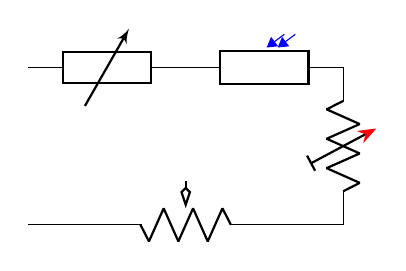
\begin{tikzpicture}[american]
    % globally all the potentiometrs
    \ctikzset{wiper end arrow={Kite[open]},
        opto arrows/color=blue, opto end arrow={Triangle}}
    \draw (0,0) to[tgeneric] ++(2,0) to[phR] ++(2,0)
    % set locally on this variable resistor
       to[vR, tunable end arrow={Stealth[red]},
       tunable start arrow={Bar}, invert] ++(0,-2)
       to[pR, mirror] ++(-4,0);
\end{tikzpicture}
\end{LTXexample}


\subsection{Capacitors and inductors: dynamical bipoles}

\subsubsection{Capacitors}

\begin{groupdesc}
    \circuitdescbip*{capacitor}{Capacitor}{C}
    \circuitdescbip*[ccapacitor]{curved capacitor}{Curved (polarized) capacitor}{cC}
    \circuitdescbip*{ecapacitor}{Electrolytic capacitor}{eC,elko}
    \circuitdescbip*[vcapacitor]{variable capacitor}{Variable capacitor}{vC}(wiper/180/0.3, tip/0/0.3)
    \circuitdescbip*[capacitivesens]{capacitive sensor}{Capacitive sensor}{sC}(label/0/0.3, wiper/180/0.3, tip/0/0.3)
    \circuitdescbip*{piezoelectric}{Piezoelectric Element}{PZ}
    \circuitdescbip*{cpe}{Constant Phase Element}{cpe}
    \circuitdescbip*[ferrocap]{feC}{Ferroelectric capacitor\footnotemark}{ferrocap}(kink left/180/0.2, kink right/0/0.2, curve left/160/0.3, curve right/-20/0.2, center/45/0.3)
    \footnotetext{suggested by \href{https://github.com/circuitikz/circuitikz/issues/515}{Mayeul Cantan}}
\end{groupdesc}

Capacitors are fillable since \texttt{v1.4.1}; this is normally just a stylistic option but in the case of
ferroelectric capacitors that could be used to show the state of the hysteresis of the component.

\begin{LTXexample}[varwidth]
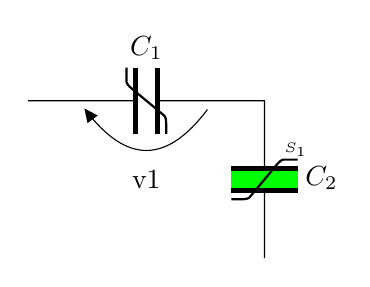
\begin{tikzpicture}[]
    \ctikzset{capacitors/.cd,
    thickness=4, modifier thickness=0.5}
    \draw (0,0) to[feC, l=$C_1$, v=v1] ++(3,0)
        to[feC, l=$C_2$, fill=green, name=C2] ++(0,-2);
    \node [font=\tiny, above right, inner sep=1pt]
        at(C2.kink left) {$S_1$};
\end{tikzpicture}
\end{LTXexample}

There is also the (deprecated\footnote{Thanks to \href{https://tex.stackexchange.com/questions/509594/polar-capacitor-orientation-in-circuitikz-seems-wrong}{Anshul Singhv for noticing}.} --- its polarity is not coherent with the rest of the components) \texttt{polar capacitor}; please do not use it.

\subsubsection{Capacitive sensors anchors}

For capacitive sensors, you have the same anchors than in the case of resistive sensors, see section~\ref{sec:sensors-anchors}.

\subsubsection{Capacitors customizations}\label{sec:capacitors-styling}

You can change the scale of the capacitors by setting the key \texttt{capacitors/scale}  to something different from the default \texttt{1.0}. For thickness, you can use the same keys (applied to the \texttt{capacitors} class) as for resistors in~\ref{sec:resistor-thickness}.

Variable capacitors arrow tips follow the settings  of resistors, see section~\ref{sec:tunablearrows}.

The relative size of the capacitors is a bit of a mixed bag, because each one has historically different internal parameters that makes maintaining coherence quite difficult. In \texttt{v1.4.1} this has changed and now you can use styling options to change the way the capacitors look. The main parameter you can set is \texttt{capacitors/width} (default \texttt{0.2}), which controls the standard distance between plates. That will change all the components (notice that \texttt{piezoelectric} and \texttt{cpe} default width is twice the size of a standard capacitor --- although this is not evident for the \texttt{cpe} given its shape.)

\begin{LTXexample}[varwidth=true, basicstyle=\small\ttfamily]
\begin{circuitikz}[european]
    \draw (0,1) to[C=aaa] ++(2,0) to[cpe=bbb] ++(2,0);
    \draw[color=red] (0,0) to [C] ++(2,0);
    \draw[color=blue] (0,0) to [cpe] ++(2,0)
    to[cpe, fill=yellow, capacitors/width=0.1] ++(2,0);
\end{circuitikz}
\end{LTXexample}

The \texttt{capacitors/height} key is available also to set the height of the capacitor; the default is \texttt{0.6} for most of the capacitors, but \texttt{0.5} for electrolytic ones and \texttt{0.7} for piezoelectric. When used, it will set all of them at the same value, which is a good thing.

If you want that only a specific kind of capacitor has a different value for a key, you can always use a style which will have a local scope, as in the following example.

\begin{LTXexample}[varwidth=true, basicstyle=\small\ttfamily]
    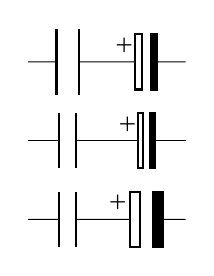
\begin{tikzpicture}
        \draw (0,1) to [C] ++(1,0) to [elko] ++(1,0);
        \ctikzset{capacitors/width=0.15, capacitors/height=0.5}
        \draw (0,0) to [C] ++(1,0) to [elko] ++(1,0);
        \tikzset{big elko/.style={elko=#1, capacitors/width=0.3}}
        \draw (0,-1) to [C] ++(1,0) to[big elko] ++(1,0);
    \end{tikzpicture}
\end{LTXexample}


\subsubsection{Inductors}

If the \texttt{cuteinductors} option is active (default behaviour), or the style \texttt{[cute inductors]} is used, the inductors are displayed as follows:
\begin{groupdesc}
    \ctikzset{inductor=cute}
    \circuitdescbip[cuteinductor]{L}{Inductor}{cute inductor}(midtap/90/0.1)
    \circuitdescbip[vcuteinductor]{vL}{Variable inductor}{variable cute inductor}(wiper/180/0.3, tip/0/0.3)
    \circuitdescbip[scuteinductor]{sL}{Inductive sensor}{cute inductive sensor}(label/0/0.3, wiper/180/0.3, tip/0/0.3)
\end{groupdesc}

If the \texttt{americaninductors} option is active (or the style \texttt{[american inductors]} is used), the inductors are displayed as follows:
\begin{groupdesc}
    \ctikzset{inductor=american}
    \circuitdescbip[americaninductor]{L}{Inductor}{american inductor}(midtap/90/0.3)
    \circuitdescbip[vamericaninductor]{vL}{Variable inductor}{variable american inductor}(core west/135/0.1, core east/45/0.1, wiper/180/0.3, tip/90/0.1)
    \circuitdescbip[samericaninductor]{sL}{Inductive sensor}{american inductive sensor}(label/0/0.3, wiper/180/0.3, tip/0/0.3)
\end{groupdesc}

Finally, if the \texttt{europeaninductors} option is active (or the style \texttt{[european inductors]} is used), the inductors are displayed as follows:
\begin{groupdesc}
    \ctikzset{inductor=european}
    \circuitdescbip[fullgeneric]{L}{Inductor}{european inductor}(midtap/90/0.1)
    \circuitdescbip[tfullgeneric]{vL}{Variable inductor}{variable european inductor}(wiper/180/0.3, tip/90/0.1,core west/135/0.1, core east/45/0.1)
    \circuitdescbip[sfullgeneric]{sL}{Inductive sensor}{european inductive sensor}(label/0/0.3, wiper/180/0.3, tip/0/0.3)
    \ctikzset{inductor=cute} % back to default
\end{groupdesc}

For historical reasons, \emph{chokes} come only in the \texttt{cute}. You can use the \texttt{core west} and \texttt{core east} anchors (see~\ref{sec:inductors-core-anchors}) to build your own core lines for the other inductors.

\begin{groupdesc}
    \circuitdescbip[cutechoke]{cute choke}{Choke}{}
\end{groupdesc}

\subsubsection{Inductors customizations}\label{sec:tweak-l}

You can change the scale of the inductors by setting the key \texttt{inductors/scale}  to something different from the default \texttt{1.0}. For thickness, you can use the same keys (applied to the \texttt{inductors} class) as for resistors in~\ref{sec:resistor-thickness}.

Variable inductors arrow tips follow the settings  of resistors, see section~\ref{sec:tunablearrows}.

You can change the width of these components (all the inductors together, unless you use style or scoping) by setting the key \texttt{inductors/width}  to something different from the default, which is  \texttt{0.8} for american and european inductors, and \texttt{0.6} for cute inductors.

Moreover, you can change the number of ``coils'' drawn by setting the key
\texttt{inductors/coils} (default value \texttt{5} for cute inductors and \texttt{4} for american ones). \textbf{Notice} that the minimum number of \texttt{coils} is \texttt{1} for american inductors, and \texttt{2} for cute ones.

\begin{LTXexample}[varwidth=true]
\begin{circuitikz}[
        longL/.style = {cute inductor, inductors/scale=0.75,
        inductors/width=1.6, inductors/coils=9}]
   \draw (0,1.5) to[L, l=$L$] ++(4,0);
   \draw (0,0) to[longL, l=$L$] ++(4,0);
   \ctikzset{inductors/scale=1.5, inductor=american}
   \draw (0,-1.5) to[L, l=$L$] ++(4,0);
\end{circuitikz}
\end{LTXexample}

\paragraph{Chokes} can have single and double lines, and can have the line thickness adjusted (the value is relative to the thickness of the inductor). In general, you should use the anchors (see~\ref{sec:inductors-core-anchors}) to add core lines to inductors.

\begin{LTXexample}[varwidth=true]
\begin{circuitikz}[american]
    \draw (0,0) to[cute choke] ++(3,0);
    \draw (0,-1) to[cute choke, twolineschoke] ++(3,0);

    \ctikzset{bipoles/cutechoke/cthick=2, twolineschoke}

    \draw (0,-2) to[cute choke] ++(3,0);
    \draw (0,-3) to[cute choke, onelinechoke] ++(3,0);
\end{circuitikz}
\end{LTXexample}


\subsubsection{Inductors anchors}

For inductive sensors, you have the same anchors than in the case of resistive sensors, see section~\ref{sec:sensors-anchors}.

\paragraph{Taps.}
Inductors have an additional anchor, called \texttt{midtap}, that connects to the center of the coil ``wire''. Notice that this anchor could be on one side or the other of the component, depending on the number of loops of the element; if you need a fixed position, you can use the geographical anchors.

\begin{LTXexample}[varwidth=true]
\begin{circuitikz}[
    loops/.style={circuitikz/inductors/coils=#1}]
\ctikzset{cute inductors}
\draw (0,2) to[L, loops=5, name=A] ++(2,0)
to[L, loops=6, name=B] ++(2,0);
\ctikzset{american inductors}
\draw (0,0) to[L, loops=5, name=C] ++(2,0)
to[L, loops=6, name=D] ++(2,0);
\foreach \i in {A, B, C, D}
  \node[circle, fill=red, inner sep=1pt] at (\i.midtap){};
\end{circuitikz}
\end{LTXexample}

\paragraph{Core anchors.}\label{sec:inductors-core-anchors}
Inductors have additional anchors to add core lines (for historical reasons, there is a \texttt{cute choke} component also, but to use inductors in the chosen style you'd better use these anchors). The anchors are called \texttt{core west} and \texttt{core east} and they are positioned at a distance that you can tweak with the \texttt{\textbackslash ctikzset} key \texttt{bipoles/inductors/core distance} (default \texttt{2pt}).

\begin{LTXexample}[varwidth]
    \begin{circuitikz}[]
        \ctikzset{american}
        \draw (0,3) to[L=$L$, name=myL] ++(2,0);
        \draw[thick] (myL.core west) -- (myL.core east);
        \ctikzset{cute inductors}
        \draw (0,1.5) to[L=$L$, name=myL] ++(2,0);
        \draw[densely dashed] (myL.core west) -- (myL.core east);
        \ctikzset{european, bipoles/inductors/core distance=4pt}
        \draw (0,0) to[L=$L$, name=myL, label distance=2pt] ++(2,0);
        \draw[thick, double] (myL.core west) -- (myL.core east);
    \end{circuitikz}
\end{LTXexample}

Notice that the core lines will \textbf{not} change the position of labels. You have to move them by hand if needed (or position them on the other side); see~\ref{sec:adjust-label-position}.

\paragraph{Dot anchors.}
Inductances also have ``dot'' anchors\footnote{proposed by Romano in a discussion by \href{https://github.com/circuitikz/circuitikz/issues/618}{GitHub user AndreaDiPietro92}},
to help positioning dots when specifying mutual inductance signs. The anchors are name \texttt{lr dot} (for lower right dot), \texttt{ur dot} (upper right) and so on:
\begin{quote}
    \showanchors{cuteinductorshape}{}(lr dot/-45/0.2, ur dot/45/0.2, ll dot/-135/0.2, ul dot/135/0.2)
    \quad
    \showanchors{cuteinductorshape}{}(ur dot/-60/0.3, ul dot/-120/0.3, core west/135/0.2, core east/45/0.2)
\end{quote}
and as you can see, you have to be careful if you use dot anchors and core anchors together.
You can change the position of the dots by changing the keys \texttt{bipoles/inductors/dot x distance} (default \texttt{4pt}), which represent how much the dot extends outside the component width, and the corresponding \texttt{dot y distance} (default \texttt{1pt}), which serves the same scope in the height direction.

\begin{LTXexample}[varwidth=true, basicstyle=\small\ttfamily]
\begin{circuitikz}[]
    \ctikzset{bipoles/inductors/.cd, dot x distance=3pt,
        dot y distance=0pt}
    \draw (0,2) to[L=$L_1$, name=l1] ++(3,0);
    \draw (0,0) to[L, l_=$L_2$, name=l2, inductors/width=1.4,
        inductors/coils=11] ++(3,0);
    \path (l1.ur dot) node[circ]{} (l2.ul dot) node[circ]{};
    \draw ([yshift=-0.2cm]l1.south)
        to[out=-45, in=45] node[right]{$M$}
        ([yshift=0.2cm]l2.north);
\end{circuitikz}
\end{LTXexample}

Notice that the position of the dot anchors does not coincide with the position of the dots in the transformers (see section~\ref{sec:transformers}), because there they depend on the size of the complete double-bipole more that on the size of the inductances.

\subsection{Diodes and such}

There are three basic styles for diodes: \texttt{empty} (fillable in color), \texttt{full} (completely filled with the draw color) and \texttt{stroke} (empty, but with a line across them).

You can switch between the styles setting the key \texttt{diode} (for example \verb|\ctikzset{diode=full}|  or \texttt{empty} or \texttt{stroke}, or with the styles \texttt{full diodes}, \texttt{empty diodes} and \texttt{stroke diodes}.


To use the default element, simply use the name shown for the empty diodes without the final ``o'' --- that is \texttt{D}, \texttt{sD}, and so on. The names shown in the following tables will draw the specified diode independently on the style chosen (that is, \texttt{leD*} is always a full LED diode).

\begin{framed}
The package options \texttt{fulldiode}, \texttt{strokediode}, and \texttt{emptydiode} (and the styles \texttt{[full diodes]}, \texttt{[stroke diodes]}, and \texttt{[empty diodes]}) define which shape will be used by abbreviated commands such that \texttt{D}, \texttt{sD}, \texttt{zD}, \texttt{zzD}, \texttt{tD}, \texttt{pD}, \texttt{leD}, \texttt{VC}, \texttt{Ty},\texttt{Tr} (no stroke symbol available!).
\end{framed}

\begin{groupdesc}
    \circuitdescbip*[emptydiode] {empty diode}{Empty diode}{Do}
    \circuitdescbip*[emptysdiode]{empty Schottky diode}{Empty Schottky diode}{sDo}
    \circuitdescbip*[emptyzdiode]{empty Zener diode}{Empty Zener diode}{zDo}
    \circuitdescbip*[emptyzzdiode]{empty ZZener diode}{Empty ZZener diode}{zzDo}
    \circuitdescbip*[emptytdiode]{empty tunnel diode}{Empty tunnel diode}{tDo}
    \circuitdescbip*[emptypdiode]{empty photodiode}{Empty photodiode}{pDo}(arrows/-30/0.3)
    \circuitdescbip*[emptylediode]{empty led}{Empty led}{leDo}(arrows/-30/0.3)
    \circuitdescbip*[emptylaserdiode]{empty laser diode}{Empty laser diode\footnotemark}{lasD}(arrows/-30/0.3)
		\footnotetext{Added by André Alves in \texttt{v1.4.4}}
    \circuitdescbip*[emptyvarcap]{empty varcap}{Empty varcap}{VCo}
    \circuitdescbip*[emptytvsdiode]{empty TVS diode}{Empty TVS diode, transorb\footnotemark}{tvsDo}
    \footnotetext{Transobs were suggested by \href{Anisio Braga}{https://tex.stackexchange.com/q/642219/38080}}
    \circuitdescbip*[emptyshdiode]{empty Shockley diode}{Empty Shockley diode\footnotemark}{shDo}
    \footnotetext{Shockley diodes were suggested by \href{@Dauph}{https://tex.stackexchange.com/q/646039/38080}}
    \circuitdescbip*[emptybidirectionaldiode]{empty bidirectionaldiode}{Empty bidirectionaldiode}{biDo}
    \circuitdescbip[fulldiode] {full diode}{Full diode}{D*}
    \circuitdescbip[fullsdiode]{full Schottky diode}{Full Schottky diode}{sD*}
    \circuitdescbip[fullzdiode]{full Zener diode}{Full Zener diode}{zD*}
    \circuitdescbip[fullzzdiode]{full ZZener diode}{Full ZZener diode}{zzD*}
    \circuitdescbip[fulltdiode]{full tunnel diode}{Full tunnel diode}{tD*}
    \circuitdescbip[fullpdiode]{full photodiode}{Full photodiode}{pD*}(arrows/-30/0.3)
    \circuitdescbip[fulllediode]{full led}{Full led}{leD*}(arrows/-30/0.3)
    \circuitdescbip[fulllaserdiode]{full laser diode}{Full laser diode}{lasD*}(arrows/-30/0.3)
    \circuitdescbip[fullvarcap]{full varcap}{Full varcap}{VC*}
    \circuitdescbip[fulltvsdiode]{full TVS diode}{Full TVS diode, transorb}{tvsD*}
    \circuitdescbip[fullshdiode]{full Shockley diode}{Full Shockley diode}{shD*}
    \circuitdescbip[fullbidirectionaldiode]{full bidirectionaldiode}{Full bidirectionaldiode}{biD*}
\end{groupdesc}

These shapes have no exact node-style counterpart, because the stroke line is built upon the empty variants:

\begin{groupdesc}
    \circuitdescbip*[emptydiode] {stroke diode}{Stroke diode}{D-}
    \circuitdescbip*[emptysdiode]{stroke Schottky diode}{Stroke Schottky diode}{sD-}
    \circuitdescbip*[emptyzdiode]{stroke Zener diode}{Stroke Zener diode}{zD-}
    \circuitdescbip*[emptyzzdiode]{stroke ZZener diode}{Stroke ZZener diode}{zzD-}
    \circuitdescbip*[emptytdiode]{stroke tunnel diode}{Stroke tunnel diode}{tD-}
    \circuitdescbip*[emptypdiode]{stroke photodiode}{Stroke photodiode}{pD-}(arrows/-30/0.3)
    \circuitdescbip*[emptylediode]{stroke led}{Stroke led}{leD-}(arrows/-30/0.3)
    \circuitdescbip*[emptylaserdiode]{stroke laser diode}{Stroke laser diode}{lasD-}(arrows/-30/0.3)
    \circuitdescbip*[emptyvarcap]{stroke varcap}{Stroke varcap}{VC-}
\end{groupdesc}

\subsubsection{Tripole-like diodes}\label{sec:othertrip} The following tripoles are entered with the usual command, of the form \texttt{to[Tr, \dots]}. In the following list you can see the traditional, or \texttt{legacy}, shape of the Thyristors-type devices.


\begin{groupdesc}
    \ctikzset{thyristor style=legacy}
    \circuitdescbip[fulldiode] {full diode}{Full diode}{D*}
    \circuitdescbip*[emptydiode] {stroke diode}{Stroke diode}{D-}
    \circuitdescbip*[emptytriac]{triac}{Standard triac (shape depends on package option)}{Tr}( G/0/0.3, anode/-90/0.2, cathode/-90/0.2)
    \circuitdescbip*[emptytriac]{empty triac}{Empty triac}{Tro}( gate/0/0.3 )
    \circuitdescbip[fulltriac]{full triac}{Full triac}{Tr*}
    \circuitdescbip*[emptythyristor]{thyristor}{Standard thyristor (shape depends on package option)}{Ty}( G/0/0.3, gate/45/0.3, anode/-90/0.2, cathode/-90/0.2)
    \circuitdescbip*[emptythyristor]{empty thyristor}{Empty thyristor}{Tyo}
    \circuitdescbip[fullthyristor]{full thyristor}{Full thyristor}{Ty*}
    \circuitdescbip*[emptythyristor]{stroke thyristor}{Stroke thyristor}{Ty-}
    \circuitdescbip*[emptyput]{put}{Standard Programmable Unipolar Transistor\footnotemark (shape depends on package option)}{PUT}( G/0/0.3, gate/45/0.3, anode/-90/0.2, cathode/-90/0.2)
    \footnotetext{This components, and the GTO family, has been suggested by \href{https://github.com/circuitikz/circuitikz/issues/522}{GitHub user JetherReis}.}
    \circuitdescbip*[emptyput]{empty put}{Empty PUT}{PUTo}
    \circuitdescbip[fullput]{full put}{Full PUT}{PUT*}
    \circuitdescbip*[emptyput]{stroke put}{Stroke PUT}{PUT-}
    \circuitdescbip*[emptygto]{gto}{Standard GTO (shape depends on package option)}{GTO}( G/0/0.3, gate/45/0.3, anode/-90/0.2, cathode/-90/0.2)
    \circuitdescbip*[emptygto]{empty gto}{Empty GTO}{GTOo}
    \circuitdescbip[fullgto]{full gto}{Full GTO}{GTO*}
    \circuitdescbip*[emptygto]{stroke gto}{Stroke GTO}{GTO-}
    \circuitdescbip*[emptygtobar]{gtobar}{Standard GTO with bar-type gate (shape depends on package option)}{GTOb}( G/0/0.3, gate/45/0.3, anode/-90/0.2, cathode/-90/0.2)
    \circuitdescbip*[emptygtobar]{empty gtobar}{Empty GTO, bar-type}{GTObo}
    \circuitdescbip[fullgtobar]{full gtobar}{Full GTO, bar-type}{GTOb*}
    \circuitdescbip*[emptygtobar]{stroke gtobar}{Stroke GTO, bar type}{GTOb-}
    \circuitdescbip*[emptyagtobar]{agtobar}{Standard GTO with bar-type gate on anode (shape depends on package option)}{aGTOb}( G/0/0.3, gate/45/0.3, anode/-90/0.2, cathode/-90/0.2)
    \circuitdescbip*[emptyagtobar]{empty agtobar}{Empty GTO, bar-type on anode}{aGTObo}
    \circuitdescbip[fullagtobar]{full agtobar}{Full GTO, bar-type on anode}{aGTOb*}
    \circuitdescbip*[emptyagtobar]{stroke agtobar}{Stroke GTO, bar-type on anode}{aGTOb-}
\end{groupdesc}

For basically stylistical reasons, there is a different, more compact, shape available for them, activated with the key \texttt{thyristor style=compact} (the default is \texttt{legacy}). All the devices above are present, we will show here just the automatic version for shortness.

\begin{groupdesc}
    \ctikzset{thyristor style=compact}
    \circuitdescbip*[emptytriac]{triac}{Standard triac (shape depends on package option)}{Tr}(G/0/0.3, anode/-90/0.2, cathode/-90/0.2)
    \circuitdescbip*[emptythyristor]{thyristor}{Standard thyristor (shape depends on package option)}{Ty}(G/0/0.3, gate/45/0.3, anode/-90/0.2, cathode/-90/0.2)
    \circuitdescbip*[emptyput]{put}{Standard Programmable Unipolar Transistor (shape depends on package option)}{PUT}( G/0/0.3, gate/45/0.3, anode/-90/0.2, cathode/-90/0.2)
    \circuitdescbip*[emptygto]{gto}{Standard gto (shape depends on package option)}{GTO}(G/0/0.3, gate/45/0.3, anode/-90/0.2, cathode/-90/0.2)
    \circuitdescbip*[emptygtobar]{gtobar}{Standard GTO  with a bar symbol on the gate (shape depends on package option)}{GTOb}( G/0/0.3, gate/45/0.3, anode/-90/0.2, cathode/-90/0.2)
    \circuitdescbip*[emptyagtobar]{agtobar}{Standard GTO with bar-type gate on anode (shape depends on package option)}{aGTOb}( G/0/0.3, gate/45/0.3, anode/-90/0.2, cathode/-90/0.2)
\end{groupdesc}

\subsubsection{Thyristors anchors and customization}

When inserting a thrystor, a triac or a potentiometer, one needs to refer to the third node-gate (\texttt{gate} or \texttt{G}) for the former two; wiper (\texttt{wiper} or \texttt{W}) for the latter one. This is done by giving a name to the bipole:
\label{bipole-naming}
\begin{LTXexample}[varwidth=true]
\begin{circuitikz} \draw
  (0,0) to[Tr, n=TRI] (2,0)
        to[pR, n=POT] (4,0);
  \draw[dashed] (TRI.G) -| (POT.wiper)
;\end{circuitikz}
\end{LTXexample}

As commented above, you can change the shape of these devices (globally or locally) setting the key \texttt{thyristor style=compact} (the default is \texttt{legacy}). Additionally, normally the plain \texttt{GTO} symbols come without the arrows, but you can add them using a syntax similar to the one explained in section~\ref{sec:tunablearrows} using the arrow group \texttt{gto gate}.

\begin{LTXexample}[varwidth=true]
    \begin{circuitikz}[]
        \ctikzset{thyristor style=compact}
        \draw (0,0) to[GTO=$G_1$] ++(0,-3);
        \ctikzset{gto gate end arrow=latexslim}
        \draw (2,0) to[GTO*=$G_2$, mirror] ++(0,-3);
        \draw (4,0) to[GTOb-=$G_2$, mirror] ++(0,-3);
    \end{circuitikz}
\end{LTXexample}

Notice that you can set both \texttt{gto gate end arrow} and \texttt{gto gate start arrow} --- choosing just one of the two you can decide the ``rotation'' direction of the symbol. There is little space though, so don't overdo it.

\subsubsection{Diode customizations}\label{sec:tweak-d}

You can change the scale of the diodes by setting the key \texttt{diodes/scale}  to something different from the default \texttt{1.0}. In Romano's opinion, diodes are somewhat big with the default style of the package, so a setting like \verb|\ctikzset{diode/scale=0.6}| is recommended.

\begin{LTXexample}[varwidth=true]
\begin{circuitikz}
   \draw (0,1) to[D, l=$D$] ++(2,0)
      node[npn, anchor=B]{};
   \ctikzset{diodes/scale=0.6}
   \draw (0,-1) to[D, l=$D$] ++(2,0)
      node[npn, anchor=B]{};
\end{circuitikz}
\end{LTXexample}

\paragraph{Optical devices arrows}\label{sec:opto-arrows} You can change the direction of the LEDs and photodiodes' arrows by using the binary keys \texttt{led arrows from cathode} and \texttt{pd arrows to cathode} (the default are \texttt{led arrows from anode} and \texttt{pd arrows to anode}), as you can see in the following example.

\begin{LTXexample}[varwidth=true]
    \begin{circuitikz}
        \ctikzset{led arrows from anode} % default
        \ctikzset{pd arrows to anode}    % default
        \ctikzset{full diodes}
        \draw (0,0) to[leD] ++(1.5,0) to[pD] ++(1.5,0);
        \ctikzset{stroke diodes}
        \draw (0,-1) to[leD] ++(1.5,0) to[pD] ++(1.5,0);
        \ctikzset{empty diodes}
        \draw (0,-2) to[leD] ++(1.5,0) to[pD] ++(1.5,0);

        \ctikzset{led arrows from cathode}
        \ctikzset{pd arrows to cathode}
        \ctikzset{full diodes}
        \draw (0,-4) to[leD] ++(1.5,0) to[pD] ++(1.5,0);
        \ctikzset{stroke diodes}
        \draw (0,-5) to[leD] ++(1.5,0) to[pD] ++(1.5,0);
        \ctikzset{empty diodes}
        \draw (0,-6) to[leD] ++(1.5,0) to[pD] ++(1.5,0);
    \end{circuitikz}
\end{LTXexample}

Since version \texttt{1.5.5}\footnote{Thanks to the idea by \href{https://github.com/circuitikz/circuitikz/issues/655}{Dr. Matthias Jung on GitHub}.}, you can change the arrows used for LEDs, photodiodes and laser diodes with the generic arrows options shown in~\ref{sec:tunablearrows}, using the name \texttt{opto}, like in the following (overdone) example. Normally you want just to change the \texttt{end arrow}\dots

As you can see, you can also have the option to globally change the color, relative thickness, and dash pattern  by setting keys with the \verb!\ctikzset! command (or, like in the following example, directly in the node instantiation) under the \texttt{opto arrows} hierarchy. The available keys are:

\begin{center}
    \begin{tabular}{>{\ttfamily}l>{\ttfamily}lp{0.5\linewidth}}
        \toprule
     parameter &  default & description  \\
     \midrule
     relative thickness & 1.0 & multiply the class thickness \\
     color & default & stroke color: \texttt{default} is the same as the component \\
     dash & default & dash pattern: \texttt{default} means not to change the setting for the component; \texttt{none} means unbroken line; every other input is a dash pattern.\footnotemark \\
        \bottomrule
    \end{tabular}
    \footnotetext{Follows the syntax of the pattern sequence \texttt{\textbackslash pgfsetdash} --- see \TikZ{} manual for details; phase is always zero. Basically you pass pairs of dash-length -- blank-length dimensions, see the examples.}
\end{center}

\begin{LTXexample}[varwidth=true, basicstyle=\small\ttfamily]
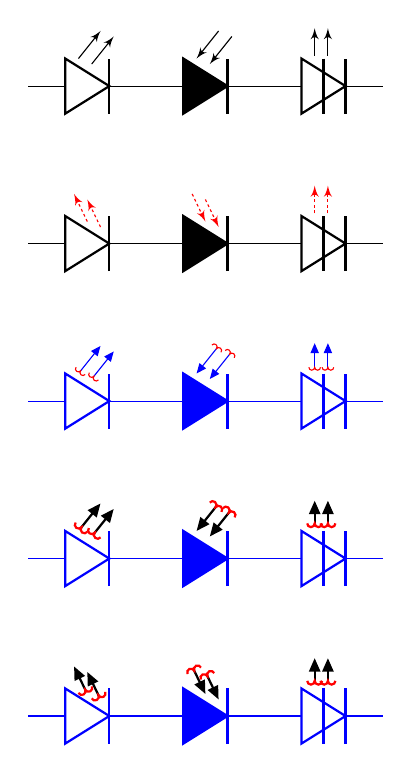
\begin{tikzpicture}
\newcommand{\optos}{%
    to[leD] ++(1.5,0) to[pD*] ++(1.5,0)
    to[lasD] ++(1.5,0)}
\begin{scope}
    \draw (0,2) \optos;
    \ctikzset{led arrows from cathode}
    \ctikzset{pd arrows to cathode}
    \ctikzset{opto arrows/.cd, color=red,
        dash={{1pt}{1pt}}}
    \draw (0,0) \optos;
\end{scope}
\begin{scope}[color=blue, yshift=-6cm]
    \ctikzset{opto end arrow={Triangle[angle'=45]}}
    \ctikzset{opto start arrow={Hooks[red]}}
    \draw (0,4) \optos;
    \ctikzset{opto arrows/color=black}
    \ctikzset{opto arrows/relative thickness=2}
    \draw (0,2) \optos;
    \ctikzset{led arrows from cathode}
    \ctikzset{pd arrows to cathode}
    \draw (0,0) \optos;
\end{scope}
\end{tikzpicture}
\end{LTXexample}


\subsection{Sources and generators}

Notice that source and generators are divided in three classes that can be styled independently: traditional battery symbols (class \texttt{batteries}), independent generators (class \texttt{sources}) and dependent generators (class \texttt{csources}). This is because they are often treated differently, and so you can choose to, for example, fill the dependent sources but not the independent ones.

\subsubsection{Batteries}
\begin{groupdesc}
    \circuitdescbip{battery}{Battery}{}
    \circuitdescbip{battery1}{Single battery cell}{}
    \circuitdescbip{battery2}{Single battery cell}{}
    \circuitdescbip{baertty}{Randall Munroe's baertty\footnotemark}{}
    \footnotetext{\href{https://xkcd.com/2818}{Mandatory xkcd}}
\end{groupdesc}

\subsubsection{Stationary sources}
\begin{groupdesc}
    \circuitdescbip*[vsource]{european voltage source}{Voltage source (european style)}{vsource}
    \circuitdescbip*[vsourceC]{cute european voltage source}{Voltage source (cute european style)}{vsourceC, ceV}
    \circuitdescbip*[vsourceAM]{american voltage source}{Voltage source (american style)}{vsourceAM}
    \circuitdescbip*[isource]{european current source}{Current source (european style)}{isource}
    \circuitdescbip*[isourceC]{cute european current source}{Current source (cute european style)}{isourceC, ceI}
    \circuitdescbip*[isourceAM]{american current source}{Current source (american style)}{isourceAM}
\end{groupdesc}

\begin{framed}
If (default behavior) \texttt{europeancurrents} option is active (or the style \texttt{[european currents]} is used), the shorthands \texttt{current source}, \texttt{isource}, and \texttt{I} are equivalent to \texttt{european current source}. Otherwise, if \texttt{americancurrents} option is active (or the style \texttt{[american currents]} is used) they are equivalent to \texttt{american current source}.

Similarly, if (default behavior) \texttt{europeanvoltages} option is active (or the style \texttt{[european voltages]} is used), the shorthands \texttt{voltage source}, \texttt{vsource}, and \texttt{V} are equivalent to \texttt{european voltage source}. Otherwise, if \texttt{americanvoltages} option is active (or the style \texttt{[american voltages]} is used) they are equivalent to \texttt{american voltage source}.
\end{framed}


\subsubsection{Sinusoidal sources}\label{sec:sinusoidal-vi} These two are basically the same symbol; to distinguish among them, you have to add a label, which will be a voltage or a current. Another option would be to configure the \texttt{sinusoidal current source} as an open shape using \texttt{\textbackslash ctikzset\string{bipoles/isourcesin/angle=80\string}} similar to the \texttt{dcisource} in section~\ref{sec:dc-sources}.

\begin{groupdesc}
    \circuitdescbip*[vsourcesin]{sinusoidal voltage source}{Sinusoidal voltage source}{vsourcesin, sV}
    \circuitdescbip*[isourcesin]{sinusoidal current source}{Sinusoidal current source\footnotemark}{isourcesin, sI}
      \footnotetext{The configurable open shape of the \texttt{sinusoidal current source} has been added by \href{https://github.com/circuitikz/circuitikz/pull/737}{Maximilian Martin}}.
\end{groupdesc}

\begin{LTXexample}[varwidth=true]
\begin{circuitikz}[american]
   \draw (0,2) to[sV=$V$] ++(3,0);
   \draw (0,1) to[sI=$I$] ++(3,0);
   \ctikzset{bipoles/isourcesin/angle=80}
   \draw (0,0) to[sI] ++(3,0);
\end{circuitikz}
\end{LTXexample}

\subsubsection{Controlled sources}
\begin{groupdesc}
    \circuitdescbip*[cvsource]{european controlled voltage source}{Controlled voltage source (european style)}{cvsource}
    \circuitdescbip*[cvsourceC]{cute european controlled voltage source}{Voltage source (cute european style)}{cvsourceC, cceV}
    \circuitdescbip*[cvsourceAM]{american controlled voltage source}{Controlled voltage source (american style)}{cvsourceAM}
    \circuitdescbip*[cisource]{european controlled current source}{Controlled current source (european style)}{cisource}
    \circuitdescbip*[cisourceC]{cute european controlled current source}{Current source (cute european style)}{cisourceC, cceI}
    \circuitdescbip*[cisourceAM]{american controlled current source}{Controlled current source (american style)}{cisourceAM}
    \circuitdescbip*[ecsource]{empty controlled source}{Empty controlled source}{ecsource}
\end{groupdesc}

\begin{framed}
If (default behaviur) \texttt{europeancurrents} option is active (or the style \texttt{[european currents]} is used), the shorthands \texttt{controlled current source}, \texttt{cisource}, and \texttt{cI} are equivalent to \texttt{european controlled current source}. Otherwise, if \texttt{americancurrents} option is active (or the style \texttt{[american currents]} is used) they are equivalent to \texttt{american controlled current source}.

Similarly, if (default behaviur) \texttt{europeanvoltages} option is active (or the style \texttt{[european voltages]} is used), the shorthands \texttt{controlled voltage source}, \texttt{cvsource}, and \texttt{cV} are equivalent to \texttt{european controlled voltage source}. Otherwise, if \texttt{americanvoltages} option is active (or the style \texttt{[american voltages]} is used) they are equivalent to \texttt{american controlled voltage source}.
\end{framed}

The following two behave like the corresponding independent sources, see section~\ref{sec:sinusoidal-vi}.

\begin{groupdesc}
    \circuitdescbip*[cvsourcesin]{controlled sinusoidal voltage source}{Controlled sinusoidal voltage source}{controlled vsourcesin, cvsourcesin, csV}
    \circuitdescbip*[cisourcesin]{controlled sinusoidal current source}{Controlled sinusoidal current source}{controlled isourcesin, cisourcesin, csI}
\end{groupdesc}



\subsubsection{Noise sources}

In this case, the ``direction''  of the source is undefined. Noise sources are filled in gray by default, but if you choose the dashed style, they become fillable.

\begin{groupdesc}
    \circuitdescbip[vsourceN]{noise voltage source}{Sinusoidal voltage source}{vsourceN, nV}
    \circuitdescbip[isourceN]{noise current source}{Sinusoidal current source}{isourceN, nI}
\end{groupdesc}

You can change the fill color with the key \texttt{circuitikz/bipoles/noise sources/fillcolor}:
\begin{LTXexample}[varwidth=true]
\begin{circuitikz}
    \draw(0,0) to [nV, l=$e_n$] ++(2,0);
    \draw(0,-2) to [nI, l=$i_n$] ++(2,0);
    \begin{scope}[circuitikz/bipoles/noise sources/fillcolor=red!50]
        \draw(3,0) to [nV, l=$e_n$] ++(2,0);
        \draw(3,-2) to [nI, l=$i_n$] ++(2,0);
    \end{scope}
\end{circuitikz}
\end{LTXexample}

If you prefer a patterned noise generator (similar to the one you draw by hand) you can use the fake color \texttt{dashed}:
\begin{LTXexample}[varwidth=true]
\begin{circuitikz}
    \draw(0,0) to [nV, l=$e_n$] ++(2,0);
    \draw(0,-2) to [nI, l=$i_n$] ++(2,0);
    \begin{scope}[circuitikz/bipoles/noise sources/fillcolor=dashed]
        \draw(3,0) to [nV, l=$e_n$] ++(2,0);
        \draw(3,-2) to [nI, l=$i_n$] ++(2,0);
    \end{scope}
\end{circuitikz}
\end{LTXexample}

Notice that if you choose the dashed style, the noise sources are fillable:
\begin{LTXexample}[varwidth=true]
\begin{circuitikz}
    \ctikzset{bipoles/noise sources/fillcolor=dashed}
    \draw(0,0) to [nV, l=$e_n$] ++(2,0);
    \draw(0,-2) to [nI, l=$i_n$] ++(2,0);
    \begin{scope}
        \draw(3,0) to [nV, l=$e_n$, fill=yellow!50!red] ++(2,0);
        \draw(3,-2) to [nI, l=$i_n$, fill=blue!50!white] ++(2,0);
    \end{scope}
\end{circuitikz}
\end{LTXexample}

\subsubsection{Special sources}
\begin{groupdesc}
    \circuitdescbip*[vsourcesquare]{square voltage source}{Square voltage source}{vsourcesquare, sqV}
    \circuitdescbip*{vsourcetri}{Triangle voltage source}{tV}
    \circuitdescbip*{esource}{Empty voltage source}{}
    \circuitdescbip*{pvsource}{Photovoltaic-voltage source}{}
    \circuitdescbip*{pvmodule}{Photovoltaic module source\footnotemark}{}
		\footnotetext{Added by André Alves in \texttt{v1.3.5}}
    \circuitdescbip*[oosource]{ioosource}{Double Zero style current source}{}
    \circuitdescbip*[oosource]{voosource}{Double Zero style voltage source}{}
    \circuitdescbip*[oosourcetrans]{oosourcetrans}{transformer source\footnotemark}{}(centerprim/90/0.3, centersec/-90/0.3)
        \footnotetext{The \texttt{oosourcetrans} and \texttt{ooosource} components have been added by \href{https://github.com/circuitikz/circuitikz/pull/397}{user \texttt{@olfline} on GitHub}}.
    \begingroup
        \ctikzset{sources/scale=1.5}
        \circuitdescbip*[ooosource]{ooosource}{transformer with three windings\footnotemark}{}(left/175/0.2, right/5/0.7, prim1/130/.2, prim2/-130/.2, sec1/35/.2, sec2/60/.2, sec3/90/.2, tert1/0/.2, tert2/-45/.2, tert3/-90/.2, centerprim/92/0.8, centersec/35/0.9, centertert/-35/0.8)
        \footnotetext{The component here is scaled up 1.5 times to better show the anchors.}
    \endgroup
\end{groupdesc}

The transformer shapes vector group options can be specified for the primary (\texttt{prim=\emph{value}}), the secondary (\texttt{sec=\emph{value}}) and tertiary (\texttt{tert=\emph{value}}) three-phase vector groups: the value can be one of \texttt{delta}, \texttt{wye} and \texttt{zig}.

\begin{LTXexample}[varwidth=true]
\begin{circuitikz}
    \draw (0,0) to[oosourcetrans, prim=zig, sec=delta, o-] ++(2,0)
    to[oosourcetrans, prim=delta, sec=wye,-o] ++(0,-2)
    to[ooosource, prim=wye, sec=zig, tert=delta] (0,0);
\end{circuitikz}
\end{LTXexample}

These two ``sources'' have additional anchors that reach the center of the symbol;\footnote{Suggested by \href{https://github.com/circuitikz/circuitikz/issues/725}{user @lapreindl on GitHub}.} they are used sometimes to add a (symbolic) connection there, like for example a ground connection.

\begin{LTXexample}[varwidth=true]
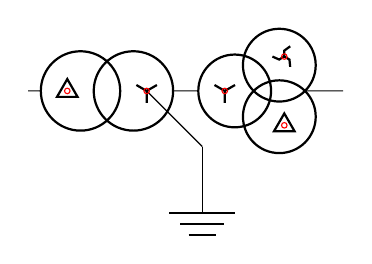
\begin{tikzpicture}[european, scale=2, transform shape,
    smalldot/.style={draw, circle,red, inner sep=0.2pt}]
    \draw (0,0) to[oosourcetrans, name=A,
            prim=delta, sec=wye] ++(1,0)
        to[ooosource, name=B, prim=wye, sec=zig,
            tert=delta] ++(1,0)
        (A.symbolsec) -- ++(-45:0.5) node[ground]{};
    \node [smalldot] at (A.symbolprim) {};
    \node [smalldot] at (A.symbolsec) {};
    \node [smalldot] at (B.symbolprim) {};
    \node [smalldot] at (B.symbolsec) {};
    \node [smalldot] at (B.symboltert) {};
\end{tikzpicture}
\end{LTXexample}

\subsubsection{Nullator and norator}

These are special elements used in some approaches to model ideal amplifiers\footnote{See \href{https://en.m.wikipedia.org/wiki/Nullor}{the Wikipedia article}; suggested by \href{https://github.com/circuitikz/circuitikz/issues/615}{user atticus-sullivan on GitHub}.}.

\begin{groupdesc}
\circuitdescbip*{nullator}{Nullator element (virtual short circuit; forces V and I to zero)}{}
\circuitdescbip*{norator}{Norator element (admits any combination of V and I)}{}
\end{groupdesc}

They are in the \texttt{sources} class, but they are not treated like sources in the labeling sense (they have both \texttt{bipoles/is voltage=false} and \texttt{bipoles/is current=false}, see~\ref{sec:source-vif}).

\begin{LTXexample}[varwidth=true]
\begin{circuitikz}[american]
    \draw (0,0) node[ground](GND){}
        to [I,l=$i_s$,invert]
        ++(0,2.5) -- ++(1.5,0) coordinate(up)
        to[nullator, v=0, i=0, name=A]
        (up|-GND) node[ground]{};
    \draw (up) to[R, *-*] ++(2,0) coordinate(out)
        to[norator, v^=$v_o$]
        (out|-GND) node[ground]{};
\end{circuitikz}
\end{LTXexample}

The symbol shapes used here seems to be the most common in publications; if you prefer the shapes from the Wikipedia article, you can use the following definitions:

\begin{LTXexample}[varwidth=true]
\tikzset{noratorW/.style={voosource,
		bipoles/oosource/circlesize=0.5,
		bipoles/oosource/circleoffset=0.5},
	nullatorW/.style={esource, sources/scale=0.5}}
\begin{tikzpicture}
    \draw (0,0) to[nullatorW] ++(2,0) to[noratorW] ++(0, -2);
\end{tikzpicture}
\end{LTXexample}

\subsubsection{DC sources}\label{sec:dc-sources}
\begin{groupdesc}
    \circuitdescbip*{dcvsource}{DC voltage source}{}
    \circuitdescbip*{dcisource}{DC current source}{}
\end{groupdesc}

The size of the broken part of the DC current source is configurable by changing the value of \texttt{bipoles/dcisource/angle} (default \texttt{80}); values must be between 0 (no circle at all, probably not useful) and 90 (full circle, again not useful).
\begin{LTXexample}[varwidth=true]
\begin{circuitikz}
    \draw (0,0) to[dcvsource] ++(2,0)
    to [dcisource, fill=yellow] ++(2,0) ;
    \ctikzset{bipoles/dcisource/angle=45}
    \draw (0,-2) to[dcvsource] ++(2,0)
    to [dcisource, fill=yellow] ++(2,0) ;
\end{circuitikz}
\end{LTXexample}

\subsubsection{Sources customizations}\label{sec:tweak-sources}

\paragraph{Size.}
You can change the scale of the batteries by setting the key \texttt{batteries/scale}, for the controlled (dependent) sources with \texttt{csources/scale}, and for all the other independent sources and generators with \texttt{sources/scale}, to something different from the default \texttt{1.0}.

Notice that the size of the double-circle sources (and of the triple-circle one) are tuned so that the full source occupy more or less the same horizontal space than one of the single-circle one; as a consequence, the circles are much smaller. If you want to have the same circle radius, you have to scale (locally!) those sources by one factor that is \texttt{1.5384} ($1/0.65$) for \texttt{oosource}, \texttt{1.6667} ($1/0.6$) for \texttt{oosourcetrans}, and \texttt{1.8182} ($1/0.55$) for \texttt{ooosource}.

\begin{LTXexample}[varwidth=true]
\begin{circuitikz}
    \draw[color=red] (0,0) to[esource] ++(3,0);
    \draw (0,0) to[oosourcetrans, prim=delta, sec=wye,
        sources/scale=1.667] ++(3,0);
\end{circuitikz}
\end{LTXexample}

\paragraph{Waveform symbols.}
Internal symbols of sinusoidal, triangular and square sources are drawn with the same line thickness as the component by default. You can modify this by setting the key \texttt{sources/symbols/thickness} for independent sources and the corresponding \texttt{csource/...} for dependent ones. The value used here is relative to the component (i.e. the circle) value.

Normally the symbol is oriented in the same direction as the line, and rotate rigidly with the component; you can change this orientation using the key \texttt{sources/symbols/rotate} or \texttt{csource/...}. The default value is \texttt{90} which correspond to the ``line'' direction (remember, path components are defined as horizontal ones).
If instead of an angle value you use \texttt{auto}, the symbol will be rotated so that the waveform is always vertical, similar to what happens in instruments:

\begin{LTXexample}[varwidth=true]
\begin{circuitikz}
    \draw (0,1) to[sqV] ++(3,0)
        to[sqV] ++(1,-1)
        to[sqV] ++(0,-3);
    \ctikzset{sources/symbol/rotate=auto}
    \ctikzset{sources/symbol/rotate=auto, sources/symbol/thickness=3}
    \draw[color=red] (0,0) to[sqV] ++(3,0)
        to[sqV] ++(0,-3)
        to[sqV] (0,0);
\end{circuitikz}
\end{LTXexample}


\paragraph{Polarity symbols.}
The symbols drawn into the \texttt{american voltage source}\footnote{Since version \texttt{1.1.0}, thanks to the suggestions and discussion
\href{https://tex.stackexchange.com/questions/538723/circuitikz-what-should-i-do-to-put-the-and-on-the-appropriate-places-like-t}{in this TeX.SX question}.} can be changed by using the \verb|\ctikzset|  keys \texttt{bipoles/vsourceam/inner plus} and \texttt{.../inner minus} (by default they are \verb|$+$| and \verb|$\vphantom{+}-$| respectively, in the current font), and move them nearer of farther away by twiddling \texttt{bipoles/vsourceam/margin} (default \texttt{0.7}, less means nearer). The reason of the \verb|\vphantom| can be found in section~\ref{sec:american-voltage-custom}.

You can do the same with the \texttt{american controlled voltage sources}, substituting \texttt{cvsourceam} to \texttt{vsourceam} (notice the initial ``\texttt{c}'').

\begin{LTXexample}[varwidth=true]
\begin{circuitikz}[american]
   \ctikzset{bipoles/vsourceam/inner plus={\tiny $+$}}
   \ctikzset{bipoles/vsourceam/inner minus={\tiny $-$}}
   \draw (0,0) to[V, l_=$V$] ++(0,3)
   to[R=\SI{5}{\ohm}] ++(3,0)
   to[V, invert,
   bipoles/vsourceam/inner plus={\color{red}\tiny $\oplus$},
   bipoles/vsourceam/inner minus={\color{blue}\tiny $\ominus$},
   bipoles/vsourceam/margin=0.5]
   ++(0,-3) to[short, -*] (0,0) node[ground]{};
\end{circuitikz}
\end{LTXexample}

\paragraph{Three-phase symbols.}
The three-phase symbols \texttt{delta}, \texttt{wye}, and \texttt{zig} follows the line thickness exactly as
the waveform ones (see above). Additionally, you can scale them up and down by changing the value of the keys
\texttt{sources/symbol/delta scale}, \texttt{.../wye scale}, and \texttt{.../zig scale} (default \texttt{1}).

\begin{LTXexample}[varwidth=true]
\begin{circuitikz}[scale=1.8, transform shape]
    \tikzset{myoosource/.style={ooosource,
        prim=wye, sec=delta, tert=zig,
        }}
    \draw (0,2) to[myoosource] ++(2,0);
    \ctikzset{%
        sources/symbol/thickness=0.5,
        sources/symbol/delta scale=1.2,
        sources/symbol/wye scale=1.4,
        sources/symbol/zig scale=1.3,
    }
    \draw (0,0) to[myoosource] ++(2,0);
\end{circuitikz}
\end{LTXexample}

\subsubsection{Source borders}

Unfortunately, the border of the sources is only easily accessed if some anchor is provided.
The border anchors of the shapes are not tight on them (see section~\ref{sec:bipoles-border-anchors}), which is not easily changeable, given that the algorithm that positions the labels depends on it.

On the other hand, \TikZ{} powerful partway coordinate calculation (around section 13.5.3 of the manual) makes it possible to easily identify points on a circle if the center and one point of the circle are known, as you can see in the following example.

\begin{LTXexample}[varwidth=true, basicstyle=\small\ttfamily]
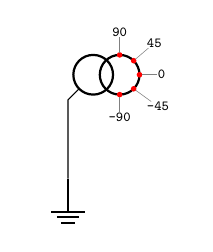
\begin{tikzpicture}[]
    \path (0,0) to[oosourcetrans, name=T, ]++(2,0);
    % Use partway modifiers to reach a point on the left circle
    \draw ($(T.centerprim)!1!45:(T.left)$) -- ++(-135:0.2)
        -- ++(0,-1) node[ground]{};
    \begin{scope}[font=\tiny\ttfamily, pin distance=2mm, inner sep=0pt]
        \foreach \a in {-90,-45,...,90}
            \node [circ, scale=0.5, pin=\a:\a, color=red] at
                ($(T.centersec)!1!\a:(T.right)$){};
    \end{scope}
\end{tikzpicture}
\end{LTXexample}

A similar approach can be used for dependent sources. Just remember that the anchors move (rotate) together with the component.

\begin{LTXexample}[varwidth=true, basicstyle=\small\ttfamily]
    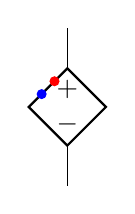
\begin{tikzpicture}[american]
        \draw (0,0) to [cvsource, name=S] ++(0,2);
        \node [circ,red] at ($(S.e)!0.3333!(S.n)$) {};
        \node [circ,blue] at ($(S.e)!0.6666!(S.n)$) {};
    \end{tikzpicture}
\end{LTXexample}


\subsection{Instruments}
\begin{groupdesc}
    \circuitdescbip*{ammeter}{Ammeter}{}
    \circuitdescbip*{voltmeter}{Voltmeter}{}
    \circuitdescbip*{ohmmeter}{Ohmmeter}{}
    \circuitdescbip*{rmeter}{Round meter (use \texttt{t=...} for the symbol)}{}(left/135/0.2, right/45/0.2, center/-90/0.3)
    \circuitdescbip*{rmeterwa}{Round meter with arrow (use \texttt{t=...} for the symbol)}{}(left/135/0.2, right/45/0.2, center/-90/0.3)
    \circuitdescbip*{smeter}{Square meter (use \texttt{t=...} for the symbol)}{}(left/135/0.2, right/45/0.2, center/-90/0.3, in 1/-135/.5, in 2/-45/.5)
    \circuitdescbip*{qiprobe}{QUCS-style current probe}{}(left/135/0.2, right/45/0.2, center/-90/0.3)
    \circuitdescbip*{qvprobe}{QUCS-style voltage probe}{}(left/135/0.2, right/45/0.2, center/-90/0.3)
    \circuitdescbip*{qpprobe}{QUCS-style power probe}{}(left/135/0.2, right/45/0.2, center/-90/0.3, v+/-135/.5, v-/-45/.5)
    \circuitdescbip*[oscope]{oscope}{Oscilloscope\footnotemark}{}(left/135/0.2, right/45/0.2,
    in 1/-135/0.4, in 2/-45/0.4)
    \footnotetext{Suggested by \texttt{@nobrl} on GitHub}
    \circuitdescbip{iloop}{Current loop (symbolic)}{}(left/135/0.2, right/45/0.2, center/-90/0.3, i/30/0.4)
    \circuitdescbip{iloop2}{Current loop (real)}{}(left/135/0.2, right/-45/0.2, center/-90/0.3, i+/135/0.4, i-/45/0.4)
\end{groupdesc}

\subsubsection{Instruments customizations}\label{sec:tweak-instruments}

You can change the scale of all the instruments (including the current loops) by setting the key \texttt{instruments/scale} to something different from the default \texttt{1.0}.

\paragraph{Oscilloscope waveform.} You can change the waveform shown in the oscilloscope ``screen''\footnote{Suggested by \href{https://tex.stackexchange.com/q/595062/38080}{Mario Tafur on TeX.SX}}. To change it, you just set the key \texttt{bipoles/oscope/waveform} to one of the available shape. You have available the shapes in the following list (the default is \texttt{ramps}):

\begin{LTXexample}[pos=t, basicstyle=\small\ttfamily]
\begin{circuitikz}
    \foreach [count=\i] \wvf in {ramps, sin, square, triangle, lissajous, zero, none} {
        \ctikzset{bipoles/oscope/waveform=\wvf}
        \draw ({2*\i},1.4) node[oscopeshape](O){}
              ({2*\i},0.65) node[anchor=base]{\texttt{\wvf}};
    }
    \ctikzset{bipoles/oscope/width=1.0}
    \foreach [count=\i] \wvf in {ramps, sin, square, triangle, lissajous, zero, none} {
        \ctikzset{bipoles/oscope/waveform=\wvf}
        \draw ({2*\i},0) node[oscopeshape]{};
    }
\end{circuitikz}
\end{LTXexample}

If you want more or different shapes, you can define your owns, but you have to use low-level \texttt{pgf} commands (see part IX, ``The Basic Layer'', in the PGF/\TikZ{} manual). The code is executed into a \verb|\pgfscope| \dots \verb|\endpgfscope| environment, and it must use the path built with a \verb|\pgfusepath|. The coordinates have been scaled so that the external box of the scope is a rectangle between \texttt{(-1cm, -1cm)} and \texttt{(1cm, 1cm)}; the oscilloscope grid is fixed and painted between \texttt{(-0.75cm, -0.5cm)} and \texttt{(0,75cm, 0.5cm)}. If you stretch the scope with the \texttt{\dots width} or \texttt{\dots height} keys, the drawing will be stretched too.

\begin{LTXexample}[varwidth=t, basicstyle=\small\ttfamily]
    \ctikzset{%
    bipoles/oscope/waveform/mywave/.code={%
        \pgfsetcolor{red}
        \pgfpathmoveto{\pgfpoint{-.75cm}{-.5cm}}
        \pgfpathlineto{\pgfpoint{.75cm}{.5cm}}
        \pgfusepath{draw}
        \pgfsetcolor{green}
        \pgfpathmoveto{\pgfpoint{-.75cm}{.5cm}}
        \pgfpathlineto{\pgfpoint{.75cm}{-.5cm}}
        \pgfusepath{draw}
    }}
    \begin{circuitikz}
        \ctikzset{bipoles/oscope/waveform=mywave}
        \draw (0,0) node[oscopeshape]{};
    \end{circuitikz}
\end{LTXexample}



\subsubsection{Rotation-invariant elements}

The \texttt{oscope} element will not rotate the ``graph'' shown with the component:

\begin{LTXexample}[varwidth=true]
\begin{circuitikz}
    \foreach \a in {0,45,...,350} {
        \draw (0,0) to[oscope] (\a:3);
    }
\end{circuitikz}
\end{LTXexample}

The \texttt{rmeter}, \texttt{rmaterwa}, and \texttt{smeter} have the same behavior.

However, if you prefer that the \texttt{oscope}, \texttt{rmeter}, \texttt{smeter}  and \texttt{rmeterwa} instruments rotate the text or the diagram,
you can use the key or style \texttt{rotated instruments} (the default style is \texttt{straight instruments}).

\begin{LTXexample}[varwidth=true]
    \begin{circuitikz}[scale=0.8, transform shape]
    \ctikzset{rotated instruments} % new default
    \draw (0,0) to[oscope] ++(0:3);
    \draw (0,0) to[oscope] ++(60:3);
    \draw (0,0) to[rmeter, t=A] ++(120:3);
    % local override
    \draw (0,0) to[rmeterwa, t=A, straight instruments] ++(180:3);
    \ctikzset{straight instruments} % back to default
    \draw (0,0) to[rmeterwa, t=A] ++(240:3);
    % local override
    \draw (0,0) to[smeter, t=A, rotated instruments] ++(300:3);
\end{circuitikz}
\end{LTXexample}



\subsubsection{Instruments as node elements}

The node-style usage of the \texttt{oscope} is also interesting, using the additional \texttt{in 1} and \texttt{in 2} anchors; notice that in this case you can use the text content of the node to put labels above it.
Moreover, you can change the size of the oscilloscope by changing \texttt{bipoles/oscope/width} and \texttt{bipoles/oscope/height} keys (which both default to 0.6).

\begin{LTXexample}[varwidth=true]
\begin{circuitikz}
    \draw (0,1)
        to[oscope=$C_1$, fill=green!20!gray, name=O1] ++(2,0);
    \path (O1.right)
        node[ground, scale=0.5, below right=4pt]{};
    \ctikzset{bipoles/oscope/width=1.0}
    \draw (1,-1)
        node[oscopeshape, fill=yellow!20!orange](O2){$C_2$};
    \draw (O2.in 2) to[short, *-] ++(0,-0.5) node[ground]{};
    \draw (O2.in 1) to[short, *-] ++(0,-0.5)
           -- ++(-1,0) node[currarrow, xscale=-1]{};
\end{circuitikz}
\end{LTXexample}

\subsubsection{Measuring voltage and currents, multiple ways}

This is the classical (legacy) option, with the \texttt{voltmeter} and \texttt{ammeter}. The problem is that elements are intrinsically horizontal, so they look funny if put in vertically.

\begin{LTXexample}[varwidth=true]
\begin{circuitikz}
    \draw (0,0) -- ++(1,0) to[R] ++(2,0)
    to [ammeter] ++(0,-2) node[ground]{};
    \draw (1,0) to[voltmeter] ++(0,-2)
    node[ground]{};
\end{circuitikz}
\end{LTXexample}

So the solution is often changing the structure to keep the meters in horizontal position.

\begin{LTXexample}[varwidth=true]
\begin{circuitikz}
    \draw (0,0) -- ++(1,0) to[R] ++(2,0)
    to [ammeter] ++(2,0) --
    ++(0,-1) node[ground]{};
    \draw (1,0) -- (1,1) to[voltmeter]
    ++(2,0) node[ground]{};
\end{circuitikz}
\end{LTXexample}

Since version 0.9.0 you have more options for the measuring instruments. You can use the generic \texttt{rmeterwa} (round meter with arrow), to which you can specify the internal symbol with the option \texttt{t=...} (and is fillable).

\begin{LTXexample}[varwidth=true]
\begin{circuitikz}[american]
    \draw (0,0) -- ++(1,0) to[R] ++(2,0)
    to [rmeterwa, t=A, i=$i$] ++(0,-2) node[ground]{};
    \draw (1,0) to[rmeterwa, t=V, v=$v$] ++(0,-2)
    node[ground]{};
\end{circuitikz}
\end{LTXexample}

This kind of component will keep the symbol horizontal, whatever the orientation:

\begin{LTXexample}[varwidth=true]
\begin{circuitikz}[american]
    \draw (0,0) -- ++(1,0) to[R] ++(2,0)
    to [rmeterwa, t=A, i=$i$] ++(2,0) --
    ++(0,-1) node[ground]{};
    \draw (1,0) -- (1,1) to[rmeterwa, t=V, v^=$v$]
    ++(2,0) node[ground]{};
\end{circuitikz}
\end{LTXexample}

The plain \texttt{rmeter} is the same, without the measuring arrow:

\begin{LTXexample}[varwidth=true]
\begin{circuitikz}[american]
    \draw (0,0) -- ++(1,0) to[R] ++(2,0)
    to [rmeter, t=A, i=$i$] ++(0,-2) node[ground]{};
    \draw (1,0) to[rmeter, t=V, v=$v$] ++(0,-2)
    node[ground]{};
\end{circuitikz}
\end{LTXexample}

If you prefer it, you have the option to use square meters, in order to have more visual difference from generators:

\begin{LTXexample}[varwidth=true]
\begin{circuitikz}[american]
    \draw (0,0) -- ++(1,0) to[R] ++(2,0)
    to [smeter, t=A, i=$i$] ++(0,-2) node[ground]{};
    \draw (1,0) to[smeter, t=V, v=$v$] ++(0,-2)
    node[ground]{};
\end{circuitikz}
\end{LTXexample}

Another possibility is to use QUCS\footnote{QUCS is an open source circuit simulator: \url{http://qucs.sourceforge.net/}}-style probes, which have the nice property of explicitly showing the type of connection (in series or parallel) of the meter:

\begin{LTXexample}[varwidth=true]
\begin{circuitikz}[american]
    \draw (0,0) -- ++(1,0) to[R] ++(2,0)
    to [qiprobe, l=$i$] ++(0,-2) node[ground]{};
    \draw (1,0) to[qvprobe, l=$v$] ++(0,-2)
    node[ground]{};
\end{circuitikz}
\end{LTXexample}

If you want to explicitly show a power measurement, you can use the power probe \texttt{qpprobe} and using the additional anchors \texttt{v+} and \texttt{v-} :

\begin{LTXexample}[varwidth=true]
\begin{circuitikz}[american]
    \draw (0,0) to[short,-*]  ++(1,0) coordinate(b)
    to[R] ++(2,0) to [qpprobe, l=$i$, a=$v$, name=P]
    ++(0,-2.5) node[ground](GND){};
    \draw (P.v-) -| ++(-0.5,-1) coordinate(a)
    to [short, -*] (a-|GND);
    \draw (P.v+) -| (b);
\end{circuitikz}
\end{LTXexample}

The final possibility is to use oscilloscopes.  For example:

\begin{LTXexample}[varwidth=true]
\begin{circuitikz}[american]
    \draw (0,0) -- ++(1,0) to[R] ++(3,0)
    to [iloop, mirror, name=I] ++(0,-2)
    node[ground] (GND){};
    \draw (1,0) to[oscope, v=$v$] ++(0,-2)
    node[ground]{};
    \draw (I.i) -- ++(-0.5,0) node[oscopeshape, anchor=right, name=O]{};
    \draw (O.south) -- (O.south |- GND) node[ground]{};
\end{circuitikz}
\end{LTXexample}

Or, if you want a more physical structure for the measurement setup:

\begin{LTXexample}[varwidth=true, pos=b]
\begin{circuitikz}[american]
    \draw (0,0) -- ++(1,0) to[R] ++(3,0) to [iloop2, name=I] ++(0,-2)
    node[ground] (GND){};
    \ctikzset{bipoles/oscope/width=1.6}\ctikzset{bipoles/oscope/height=1.2}
    \node [oscopeshape, fill=green!10](O) at (6,2){};
    \node [bnc, xscale=-1, anchor=zero](bnc1) at (O.in 1){};
    \node [bnc, , anchor=zero, rotate=-90](bnc2) at (O.in 2){};
    \draw [-latexslim] (bnc1.hot) -| (1,0);
    \draw (bnc2.hot) |- (I.i+);
    \draw (I.i-) node[ground, scale=0.5]{};
\end{circuitikz}
\end{LTXexample}


\subsection{Mechanical Analogy}
\begin{groupdesc}
    \circuitdescbip*{damper}{Mechanical Damping}{}
    \circuitdescbip*{inerter}{Mechanical Inerter}{}
    \circuitdescbip{spring}{Mechanical Stiffness}{}
    \circuitdescbip*{viscoe}{Mechanical viscoelastic element\footnotemark}{}(left/135/0.2, right/45/0.2, center/-90/0.3)
    \footnotetext{Suggested by @Alex in \url{https://tex.stackexchange.com/q/484268/38080}}
    \circuitdescbip*{mass}{Mechanical Mass}{}
\end{groupdesc}

\subsubsection{Mechanical elements customizations}\label{sec:tweak-mechanicals}

You can change the scale of all the mechanical elements by setting the key \texttt{mechanicals/scale} to something different from the default \texttt{1.0}.


\subsection{Miscellaneous bipoles}

Here you'll find bipoles that are not easily grouped in the categories above.

\begin{groupdesc}
    \circuitdescbip{thermocouple}{Thermocouple}{}
    \circuitdescbip*{fuse}{Fuse}{}
    \circuitdescbip*{afuse}{Asymmetric fuse}{asymmetric fuse}
    \circuitdescbip{squid}{Squid}{}
    \circuitdescbip{barrier}{Barrier}{}
    \circuitdescbip{openbarrier}{Open barrier}{}
\end{groupdesc}

    You can tune how big is the gap in the \texttt{openbarrier} component by setting the key \texttt{bipoles/openbarrier/gap} (default value \texttt{0.5}; \texttt{0} means no gap and \texttt{1} full gap).

\begin{groupdesc}
    \circuitdescbip*{european gas filled surge arrester}{European gas filled surge arrester}{}
    \circuitdescbip*{american gas filled surge arrester}{American gas filled surge arrester}{}
\end{groupdesc}

\begin{framed}
If (default behaviour) \texttt{europeangfsurgearrester} option is active (or the style \texttt{[european gas filled surge arrester]} is used), the shorthands \texttt{gas filled surge arrester} and \texttt{gf surge arrester} are equivalent to the european version of the component.

If otherwise \texttt{americangfsurgearrester} option is active (or the style \texttt{[american gas filled surge arrester]} is used), the shorthands the shorthands \texttt{gas filled surge arrester} and \texttt{gf surge arrester} are equivalent to the american version of the component.
\end{framed}

\begin{groupdesc}
    \circuitdescbip*{lamp}{Lamp}{}
    \circuitdescbip*{bulb}{Bulb}{}
    \circuitdescbip*{loudspeaker}{loudspeaker}{}( north/90/0.4, ne/45/0.4, east/0/0.4, se/-45/0.4, south/-90/0.4, sw/-135/0.4, west/180/0.4, nw/135/0.4, left/135/0.2, right/45/0.2, center/-135/0.2)
    \circuitdescbip*{mic}{mic}{}( north/90/0.4, east/0/0.4,  south/-90/0.4,  west/180/0.4, left/135/0.2, right/45/0.2, center/-135/0.2)
    \circuitdescbip*{tlmic}{tail-less mic\footnotemark}{}( north/90/0.4,  east/0/0.4,  south/-90/0.4, west/180/0.4,  left/135/0.2, right/45/0.2, center/-135/0.2)
    \footnotetext{Suggested by \href{https://github.com/circuitikz/circuitikz/issues/689}{Dr. Matthias Jung}.}
    \circuitdescbip*{buzzer}{Buzzer\footnotemark}{}(left/135/0.6, right/45/0.6)
    \circuitdescbip*{rbuzzer}{Reversed buzzer}{}(left/135/0.6, right/45/0.6)
    \footnotetext{Buzzers were suggested by \href{https://tex.stackexchange.com/questions/640501/buzzer-symbol-in-circuitikz}{user Michael.H on TeX.SX}}
\end{groupdesc}

You can use microphones and loudspeakers with \texttt{waves} (see section~\ref{sec:RF}) too:

\begin{LTXexample}[varwidth=true]
    \begin{circuitikz}
        \draw (0,0) to[mic, name=M] ++(0,2)
        to[amp, t=$A$] ++(2,0)
        to[loudspeaker, name=L] ++(0,-2)
        to[short, -*] (0,0) node[ground]{};
        \node [waves, scale=0.7, left=5pt]
            at(M.north) {};
        \node [waves, scale=0.7, right]
            at(L.north) {};
    \end{circuitikz}
\end{LTXexample}

You have two types of microphones; \texttt{mic} has protruding connection and \texttt{tlmic} (for tail-less microphone) is inline. This last one is handy for use as a separate shape (which is named \texttt{tlmicshape}). You can change the (relative) thickness of the straight bar using the key \texttt{bipoles/mic/bar thickness} (default \texttt{1}).

\begin{LTXexample}[varwidth=true]
\begin{circuitikz}[]
    \draw (0,2) to[mic, name=M] ++(2,0) to[tlmic] ++(2,0);
    \node [color=red, tlmicshape](T) at (M.center) {};
    \ctikzset{bipoles/mic/bar thickness=3}
    \draw (0,0) to[mic] ++(2,0) to[tlmic] ++(2,0);
\end{circuitikz}
\end{LTXexample}

\subsubsection{Miscellaneous element customization}\label{sec:tweak-misc}

You can change the scale of all the miscellaneous elements by setting the key \texttt{misc/scale} to something different from the default \texttt{1.0}.

\subsection{Multiple wires (buses)}

These are simple drawings to indicate multiple wires.
\begin{groupdesc}
\circuitdescbip{multiwire}{Single line multiple wires}{multiwire}
\circuitdescbip{bmultiwire}{Double line multiple wires}{bmultiwire}
\circuitdescbip{tmultiwire}{Triple line multiple wires\footnotemark}{tmultiwire}
\footnotetext{added by \texttt{olfline}}
\end{groupdesc}

\begin{LTXexample}[varwidth=true]
\begin{circuitikz}
    \draw (0,0) to[multiwire=4] ++(1,0);
    \draw (0,-2) to[bmultiwire=6] ++(1,0);
    \draw (0,-4) to[tmultiwire=3] ++(1,0);
\end{circuitikz}
\end{LTXexample}




\subsection{Crossings}

Path style:
\begin{groupdesc}
\circuitdescbip{crossing}{Jumper style non-contact crossing}{xing}
\end{groupdesc}

Node style:
\begin{groupdesc}
    \circuitdesc{jump crossing}{Jumper-style crossing node}{}
    \circuitdesc{plain crossing}{Plain style crossing node}{}
\end{groupdesc}

All circuit-drawing standards agree that to show a crossing without electric contact, a simple crossing of the wires suffices; the electrical contact must be explicitly marked with a filled dot.

\begin{LTXexample}[varwidth=true]
\begin{circuitikz}[]
\draw(1,-1) to[short] (1,1)
    (0,0) to[short] (2,0);
\draw(4,-1) to[short] (4,1)
    (3,0) to[short] (5,0)
    (4,0) node[circ]{};
\end{circuitikz}
\end{LTXexample}

However, sometimes it is advisable to mark the non-contact situation more explicitly. To this end, you can use a path-style component called \texttt{crossing}:

\begin{LTXexample}[varwidth=true]
\begin{circuitikz}[]
\draw(1,-1) to[short] (1,1) (0,0) to[crossing] (2,0);
\draw(4,-1) to[short] (4,1) (3,0) to[short] (5,0)
    (4,0) node[circ]{};
\end{circuitikz}
\end{LTXexample}

That should suffice most of the time; the only problem is that the crossing jumper will be put in the center of the subpath where the \texttt{to[crossing]} is issued, so sometimes a bit of trial and error is needed to position it.

For a more powerful (and elegant) way you can use the crossing nodes:

\begin{LTXexample}[varwidth=true]
\begin{circuitikz}[]
    \node at (1,1)[jump crossing](X){};
    \draw (X.west) -- ++(-1,0);
    \draw (X.east) to[R] ++(2,0);
    \draw (X.north) node[vcc]{};
    \draw (X.south) to[C] ++(0,-1.5);
\end{circuitikz}
\end{LTXexample}

Notice that the \texttt{plain crossing} and the \texttt{jump crossing} have a small gap in the straight wire, to enhance the effect of crossing (as a kind of shadow).

\subsubsection{Crossing customization}

The size of the crossing elements can be changed with the key \texttt{bipoles/crossing/size} (default 0.2).

While the horizontal line will be drawn with the current path values, you can change the style of the vertical line\footnote{Suggested by \href{https://github.com/circuitikz/circuitikz/issues/704}{user lkjell on GitHub}, implemented in \texttt{v1.6.2}.} in a similar way to the one used for transistor's bodydiodes, by setting keys with the \verb!\ctikzset! command under the \texttt{crossing vertical} hierarchy. The available keys are:

\begin{center}
    \begin{tabular}{>{\ttfamily}l>{\ttfamily}lp{0.5\linewidth}}
        \toprule
     parameter &  default & description  \\
     \midrule
     relative thickness & 1.0 & multiply the default thickness (which is the same of the \texttt{choke} component).\\
     color & default & stroke color: \texttt{default} is the same as the component. \\
     dash & default & dash pattern: \texttt{default} means not to change the setting for the component; \texttt{none} means unbroken line; every other input is a dash pattern.\footnotemark \\
        \bottomrule
    \end{tabular}
    \footnotetext{Follows the syntax of the pattern sequence \texttt{\textbackslash pgfsetdash} --- see \TikZ{} manual for details; phase is always zero. Basically you pass pairs of dash-length -- blank-length dimensions, see the examples.}
\end{center}

\begin{LTXexample}[varwidth=true, basicstyle=\small\ttfamily]
    \begin{circuitikz}[every node/.append style={scale=2}]
        \draw (0,2) node[jump crossing](A){};
        \begin{scope}
            \ctikzset{crossing vertical/.cd, color=red, dash={{2pt}{1pt}}}
            \draw (0,1) node[jump crossing](B){};
        \end{scope}
        \ctikzset{crossing vertical/dash=none}
        \draw[densely dotted, blue] (0,0) node[plain crossing](B){};
    \end{circuitikz}
\end{LTXexample}

\subsection{Arrows}\label{sec:arrows}

These are pseudo-arrows used in lot of places in the packages (for transistors, flows, currents, and so on). The first three arrows are magnified by a factor~3 in the boxes below; for the \texttt{trarrow}, the anchor \texttt{tip} is exactly on the tip and \texttt{btip} is slightly receded.

\begin{groupdesc}
    \circuitdesc[3]{currarrow}{Arrow for current and voltage}{}(center/0/0.2)
    \circuitdesc[3]{inputarrow}{Arrow that is anchored at its tip, useful for block diagrams.}{}(center/0/0.2)
    \circuitdesc[3]{trarrow}{Arrow the same size of \texttt{currarrow} but only filled.}{}(center/90/0.2, tip/0/0.2, btip/-90/0.2)
    \circuitdesc{flowarrow}{Arrow used for the flows, with a \texttt{text} anchor}{$I_p$}(center/-90/0.2, east/0/0.2, west/180/0.2, text/45/0.2)
\end{groupdesc}

\subsubsection{Arrows size}\label{sec:currarrow-size}

You can use the parameter  \texttt{current arrow scale} to change the size of the arrows in various components and indicators; the normal value is 16, higher numbers give smaller arrows and so on.  You need to use  \texttt{circuitikz/current arrow scale} if you use it into a node.

\begin{LTXexample}[varwidth=true]
\begin{circuitikz}
    \draw (0,0) to[R, i=f] ++(2,0) node[npn, anchor=B]{};
    \draw (0,-2) to[R, f=f, current arrow scale=8] ++(2,0)
            node[pnp, anchor=B, circuitikz/current arrow scale=8]{};
    \draw (0,-4) to[R, f=f, current arrow scale=24] ++(2,0)
            node[nigbt, anchor=B]{};
\end{circuitikz}
\end{LTXexample}

Moreover, you have the arrow tip \texttt{latexslim} which is an arrow similar to the old (in deprecated \texttt{arrows} library) \texttt{latex'} element:

\begin{LTXexample}[varwidth=true]
\begin{circuitikz}[american,]
    \draw [latexslim-latexslim] (0,0) -- (1,0);
\end{circuitikz}
\end{LTXexample}

\subsubsection{Generic Tunable Arrows}

The basic passive components (resistors, capacitors and inductors) come with a ``tunable version'' (see for example~\ref{sec:tunablearrows}) that conveys the information that their value is adjustable. For generic components you can obtain a similar effect with the extra macro \verb|\ctikztunablearrow|, introduced in version \texttt{1.4.1}. The macro should be called as:
\begin{quote}
    \ttfamily
    \textbackslash ctikztunablearrow[\emph{extra options}]\{\emph{thickness}\}\{\emph{length}\}\{\emph{angle}\}\{\emph{name}\}
\end{quote}
where \emph{extra options} is an optional argument with generic \TikZ{} keys, \emph{thickness} is the relative thickness (referred to the current line width when the macro is invoked), \emph{length} is the length of the arrow with respect to the diagonal size of the component, \emph{angle} is the inclination with respect to the normal direction of the component\footnote{which is the left-to-right direction of the component when shown in the component box in this manual.}, and finally \emph{name} is the reference name of the bipole or node.

The arrows are the ones set with the keys \texttt{tunable start arrow} and \texttt{tunable end arrow} (to maintain coherency across the circuit), but you can override them in the \emph{extra options} argument as shown in the following example.

\begin{LTXexample}[varwidth=true, basicstyle=\small\ttfamily]
\begin{circuitikz}
    \draw (0,0) node[tlground]{} to[sV, name=A] ++(0,3)
        node[op amp, anchor=+](B){};
    \ctikztunablearrow{1}{1.2}{30}{A}
    \ctikzset{tunable start arrow={Bar},
        tunable end arrow={Stealth}}
    \ctikztunablearrow[color=green,
        {Latex[reversed]}-Circle]{1}{1.2}{90}{A}
    \ctikztunablearrow[color=blue, densely dashed]{1}{1.2}{-30}{A}
    \begin{scope}[transparency group, opacity=0.5]
        \ctikztunablearrow[red, shorten <=3mm]{6}{0.8}{110}{B}
    \end{scope}
\end{circuitikz}
\end{LTXexample}

Notice also the need to force a transparency group if you want a semitransparent arrow.

\subsection{Terminal shapes}\label{sec:terminals}

These are the so-called ``bipole nodes'' shapes, or poles (see section~\ref{sec:bipole-nodes}). These nodes are always filled; the ``open'' versions (starting with an \texttt{o}) are by default filled with the color specified by the key \texttt{open nodes fill} (by default \texttt{white}), but you can override locally it with the \texttt{fill} parameter.

\begin{groupdesc}
    \circuitdesc{circ}{Connected terminal}{}
    \circuitdesc{ocirc}{Unconnected terminal}{}
    \circuitdesc{diamondpole}{Diamond-square terminal}{}
    \circuitdesc{odiamondpole}{Open diamond-square terminal}{}
    \circuitdesc{squarepole}{Square-shape terminal}{}
    \circuitdesc{osquarepole}{Open square-shape terminal}{}
\end{groupdesc}

Since version 0.9.0, ``bipole nodes'' shapes have all the standard geographical anchors, so you can do things like these:

\begin{LTXexample}[varwidth=true]
\begin{circuitikz}[american,]
    \draw (0,-1) node[draw](R){R};
    \draw (R.east) node[ocirc, right]{};
\end{circuitikz}
\end{LTXexample}

The size of the poles is controlled by the key \texttt{nodes width} (default \texttt{0.04}, relative to the basic length).
Be sure to see section~\ref{sec:bipole-nodes} for more usage and configurability.

\subsection{Connectors}\label{sec:connectors}

Connectors have a class by themselves (\texttt{connectors}), so you can use the \texttt{scale}, \texttt{fill} and \texttt{thickness} properties as usual.

\subsubsection{BNC connector/terminal}

\begin{groupdesc}
    \circuitdesc*{bnc}{BNC connector}{}(left/135/0.6, right/45/0.6, center/-45/0.6, hot/0/0.6, zero/-135/0.6, shield/-90/0.4)
\end{groupdesc}
The BNC connector is defined so that you can easily connect it as input or output (but remember that you need to flip the text if you flip the component):

\begin{LTXexample}[varwidth, ]
\begin{circuitikz}
    \draw (0,0)
    node[bnc](B1){$v_i$} to[R=\SI{50}{\ohm}] ++(3,0)
    % you can also use \ctikzflipx{$v_o$} in LaTeX
    node[bnc, xscale=-1](B2){\scalebox{-1}[1]{$v_o$}};
    \node [ground] at (B1.shield) {};
    \node [eground] at (B2.shield){};
\end{circuitikz}
\end{LTXexample}

It also has a \texttt{zero} anchor if you need to rotate it about its real center.

\begin{LTXexample}[varwidth, ]
\begin{circuitikz}
    \draw[thin, red] (0,0) -- ++(1,0) (0,-1) -- ++(1,0);
    \path (0,0) node[bnc]{} ++(1,0) node[bnc, rotate=-90]{};
    \path (0,-1) node[bnc, anchor=zero]{} ++(1,0) node[bnc, anchor=zero, rotate=-90]{};
\end{circuitikz}
\end{LTXexample}

\subsubsection{IEC 60617 socket-plug connectors}

Plug and socket connectors (modeled on the IEC60617 standard) are available\footnote{Since \texttt{v1.5.0}; thanks to Alexander Sauter for suggesting them and \href{https://github.com/circuitikz/circuitikz/issues/611}{helping in the design}.} both in path-style form and, with separated but matching shapes for plug and socket, in node-style. There are two differently oriented shapes for each type to ease the construction of ``split'' connections (see the examples below). \textbf{Notice} that the elements in the following table are scaled by a factor of 1.5, to better show the position of the anchors.

\begin{groupdesc}
    \ctikzset{connectors/scale=1.5}
    \circuitdescbip[iecconn]{iec connector}{IEC 60617 connector}{iecconn}(left/145/0.3, right/45/0.3, center/-90/0.4, plug center/90/0.4, socket center/-135/0.3)
    \circuitdesc{iecconnshape}{IEC 60617 connector}{\tiny text}(left/145/0.3, right/45/0.3, center/-90/0.2)
    \circuitdesc{iecsocketL}{IEC 60617 female socket, left side}{\tiny text}(left/145/0.3, right/45/0.3, center/-90/0.2, socket center/0/0.2)
    \circuitdesc{iecplugR}{IEC 60617 male plug, right side}{\tiny text}(left/145/0.3, right/45/0.3, center/-90/0.2, plug center/90/0.4)
    \circuitdesc{iecplugL}{IEC 60617 male plug, left side}{\tiny text}(left/145/0.3, right/45/0.3, center/-90/0.2, plug center/90/0.4)
    \circuitdesc{iecsocketR}{IEC 60617 female socket, right side}{\tiny text}(left/145/0.3, right/45/0.3, center/-90/0.4, socket center/-135/0.3)
\end{groupdesc}

The \texttt{center} anchors (as well as the text position) of the split elements of the connectors are on the side of the component (similar to what happens with grounds and supply voltage arrows) to ease the most common use.

Also, the text for the plug nodes is raised to the same level of the text in the sockets, and it will ignore descendants, so that the two text lines up when the two components are put side by side.

The \texttt{plug center} anchor always point to the center of the rectangular plug shape, and the \texttt{socket center} to the center of the semicircle in the sockets.

\begin{LTXexample}[varwidth=true, basicstyle=\small\ttfamily]
\begin{circuitikz}
    \draw (0,1) node[bnc]{} to[R] ++(2,0)
        to[iec connector] ++(1,0);
    \draw (0,0) node[bnc]{} to[R] ++(2,0)
        to[iec connector, invert] ++(1,0);
\end{circuitikz}
\end{LTXexample}

Aligning ``disconnected'' plugs and sockets is reasonably easy:

\begin{LTXexample}[varwidth=true, basicstyle=\small\ttfamily]
\begin{circuitikz}
    \draw (0,2) to[iec connector, name=C1] ++(2,0) coordinate(stop)
        (C1.nw) node[above left, inner xsep=0pt]{s1}
        (C1.ne) node[above right, inner xsep=0pt]{p1};
    \draw (0,1) coordinate(tmp) -- (tmp-|C1.left)
        node[iecsocketL](S2){s2};
    \draw (0,0) coordinate(tmp) (tmp-|C1.socket center)
        node[iecplugR](P3){p3} (P3.right) -- (tmp-|stop);
    \draw[red, dashed] ([yshift=1cm]C1.socket center) -- ++(0,-4);
\end{circuitikz}
\end{LTXexample}

You can choose the best shape when rotating them, to simplify the positioning (shape rotates around the \texttt{center} anchor).

\begin{LTXexample}[varwidth=true, basicstyle=\small\ttfamily]
\begin{circuitikz}
    \draw (0,0) -| ++(1,-1) node[iecsocketL, rotate=-90]{}
        (2,-1) -| ++(1,1) node[iecplugR, rotate=90]{};
\end{circuitikz}
\end{LTXexample}

Choosing the proper left/right shape results in easily build ``mixed'' connectors; you can use the node text position properties to have lined-up labels, but remember that the text is outside the bounding box:

\begin{LTXexample}[varwidth=true, basicstyle=\small\ttfamily]
\begin{circuitikz}[]
    \path (0,2); % for the bounding box, text is not accounted for
    \draw (0,1)--++(1,0) node[iecsocketL](s1){S1};
    \draw [color=red](s1.e) node[iecplugR](p1){P1} (p1.e)--++(1,0);
    \draw (0,0) -- ++(1,0) node[iecplugL](p2){P2};
    \draw [color=blue](p2.e) node[iecsocketR](s2){S2} (s2.e)--++(1,0);
\end{circuitikz}
\end{LTXexample}

You can use the \texttt{plug center} anchor to add the IEC ``multiplier'':

\begin{LTXexample}[varwidth=true, basicstyle=\small\ttfamily]
\begin{circuitikz}[]
    \draw (0,0) to[iec connector, connectors/scale=2, name=A,
        a={\small\ttfamily output bus}] ++(3,0);
    \draw (A.plug center) ++(-.2,-.4) -- ++(.4,.8) node[above]{8};
\end{circuitikz}
\end{LTXexample}

\subsection{Block diagram components}
\noindent Contributed by Stefan Erhardt.

\begin{groupdesc}
    \circuitdesc*{mixer}{mixer}{}( w/180/0.1,s/-90/0.1,e/0/0.1,n/90/0.1, center/-120/0.3, geocenter/-60/.3  )
    \circuitdesc*{mixer, boxed}{mixer, boxed}{}(right up/30/0.1, right down/-30/0.1, left up/150/0.1, left down/-150/0.1)
    \circuitdesc*{adder}{adder}{}( west/180/0.1,south/-90/0.1,east/0/0.1,north/90/0.1 )
    \circuitdesc*{oscillator}{oscillator}{}( w/180/0.1,s/-90/0.1,e/0/0.1,n/90/0.1, center/45/0.2, geocenter/-45/.3 )
    \circuitdesc*{circulator}{circulator}{}( left/180/0.1,down/-90/0.1,right/0/0.1, up/90/0.1 )
    \circuitdesc*{wilkinson}{wilkinson divider}{}( in/180/0.1, out2/45/0.1, out1/-45/0.1 )
    \circuitdesc*{splitter}{resistive splitter\footnotemark}{}( in/180/0.1, out2/45/0.1, out1/-45/0.1 )
    \footnotetext{added by \texttt{matthuszagh}}
    \circuitdesc*{genericsplitter}{generic splitter\footnotemark}{$\SI{-3}{\deci\bel}$}( in/180/0.1, out2/45/0.1, out1/-45/0.1 )
    \footnotetext{added by \texttt{frankplow}}
    \circuitdesc*{gridnode}{gridnode\footnotemark}{}(left/135/0.2, right/45/0.2, center/-100/0.4, up/90/0.2, down/-45/.2)
    \footnotetext{added by \texttt{olfline}}
    \circuitdesc*{mzm}{Mach Zehnder Modulator\footnotemark}{}( in/180/0.1, mod/90/0.1, out/0/0.1)
    \footnotetext{added by \texttt{dl1chb}}
\end{groupdesc}

\begin{groupdesc}
    \circuitdescbip*{twoport}{generic two port (use \texttt{t=\dots} to specify text)}{}(w/180/0.1,s/-90/0.1,e/0/0.1,n/90/0.1, center/-120/0.3)
    \circuitdescbip*{twoportsplit}{generic two port split (use \texttt{t1=\dots} and \texttt{t2=\dots} to specify text)}{}(right up/30/0.1, right down/-30/0.1, left up/150/0.1, left down/-150/0.1)
    \circuitdescbip*{vco}{vco}{}
    \circuitdescbip*{vco,box}{vco,box}{}(right up/30/0.1, right down/-30/0.1, left up/150/0.1, left down/-150/0.1)
    \circuitdescbip*{bandpass}{bandpass}{}
    \circuitdescbip*{bandstop}{bandstop}{}
    \circuitdescbip*{highpass}{highpass}{}
    \circuitdescbip*{lowpass}{lowpass}{}
    \circuitdescbip*{allpass}{allpass}{}
    \circuitdescbip*{highpass2}{simplified highpass (with only 2 waves)}{}
    \circuitdescbip*{lowpass2}{simplified lowpass (with only 2 waves)}{}
    \circuitdescbip*{adc}{A/D converter}{}
    \circuitdescbip*{dac}{D/A converter}{}
    \circuitdescbip*{dsp}{DSP}{}
    \circuitdescbip*{fft}{FFT}{}
    \circuitdescbip*{amp}{amplifier}{}
    \circuitdescbip*{vamp}{VGA}{}
    \circuitdescbip*{piattenuator}{$\pi$ attenuator}{}
    \circuitdescbip*{vpiattenuator}{var. $\pi$ attenuator}{}
    \circuitdescbip*{tattenuator}{T attenuator}{}
    \circuitdescbip*{vtattenuator}{var.\ T attenuator}{}
    \circuitdescbip*{phaseshifter}{phase shifter}{}
    \circuitdescbip*{vphaseshifter}{var.\ phase shifter}{}
    \circuitdescbip*{detector}{detector}{}
    \circuitdescbip*{sdcdc}{single wire DC/DC converter\footnotemark}{}(dc up in/135/.3, dc down in/185/.3, dc up out/45/.3, dc down out/-35/.3)
    \footnotetext{the converter blocks added by \texttt{olfline}}
    \circuitdescbip*{sacdc}{single phase AC/DC converter}{}(ac up in/135/.3, ac down in/185/.3, dc up out/45/.3, dc down out/-35/.3)
    \circuitdescbip*{sdcac}{single phase DC/AC converter}{}(dc up in/135/.3, dc down in/185/.3, ac up out/45/.3, ac down out/-35/.3)
    \circuitdescbip*{sacac}{single phase AC/AC converter}{}(ac up in/135/.3, ac down in/185/.3, ac up out/45/.3, ac down out/-35/.3)
    \circuitdescbip*{tacdc}{three phases AC/DC converter}{}(ac up in/135/.3, ac mid in/185/.3, ac down in/-135/.3, dc up out/45/.3, dc down out/-35/.3)
    \circuitdescbip*{tdcac}{three phases AC/DC converter}{}(ac up out/45/0.1, ac mid out/-5/.3, ac down out/-45/.1, dc up in/135/.3, dc down in/185/.3)
    \circuitdescbip*{tacac}{three phases AC/DC converter}{}(ac up in/135/.3, ac mid in/185/.3, ac down in/-135/.3, ac up out/45/.3, ac mid out/-5/.3, ac down out/-45/.3)
\end{groupdesc}

\begin{groupdesc}
    \circuitdesc*{fourport}{Generic fourport}{}(port1/180/0.1, port2/0/0.1, port3/0/0.2, port4/180/0.1)
    \circuitdesc*{coupler}{Coupler}{}(left down/180/0.1, right down/0/0.1, right up/0/0.2, left up/180/0.1)
    \circuitdesc*{coupler2}{Coupler with rounded arrows}{}
\end{groupdesc}

\subsubsection{Blocks anchors}

The ports of the \texttt{mixer}, \texttt{adder}, \texttt{oscillator} and \texttt{circulator}  can be addressed with \texttt{west}, \texttt{south}, \texttt{east}, \texttt{north}; the equivalent \texttt{left}, \texttt{down}, \texttt{right}, \texttt{up};  or the shorter \texttt{w, s, e, n} ones:

\begin{LTXexample}[varwidth=true]
\begin{circuitikz} \draw
  (0,0) node[mixer] (mix) {}
  (mix.w) node[left] {w}
  (mix.s) node[below] {s}
  (mix.e) node[right] {e}
  (mix.n) node[above] {n}
;\end{circuitikz}
\end{LTXexample}

In addition, since \texttt{v1.6.0},  most blocks also have the \texttt{left up}, \texttt{left down}, \texttt{right up} and \texttt{right down} anchors:
\begin{LTXexample}[varwidth=true]
\begin{circuitikz} \draw
    (0,0) to[bandpass, name=bp] ++(2,0)
    (bp.left up) node[circ, red]{}
    (bp.left down) node[circ, blue]{}
    (bp.right up) node[circ, green]{}
    (bp.right down) node[circ, yellow]{}
;\end{circuitikz}
\end{LTXexample}

You can use those anchors to build ``mixed-type'' circuits, positioning the node-shapes:
\begin{LTXexample}[pos=t, varwidth=true]
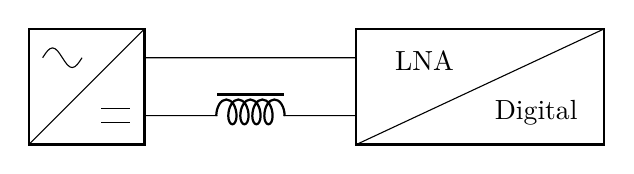
\begin{tikzpicture}[
    big/.style={circuitikz/blocks/scale=1.5},
    long/.style={circuitikz/bipoles/twoportsplit/width=1.5}]
    \path (0,0) node[sacdcshape, big](A){}
        (5,0) node[twoportsplitshape, big, long, t1=LNA, t2=Digital](B){};
    \draw (A.right up) -- (B.left up) (A.right down) to[cute choke] (B.left down);
\end{tikzpicture}
\end{LTXexample}
Notice also from the previous example that the generic blocks (\texttt{twoport} and \texttt{twoportsplit}) can be made ``longer'' by setting different \texttt{width} and \texttt{height} (the other blocks are square, and just use the \texttt{width} key for both dimensions).

Also, for \texttt{amp} and \texttt{vamp}, the \texttt{up} and \texttt{down} anchors follow the shape when they are not boxed.
\begin{LTXexample}[varwidth=true]
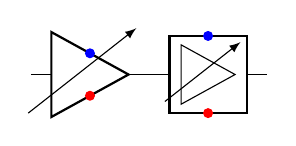
\begin{tikzpicture}
    \draw (0,0) to[vamp, name=a] ++(1.5,0)
        to [vamp, boxed, name=ab] ++(1.5,0);
    \path (a.up) node[circ, blue]{} (ab.up) node[circ, blue]{};
    \path (a.down) node[circ, red]{} (ab.down) node[circ, red]{};
\end{tikzpicture}
\end{LTXexample}

The \texttt{oscillator} has a displaced \texttt{center} anchor, to simplify the task of putting it at the left side of a circuit; it also as a special position for the node text. The four round elements (mixer, circulator, adder, and the oscillator) have a \texttt{geocenter} anchor which always corresponds to the center of the circle.
\begin{LTXexample}[varwidth=true, basicstyle=\small\ttfamily]
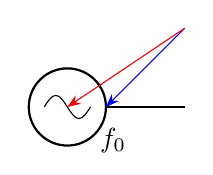
\begin{tikzpicture}[>=Stealth]
    \draw (0,0)node[oscillator](O){$f_0$} -- ++(1,0);
    \draw[blue, ->] (1,1) -- (O.center);
    \draw[red, ->] (1,1) -- (O.geocenter);
\end{tikzpicture}
\end{LTXexample}

Moreover, the have proper border anchors since version \texttt{1.2.3} (and fixed for boxed elements in \texttt{1.5.0}), so you can do things like this:

\begin{LTXexample}[varwidth=true]
\begin{circuitikz}
  \draw (0,0) node[adder] (mix) {}
  (-1,1) -- ++(0.5,0) -- (mix)
  (-1,-1) -- ++(0.5,0) -- (mix) -- ++(1,0);
  \draw [red, <-] (mix.45) -- ++(1,1);
\end{circuitikz}
\end{LTXexample}

Those components have also \textbf{deprecated} anchors named \texttt{1, 2, 3, 4}; they are better not used because they can conflict with the border anchor. They still work for backward compatibility, but could be removed in a future release.

\begin{LTXexample}[varwidth=true]
\begin{circuitikz} \draw
  (0,0) node[mixer] (mix) {}
  (mix.1) node[left] {1} (mix.2) node[below] {2}
  (mix.3) node[right] {3} (mix.4) node[above] {4};
\draw [ultra thick, red, opacity=0.5]
  (-1,-1)--(1,1)(-1,1)--(1,-1);
\node [red, below] at (0,-1) {DON'T USE};
\end{circuitikz}
\end{LTXexample}

The Wilkinson divider has (notice that the node text is outside the bounding box, similarly to what happens for transistors!):

\begin{LTXexample}[varwidth=true]
\begin{circuitikz} \draw
  (0,0) node[wilkinson] (w) {\SI{3}{dB}}
  (w.in) to[short,-o] ++(-0.5,0)
  (w.out1) to[short,-o] ++(0.5,0)
  (w.out2) to[short,-o] ++(0.5,0)
  (w.in) node[below left] {\texttt{in}}
  (w.out1) node[below right] {\texttt{out1}}
  (w.out2) node[above right] {\texttt{out2}}
  ;
\end{circuitikz}
\end{LTXexample}

The couplers have:

\begin{LTXexample}[varwidth=true]
\begin{circuitikz} \draw (0,1.5) %bounding box
  (0,0) node[coupler] (c) {\SI{10}{dB}}
  (c.left down) to[short,-o] ++(-0.5,0)
  (c.right down) to[short,-o] ++(0.5,0)
  (c.right up) to[short,-o] ++(0.5,0)
  (c.left up) to[short,-o] ++(-0.5,0)
  (c.left down) node[below left] {\texttt{left down}}
  (c.right down) node[below right] {\texttt{right down}}
  (c.right up) node[above right] {\texttt{right up}}
  (c.left up) node[above left] {\texttt{left up}}
  ;
\end{circuitikz}
\end{LTXexample}

Or you can also use \texttt{port1} to \texttt{port4} if you prefer:

\begin{LTXexample}[varwidth=true]
\begin{circuitikz} \draw (0,1.5) %bounding box
  (0,0) node[coupler2] (c) {\SI{3}{dB}}
  (c.port1) to[short,-o] ++(-0.5,0)
  (c.port2) to[short,-o] ++(0.5,0)
  (c.port3) to[short,-o] ++(0.5,0)
  (c.port4) to[short,-o] ++(-0.5,0)
  (c.port1) node[below left] {\texttt{port1}}
  (c.port2) node[below right] {\texttt{port2}}
  (c.port3) node[above right] {\texttt{port3}}
  (c.port4) node[above left] {\texttt{port4}}
  ;
\end{circuitikz}
\end{LTXexample}

Also they have the simpler \texttt{1, 2, 3, 4} anchors, and although they have no border anchors (for now), it is better not to use them.

\begin{LTXexample}[varwidth=true]
\begin{circuitikz} \draw(0,1.5) %bounding box
  (0,0) node[coupler] (c) {\SI{10}{dB}}
  (c.1) to[short,-o] ++(-0.5,0)
  (c.2) to[short,-o] ++(0.5,0)
  (c.3) to[short,-o] ++(0.5,0)
  (c.4) to[short,-o] ++(-0.5,0)
  (c.1) node[below left] {\texttt{1}}
  (c.2) node[below right] {\texttt{2}}
  (c.3) node[above right] {\texttt{3}}
  (c.4) node[above left] {\texttt{4}}
  ;
\end{circuitikz}
\end{LTXexample}

\subsubsection{Blocks customization}

You can change the scale of all the block elements by setting the key \texttt{blocks/scale} to something different from the default \texttt{1.0}.

With the option \texttt{>} you can draw an arrow to the input of the block diagram symbols.
\begin{LTXexample}[varwidth=true]
\begin{circuitikz} \draw
  (0,0) to[short,o-] ++(0.3,0)
  to[lowpass,>] ++(2,0)
  to[adc,>] ++(2,0)
  to[short,-o] ++(0.3,0);
\end{circuitikz}
\end{LTXexample}


\paragraph{Multi ports}
Since inputs and outputs can vary, input arrows can be placed as nodes. Note that you have to rotate the arrow on your own:

\begin{LTXexample}[varwidth=true]
\begin{circuitikz} \draw
  (0,0) node[mixer] (m) {}
  (m.w) to[short,-o] ++(-1,0)
  (m.s) to[short,-o] ++(0,-1)
  (m.e) to[short,-o] ++(1,0)
  (m.w) node[inputarrow] {}
  (m.s) node[inputarrow,rotate=90] {};
\end{circuitikz}
\end{LTXexample}


\paragraph{Labels and custom two-port boxes}

You can use the keys \texttt{t}, \texttt{t1}, \texttt{t2} (shorthands for \texttt{text}, \texttt{text in}, \texttt{text out}) to fill the generic blocks:
\begin{LTXexample}[varwidth=true]
\begin{circuitikz} \draw
  (0,0) to[short,o-] ++(0.3,0)
  to[allpass,>] ++(2,0)
  to[twoport,>,t={B}] ++(2,0)
  to[twoportsplit,t1={\tiny in},
    t2={\tiny\color{red}out}] ++(0,-2.5);
\end{circuitikz}
\end{LTXexample}

Some two-ports have the option to place a normal label (\texttt{l=}) and a inner label (\texttt{t=}).
\begin{LTXexample}[varwidth=true]
\begin{circuitikz}
  \ctikzset{bipoles/amp/width=0.9}
  \draw (0,0) to[amp,t=LNA,l_=$F{=}0.9\,$dB,o-o] ++(3,0);
\end{circuitikz}
\end{LTXexample}


\paragraph{Box option}
Several devices have the possibility to add a box around them with the \texttt{box} or \texttt{boxed} option. The inner symbol scales down to fit inside the box. For the ``circled'' devices (mixer, adder, oscillator and circulator) the inner circle is normally drawn, unless you use the \texttt{box only} or \texttt{boxed only} option.\footnote{Since 1.5.0, suggested by \href{https://github.com/circuitikz/circuitikz/issues/621}{GitHub user myzinsky}}
\begin{LTXexample}[varwidth=true]
\begin{circuitikz} \draw
  (0,0) node[mixer, box only, anchor=east](m){}
    to[amp, boxed, >, -o] ++(2.5,0)
  (m.west) node[inputarrow]{} to[short,-o] ++(-0.8,0)
  (m.south) node[inputarrow,rotate=90]{} --
    ++(0,-0.7) node[oscillator, box, anchor=north]{};
\end{circuitikz}
\end{LTXexample}


\paragraph{Dash optional parts}
To show that a device is optional, you can dash it. The inner symbol will be kept with solid lines, unless you set the key \texttt{inner blocks dashed} to true.
Moreover, the key \texttt{dashed blocks pattern} (default \verb|{{1mm}{1mm}}|), be careful with the number of braces!.
\begin{LTXexample}[varwidth=true]
\begin{circuitikz}
\draw (0,1.5) to[amp,l=\SI{10}{dB}] ++(2.5,0);
\draw[dashed] (2.5,1.5) to[lowpass,l=opt.] ++(2.5,0);
% or just the block
\draw (0,0) to[amp,l=\SI{10}{dB}] ++(2.5,0)
     to[lowpass,l=opt., dashed] ++(2.5,0);
% or everything
\ctikzset{inner blocks dashed,
    dashed blocks pattern={{1.5pt}{1pt}},
}
\draw (0,-1.5) to[amp,l=\SI{10}{dB}] ++(2.5,0)
     to[lowpass,l=opt., dashed] ++(2.5,0);
\end{circuitikz}
\end{LTXexample}

\paragraph{Dashing the DC symbol in blocks.}
The symbol for the DC side can be different across countries,\footnote{Head-up from \href{https://github.com/circuitikz/circuitikz/issues/680}{user \texttt{@dbstf} on GitHub}} with different kind of dashing on the bottom line.
Moreover, sometimes the dashing is used to convey different meanings (like rectified sinusoidal or stabilized DC).
You can change the general style for the DC symbol using the key \texttt{blocks dc segments}; using~\texttt{1} (default) will use a continuous line; using \texttt{2} you will have the international-styled symbol, and with~\texttt{3} the English one (you can use higher numbers; the only restriction is that it must be strictly greater than \texttt{0}).  You can also change the input and output part separately with the keys \texttt{blocks dc in segments} and \texttt{blocks dc out segments} (see the following example). The \texttt{inner blocks dashed} option overrides these ones.

\begin{LTXexample}[varwidth=true]
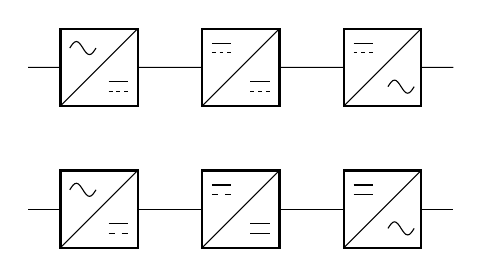
\begin{tikzpicture}[scale=0.9]
    \ctikzset{blocks dc segments=3}
    \draw (0,2) to[sacdc] ++(2,0) to[sdcdc]
        ++(2,0) to[sdcac] ++(2,0);
    \ctikzset{blocks dc segments=1}
    \draw (0,0) to[sacdc, blocks dc out segments=2]
        ++(2,0) to[sdcdc, blocks dc in segments=2]
        ++(2,0) to[sdcac] ++(2,0);
\end{tikzpicture}
\end{LTXexample}

\subsection{Transistors}

\subsubsection{Standard bipolar transistors}

\begin{groupdesc}
    \circuitdesc{npn}{npn}{Q}( B/180/0.2,C/0/0.2,E/0/0.2 )
    \circuitdesc{pnp}{pnp}{}
    \circuitdesc{npn, schottky base}{schottky npn}{}
    \circuitdesc{pnp, schottky base}{schottky pnp}{}
    \circuitdesc{npn, bodydiode}{npn}{}(body C in/60/0.2, body E in/-60/0.2,body C out/0/0.3, body E out/-0/0.3)
    \circuitdesc{npn,photo}{photo npn}{}(nobase/0/0.4)
    \circuitdesc{pnp,photo}{photo pnp}{}(arrows/180/0.1)
    \circuitdesc{nigbt}{nigbt}{Q}
    \circuitdesc{pigbt}{pigbt}{}(centergap/0/0.5)
    \circuitdesc{Lnigbt}{Lnigbt}{Q}
    \circuitdesc{Lpigbt}{Lpigbt}{}
    \circuitdesc{Lpigbt, bodydiode}{Lpigbt}{Q}(body C in/-60/0.2, body E in/60/0.2,body C out/0/0.3, body E out/-0/0.3)
\end{groupdesc}

\subsubsection{Multi-terminal bipolar transistors}

In addition to the standard BJTs transistors, since version~\texttt{0.9.6} the \texttt{bjtnpn} and \texttt{bjtpnp} are also available; these are devices where you can have more collectors and emitters (on the other hand, they have no \texttt{photo} nor \texttt{bodydiode} options --- they are silently ignored).

Basically they are the same as the normal \texttt{npn} and \texttt{pnp}, and they (by default) have similar sizes; the options \texttt{collectors} and \texttt{emitters} will change the number of the relative terminals. The base terminal is connected midway from the collector and the emitter, \emph{not} on the center of the base; a \texttt{cbase} anchor is available if you prefer to use it. The label of the component (the text) is set on the right side, vertically centered around the base terminal. They will accept the \texttt{schottky base} key.

\begin{groupdesc}
    \circuitdesc{bjtnpn, collectors=1, emitters=2}{bjt npn}{Q}(B/180/0.2, C/45/0.2, E/-45/0.2, C1/0/0.4, E1/0/0.4, E2/0/0.4, nobase/135/0.4, cbase/-135/0.4, center/0/0.6)
    \circuitdesc{bjtpnp, collectors=3, emitters=2}{bjt pnp}{Q}(B/180/0.2, C/-45/0.2, E/45/0.2, C1/0/0.4, C2/0/0.4, C3/0/0.4, E1/0/0.4, E2/0/0.4, nobase/135/0.4, cbase/-135/0.4)
\end{groupdesc}

\subsubsection{Field-effect transistors}

\begin{groupdesc}
    \circuitdesc{nmos}{nmos}{Q}( G/180/0.2,D/0/0.2,S/0/0.2 )
    \circuitdesc{pmos}{pmos}{}(centergap/0/0.5)
    \circuitdesc{nmosd}{nmos depletion}{Q}( G/180/0.2,D/0/0.2,S/0/0.2 )
    \circuitdesc{pmosd}{pmos depletion}{}
    \circuitdesc{hemt}{hemt}{}
    \circuitdesc{hemt, nobase}{hemt without base terminal}{Q}( G/180/0.2,D/0/0.2,S/0/0.2, nogate/-120/0.2)
    \circuitdesc{GaN hemt}{Gallium Nitride hemt (a ``styled'' \texttt{hemt}, see~\ref{sec:hemt})}{Q}( G/180/0.2,D/0/0.2,S/0/0.2, nogate/-120/0.2)
\end{groupdesc}

\textsc{nfet}s and \textsc{pfet}s have been incorporated based on code provided by Clemens Helfmeier and Theodor Borsche. Use the package options \texttt{fetsolderdot}/\texttt{nofetsolderdot} to enable/disable solderdot at some fet-transistors. Additionally, the solderdot option can be enabled/disabled for single transistors with the option \texttt{solderdot} and \texttt{nosolderdot}, respectively (You can adjust the size of the solder dot, see section~\ref{sec:solderdot-scale}).

\begin{groupdesc}
    \circuitdesc{nfet}{nfet}{Q}(G/180/0.1, D/0/0.1, S/0/0.1)
    \circuitdesc{nfetd}{nfet depletion}{Q}(G/180/0.1, D/0/0.1, S/0/0.1)
    \circuitdesc{nigfete}{nigfete}{Q}(G/180/0.1, D/0/0.1, S/0/0.1)
    \circuitdesc{nigfete,solderdot}{nigfete}{}(centergap/0/0.5)
    \circuitdesc{nigfetebulk}{nigfetebulk}{}
    \circuitdesc{nigfetd}{nigfetd}{}(centergap/0/0.5)
    \circuitdesc{pfet}{pfet}{Q}(G/180/0.1, D/0/0.1, S/0/0.1)
    \circuitdesc{pfetd}{pfet depletion}{Q}(G/180/0.1, D/0/0.1, S/0/0.1)
    \circuitdesc{pigfete}{pigfete}{}(centergap/0/0.5, G/180/0.1, D/0/0.1, S/0/0.1)
    \circuitdesc{pigfetebulk}{pigfetebulk}{}
    \circuitdesc{pigfetd}{pigfetd}{}
\end{groupdesc}

Since version \texttt{1.6.0}, you can add the \texttt{doublegate} option to the \texttt{*igfet*} family of devices to have a double gate MOS --- the additional gate is called \texttt{G2} or \texttt{gate2} (the plain \texttt{G} is where it will be without the \texttt{doublegate} option).

\begin{groupdesc}
    \circuitdesc{nigfete, doublegate}{nigfete, doublegate}{Q}(G/180/0.1, G2/180/0.1, D/0/0.1, S/0/0.1)
    \circuitdesc{nigfete,solderdot, doublegate}{nigfete, doublegate}{}(G1/180/0.1, centergap/0/0.5, G2/180/0.1)
    \circuitdesc{nigfetebulk, doublegate}{nigfetebulk, doublegate}{}(G/180/0.1, G2/180/0.1)
    \circuitdesc{nigfetd, doublegate}{nigfetd, doublegate}{}(G1/180/0.1, centergap/0/0.5, G2/180/0.1)
    \circuitdesc{pigfete, doublegate}{pigfete, doublegate}{}(G/180/0.1, centergap/0/0.5, G2/180/0.1, D/0/0.1, S/0/0.1)
    \circuitdesc{pigfetebulk, doublegate}{pigfetebulk, doublegate}{}(G/180/0.1, G2/180/0.1)
    \circuitdesc{pigfetd, doublegate}{pigfetd, doublegate}{}(G1/180/0.1, G2/180/0.1)
\end{groupdesc}

You can use the double-gated transistor for example like this:%
\footnote{Found at \href{https://www.electronics-notes.com/articles/electronic_components/fet-field-effect-transistor/dual-gate-mosfet.php}{this page on electronics notes}.}

\begin{LTXexample}[varwidth=true, basicstyle=\scriptsize\ttfamily]
\begin{circuitikz}[european, scale=0.7, transform shape,
    circuitikz/resistors/scale=0.7]
    \draw (0,0) to[C, o-*] ++(1,0) coordinate(in)
    to[R, -*] ++(0,-3) coordinate(GND)
    ++(1,0) to[C, *-] ++(0,4) -- ++(1,0) coordinate(div)
    to[R, *-*] ++(0,2) coordinate(vdd)
    (div) to[R, -*] (div|-GND)
    (in) -- ++(2.5,0) node[nigfetd, doublegate, anchor=G1](Q){Q}
    (Q.G2) to[short, -*] (Q.G2-|div)
    (Q.D) to[R, -*] (Q.D|-vdd)
    (Q.D) to[C, *-o] ++(2,0) coordinate(out)
    (Q.S) to[R, *-*] (Q.S|-GND) (Q.S) -- ++(1,0) coordinate(Sd)
    (Sd) to[C, -*] (Sd |- GND);
    \draw (0,0|-GND) -- (out|-GND) (0,0|-vdd) -- (out|-vdd);
\end{circuitikz}
\end{LTXexample}

\textsc{JFET} are also available\footnote{based on code provided by Danilo Piazzalunga}, both n-type and p-type.

\begin{groupdesc}
    \circuitdesc{njfet}{n-type JFET}{Q}(G/-135/0.2,D/0/0.2,S/0/0.2)
    \circuitdesc{pjfet}{p-type JFET}{}(G/-135/0.2,D/0/0.2,S/0/0.2)
\end{groupdesc}

\textsc{UJT} transistors\footnote{sugged by \href{https://github.com/circuitikz/circuitikz/issues/522}{user JetherReis on GitHub}.} have a different anchor names although \textbf{most} of the others, like \texttt{D} and \texttt{G}, also work (the exception is \texttt{E} and \texttt{emitter}!). Notice that if used with \texttt{nobase}, the anchor \texttt{E} follows the wire, while \texttt{G} is fixed (as is \texttt{kink}).

\begin{groupdesc}
    \circuitdesc{nujt}{n-type UJT}{Q}(G/-135/0.2,B1/0/0.2,B2/0/0.2 , kink/90/0.4, E/135/0.2)
    \circuitdesc{pujt}{p-type UJT}{Q}(G/-135/0.2,B1/0/0.2,B2/0/0.2 , kink/90/0.4, E/135/0.2)
    \circuitdesc{nujt, nobase}{n-type UJT with nobase option}{Q}(G/-135/0.2,B1/0/0.2,B2/0/0.2 , kink/90/0.4, E/135/0.2)
\end{groupdesc}

\textsc{isfet}:

\begin{groupdesc}
    \circuitdesc{isfet}{isfet}{Q}
\end{groupdesc}

\textsc{Graphene fet} have been added in version \texttt{1.3.2}\footnote{added by Romano Giannetti after a suggestion by Cees Keyer.}. They look better if you set \texttt{transistors/arrow pos=end} and \texttt{transistor/thickness=3} or higher for them, so they are plotted with this option here.
\begin{groupdesc}
    \ctikzset{transistors/thickness=3, transistors/arrow pos=end}
    \circuitdesc*{ngfet}{N-type graphene FET}{Q}(outer hex up/45/0.3, outer hex down/-45/0.3, right/0/0.4)
    \circuitdesc*{pgfet}{pgfet}{Q}(inner hex up/135/0.3, inner hex down/-135/0.3)
\end{groupdesc}

\subsubsection{Transistor texts (labels)}\label{sec:transistors-labels}

In versions before \texttt{0.9.7}, transistors text (the node text) was positioned near the collector terminal; since version \texttt{0.9.7} the default has been changed to a more natural position near the center of the device, similar to the multi-terminal transistors. You can revert to the old behavior locally with the key \texttt{legacy transistors text}, or globally by setting the package option \texttt{legacytransistorstext}.

Notice the use of the utility functions \verb|\ctikzflip{|\texttt{\textsl{x,y,xy}}\verb|}| as explained in section~\ref{sec:mirroring-and-flipping}.

\begin{LTXexample}[varwidth=true]
\begin{circuitikz}[scale=0.8, transform shape]
    \draw (0,0) node [npn]{T1}
    ++(1.2,0) node [npn, xscale=-1]{\ctikzflipx{T1}}
    ++(2,0) node [npn, yscale=-1]{\ctikzflipy{T1}}
    ++(1.2,0) node [npn, scale=-1]{\ctikzflipxy{T1}};
    \ctikzset{legacy transistors text}
    \draw (0,-2) node [npn]{T1}
    ++(1.2,0) node [npn, xscale=-1]{\ctikzflipx{T1}}
    ++(2,0) node [npn, yscale=-1]{\ctikzflipy{T1}}
    ++(1.2,0) node [npn, scale=-1]{\ctikzflipxy{T1}};
\end{circuitikz}
\end{LTXexample}

\subsubsection{Transistors customization}\label{sec:styling-transistors}

\paragraph{Size.} You can change the scale of all the transistors by setting the key \texttt{transistors/scale} (default \texttt{1.0}).
The size of the arrows (if any) is controlled by the same parameters as \texttt{currarrow} (see section~\ref{sec:currarrow-size}) and the dots on P-type transistors (if any) are the same as the nodes/poles (see section~\ref{sec:bipole-nodes}).

\paragraph{Arrows.} The default position of the arrows in transistors is somewhat in the middle of the terminal; if you prefer you can move them to the end with the style key \texttt{transistors/arrow pos=end} (the default value is \texttt{legacy}).

\begin{LTXexample}[varwidth=true]
\begin{circuitikz}
   \ctikzset{tripoles/mos style=arrows}
   \ctikzset{transistors/arrow pos=end}
   \draw (0,0) node[npn, ](npn){};
   \draw (2,0) node[pnp, ](npn){};
   \draw (0,-2) node[nmos, ](npn){};
   \draw (2,-2) node[pmos, ](npn){};
\end{circuitikz}
\end{LTXexample}

If the option \texttt{arrowmos} is used (or after the command \verb!\ctikzset{tripoles/mos style/arrows}! is given), this is the output:
\begin{groupdesc}
        \ctikzset{tripoles/mos style/arrows}
	\circuitdesc{nmos}{nmos}{}
	\circuitdesc{pmos}{pmos}{}
    \circuitdesc{nmosd}{nmos depletion}{}
    \circuitdesc{pmosd}{pmos depletion}{}
\end{groupdesc}

You can go back to the no-arrows mos with \texttt{noarrowmos} locally or with
\texttt{\textbackslash ctikzset\{tripoles/mos style/no arrows\}}.

To draw the PMOS circle non-solid, use the option \texttt{emptycircle} or the command
\\\verb!\ctikzset{tripoles/pmos style/emptycircle}!. To remove the dot completely (only useful if you have \texttt{arrowmos} enabled, otherwise there will be no difference between P-MOS and N-MOS), you can use the option \texttt{nocircle} or \verb|\ctikzset{tripoles/pmos style/nocircle}|.

\begin{groupdesc}
    \circuitdesc{pmos,emptycircle}{pmos}{}
    \circuitdesc{pmos,nocircle,arrowmos}{pmos}{}
\end{groupdesc}

This example show the combined effects of the arrows and gate-circle options:

\begin{LTXexample}[varwidth=true]
\begin{circuitikz}[
    info/.style={left=1cm, blue, text width=5em, align=right},]
    \draw (0,1) node{pmos} (2,1) node{nmos};
    \draw (0,0) node[info]{default} node[pmos]{} (2,0) node[nmos]{};
    \ctikzset{tripoles/mos style/arrows}
    \draw (0,-2) node[info]{arrows} node[pmos]{} (2,-2) node[nmos]{};
    \ctikzset{tripoles/pmos style/emptycircle}
    \draw (0,-4) node[info]{emptycircle} node[pmos]{} (2,-4) node[nmos]{};
    \ctikzset{tripoles/pmos style/nocircle}
    \draw (0,-6) node[info]{nocircle} node[pmos]{} (2,-6) node[nmos]{};
    \ctikzset{tripoles/mos style/no arrows}
    \draw (0,-8) node[info, red]{no circle, no arrows, DON'T do it}
          node[pmos]{} (2,-8) node[nmos]{};
\end{circuitikz}
\end{LTXexample}

You can also change\footnote{Thanks to the idea by \href{https://github.com/circuitikz/circuitikz/issues/655}{Dr. Matthias Jung on GitHub}.} the type of the arrow for the ``light rays'' of the phototransistors with the generic arrows options shown in~\ref{sec:tunablearrows}, using the name \texttt{opto}, like in the following (overdone) example. Also the \texttt{opto arrows} styling options (see section~\ref{sec:opto-arrows}).

\begin{LTXexample}[varwidth=true, basicstyle=\small\ttfamily]
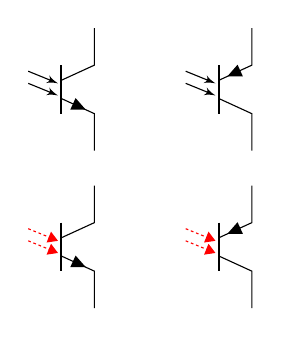
\begin{tikzpicture}
    \draw (0,2) node[npn, photo]{} ++(2,0) node[pnp, photo]{};
    \ctikzset{opto end arrow={Triangle[angle'=60]}}
    \ctikzset{opto arrows/.cd, color=red, dash={{1pt}{1pt}}}
    \draw (0,0) node[npn, photo]{} ++(2,0) node[pnp, photo]{};
\end{tikzpicture}
\end{LTXexample}

\paragraph{Circles.} Since \texttt{1.2.6}, you can add a circle\footnote{Suggested by Matthias Jung \href{https://github.com/circuitikz/circuitikz/issues/442}{on GitHub}} to most of the transistor shapes --- with the exception of multi-terminal (\texttt{bjtnpn} and \texttt{bjtpnp}, where it would be awkward anyway) and graphene FETs. The circle is intended in some case as the component's housing, and used to distinguish discrete components from integrated ones.

To add the circle to a single transistor, you use the \texttt{tr circle} keys in the node; if you want all of your transistors with a circle, you can set the property \texttt{tr circle} with a \verb|\ctikzset| command (it will respect normal grouping, of course); in that case, you can use \texttt{tr circle=false} to locally disable them.

\begin{LTXexample}[varwidth=true]
\begin{circuitikz}[]
    \draw (0,2) node[npn]{} (2,2) node[npn, tr circle](Q){};
    % collector connected to housing
    \node [circ] at (Q.circle C){};
    \ctikzset{tr circle=true} % or \ctikzset{tr circle} alone
    \draw (0,0) node[nigfete]{}
        (2,0) node[nigfete, tr circle=false]{};
\end{circuitikz}
\end{LTXexample}

You can tweak the appearance of transistor's circles and even draw it partially; see ~\ref{sec:trans-circle-custom} for details.

\paragraph{Body diodes and similar things.}\label{sec:bodydiodes-anchor} For all transistors (minus \texttt{bjtnpn} and \texttt{bjtpnp})  a body diode (or freewheeling or flyback diode) can automatically be drawn. Just use the global option \texttt{bodydiode}, or for single transistors, the \TikZ-option \texttt{bodydiode}.
As you can see in the next example, the text for the diode is moved if a bodydiode is present (but beware, if you change a lot the relative dimension of components, it may become misplaced):

\begin{LTXexample}[varwidth=true]
\begin{circuitikz}
   \draw (0,0) node[npn,bodydiode](npn){1}
       ++(2,0)node[pnp,bodydiode](npn){};
   \draw (0,-2) node[nigbt,bodydiode](npn){2}
       ++(2,0)node[pigbt,bodydiode](npn){};
   \draw (0,-4) node[nfet,bodydiode](npn){3}
       ++(2,0)node[pfet,bodydiode](npn){};
\end{circuitikz}
\end{LTXexample}

You can tweak the appearance of transistor's bodydiodes; see ~\ref{sec:trans-bodydiode-custom}.

For more complex snubs or protections, you can use the \texttt{body ...} anchors to add more or different things to the transistors in addition (or instead) of the flyback diode.

\begin{LTXexample}[varwidth=true]
\def\snubb#1#2{% add a snubber to a transistor
    \draw (#1.body C #2) to[short, *-, nodes width=0.02]
    ++(0.3,0) coordinate(tmp) to [R, resistors/scale=0.3]
    % 2/3 space for R, 1/3 for C
    ($(tmp)!0.66!(tmp|-#1.body E #2)$)
    to [C, capacitors/scale=0.3] (tmp|-#1.body E #2)
    to [short, -*, nodes width=0.02] (#1.body E #2);
}
\begin{circuitikz}
    \node[npn](Q1) at(0,0) {};
    \node[pnp](Q2) at(2,0) {};
    \node[pnp, bodydiode](Q3) at(0,-3) {};
    \node[npn, bodydiode](Q4) at(2,-3) {};
    \snubb{Q1}{in} \snubb{Q2}{in}
    \snubb{Q3}{out} \snubb{Q4}{out}
\end{circuitikz}
\end{LTXexample}

\paragraph{HEMT customization.\label{sec:hemt}} Since \texttt{v1.6.1} the shape of the \texttt{hemt} transistor can be customized.\footnote{After a suggestion from \href{https://github.com/circuitikz/circuitikz/issues/691}{user \texttt{@epsilon-phi} on GitHub}.}
There are several keys under the hierarchy \texttt{tripoles/hemt} that can be use to change the appearance; some of them are common to other transistors and some are specific.

The main ones are \texttt{\dots/split gate} (boolean, default \texttt{false}) that will create a ``split'' gate, which sometimes is used to convey that the device is enhancement-type;
\texttt{source arrow} (default \texttt{0}), to add an arrow on the source terminal (\texttt{1} for a right-facing one, \texttt{-1} the other way around; the arrow will obey \texttt{arrow pos=end} if issued, but otherwise the position is fixed);
\texttt{gate asym} (default \texttt{0.0}) which displaces the gate asymmetrically. For example, the \texttt{GaN hemt} component is really a styled \texttt{hemt} (predefined), with the definition:

\begin{lstlisting}
\tikzset{GaN hemt/.style={hemt,
        circuitikz/tripoles/hemt/base height=0.6,% length of the "base" vertical bar
        circuitikz/tripoles/hemt/gate height=0.5,% distance of the S/D terminals
        circuitikz/tripoles/hemt/bodydiode conn=0.85,% attachment point of body diode
        circuitikz/tripoles/hemt/gate asym=-0.1,% slightly down
        circuitikz/tripoles/hemt/split gate=true,% split gate
        circuitikz/tripoles/hemt/source arrow=1,% right-facing arrow
    },
}
\end{lstlisting}

\begin{LTXexample}[varwidth=true]
\begin{circuitikz}[]
    \path (-1,-1) rectangle (3,3);% bounding box
    \node  [hemt] at (0,2) {A};
    \node  [hemt,
        circuitikz/tripoles/hemt/split gate=true
        ] at (2,2) {B};
    \node  [GaN hemt]  at (0,0) {C};
    \node  [GaN hemt,
        circuitikz/tripoles/hemt/split gate=false
        ]  at (2,0) {D};
\end{circuitikz}
\end{LTXexample}

\paragraph{Schottky transistors.}
The Schottky transistors are generated by adding the \texttt{schottky base} key (there is also a \texttt{no schottky base} key that can be used if you use the other one as a default).
You can change the size of the Schottky ``hook'' changing the parameter \texttt{tripoles/schottky base size} with \verb|\ctikzset{}| (default \texttt{\ctikzvalof{tripoles/schottky base size}}; the unit is the standard resistor length, scaled if needed.)

\begin{LTXexample}[varwidth=true]
    \begin{circuitikz}
        \draw (0,4) node[npn]{}
            ++(2,0) node[npn, schottky base]{};
        \draw (1,2) node[bjtnpn, collectors=2, emitters=3,
            schottky base, rotate=90]{};
        \tikzset{schottky base}
        \ctikzset{tripoles/schottky base size=0.1}
        \draw (0,0) node[pnp]{}
            ++(2,0) node[npn, no schottky base]{};
    \end{circuitikz}
\end{LTXexample}

\paragraph{Ferroelectric transistors} You can add the ferroelectric modifier\footnote{suggested by \href{https://github.com/circuitikz/circuitikz/issues/515}{Mayeul Cantan}} to the \texttt{*mos} and \texttt{*fet} transistor  types. Similarly to the Schottky bipolar transistors, you activate it by adding the \texttt{ferroel gate} key (there is also a \texttt{no ferroel base} key that can be used if you use the other one as a default).

The mark will follow the \texttt{transistors} class thickness, but you can adjust it independently using the class parameter \texttt{modifier thickness} as in passive components --- this value is relative to the class' thickness.

\begin{LTXexample}[varwidth=true]
    \begin{circuitikz}
        \draw (0,2) node[nmos]{}
            ++(2,0) node[nmos, ferroel gate]{};
        \ctikzset{ferroel gate} % by default from now on
        \ctikzset{transistors/.cd, % class properties
            thickness=1, modifier thickness=3}
        \draw (0,0) node[pfet]{}
            ++(2,0) node[pfet, no ferroel gate]{};
    \end{circuitikz}
\end{LTXexample}


\paragraph{IGBT outer base.}
Normally, in bipolar IGBTs the outer base is the same size (height) of the inner one, and of the same thickness (which will depend on the class thickness value). You can change this by setting (via \verb|\ctikzset|) the keys \texttt{tripoles/igbt/outer base height} (default \texttt{0.4}, the same as \texttt{base height}), and \texttt{tripoles/igbt/outer base thickness} (default \texttt{1.0}), which will be relative to the class thickness.

\begin{LTXexample}[varwidth=true, pos=t]
\begin{circuitikz}
    \draw (0,0)
    -- ++(1,0) node[nigbt, anchor=B](B){} (B.nobase)
    -- ++(1,0) node[pigbt, anchor=B](B){} (B.nobase)
    -- ++(1,0) node[Lnigbt, anchor=B](B){} (B.nobase)
    -- ++(1,0) node[Lpigbt, anchor=B](B){} (B.nobase)
    ;
    \ctikzset{tripoles/igbt/outer base height=0.3}
    \ctikzset{tripoles/igbt/outer base thickness=1.5}
    \draw (6,0)
    -- ++(1,0) node[nigbt, anchor=B](B){} (B.nobase)
    -- ++(1,0) node[pigbt, anchor=B](B){} (B.nobase)
    -- ++(1,0) node[Lnigbt, anchor=B](B){} (B.nobase)
    -- ++(1,0) node[Lpigbt, anchor=B](B){} (B.nobase)
    ;
\end{circuitikz}
\end{LTXexample}

\paragraph{UJT transistors.}\label{sec:ujt} They look better if you use \texttt{transistors/arrow pos=end}, especially if you use them with \texttt{tr circle}. If you use the key \texttt{nobase} with UJTs, the horizontal part of the controlling terminal is not drawn; notice that this \emph{will} move the \texttt{E} or \texttt{emitter} anchor, but not the generic ones like \texttt{G}.

\begin{LTXexample}[varwidth=true, basicstyle=\footnotesize\ttfamily]
\begin{circuitikz}[scale=0.8]
    \draw (0,5) node[nujt]{} ++(2,0) node[pujt]{}
    ++(2,0) node[nujt, tr circle]{} ++(2,0)
    node[pujt, tr circle]{};
    \ctikzset{transistors/arrow pos=end}
    \draw (0,2.5) node[nujt](A){} ++(2,0) node[pujt]{}
    ++(2,0) node[nujt, tr circle]{} ++(2,0)
    node[pujt, tr circle](C){};
    \draw (0,0) node[nujt, nobase](B){} ++(2,0)
    node[pujt, nobase]{} ++(2,0)
    node[nujt, tr circle, nobase]{} ++(2,0)
    node[pujt, tr circle, nobase](D){};
    % "E" anchor follows the nobase option:
    \draw[red] (A.E) |- (B.E) (C.E) |- (D.E);
\end{circuitikz}
\end{LTXexample}

\paragraph{Base/Gate terminal.} The Base/Gate connection of all transistors can be disabled by the options \textit{nogate} or \textit{nobase}, respectively. The Base/Gate anchors are floating, but there is an additional anchor \texttt{nogate}/\texttt{nobase} , which can be used to point to the unconnected base:
\begin{LTXexample}[varwidth=true]
\begin{circuitikz}
   \draw (2,0) node[npn,nobase](npn){};
   \draw (npn.E) node[below]{E};
   \draw (npn.C) node[above]{C};
   \draw (npn.B) node[circ]{} node[left]{B};
   \draw[dashed,red,-latex] (1,0.5)--(npn.nobase);
\end{circuitikz}
\end{LTXexample}

\paragraph{Bulk terminals.} You can add a bulk terminal\footnote{Thanks to Burak Kelleci <kellecib@hotmail.com>.} to \texttt{nmos} and \texttt{pmos} using the key \texttt{bulk} in the node (and \texttt{nobulk} if you set the bulk terminal by default); additional anchors \texttt{bulk} and \texttt{nobulk} are added (in the next example, \texttt{tripoles/mos style/arrows} is enacted, too):

\begin{groupdesc}
    \ctikzset{tripoles/mos style/arrows}
    \circuitdesc{nmos, bulk}{pmos}{}(bulk/45/0.3, nobulk/-30/.4)
    \circuitdesc{pmos, bulk}{pmos}{}
    \circuitdesc{nmosd, bulk}{nmos depletion}{}(bulk/45/0.3, nobulk/-30/.4)
    \circuitdesc{pmosd, bulk}{pmos depletion}{}
    \circuitdesc{nigbt}{nigbt}{}(nobase/135/0.3, nobulk/-30/.4)
    \circuitdesc{pigbt, nobase}{pigbt with no base terminal\footnotemark}{}(nobase/135/0.3, nobulk/-30/.4)
    \footnotetext{Since \texttt{v1.4.4}, noticed by \href{https://tex.stackexchange.com/q/619334/38080}{user \texttt{hinata exc} on Stack Exchange}.}
\end{groupdesc}


\paragraph{Solder dots.}\label{sec:solderdot-scale}
Solder dots are scaled-down\footnote{Since \texttt{v1.6.3}, suggested by \href{https://tex.stackexchange.com/q/687225/38080}{user Hartomes on TeX StackExchange}; previously, the default scale was \texttt{1.0}, which created a clash with body diodes.} version of the normal \texttt{circ} connection dot (\emph{pole}).
This is to convey the information that the connection is \emph{internal} to the device, and not controllable from the outside. By default, they are scaled as the bodydiode connection dots (see section~\ref{sec:trans-bodydiode-custom}), but you can change them with the command \texttt{\textbackslash ctikzset\{transistor solderdot scale=\emph{x}\}}, where $x$ is the scale with respect to the normal \texttt{circ} node (default: \texttt{0.7}).

\begin{LTXexample}[varwidth=true]
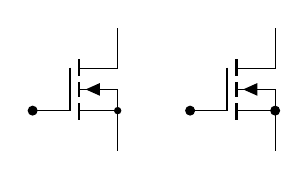
\begin{tikzpicture}[]
    \draw (0,0) to[short,*-] ++(.1,0)
        node[nigfete, solderdot, anchor=G]{};
    \ctikzset{transistor solderdot scale=1}
    \draw (2,0) to[short,*-] ++(.1,0)
        node[nigfete, solderdot, anchor=G]{};
\end{tikzpicture}
\end{LTXexample}

\paragraph{Simplified symbols for depletion-mode MOSFETs}.
The \texttt{nmosd}, \texttt{pmosd} (symplified) symbols for depletion-mode MOSFET (introduced in \texttt{1.2.4}) behave exactly like the normal (without the final \texttt{d}) ones.

By default, the thick bar (indicating the pre-formed channel) is filled with the same color as the drawing:
\begin{LTXexample}[varwidth=true]
\begin{circuitikz}[ ]
    \draw (0,2) to[R] ++(2,0) node[nmosd, anchor=G]{};
    \draw[color=red] (0,0) to[R] ++(2,0) node[pmosd, anchor=G]{};
\end{circuitikz}
\end{LTXexample}

You can change this behavior by setting the key
\texttt{tripoles/nmosd/depletion color} (default value \texttt{default}, which means ``use the draw color'') to the color you want; using \texttt{none} will lead to an unfilled channel (note that in this case the color does not change automatically with the path!):
\begin{LTXexample}[varwidth=true]
\begin{circuitikz}[ ]
    \ctikzset{tripoles/nmosd/depletion color=gray}
    \draw (0,2) to[R] ++(2,0) node[nmosd, anchor=G]{};
    \ctikzset{tripoles/pmosd/depletion color=none}
    \draw[color=red] (0,0) to[R] ++(2,0)
        node[pmosd, anchor=G]{};
    \ctikzset{tripoles/pmosd/depletion color=
        {cyan!50!white}}
    \draw[color=blue] (0,-2) to[R] ++(2,0)
        node[pmosd, anchor=G, bulk]{};
\end{circuitikz}
\end{LTXexample}


Obviously you have the equivalent \texttt{tripoles/pmosd/depletion color} for type-P transistors.

They also have path-style syntax, as the other transistors.

\begin{LTXexample}[varwidth=true]
\begin{circuitikz}[ ]
    \draw (0,0) to[Tnmosd] ++(2,0)
    to[Tpmosd, invert] ++(0,-2)
    ;
\end{circuitikz}
\end{LTXexample}

\paragraph{Gate/Base gap coloring.} You can color the space representing the gate capacitor or the insulated base by using the key \texttt{tr gap fill} (default \texttt{none}, which means nothing is drawn there). This fill is done \emph{after} any circle fill but before any additional modifier (see the example below). You can use it locally or set it globally (normal scoping works, as ever).

\begin{LTXexample}[varwidth=true]
    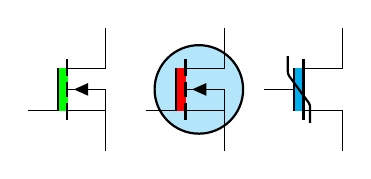
\begin{tikzpicture}
        \node[nigfete, tr gap fill=green] at(0,0){};
        \node[nigfete, tr gap fill=red, tr circle,
            fill=cyan!30] at(1.5,0){};
        \node[nmos, tr gap fill=cyan, ferroel gate](A)
            at(3,0){};
    \end{tikzpicture}
\end{LTXexample}

\subsubsection{Multiple terminal transistors customization}

You can create completely ``bare'' transistors (without the connection leads to the \texttt{B}, \texttt{C} y \texttt{E} terminals), by changing the parameter \texttt{tripoles/bjt/pins width} (default \texttt{0.3}; it is expressed as a fraction of the basic (scaled) length) or using the style \texttt{bjt pins width}; and you can change the distance between multiple collectors/emitters setting with \verb|\ctikzset{}|  the parameter \texttt{tripoles/bjt/multi height}  (default \texttt{0.5}) or the style \texttt{bjt multi height}.

\begin{groupdesc}
    \circuitdesc{bjtnpn, collectors=2, emitters=2, bjt pins width=0, bjt multi height=0.8}{bjt npn with parameters}{Q}(B/180/0.2, C/45/0.2, E/-45/0.2, C1/0/0.4, C2/0/0.4, E1/0/0.4, E2/0/0.4, nobase/-135/0.4, cbase/135/0.4)
\end{groupdesc}


\subsubsection{Transistor circle customization}\label{sec:trans-circle-custom}

\paragraph{Position and size.} You can see in the following diagram where the circle is positioned --- when there is no bodydiode, it will pass through the anchors for the body diode and near the base connection. The dimension of the circle is bigger when the bodydiode is in, to encompass it.
The anchors are present even if there is no circle, so you can use them to draw different kinds of circles (say, encompassing two transistors) in a coherent way.

\circuitdesc{npn, tr circle}{npn with a circle}{}(circle base/90/0.5, circle C/30/0.2, circle E/-30/0.2, circle center/0/0.5)
\circuitdesc{npn, tr circle, bodydiode}{npn with a circle}{}(circle base/90/0.6, circle C/30/0.2, circle E/-30/0.2, circle center/0/0.5 )

The position of the circle on collector and emitter by default is the one shown above; the position along the base can be adjusted in most transistors using the \verb|\ctikzset| parameter \texttt{transistor circle/default base in} (by default \texttt{\ctikzvalof{transistor circle/default base in}}); \texttt{njfet} and \texttt{pjfet} use \texttt{transistor circle/njfet base in} (default \texttt{\ctikzvalof{transistor circle/njfet base in}}; the same for \texttt{pjfet}) and, finally, \texttt{isfet} uses \texttt{transistor circle/isfet base in} (default \texttt{\ctikzvalof{transistor circle/isfet base in}}). You can change the resulting size of the circle by setting to something different to \texttt{1.0} the parameter \texttt{transistor circle/scale circle radius} --- that will move the anchors too; for example:

\begin{LTXexample}[varwidth=true]
\begin{circuitikz}[scale=1.5, transform shape]
    \draw (0,0) node[npn, tr circle](Q1){};
    \node [circ] at (Q1.circle C){};
    \ctikzset{transistor circle/scale circle radius=1.2}
    \draw[color=red] (0,0) node[npn, tr circle](Q2){};
    \node [circ, color=red] at (Q2.circle C){};
\end{circuitikz}
\end{LTXexample}

\paragraph{Line and color.} Normally the circle follows the style of the component --- the line thickness is fixed by the class element \texttt{transistors/thickness} and the color is the same as the component color. You can change, if you need, all of these things using the parameters of the following table (the parameters are under the \verb|\ctikzset| category root \texttt{transistor circle/}.

\begin{center}
    \begin{tabular}{>{\ttfamily}l>{\ttfamily}ll}
        \toprule
     parameter &  default & description  \\
     \midrule
     relative thickness & 1.0 & multiply the class thickness \\
     color & default & stroke color: \texttt{default} is the same as the component \\
     dash & default & dash pattern: none means solid line, default means keep the global pattern\footnotemark \\
     partial borders & none & draw only part of the circle border: none means draw all \\
     partial border dash & \{\{2pt\}\{2pt\}\} & dash pattern used in partial borders \\
        \bottomrule
    \end{tabular}
    \footnotetext{Follows the syntax of the pattern sequence \texttt{\textbackslash pgfsetdash} --- see \TikZ{} manual for details; phase is always zero. Basically you pass pairs of dash-length -- blank-length dimensions, see the examples.}
\end{center}

\begin{LTXexample}[varwidth=true]
\begin{circuitikz}[]
    \draw (0,2) node[npn, tr circle](Q1){};
    \ctikzset{transistor circle/relative thickness=2}
    \draw (2,2) node[npn, tr circle](Q1){};
    \ctikzset{transistor circle/color=red}
    \draw (0,0) node[npn, tr circle](Q1){};
    \ctikzset{transistor circle/color=default}
    \ctikzset{transistor circle/dash={{4pt}{4pt}{1pt}{4pt}}}
    \draw[color=blue] (2,0) node[npn, tr circle](Q1){};
\end{circuitikz}
\end{LTXexample}

Finally, using the class style you can do quite interesting things.

\begin{LTXexample}[varwidth=true]
\begin{circuitikz}[]
    \ctikzset{transistors/thickness=4, transistors/fill=cyan!30,
        transistor circle/relative thickness=0.25,}
    \draw (0,0) node[npn, tr circle](Q1){};
    \ctikzset{transistor circle/dash={{2pt}{2pt}}}
    \draw (1.5,0) node[npn, tr circle, xscale=-1](Q2){};
\end{circuitikz}
\end{LTXexample}

\paragraph{Partially drawn circle borders}

In some circuits, transistors are drawn with partial or dashed border (to convey the meaning of several active components encased in the same physical package, or to signify thermal contact). To achieve this effect, you can use the \texttt{transistor circle/partial border}\footnote{Suggested by \href{https://github.com/circuitikz/circuitikz/issues/602}{Jether Fernandes Reis} for tubes, implemented by Romano in \texttt{v1.5.2}.} key (default \texttt{none}). This key can be set to \texttt{none}, or must be a sequence of \textbf{exactly} 4 numbers, that can have value \texttt{0}, \texttt{1}, or \texttt{2}. Each number defines the style of a part of the border to be not drawn, solid or dashed respectively.

The part of the border are numbered from 1 to 4 as shown below:
\begin{quote}
\begin{circuitikz}[circuitikz/transistors/fill=cyan!20,
            circuitikz/transistor circle/partial borders=1212]
            \draw (0,0) node[npn, tr circle](T){};
            \draw[red, font=\ttfamily\small\bfseries]
                ([shift={(.3,-.2)}]T.north east) node{1}
                ([shift={(.3,.2)}]T.south east) node{2}
                ([shift={(.2,.2)}]T.south west) node{3}
                ([shift={(.2,-.2)}]T.north west) node{4}
                ;
    \end{circuitikz}
\end{quote}
The dashed line pattern can be changed by setting the key \texttt{transistor circle/partial border dash} (default \verb|{{2pt}{2pt}}|). Be careful with the extra set of braces here.

\begin{LTXexample}[varwidth=true]
\begin{circuitikz}[]
    \ctikzset{transistors/thickness=4, transistors/fill=cyan!30,
        transistor circle/relative thickness=0.25,
        transistor circle/partial borders=2211}
    \draw (0,0) node[npn, tr circle](Q1){};
    \ctikzset{transistor circle/dash={{2pt}{2pt}}}
    \draw (1.5,0) node[npn, tr circle, xscale=-1](Q2){};
\end{circuitikz}
\end{LTXexample}

\begin{LTXexample}[varwidth=true]
\begin{circuitikz}[]
    \ctikzset{transistors/thickness=4, transistors/fill=cyan!30,
        transistor circle/relative thickness=0.25,
        transistor circle/partial borders=0011}
    \draw (0,0) node[npn, tr circle](Q1){};
    \ctikzset{transistor circle/dash={{2pt}{2pt}}}
    \draw (1.5,0) node[npn, tr circle, xscale=-1](Q2){};
    \draw[dashed] (Q1.circle top) -- (Q2.circle top);
    \draw[dashed] (Q1.circle bottom) -- (Q2.circle bottom);
\end{circuitikz}
\end{LTXexample}

\subsubsection{Transistor bodydiode customization}\label{sec:trans-bodydiode-custom}

You can change the style of the bodydiode\footnote{Suggested by \href{https://tex.stackexchange.com/questions/653348/drawing-mosfet-bodydiode-dashed}{user Alex Ghilas on TeX.SX}, implemented in \texttt{v1.5.4}; \texttt{scale} suggested by \href{https://github.com/circuitikz/circuitikz/issues/703}{user \texttt{@sputeanus} on GitHub} and added in version \texttt{1.6.2}.} in a similar way to the one used for circles (albeit with less options), by setting keys with the \verb!\ctikzset! command (or, like in the following example, directly in the node instantiation) under the \texttt{transistor bodydiode} hierarchy. The available keys are:

\begin{center}
    \begin{tabular}{>{\ttfamily}l>{\ttfamily}lp{0.5\linewidth}}
        \toprule
     parameter &  default & description  \\
     \midrule
     relative thickness & 1.0 & multiply the class thickness \\
     color & default & stroke color: \texttt{default} is the same as the component \\
     dash & default & dash pattern: \texttt{default} means not to change the setting for the component; \texttt{none} means unbroken line; every other input is a dash pattern\footnotemark \\
     scale & 0.3 & scale of the diode, with respect to the basic (not scaled) diode dimension.\\
     dot scale & 0.7 & scale of bodydiode connections dots, with respect to the \texttt{circ} pole. Use zero to remove them (useful if you have circles around the transistor).\\
        \bottomrule
    \end{tabular}
    \footnotetext{Follows the syntax of the pattern sequence \texttt{\textbackslash pgfsetdash} --- see \TikZ{} manual for details; phase is always zero. Basically you pass pairs of dash-length -- blank-length dimensions, see the examples.}
\end{center}

The following is a quite extensive example. Obviously, a good strategy in this case is to define styles for the options, or, better, set the option in your style file or in the preamble (for coherency).

\begin{LTXexample}[varwidth=true, pos=t, basicstyle=\small\ttfamily]
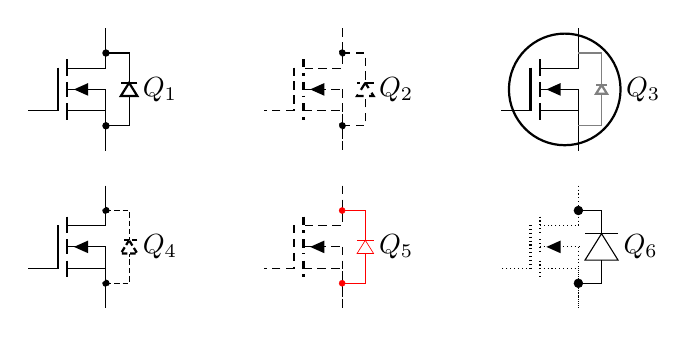
\begin{tikzpicture}[red solid thin bodydiode/.style={bodydiode,
        circuitikz/transistor bodydiode/dash=none,
        circuitikz/transistor bodydiode/color=red,
        circuitikz/transistor bodydiode/relative thickness=0.3}]
    \draw (0,0) node (mosfet1) [nigfete,anchor=D,bodydiode] {$Q_1$};
    \draw[densely dashed]  (3,0) node (mosfet1) [nigfete,anchor=D,bodydiode] {$Q_2$};
    \draw (6,0) node (mosfet1) [nigfete,anchor=D,bodydiode, tr circle,
        circuitikz/transistor bodydiode/color=gray,
        circuitikz/transistor bodydiode/scale=0.2,
        circuitikz/transistor bodydiode/dot scale=0] {$Q_3$};
    \draw (0,-2) node (mosfet1) [nigfete,anchor=D,bodydiode,
        circuitikz/transistor bodydiode/dash={{2pt}{1pt}}]  {$Q_4$};
    \draw[densely dashed]  (3,-2) node (mosfet1) [nigfete,anchor=D,
        red solid thin bodydiode] {$Q_5$};
    \ctikzset{transistor bodydiode/relative thickness=.5,
        transistor bodydiode/scale=0.6}% from now on, in scope
    \draw[densely dotted] (6,-2) node (mosfet1) [nigfete,anchor=D,bodydiode,
          circuitikz/transistor bodydiode/dash=none,
          circuitikz/transistor bodydiode/dot scale=1] {$Q_6$};
    \path (7,0); %% adjust bounding box (node text is outside it!)
\end{tikzpicture}
\end{LTXexample}

\subsubsection{Transistors anchors}

For \textsc{nmos}, \textsc{pmos}, \textsc{nfet}, \textsc{nigfete}, \textsc{nigfetd}, \textsc{pfet}, \textsc{pigfete}, and \textsc{pigfetd}  transistors  one has \texttt{base}, \texttt{gate}, \texttt{source} and \texttt{drain} anchors (which can be abbreviated with \texttt{B}, \texttt{G}, \texttt{S} and \texttt{D}):

\begin{LTXexample}[varwidth=true]
\begin{circuitikz} \draw
  (0,0) node[nmos] (mos)  {}
  (mos.gate) node[anchor=east] {G}
  (mos.drain) node[anchor=south] {D}
  (mos.source) node[anchor=north] {S}
;\end{circuitikz}
\end{LTXexample}

\begin{LTXexample}[varwidth=true]
\begin{circuitikz} \draw
  (0,0) node[pigfete] (pigfete)  {}
  (pigfete.G) node[anchor=east] {G}
  (pigfete.D) node[anchor=north] {D}
  (pigfete.S) node[anchor=south] {S}
  (pigfete.bulk) node[anchor=west] {Bulk}
;\end{circuitikz}
\end{LTXexample}

Similarly \textsc{njfet} and \textsc{pjfet} have  \texttt{gate}, \texttt{source} and \texttt{drain} anchors (which can be abbreviated with  \texttt{G}, \texttt{S} and \texttt{D}):

\begin{LTXexample}[varwidth=true]
\begin{circuitikz} \draw
  (0,0) node[pjfet] (pjfet)  {}
  (pjfet.G) node[anchor=east] {G}
  (pjfet.D) node[anchor=north] {D}
  (pjfet.S) node[anchor=south] {S}
;\end{circuitikz}
\end{LTXexample}

For \textsc{npn}, \textsc{pnp}, \textsc{nigbt} and \textsc{pigbt} transistors, the anchors are  \texttt{base}, \texttt{emitter} and \texttt{collector} anchors (which can be abbreviated with \texttt{B}, \texttt{E} and \texttt{C}):

\begin{LTXexample}[varwidth=true]
\begin{circuitikz} \draw
  (0,0) node[npn] (npn)  {}
  (npn.base) node[anchor=east] {B}
  (npn.collector) node[anchor=south] {C}
  (npn.emitter) node[anchor=north] {E}
;\end{circuitikz}
\end{LTXexample}

\begin{LTXexample}[varwidth=true]
\begin{circuitikz} \draw
  (0,0) node[pigbt] (pigbt)  {}
  (pigbt.B) node[anchor=east] {B}
  (pigbt.C) node[anchor=north] {C}
  (pigbt.E) node[anchor=south] {E}
;\end{circuitikz}
\end{LTXexample}


Notice that the geographical anchors of transistors are \emph{not} affected by either the bodydiode and the circle options; the label text is also outside of them. This is to permit aligning the components independently from those features. On the other hand, this can sometimes create problems because that element is outside the bounding box automatically calculated by \TikZ{}.

The exception is the \texttt{right} anchor which, when a circle is present, indicates the edge of the circle itself (since \texttt{v1.3.2})

{\geolrcoord{npn}  \geolrcoord{npn, bodydiode} \geolrcoord{npn, bodydiode, tr circle}}


All transistors, except the multi-terminal \texttt{bjtnpn} and \texttt{bjtpnp}, (since \texttt{0.9.6}) have internal nodes on the terminal corners, called \texttt{inner up}  and \texttt{inner down}; you do not normally need them, but they are here for special applications:

\begin{LTXexample}[varwidth=true]
\begin{circuitikz}
    \node [npn](A) at(0,2) {};
    \node [pmos](B) at(0,0) {};
    \foreach \e in {A, B}
        \foreach \a in {inner up, inner down} {
            \node[red, circle, inner sep=1pt, draw]
            at (\e.\a) {};
            \node [right, font=\tiny, blue]
            at (\e.\a) {\a};
        }
\end{circuitikz}
\end{LTXexample}

Additionally, you can access the position for the flyback diodes and possibly snubbers as shown in~\ref{sec:bodydiodes-anchor}.

\begin{quote}
\showanchors{npn}{}(body C in/45/0.4,  body E in/-45/0.4, body C out/0/0.4, body E out/0/0.4)
\showanchors{npn, bodydiode}{}(body C in/45/0.4,  body E in/-45/0.4, body C out/0/0.4, body E out/0/0.4)
\showanchors{pnp}{}(body C in/-45/0.4,  body E in/45/0.4, body C out/0/0.4, body E out/0/0.4)
\end{quote}

Transistor circles also have several anchors on them:
\begin{quote}
\showanchors{npn, tr circle}{}(circle center/-135/0.6, circle top/90/0.3, circle left/180/0.2, circle right/0/0.2, circle bottom/-90/0.3, circle C/45/0.2, circle E/-45/0.2)
\showanchors{pigfete, bodydiode, tr circle}{}(circle center/-135/0.6, circle top/90/0.3, circle left/180/0.2, circle right/0/0.2, circle bottom/-90/0.3, circle C/-45/0.2, circle E/45/0.2)
\end{quote}

The multi-terminal transistors have all the geographical anchors; note though that the \texttt{center} anchor is not the geometrical center of the component, but the logical one (at the same height as the base).
The additional anchors \texttt{vcenter} (vertical geometric center of the collector--emitter zone) and \texttt{gcenter} (graphical center) are provided, as shown in the following picture. They have no bodydiode anchors nor \texttt{inner \emph{up/down}} ones.

\begin{quote}
\geocoord{bjtnpn, collectors=1, emitters=2}
\showanchors{bjtpnp, collectors=4, emitters=1, bjt pins width=0.6}{}(north/90/0.4,  east/0/0.4, south/-90/0.4, west/180/0.4, center/120/0.3, vcenter/0/0.4, gcenter/-120/0.4, cbase/-60/0.6)
\end{quote}

A complete example of multiple terminal transistor application is the following PNP double current mirror circuit.

\begin{LTXexample}[varwidth=true]
\begin{circuitikz}
    \ctikzset{transistors/arrow pos=end}
    \draw (0,0) node[bjtpnp, xscale=-1](Q1){%
        \scalebox{-1}[1]{Q1}};
    \draw (Q1.B) node[bjtpnp, anchor=B, collectors=2]
        (Q2){Q2} (Q1.B) node[circ]{};
    \draw (Q1.E) node[circ]{} node[vcc]{} (Q2.E)
        node[vcc]{} (Q1.E) -| (Q1.B);
    \draw (Q1.C) to[R, l_=$R_0$, f=$I_0$] ++(0,-3.5)
        node[ground](GND){};
    \draw (Q2.C) -- ++(0,-0.5) coordinate(a);
    \draw (Q2.C1) -- ++(1,0) coordinate(b) -- (b|-a);
    \draw (a) ++(0,-0.1) node[flowarrow, rotate=-90,
        anchor=west]{\rotatebox{90}{$I_0$}};
    \draw (b|-a) ++(0,-0.1) node[flowarrow, rotate=-90,
        anchor=west]{\rotatebox{90}{$I_0$}};
    \path (b) ++(0.5,0); % bounding box adjust
\end{circuitikz}
\end{LTXexample}


Here is one composite example (please notice that the \texttt{xscale=-1} style would also reflect the label of the transistors, so here a new node is added and its text is used, instead of that of \texttt{pnp1}):

\begin{LTXexample}[varwidth=true]
  \begin{circuitikz} []\draw
  (0,0) node[pnp] (pnp2) {Q2}
  (pnp2.B) node[pnp, xscale=-1, anchor=B] (pnp1) {}
  (pnp1) node[left, inner sep=0pt] {Q1}
  (pnp1.C) node[npn, anchor=C] (npn1) {Q3}
  (pnp2.C) node[npn, xscale=-1, anchor=C] (npn2)
    {\scalebox{-1}[1]{Q4}}
  (pnp1.E) -- (pnp2.E)  (npn1.E) -- (npn2.E)
  (pnp1.B) node[circ] {} |- (pnp2.C) node[circ] {}
;\end{circuitikz}
\end{LTXexample}

Notice that the text labels of transistors are outside the bounding box of the component (that is, the set of geographical anchors). If it is a problem, use a separate text node to set the transistor's label.
Of course, transistors like other components can be reflected vertically:

\begin{LTXexample}[varwidth=true]
\begin{circuitikz} \draw
  (0,0) node[pigfete, yscale=-1] (pigfete)  {}
  (pigfete.bulk) node[anchor=west] {Bulk}
  (pigfete.G) node[anchor=east] {G}
  (pigfete.D) node[anchor=south] {D}
  (pigfete.S) node[anchor=north] {S}
;\end{circuitikz}
\end{LTXexample}

Finally, double-gated components (MOSes, FETs, IGBTs) have an extra anchor \texttt{centergap} positioned in the middle of the ``gate capacitor'' or base.
\begin{LTXexample}[varwidth=true]
    \begin{circuitikz}
        \node [nmos](A) at (0,3) {};
        \node [nfet](B) at (0,1.5) {};
        \node [pigbt](C) at (0,0) {};
        \foreach \myn in {A, B, C}
            \draw[color=red] (\myn.centergap)
                node[ocirc]{} -- ++(1,0)
                node[right, font=\tiny]{centergap};
    \end{circuitikz}
\end{LTXexample}

For UJT transistors anchors, see section~\ref{sec:ujt}.


\subsubsection{Transistor paths}\label{sec:transasbip}

For syntactical convenience standard transistors (not multi-terminal ones) can be placed using the normal path notation used for bipoles. The transistor type can be specified by  simply adding a ``T'' (for transistor) in front of the node name of the transistor. It will be placed with the base/gate orthogonal to the direction of the path:

\begin{LTXexample}[varwidth=true]
\begin{circuitikz} \draw
  (0,0) node[njfet] {1}
  (-1,2) to[Tnjfet=2] (1,2)
    to[Tnjfet=3, mirror] (3,2)
;\end{circuitikz}
\end{LTXexample}

Access to the gate and/or base nodes can be gained by naming the transistors with the \texttt{n} or \texttt{name} path style:
\begin{LTXexample}[varwidth=true]
\begin{circuitikz} \draw[yscale=1.1, xscale=.8]
  (2,4.5) -- (0,4.5) to[Tpmos=p1, n=p1] (0,3)
     to[Tnmos=n1, n=n1] (0,1.5)
     to[Tnmos=n2, n=n2] (0,0) node[ground] {}
  (2,4.5) to[Tpmos=p2,n=p2] (2,3) to[short, -*] (0,3)
  (p1.G) -- (n1.G) to[short, *-o] ($(n1.G)+(3,0)$)
  (n2.G) ++(2,0) node[circ] {} -| (p2.G)
  (n2.G) to[short, -o] ($(n2.G)+(3,0)$)
  (0,3) to[short, -o] (-1,3)
;\end{circuitikz}
\end{LTXexample}

Transistors used in path are fully path-style components, so to flip and rotate them you should use  \texttt{mirror} and \texttt{invert} as shown in section~\ref{sec:mirror-flip-path}.

Transistor paths have the possibility to use the poles syntax (see section~\ref{sec:bipole-nodes}) but they have \textbf{no} voltage, current, flow, annotation options.
Also, the positioning of the labels is very simple and is not foolproof for all rotations; if you need to control them more please name the node and position them by hand, or use the more natural node style for transistors.

The \texttt{name} property is available also for bipoles; this is useful mostly for triac, potentiometer and thyristor (see~\ref{sec:othertrip}).



\subsection{Electronic Tubes}

Electronic tubes, also known as vacuum tubes, control current flow between electrodes.  They come in many different flavours.
\small{Contributed by J. op den Brouw (\texttt{J.E.J.opdenBrouw@hhs.nl}).}

\begin{groupdesc}
	\circuitdesc*{diodetube}{Tube Diode}{}(anode/90/0.2, cathode/-90/0.2 )
	\circuitdesc*{triode}{Triode}{}(anode/90/0.2, cathode/-90/0.2, control/180/0.2 )
	\circuitdesc*{tetrode}{Tetrode}{}(anode/90/0.2, cathode/-90/0.2, control/190/0.2,screen/170/0.2 )
	\circuitdesc*{pentode}{Pentode}{}(anode/90/0.2, cathode/-90/0.2, control/190/0.2,screen/180/0.2,suppressor/170/0.2 )
\end{groupdesc}

Some pentodes have the suppressor grid internally connected to the control grid, which saves a pin on the tube's housing.

\begin{groupdesc}
	\circuitdesc*{pentode suppressor to cathode}{Pentode with suppressor grid connected to cathode}{}( anode/90/0.2, cathode/-90/0.2, control/190/0.2,screen/180/0.2 )
\end{groupdesc}

Note that the \verb|diodetube| is used as component name to avoid clashes with the semiconductor diode.
Normally, the filament is not drawn. If you want a filament, put the \verb|filament| option in the node description:

\begin{groupdesc}
	\circuitdesc*{diodetube,filament}{Tube Diode}{}(anode/90/0.2, filament 1/-135/0.2, filament 2/-45/0.2 )
\end{groupdesc}

Sometimes, you don't want the cathode to be drawn (but you do want the filament). Use the \verb|nocathode| option in the node description:

\begin{groupdesc}
	\circuitdesc*{diodetube,filament,nocathode}{Tube Diode}{}(anode/90/0.2 )
\end{groupdesc}

If you want a full cathode to be drawn, use the \verb|fullcathode| option in the node description. You can then use the anchors \verb|cathode 1| and \verb|cathode 2|.

\begin{groupdesc}
	\circuitdesc*{diodetube,fullcathode}{Tube Diode}{}(anode/90/0.2, cathode 1/-135/0.2, cathode 2/-45/0.2 )
\end{groupdesc}

\subsubsection{Tubes customization}

The tubes can be scaled using the key \texttt{tubes/scale}, default \texttt{1.0}. In addition, they are
fully configurable, and the attributes are described below:

\begin{tabular}{l | l | l}

  Key & Default value & Description\\
  \hline
  \verb|tubes/scale| & \verb|1|                    & scale factor                 \\
  \verb|tubes/width| & \verb|1|                    & relative width               \\
  \verb|tubes/height| & \verb|1.4|                 & relative height              \\
  \verb|tubes/tube radius| & \verb|0.40|           & radius of tube circle        \\
  \verb|tubes/anode distance| & \verb|0.40|        & distance from center         \\
  \verb|tubes/anode width| & \verb|0.40|           & width of an anode/plate      \\
  \verb|tubes/grid protrusion| & \verb|0.25|       & distance from center         \\
  \verb|tubes/grid dashes| & \verb|5|              & number of grid dashes        \\
  \verb|tubes/grid separation| & \verb|0.2|        & separation between grids     \\
  \verb|tubes/grid shift| & \verb|0.0|             & y shift of grids from center \\
  \verb|tubes/cathode distance| & \verb|0.40|      & distance from grid           \\
  \verb|tubes/cathode width| & \verb|0.40|         & width of a cathode           \\
  \verb|tubes/cathode corners| & \verb|0.06|       & corners of the cathode wire  \\
  \verb|tubes/cathode right extend| & \verb|0.075| & extension at the right side  \\
  \verb|tubes/filament distance| & \verb|0.1|      & distance from cathode        \\
  \verb|tubes/filament angle| & \verb|15|          & angle from the centerpoint   \\
\end{tabular}

Conventionally, the model of the tube is indicated at the \verb|east| anchor:

\begin{LTXexample}[varwidth]
\ctikzset{tubes/width=1.4}
\ctikzset{tubes/height=1}

\begin{circuitikz}
\draw (0,0) node[triode] (Tri) {};
\draw  (Tri.east) node[right] {12AX7};
\end{circuitikz}
\end{LTXexample}

Example triode amplifier:

\begin{lstlisting}
\begin{circuitikz}
\draw (0,0) node (start) {}
                to[sV=$V_i$] ++(0,2+\ctikzvalof{tubes/height})
                to[C=$C_i$] ++(2,0) coordinate(Rg)
                to[R=$R_g$] (Rg |- start)
(Rg)            to[short,*-] ++(1,0)
                node[triode,anchor=control] (Tri) {} ++(2,0)
(Tri.cathode)   to[R=$R_c$,-*] (Tri.cathode |- start)
(Tri.anode)     to [R=$R_a$] ++(0,2)
                to [short] ++(3.5,0) node(Vatop) {}
                to [V<=$V_a$] (Vatop |- start)
                to [short] (start)
(Tri.anode)     ++(0,0.2) to[C=$C_o$,*-o] ++(2,0)
(Tri.cathode)   ++(0,-0.2) to[short,*-] ++(1.5,0) node(Cctop) {}
                to[C=$C_c$,-*] (start -| Cctop)
;
\draw[red,thin,dashed] (Tri.north west) rectangle (Tri.south east);
\draw (Tri.east) node[right] {12AX7};
\end{circuitikz}
\end{lstlisting}

\begin{circuitikz}[scale=0.7, transform shape]
\draw (0,0) node (start) {}
                to[sV=$V_i$] ++(0,2+\ctikzvalof{tubes/height})
                to[C=$C_i$] ++(2,0) coordinate(Rg)
                to[R=$R_g$] (Rg |- start)
(Rg)            to[short,*-] ++(1,0)
                node[triode,anchor=control] (Tri) {} ++(2,0)
(Tri.cathode)   to[R=$R_c$,-*] (Tri.cathode |- start)
(Tri.anode)     to [R=$R_a$] ++(0,2)
                to [short] ++(3.5,0) node(Vatop) {}
                to [V<=$V_a$] (Vatop |- start)
                to [short] (start)
(Tri.anode)     ++(0,0.2) to[C=$C_o$,*-o] ++(2,0)
(Tri.cathode)   ++(0,-0.2) to[short,*-] ++(1.5,0) node(Cctop) {}
                to[C=$C_c$,-*] (start -| Cctop)
;
\draw[red,thin,dashed] (Tri.north west) rectangle (Tri.south east);
\draw (Tri.east) node[right] {12AX7};
\end{circuitikz}

\subsubsection{Tubes anchors}

Apart from the geographic anchors, which take into account the leads of the components, you have several anchors on the border:
\begin{quote}
\geolrcoord{pentode, scale=0.8}
\geolrcoord{triode, circuitikz/tubes/width=1.4, circuitikz/tubes/height=1, scale=0.8}
\geolrcoord{triode, circuitikz/tubes/width=1, circuitikz/tubes/height=1, scale=0.8}

\showanchors{pentode, circuitikz/tubes/height=1.8}{}(%
tube top/90/0.3, tube left/180/0.2, tube right/0/0.2, tube bottom/-90/0.3,
tube top right/30/0.2, tube top left/150/0.4, tube bottom right/-45/0.4, tube bottom left/-150/0.2,
tube top center/75/0.5, tube bottom center/-105/0.5)
\showanchors{pentode,circuitikz/tubes/width=2.6, circuitikz/tubes/tube radius=0.3}{}(%
tube top/90/0.5, tube left/160/0.5, tube right/0/0.2, tube bottom/-90/0.6,
tube top right/70/0.4, tube top left/150/0.4, tube bottom right/-45/0.4, tube bottom left/-120/0.4,
tube right center/30/0.4, tube left center/-120/0.4)
\end{quote}

\subsubsection{Partially drawn tube borders}\label{sec:partial-tube-borders}

In some circuits, tubes are drawn with partial or dashed border (to convey the meaning of several active components encased in the same physical tube). To achieve this effect, you can use the \texttt{tubes/partial border}\footnote{Suggested by \href{https://github.com/circuitikz/circuitikz/issues/602}{Jether Fernandes Reis}, implemented by Romano in \texttt{v1.5.2}.} key (default \texttt{none}). This key can be set to \texttt{none}, or must be a sequence of \textbf{exactly} 6 numbers, which can have value \texttt{0}, \texttt{1}, or \texttt{2}. Each number defines the style of a part of the border to be not drawn, solid or dashed respectively.

The part of the border are numbered from 1 to 6 as shown below:
\begin{quote}
\begin{circuitikz}[circuitikz/tubes/fill=cyan!20,
            circuitikz/tubes/partial borders=121212]
            \draw (0,0) node[pentode,anchor=control](V){};
            \draw (4,0) node[pentode,anchor=control,
            circuitikz/tubes/width=1.4,
            circuitikz/tubes/height=1](H){};
            \draw[red, font=\ttfamily\small\bfseries]
                ([shift={(-.2,-.2)}]V.ne) node{1}
                ([shift={(.1,0)}]V.e) node{2}
                ([shift={(-.2,.2)}]V.se) node{3}
                ([shift={(.2,.2)}]V.sw) node{4}
                ([shift={(-.1,0)}]V.w) node{5}
                ([shift={(.2,-.2)}]V.nw) node{6}
                ([shift={(.2,-.2)}]H.nw) node{1}
                ([shift={(0,.1)}]H.n) node{2}
                ([shift={(-.2,-.2)}]H.ne) node{3}
                ([shift={(-.2,.2)}]H.se) node{4}
                ([shift={(0,-.1)}]H.s) node{5}
                ([shift={(.2,.2)}]H.sw) node{6}
                ;
    \end{circuitikz}
\end{quote}
(notice that the straight parts, if they exist, are numbered \texttt{2} and \texttt{5} in both tubes, vertical or horizontal).

The dashed line pattern can be changed by setting the key \texttt{tubes/partial border dash} (default \verb|{{2pt}{2pt}}|).\footnote{Follows the syntax of the pattern sequence \texttt{\textbackslash pgfsetdash} --- see \TikZ{} manual for details; phase is always zero. Basically you pass pairs of dash-length -- blank-length dimensions, see the examples.} Be careful with the extra set of braces here.

\begin{LTXexample}[varwidth=true, basicstyle=\small\ttfamily]
\begin{circuitikz}[circuitikz/tubes/fill=cyan!20,
        circuitikz/tubes/partial borders=012012]
        \draw (0,0) node[pentode]{};
        \draw (2,0) node[pentode,
        circuitikz/tubes/width=1.4,
        circuitikz/tubes/height=1]{};
        \draw (1,-2) node[triode,
        circuitikz/tubes/height=1,
        circuitikz/tubes/partial border dash=%
            {{3pt}{1pt}{1pt}{1pt}}]{};
\end{circuitikz}
\end{LTXexample}



\subsubsection{Other tubes-like components}

The \texttt{magnetron} and \texttt{dynode} shapes will also scale with \texttt{tubes/scale}.

\begin{groupdesc}
    \circuitdesc*{magnetron}{Magnetron}{}( anode/-90/0.2, cathode1/135/0.2,
    cathode2/45/0.2, left/180/0.2, right/0/0.2, top/90/0.4 )
    \circuitdesc{dynode}{Dynode\footnotemark}{D}( top/90/0.1, bottom/180/0.3, left/180/0.3, right/0/0.3, center/0/0.3, arc/-30/0.4, top right/30/0.2, top left/150/0.2 )
    \footnotetext{Suggested by the user \texttt{ferdymercury} on \href{https://github.com/circuitikz/circuitikz/issues/469}{GitHub}.}
\end{groupdesc}

\begin{LTXexample}[varwidth=true]
\begin{circuitikz}
\draw (0,-2)node[rground](gnd){} to[voltage source,v<={HV}]++(0,3)--++(1,0)to[V,n=DC]++(2,0);
\draw (2,-1) node[magnetron,scale=1](magn){};
\draw (DC.left)++(-0.2,0)to [short,*-] ++(0,-1) to [short] (magn.cathode1);
\draw (DC.right)++(0.2,0)to [short,*-] ++(0,-1) to [short] (magn.cathode2);
\draw (magn.anode) to [short] (magn.anode|-gnd) node[rground]{};
\draw (magn.cathode1)node[above]{$1$};
\draw (magn.cathode2)node[above]{$2$};
\draw[->](magn.east) --++(1,0)node[right]{$RF_{out}$};
\end{circuitikz}
\end{LTXexample}


\paragraph{Dynode customization.}
The dynode element can be heavily customized. The parameters are the following (all of them under the \verb|\ctikzset| family \texttt{monopoles/dynode}):

\begin{center}
\begin{tabular}{>{\ttfamily}l>{\ttfamily}rp{0.75\linewidth}}
    \toprule
    parameter & default & description \\
    \midrule
    width & \ctikzvalof{monopoles/dynode/width} &  Total width (relative to the base length) measured at the arc width.\\
    height & \ctikzvalof{monopoles/dynode/height} &  Total height (same units as width).\\
    arc angle & \ctikzvalof{monopoles/dynode/arc angle} &  Angle (from the horizontal, going down) where the arc starts. A value of \texttt{90} don't plot any arc, \texttt{0} plots a semicircle. To avoid artifacts, use a value between \texttt{-60} and \texttt{90}; the arc horizontal size is always equal to the \texttt{width}.\\
    arc pos & \ctikzvalof{monopoles/dynode/arc pos} &  Vertical position (relative to the height) of the arc center. \\
    top width & \ctikzvalof{monopoles/dynode/top width} &  Relative width of the top bar; a value of \texttt{1} means full width, \texttt{0} means no bar.\\
    \bottomrule
\end{tabular}
\end{center}


\begin{LTXexample}[varwidth=true]
\begin{circuitikz}[american] \ctikzset{tubes/thickness=4}
    \draw (0,0) to[R] (2,0) node[dynode]{} to[R,-*] (4,0);
    \ctikzset{monopoles/dynode/.cd,
        arc angle=0, arc pos=0.7, top width=0.5}
    \draw (4,0) node[dynode]{};
\end{circuitikz}
\end{LTXexample}

You can use styles and the parameters to create different types of electrodes:

\begin{LTXexample}[varwidth=true]
\begin{circuitikz}[american] \ctikzset{tubes/thickness=4}
    \tikzset{anode/.style={dynode,
            circuitikz/monopoles/dynode/arc angle=90},
        photocatode/.style={dynode,
            circuitikz/monopoles/dynode/arc pos=1,
            circuitikz/monopoles/dynode/top width=0},
    }
    \draw (0,0) node[dynode]{} (1,0) node[anode]{}
           (2,0) node[photocatode]{};
\end{circuitikz}
\end{LTXexample}


\subsection{RF components}\label{sec:RF}

For the RF components, similarly to the grounds and supply rails, the \texttt{center} anchor is put on the connecting point of the symbol, so that you can use them directly in a \texttt{path} specification.

Notes that in the transmission and receiving antennas, the ``waves'' are outside the geographical anchors.

\begin{groupdesc}
    \circuitdesc*{bareantenna}{Bare Antenna}{A}( top/90/0.1, bottom/180/0.3, left/180/0.3, right/45/0.3, center/0/0.3 )
    \circuitdesc*{dinantenna}{DIN antenna\footnotemark}{A}(left/135/0.6, right/45/0.6, center/-45/0.6)
    \footnotetext{Since 1.5.0, suggested by \href{https://github.com/circuitikz/circuitikz/issues/621}{GitHUb user myzinsky}}
    \circuitdesc*{bareTXantenna}{Bare TX Antenna}{Tx}( top/90/0.1, center/180/0.3, waves/90/0.3 )
    \circuitdesc*{bareRXantenna}{Bare RX Antenna}{Rx}( top/90/0.1, center/0/0.3, waves/90/0.3 )
    \circuitdesc{waves}{Waves}{}( north/90/0.4, north east/45/0.4, east/-45/0.4, south east/-45/0.4,
    south/-90/0.4, south west/-135/0.4, west/180/0.4, north west/135/0.4,
    left/135/0.2, top/45/0.2, right/45/0.2, bottom/-45/0.2 )
    \circuitdescbip*{mstline}{Microstrip transmission line\footnotemark}{}(left/135/0.2, right/45/0.2, center/-90/0.3)
    \circuitdesc*{mslstub}{Microstrip linear stub}{text}(left/135/0.2, right/45/0.2, center/-45/0.3)
    \circuitdesc*{msport}{Microstrip port}{T}(left/135/0.2, right/45/0.2, center/-45/0.3)
    \circuitdesc*{msrstub}{Microstrip radial stub}{}(left/135/0.2, right/45/0.2, center/-45/0.3)
    \footnotetext{These four components were suggested by \texttt{@tcpluess} on GitHub}
    \circuitdesc{antenna}{Legacy antenna (with tails)}{}( center/0/0.3 )
    \circuitdesc{rxantenna}{Legacy receiving antenna (with tails)}{}
    \circuitdesc{txantenna}{Legacy transmitting antenna (with tails)}{}
    \circuitdesc*{tlinestub}{Transmission line stub}{}
    \circuitdescbip*[tline]{TL}{Transmission line}{transmission line, tline}(left/135/0.3, right/45/0.3, top left/90/0.2, top right/90/0.4, bottom left/-90/0.4, bottom right/-70/0.3, center right/-30/0.2, center left/-160/0.2)
    \circuitdescbip[tline]{TL, bipoles/tline/bare=true}{Transmission line without wires (notice that if you fill it, the fill will overwrite the exiting wire)}{transmission line, tline}(left/90/0.3, right/90/0.3)
    \circuitdesc{match}{match}{}
\end{groupdesc}

\subsubsection{RF elements customization}

The RF elements can be scaled using the key \texttt{RF/scale}, default \texttt{1.0}.

\subsubsection{Microstrip customization}

The microstrip linear components' (\texttt{mstline}, \texttt{mslstub}, \texttt{msport}) heights can be changed by setting the parameter \texttt{bipoles/mstline/height} (for the three of them, default 0.3). The widths are specified in \texttt{bipoles/mstline/width} for the first two and by \texttt{monopoles/msport/width} for the port (defaults: 1.2, 0.5).

For the length parameter of the transmission line there is a shortcut in the form of the direct parameter \texttt{mstlinelen}.

\begin{LTXexample}[varwidth=true, pos=t]
\begin{circuitikz}
    \draw (0,0) node[msport, right, xscale=-1]{}
    to[mstline, -o]  ++(3,0) coordinate(there)
    to[mstline, mstlinelen=2, l=longer, o-*]  ++(4,0)
        coordinate(here) -- ++(0.5,0) node[mslstub, fill=yellow]{stub}
        (here) -- ++(0,0.5) node[mslstub, rotate=90, mstlinelen=0.5]{short};
        \draw (there) to[short, o-]  ++(0, 0.5) node[msrstub]{};
        \draw (here) -- ++(0, -0.5) node[msrstub, yscale=-1]{};
\end{circuitikz}
\end{LTXexample}

The legacy \texttt{tline} can be used as in the following example. You can change the length with the key  \texttt{bipoles/tline/width} (default \texttt{0.6}). The ``bare'' version, which differs only for the small line on the visible ellipse, and activated with the boolean key \texttt{\dots/bare}, is useful as a substitute for \texttt{tlinestub} (with more flexibility).

\begin{LTXexample}[varwidth=true]
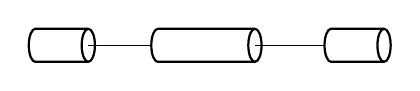
\begin{tikzpicture}[]
    \tikzset{bare tl/.style={tlineshape,
    circuitikz/bipoles/tline/bare=true}}
    \draw (0,0) node[bare tl](A){} (A.right)
        to[TL, bipoles/tline/width=1] ++(3,0)
        node[bare tl, anchor=left]{};
\end{tikzpicture}
\end{LTXexample}

\subsection{Electro-Mechanical Devices}

The internal part of the motor and generator are, by default, filled with white (to avoid compatibility problems with older versions of the package).

\begin{groupdesc}
    \circuitdesc*{elmech}{Motor}{M}(bottom/-90/0.2, left/180/0.2, right/0/0.2, top/90/0.4, 45/45/0.2)
    \circuitdesc*{elmech}{Generator}{G}(block down right/0/0.2, block north east/0/0.2)
\end{groupdesc}

\subsubsection{Electro-Mechanical Devices anchors}

Apart from the standard geographical anchors, \texttt{elmech} has the border anchors (situated on the inner circle) and the following anchors on the ``block'':

\begin{quote}
\begin{circuitikz}
    \def\coordx(#1)[#2:#3]#4{node[circle, #4, draw, inner sep=1pt,pin={[#4, inner sep=0.5pt, font=\scriptsize, pin distance=#2cm, pin edge={#4, }]#3:#1}](#1){}}
    \node [elmech](T) at(0,0) {A};
    \foreach \a/\d/\t in {block north east/0.2/45, block south east/0.2/-45,
        block south west/0.2/-135, block north west/0.1/135, 150/0.1/150,
        180/0.1/180, 210/0.1/210, 60/0.4/-15, -60/0.4/15}
    \path (T.\a) \coordx(\a)[\d:\t]{red};
    \node [elmech](T) at(6,0) {B};
    \foreach \a/\d/\t in {block up right/0.2/45, block down right/0.2/-45,
        block down left/0.2/-135, block up left/0.1/135, north/0.3/90,
        south/0.3/-90, east/0.3/0, west/0.3/180}
    \path (T.\a) \coordx(\a)[\d:\t]{red};
\end{circuitikz}
\end{quote}


\begin{LTXexample}[varwidth=true]
\begin{circuitikz}
\draw (2,0) node[elmech](motor){M};
\draw (motor.north) |-(0,2) to [R] ++(0,-2) to[dcvsource]++(0,-2) -| (motor.bottom);
\draw[thick,->>](motor.right)--++(1,0)node[midway,above]{$\omega$};
\end{circuitikz}
\end{LTXexample}
\begin{LTXexample}[varwidth=true]
\begin{circuitikz}
\draw (2,0) node[elmech](motor){};
\draw (motor.north) |-(0,2) to [R] ++(0,-2) to[dcvsource]++(0,-2) -| (motor.bottom);
\draw[thick,->>](motor.center)--++(1.5,0)node[midway,above]{$\omega$};
\end{circuitikz}
\end{LTXexample}

The symbols can also be used along a path, using the transistor-path-syntax(\texttt{T} in front of the shape name, see section \ref{sec:transasbip}). Don't forget to use parameter $n$ to name the node and get access to the anchors:

\begin{LTXexample}[varwidth=true]
\begin{circuitikz}
\draw (0,0) to [Telmech=M,n=motor] ++(0,-3) to [Telmech=M] ++(3,0) to [Telmech=G,n=generator] ++(0,3) to [R] (0,0);
\draw[thick,->>](motor.left)--(generator.left)node[midway,above]{$\omega$};
\end{circuitikz}
\end{LTXexample}



\subsection{Double bipoles (transformers)}\label{sec:transformers}

Transformers automatically use the inductor shape currently selected. These are the three possibilities:
\begin{groupdesc}
    \ctikzset{inductor=cute}
    \circuitdesc{transformer}{Transformer (cute inductor)}{$T_1$}( A1/180/0.1,
    A2/180/0.1, B1/0/0.1, B2/0/0.1, north/45/0.4,
    inner dot A1/-135/0.2, inner dot A2/135/0.2, inner dot B1/-45/0.1,
    inner dot B2/45/0.1 )
    \ctikzset{inductor=american}
    \circuitdesc{transformer}{Transformer (american inductor)}{}( %
    outer dot A1/180/0.2, outer dot A2/180/0.2,
    outer dot B1/0/0.2, outer dot B2/0/0.2 )
    \ctikzset{inductor=european}
    \circuitdesc{transformer}{Transformer (european inductor)}{}
    \circuitdesc*{gyrator}{Gyrator}{}
\end{groupdesc}


Transformers with core are also available:
\begin{groupdesc}
    \ctikzset{inductor=cute}
    \circuitdesc{transformer core}{Transformer  core (cute inductor)}{}
    \ctikzset{inductor=american}
    \circuitdesc{transformer core}{Transformer core (american inductor)}{}
    \ctikzset{inductor=european}
    \circuitdesc{transformer core}{Transformer core (european inductor)}{}
    \ctikzset{inductor=cute} % reset default
\end{groupdesc}

You can also build generic double bipoles\footnote{The idea of generic double bipoles was originated by user \href{https://github.com/circuitikz/circuitikz/issues/641}{erwindenboer on GitHub}.} (although it's often better to use subcircuits in this case; see section~\ref{sec:subcircuits}).

\begin{groupdesc}
    \circuitdesc{double bipole}{Generic double bipole (configurable components)}{$A_v$}(north/45/0.4, center/-90/0.6, east/45/0.2)[L.south/180/0.2, R.west/-45/0.2]
    \ctikzset{double bipole L=fulllediodeshape, double bipole R=emptydiodeshape, double bipole R invert, diodes/scale=0.6}
    \circuitdesc{double bipole}{Generic double bipole (this specific configuration is shown in section~\ref{sec:doublebipoles})}{$A_v$}(north/45/0.4, center/-90/0.6, east/45/0.2)[L.south/180/0.2, R.west/-45/0.2]
\end{groupdesc}

\subsubsection{Transformer anchors}

All the double bipoles/quadrupoles have the four anchors, two for each port.
The first port, to the left, is port \texttt{A}, having the anchors \texttt{A1} (up) and \texttt{A2} (down); same for port \texttt{B}.

They also expose the \texttt{base} anchor, for labeling, and anchors for setting dots or signs to specify polarity.
The set of anchors, to which the standard ``geographical'' \texttt{north}, \texttt{north east}, etc. is here:

\medskip
\begin{quote}
\begin{circuitikz}[cute inductors,
    ]
    \def\coordx(#1)[#2:#3]#4{node[circle, #4, draw, inner sep=1pt,pin={[#4, overlay, inner sep=0.5pt, font=\scriptsize, pin distance=#2cm, pin edge={#4, overlay,}]#3:#1}](#1){}}
    \foreach \comp/\pos/\case in {%
                            transformer/0/0%
                            ,transformer core/4/1%
                            ,gyrator/8/2%
                            }{
        \draw (\pos, 0) node[\comp](T){};
        \ifcase\case
            \foreach \a/\d/\t in {inner dot A1/0.2/75, inner dot A2/0.2/-75, inner dot B1/0.1/-45, inner dot B2/0.1/45}
            \path (T.\a) \coordx(\a)[\d:\t]{red};
        \or
            \foreach \a/\d/\t in {outer dot A1/0.2/75, outer dot A2/0.2/-75, outer dot B1/0.2/-45, outer dot B2/0.2/45}
            \path (T.\a) \coordx(\a)[\d:\t]{blue};
        \or
            \foreach \a/\t in {A1/120, A2/-120, B1/120, B2/-120, base/-90}
            \path (T.\a) \coordx(\a)[0.2:\t]{green!50!black};
        \fi
    }
\end{circuitikz}
\end{quote}
\medskip

Also, the standard ``geographical'' \texttt{north}, \texttt{north east}, etc. are defined.
A couple of examples follow:

\begin{LTXexample}[varwidth=true]
\begin{circuitikz} \draw
  (0,0) node[transformer] (T) {}
  (T.A1) node[anchor=east] {A1}
  (T.A2) node[anchor=east] {A2}
  (T.B1) node[anchor=west] {B1}
  (T.B2) node[anchor=west] {B2}
  (T.base) node{K}
  (T.inner dot A1) node[circ]{}
  (T.inner dot B2) node[circ]{}
;\end{circuitikz}
\end{LTXexample}

\begin{LTXexample}[varwidth=true]
\begin{circuitikz} \draw
  (0,0) node[gyrator] (G) {}
  (G.A1) node[anchor=east] {A1}
  (G.A2) node[anchor=east] {A2}
  (G.B1) node[anchor=west] {B1}
  (G.B2) node[anchor=west] {B2}
  (G.base) node{K}
;\end{circuitikz}
\end{LTXexample}

Moreover, you can access the two internal coils (inductances); if your transformer node is called \texttt{T}, they are named \texttt{T-L1} and \texttt{T-L2}. Notice that the two inductors are rotated (by -90 degrees the first, +90 degrees the second) so you have to be careful with the anchors. Also, the \texttt{midtap} anchor of the inductors can be on the external or internal side depending on the numbers of coils. Finally, the anchors \texttt{L1.a} and \texttt{L1.b} are marking the start and end of the coils.

\begin{quote}
\begin{circuitikz}[american inductors,
    ]
    \def\coordx(#1)[#2:#3]#4{node[circle, #4, draw, inner sep=1pt,pin={[#4, overlay, inner sep=0.5pt, font=\scriptsize, pin distance=#2cm, pin edge={#4, overlay,}]#3:#1}](){}}
    \draw (-2,0) (0, 0) node[transformer](T){};
            \foreach \a/\d/\t in {L1.midtap/0.2/180, L1.south west/0.2/180, L1.south east/0.2/180,
            L2.south/0.2/0, L2.south west/0.2/0, L2.south east/0.2/0}
            \path (T-\a) \coordx(T-\a)[\d:\t]{red};
    \ctikzset{cute inductors}
        \draw (4, 0) node[transformer](T){};
            \foreach \a/\d/\t in {L1.a/0.2/-120, L1.b/0.2/120,
            L2.midtap/0.5/0, L2.south west/0.2/0, L2.south east/0.2/0}
            \path (T-\a) \coordx(T-\a)[\d:\t]{blue};
        \node[font=\small\ttfamily,above] at (T.north) {inductors/coils=5};
        \draw (8, 0) node[transformer, circuitikz/inductors/coils=6](T){};
            \foreach \a/\d/\t in {L2.a/0.2/120, L2.b/0.2/-120,
            L2.midtap/0.2/0, L2.south west/0.2/0, L2.south east/0.2/0}
            \path (T-\a) \coordx(T-\a)[\d:\t]{red};
        \node[font=\small\ttfamily,above] at (T.north) {inductors/coils=6};
\end{circuitikz}
\end{quote}

\begin{LTXexample}[varwidth=true]
\begin{circuitikz}
\draw (0,0) node[ground](GND){} to [sV] ++(0,2) -- ++(1,0)
    node[transformer, circuitikz/inductors/coils=6,
         anchor=A1](T){};
\draw (T.A2) to[short, -*] (T.A2-|GND);
\draw (T-L2.midtap) to[short, *-o] (T.B1 |- T-L2.midtap);
\node [ocirc] at (T.B1){}; \node [ocirc] at (T.B2){};
\end{circuitikz}
\end{LTXexample}
\subsubsection{Transformers customization}

Transformers are in the \texttt{inductors} class (also the gyrator\dots), so they scale with the key \texttt{inductors/scale}.

You can change the aspect of a quadpole using the corresponding parameters \texttt{quadpoles/*/width} and  \texttt{quadpoles/*/heigth} (substitute the star for \texttt{transformer}, \texttt{transformer core} or \texttt{gyrator}; default value is \texttt{1.5} for all). You have to be careful to not choose value that overlaps the components!

\begin{LTXexample}[varwidth=true]
\begin{circuitikz}
\ctikzset{quadpoles/transformer/width=1,
    quadpoles/transformer/height=2}
  \draw (0,0) node[transformer] (T) {}
    (T.base) node{K}
    (T.inner dot A1) node[circ]{}
    (T.inner dot B2) node[circ]{};
\end{circuitikz}
\end{LTXexample}

Transformers also inherit the \texttt{inductors/scale} (see~\ref{sec:tweak-l}) and similar parameters. It's your responsibility to set the aforementioned parameters if you change the scale or width of inductors.

Transformers core line distance is specified by the parameter \texttt{quadpoles/transformer core/core width} (default \texttt{0.05}) and the thickness of the lines follows the choke one; in other words, you can set it changing \texttt{bipoles/cutechoke/cthick}.

You can change the style of the core lines\footnote{Suggested by \href{https://github.com/circuitikz/circuitikz/issues/702}{user myzinsky on GitHub}, implemented in \texttt{v1.6.2}.} in a similar way to the one used for transistor's bodydiodes, by setting keys with the \verb!\ctikzset! command under the \texttt{transformer core} hierarchy. The available keys are:

\begin{center}
    \begin{tabular}{>{\ttfamily}l>{\ttfamily}lp{0.5\linewidth}}
        \toprule
     parameter &  default & description  \\
     \midrule
     relative thickness & 1.0 & multiply the default thickness (which is the same of the \texttt{choke} component).\\
     color & default & stroke color: \texttt{default} is the same as the component. \\
     dash & default & dash pattern: \texttt{default} means not to change the setting for the component; \texttt{none} means unbroken line; every other input is a dash pattern.\footnotemark \\
        \bottomrule
    \end{tabular}
    \footnotetext{Follows the syntax of the pattern sequence \texttt{\textbackslash pgfsetdash} --- see \TikZ{} manual for details; phase is always zero. Basically you pass pairs of dash-length -- blank-length dimensions, see the examples.}
\end{center}

\begin{LTXexample}[varwidth=true, basicstyle=\small\ttfamily]
\begin{circuitikz}[]
    \draw (0,0) node[transformer core](A){};
    \ctikzset{transformer core/.cd, relative thickness=2, color=red, dash={{4pt}{2pt}}}
    \draw (2,0) node[transformer core](B){};
\end{circuitikz}
\end{LTXexample}

Another very useful parameter is \texttt{quadpoles/*/inner} (default \texttt{0.4}) that determine which part of the component is the ``vertical'' one. So, setting that parameter to 1 will eliminate the horizontal part of the component (obviously, to maintain the general aspect ratio you need to change the width also):


\begin{LTXexample}[varwidth=true]
\begin{circuitikz}
\draw (0,0) node[transformer] (T) {}
  (T.A1) node[anchor=east] {A1}
  (T.A2) node[anchor=east] {A2}
  (T.B1) node[anchor=west] {B1}
  (T.B2) node[anchor=west] {B2}
  (T.base) node{K} ;
\ctikzset{quadpoles/transformer/inner=1, quadpoles/transformer/width=0.6}
\draw (0,-3) node[transformer] (P) {}
  (P.base) node{T}
  (P.inner dot A2) node[ocirc]{}
  (P.inner dot B2) node[ocirc]{};
\end{circuitikz}
\end{LTXexample}

This can be useful if you want to put seamlessly something in series with either side of the component; for simplicity, you have a style setting \texttt{quadpoles style} to toggle between the standard shape of double bipoles  (called \texttt{inward}, default) and the one without horizontal leads (called \texttt{inline}):

\begin{LTXexample}[varwidth=true]
\begin{circuitikz}
\ctikzset{inductor=cute, quadpoles style=inline}
\draw
  (0,0) to[R] ++(0,-2)
  node[transformer, anchor=A1](T){}
  (T.A2) node[ground](GND){}
  (T.inner dot A1) node[font=\small\boldmath]{$\oplus$}
  (T.inner dot B2) node[]{$+$}
  (T.B1) node[above, ocirc]{}
  (T.B2) -- (GND);
\end{circuitikz}
\end{LTXexample}


\subsubsection{Styling transformer's coils independently}

Since \texttt{0.9.6}, you can tweak the style of each of the coils of the transformers by
changing the value of the two styles \texttt{transformer L1} and \texttt{transformer L2};
the default for both are \texttt{\{\}}, that means inherit the inductors style in force.

\begin{LTXexample}[pos=t]
\begin{circuitikz}[american]
    \begin{scope}
        \ctikzset{transformer L1/.style={inductors/coils=1, inductors/width=0.2}}
        \draw (0,0) node[transformer core](T1){};
    \end{scope}
    \draw (3,0) node[transformer](T2){};
    \ctikzset{cute inductors, quadpoles style=inline}
    \ctikzset{transformer L1/.style={inductors/coils=2, inductors/width=0.2}}
    \draw (6,0) node[transformer core](T3){};
    \ctikzset{transformer L1/.style={american inductors, inductors/coils=1, inductors/width=0.2}}
    \ctikzset{transformer L2/.style={inductors/coils=7, inductors/width=1.0}}
    \draw (9,0) node[transformer ](T4){};
    \foreach \t in {T1, T2, T3, T4} {
        \foreach \l in {L1, L2} {
            \foreach \a/\c in {a/blue, b/red}
            \node [circle, fill=\c, inner sep=1pt] at (\t-\l.\a) {};
        }
    }
\end{circuitikz}
\end{LTXexample}

\textbf{Caveat:} the size of the transformer is independent from the styles for \texttt{L1} and \texttt{L2}, so they follow whatever the parameters for the inductances were before applying  them. In other words, the size of the transformer  could result too small if you are not careful.

\begin{LTXexample}[varwidth]
\begin{circuitikz}
    \ctikzset{transformer L1/.style={inductors/width=1.8, inductors/coils=13}}
    % too small!
    \draw (0,0) node[transformer core](T1){};
    % adjust it
    \ctikzset{quadpoles/transformer core/height=2.4}
    \draw (2.5,0) node[transformer core](T1){};
\end{circuitikz}
\end{LTXexample}

You can obviously define a style for a ``non-standard'' transformer. For example, you can have a current transformer\footnote{Suggested by Alex Pacini on \href{https://github.com/circuitikz/circuitikz/issues/297}{GitHub}} defined like this:

\begin{LTXexample}[varwidth]
\begin{circuitikz}[
    TA core/.style={transformer core,
        % at tikz level, you have to use circuitikz/ explicitly
        circuitikz/quadpoles style=inline,
        circuitikz/transformer L1/.style={
            american inductors, inductors/coils=1,
            inductors/width=0.3},
    } ]
    \draw (0,0) node[TA core](T1){};
    % changes are local
    \draw (0,-3) node[transformer]{};
\end{circuitikz}
\end{LTXexample}

Remember that the default \texttt{pgfkeys} directory is \texttt{/tikz} for nodes and for the options of the environment, so you \emph{have} to use the full path (with \texttt{circuitikz/}) there.

\subsubsection{Generic double bipoles}\label{sec:doublebipoles}

Generic double bipoles have more or less the same keys for size that the transformers (like \texttt{../width}, \texttt{.../inner} etc.) using the component name \texttt{double bipole}. Also the anchors are similar, with the main difference that the ``dot'' anchors are fixed, so they do \emph{not} adapt to the size of the component.
Another important difference is that the class of the generic double bipole is \texttt{misc}, not \texttt{inductors} (which is reserved to transformers and, for an historical hiccup, to the gyrator).

By default, the left component is a generic impedance, and the right one is an (American-style, it will not change automatically) voltage generator. You can use \texttt{quadpoles style=inner} as shown in the rightmost drawing below.

\geocoord{double bipole} {\ctikzset{quadpoles style=inline}\geocoord{double bipole}}

The other anchors behave similarly to the transistor's ones; you also have access to the internal components nodes by using \texttt{\emph{nodename}-R} and \texttt{\emph{nodename}-L} names for the right and left element, which is supposed to be \texttt{T} in the drawing below. Be wary that given that here you can (see later) reverse the direction of one or both of the elements, the rotation (and so the anchors) is not fixed (you can see that in the blue and green examples below).

\begin{quote}
\begin{circuitikz}[cute inductors,
    ]
    \def\coordx(#1)[#2:#3]#4{node[circle, #4, draw, inner sep=1pt,pin={[#4, overlay, inner sep=0.5pt, font=\scriptsize, pin distance=#2cm, pin edge={#4, overlay,}]#3:#1}](#1){}}
    \tikzset{ddpinv/.style={double bipole, circuitikz/double bipole R invert}}
    \foreach \comp/\pos/\case in {%
                            double bipole/0/0%
                            ,double bipole/4/1%
                            ,ddpinv/8/2%
                            }{
        \draw (\pos, 0) node[\comp](T){};
        \ifcase\case
            \foreach \a/\d/\t in {inner dot A1/0.2/75, inner dot A2/0.2/-75, inner dot B1/0.1/-45, inner dot B2/0.1/45}
            \path (T.\a) \coordx(\a)[\d:\t]{red};
            \path (T-L.south) \coordx(T-L.south)[0.6:180]{red};
        \or
            \foreach \a/\d/\t in {outer dot A1/0.4/90, outer dot A2/0.4/-90, outer dot B1/0.2/45, outer dot B2/0.2/-45}
            \path (T.\a) \coordx(\a)[\d:\t]{blue};
            \path (T-R.a) \coordx(T-R.a)[0.6:0]{blue};
            \path (T-R.b) \coordx(T-R.b)[0.6:0]{blue};
            \path (T-R.south) \coordx(T-R.south)[0.6:0]{blue};
        \or
            \foreach \a/\t in {A1/120, A2/-120, B1/120, B2/-120, base/-90}
            \path (T.\a) \coordx(\a)[0.2:\t]{green!50!black};
            \path (T-R.a) \coordx(T-R.a)[0.6:0]{green!50!black};
            \path (T-R.b) \coordx(T-R.b)[0.6:0]{green!50!black};
            \path (T-R.north) \coordx(T-R.north)[0.6:0]{green!50!black};
        \fi
    }
\end{circuitikz}
\end{quote}

Generic double bipoles are meant to be used through a style, choosing the left and right components. The keys that let you change the components are the following ones:
\begin{itemize}
    \item \texttt{double bipole L}, \texttt{double bipole R}: the \textbf{nodename} of the component you want on the left and right side (default: \texttt{genericshape} and \texttt{vsourceAMshape}).
    \item \texttt{double bipole L invert}, \texttt{double bipole R invert}: controls the direction of the element inserted (default \texttt{false} for both; that means that the left bipole goes ``down'' and the second one ``up'').
    \item \texttt{every double bipole L}, \texttt{every double bipole R}: a style that is enacted when drawing the component; by default it's void.
\end{itemize}
For example, the LED-diode double bipole at the start of the section could be obtained this way:
\begin{LTXexample}[varwidth=true]
\begin{circuitikz}[
    led to D/.style={double bipole,
        % at tikz level, you have to use circuitikz/ explicitly
        circuitikz/double bipole L=fulllediodeshape,
        circuitikz/double bipole R=emptydiodeshape,
        circuitikz/every double bipole L/.style={diodes/scale=0.6},
        circuitikz/every double bipole R/.style={diodes/scale=0.6},
        circuitikz/double bipole R invert,
        },
    ]
    \draw (0,0) node[led to D]{};
\end{circuitikz}
\end{LTXexample}

As a final example, and given that the addition of generic double bipole was stimulated by an issue opened by \href{https://github.com/circuitikz/circuitikz/issues/641}{user erwindenboer on GitHub} suggesting the addition of a nullor shape, the nullor can be obtained like this:
\begin{LTXexample}[varwidth=true]
\begin{circuitikz}[
    nullor/.style={double bipole,
        % at tikz level, you have to use circuitikz/ explicitly
        circuitikz/double bipole L=nullatorshape,
        circuitikz/double bipole R=noratorshape,
        circuitikz/every double bipole L/.style={sources/scale=0.5},
        },
    ]
    \draw (0,0) node[nullor](T1){};
\end{circuitikz}
\end{LTXexample}
although now adding currents and voltages is not as trivial as if the component is built with a subcircuit\dots



\subsection{Amplifiers}\label{sec:amplifiers}

\begin{groupdesc}
    \circuitdesc*{op amp}{Operational amplifier}{}( +/180/0.2, -/180/0.2, out/0/0.2, up/90/0.2, down/-90/0.2 )
    \circuitdesc*{en amp}{Operational amplifier compliant to DIN/EN 60617 standard}{}
    \circuitdesc*{fd op amp}{Fully differential operational amplifier\footnotemark}{}( out +/0/0.2, out -/0/0.2 )
    \footnotetext{Contributed by Kristofer M. Monisit.}
    \circuitdesc*{gm amp}{transconductance amplifier}{}
    \circuitdesc*{inst amp}{plain instrumentation amplifier}{}( up/90/0.2, down/-90/0.2, refv up/45/0.2, refv down/-45/0.2 )
    \circuitdesc*{fd inst amp}{Fully differential instrumentation amplifier}{}
    \circuitdesc*{inst amp ra}{instrumentation amplifier with amplification resistance terminals}{}( ra+/180/0.1, ra-/180/0.1 )
    \circuitdesc*{plain amp}{Plain amplifier, unmarked, two inputs}{A$_1$}(in up/180/0.1, in down/180/0.1, up/90/0.2, out/-90/0.2, bin up/145/0.2, bin down/-145/0.2, bout/90/0.3)
    \circuitdesc*{plain mono amp}{Plain amplifier, one input}{}(in/180/0.2, out/0/0.2, up/90/0.2, center/-30/0.6, bin/145/0.1, bout/45/0.3)
    \circuitdesc*{buffer}{Buffer}{}(in/180/0.2, out/0/0.2, center/-30/0.6, bin/145/0.1, bout/45/0.3)
\end{groupdesc}

\subsubsection{Amplifiers anchors}\label{sec:amplifiers-anchors}

The op amp defines the inverting input (\texttt{-}), the non-inverting input (\texttt{+}) and the output (\texttt{out}) anchors:

\begin{LTXexample}[varwidth=true]
\begin{circuitikz} \draw
  (0,0) node[op amp] (opamp) {}
  (opamp.+) node[left] {$v_+$}
  (opamp.-) node[left] {$v_-$}
  (opamp.out) node[right] {$v_o$}
  (opamp.up) --++(0,0.5) node[vcc]{5\,\textnormal{V}}
  (opamp.down) --++(0,-0.5) node[vee]{-5\,\textnormal{V}}
;\end{circuitikz}
\end{LTXexample}

There are also two more anchors defined, \texttt{up} and \texttt{down}, for the power supplies:
\begin{LTXexample}[varwidth=true]
\begin{circuitikz} \draw
  (0,0) node[op amp] (opamp) {}
  (opamp.+) node[left] {$v_+$}
  (opamp.-) node[left] {$v_-$}
  (opamp.out) node[right] {$v_o$}
  (opamp.down) node[ground] {}
  (opamp.up) ++ (0,.5) node[above] {\SI{12}{\volt}}
     -- (opamp.up)
;\end{circuitikz}
\end{LTXexample}

The fully differential op amp defines two outputs:
\begin{LTXexample}[varwidth=true]
\begin{circuitikz} \draw
  (0,0) node[fd op amp] (opamp) {}
  (opamp.+) node[left] {$v_+$}
  (opamp.-) node[left] {$v_-$}
  (opamp.out +) node[right] {out +}
  (opamp.out -) node[right] {out -}
  (opamp.down) node[ground] {}
;\end{circuitikz}
\end{LTXexample}

The instrumentation amplifier inst amp defines also references (normally you use the \texttt{down}, unless you are flipping the component):
\begin{LTXexample}[varwidth=true]
\begin{circuitikz} \draw
  (0,0) node[inst amp] (opamp) {}
  (opamp.+) node[left] {$v_+$}
  (opamp.-) node[left] {$v_-$}
  (opamp.out) node[right] {out}
  (opamp.up) node[vcc]{}
  (opamp.down) node[vee] {}
  (opamp.refv down) node[ground]{}
  (opamp.refv up) to[short, -o] ++(0,0.3)
;\end{circuitikz}
\end{LTXexample}

The fully differential instrumentation amplifier inst amp defines two outputs:
\begin{LTXexample}[varwidth=true]
\begin{circuitikz} \draw
  (0,0) node[fd inst amp] (opamp) {}
  (opamp.+) node[left] {$v_+$}
  (opamp.-) node[left] {$v_-$}
  (opamp.out +) node[right] {out +}
  (opamp.out -) node[right] {out -}
  (opamp.up) node[vcc]{}
  (opamp.down) node[vee] {}
  (opamp.refv down) node[ground]{}
  (opamp.refv up) to[short, -o] ++(0,0.3)
;\end{circuitikz}
\end{LTXexample}

The instrumentation amplifier with resistance terminals (\texttt{inst amp ra}) also defines terminals to add an amplification resistor:
\begin{LTXexample}[varwidth=true]
\begin{circuitikz} \draw
  (0,0) node[inst amp ra] (opamp) {}
  (opamp.+) node[left] {$v_+$}
  (opamp.-) node[left] {$v_-$}
  (opamp.out) node[right] {out}
  (opamp.up) node[vcc]{}
  (opamp.down) node[vee] {}
  (opamp.refv down) node[ground]{}
  (opamp.refv up) to[short, -o] ++(0,0.3)
  (opamp.ra-) to[R] (opamp.ra+)
;\end{circuitikz}
\end{LTXexample}

Amplifiers also have ``border'' anchors (just add \texttt{b}, without space, to the anchor, like \texttt{b+} or \texttt{bin up} and so on). These can be useful to add ``internal components''  or to modify the component. Also the \texttt{leftedge} anchor (on the border midway between input) is available.

\begin{LTXexample}[varwidth=true]
\begin{circuitikz}[]
    \draw (0,2.2) node[op amp](OA){IA1};
    \node[oosourceshape, rotate=90, scale=0.5]
        at (OA.leftedge) {};
    \draw (0,0) node[plain amp](A){$A$};
    \draw [color=red] (A.bin up) -- ++(0.2,0)
        coordinate (tmp)
        to[R, resistors/scale=0.5]
        (tmp|-A.bin down) -- (A.bin down);
\end{circuitikz}
\end{LTXexample}

\subsubsection{Amplifiers customization}\label{sec:amplifiers-customization}

You can scale the amplifiers using the key \texttt{amplifiers/scale} and setting it to something different from \texttt{1.0}. The font used for symbols will not scale, so it's your responsibility to change it if the need arises.

\paragraph{Input polarity.}
All these amplifiers have the possibility to flip input and output (if needed) polarity. You can change polarity of the input with the
\texttt{noinv input down} (default) or \texttt{noinv input up} key; and the output with \texttt{noinv output up} (default) or \texttt{noinv output down} key:
\begin{LTXexample}[varwidth=true]
\begin{circuitikz} \draw
  (0,0) node[fd inst amp,
     noinv input up,
     noinv output down] (opamp) {}
  (opamp.+) node[left] {$v_+$}
  (opamp.-) node[left] {$v_-$}
  (opamp.out +) node[right] {out +}
  (opamp.out -) node[right] {out -}
  (opamp.up) node[vcc]{}
  (opamp.down) node[vee] {}
  (opamp.refv down) node[ground]{}
  (opamp.refv up) to[short, -o] ++(0,0.3)
;\end{circuitikz}
\end{LTXexample}

When you use the \texttt{noinv input/output ...} keys the anchors (\texttt{+}, \texttt{-}, \texttt{out +}, \texttt{out -}) will change with the effective position of the terminals. You also have the anchors \texttt{in up}, \texttt{in down}, \texttt{out up}, \texttt{out down} that will not change with the positive or negative sign.

\paragraph{Input and output pins symbols.}
You can change the symbols ``$+$'' or ``$-$'' appearing in the amplifiers if you want, both globally and on component-by-component basis. The plus and minus symbols can be changed with \verb|\ctikzset| of the keys \texttt{amplifiers/plus} and \texttt{amplifiers/minus} (which defaults to the math mode plus or minus cited before), or using the styles \texttt{amp plus} and \texttt{amp minus}.

The font used is set in several keys, but you can change it globally with \texttt{\textbackslash tikzset\{amp symbol font\}}, which has a default of 10-point  (in \LaTeX, and the corresponding one in \ConTeXt). You can change it for example with
\begin{lstlisting}
 \tikzset{amp symbol font={%
 \color{blue}\fontsize{12}{12}\selectfont\boldmath}}
\end{lstlisting}
to have plus and minus symbols that are bigger and blue.

\begin{LTXexample}[varwidth=true]
\begin{circuitikz}[]
    % change in this circuit only
    \tikzset{amp symbol font={\color{blue}\small\boldmath}}
    % local change
    \draw (0,2.2) node[op amp, amp plus=$\oplus$]{};
    \draw (0,0) node[op amp]{};
    % from now on...
    \ctikzset{amplifiers/plus={$\oplus$}}
    \ctikzset{amplifiers/minus={$\ominus$}}
    \draw (0,-2.2) node[fd op amp]{};
\end{circuitikz}
\end{LTXexample}

If you want different symbols for input and output you can use a null symbol and put them manually using the border anchors.

\begin{LTXexample}[varwidth=true]
\begin{circuitikz}[]
    \ctikzset{amplifiers/plus={}}
    \ctikzset{amplifiers/minus={}}
    \draw (0,0) node[fd op amp](A){};
    \node [font=\small\bfseries, right] at(A.bin up) {1};
    \node [font=\small\bfseries, right] at(A.bin down) {2};
    \node [font=\small\bfseries, below] at(A.bout up) {3};
    \node [font=\small\bfseries, above] at(A.bout down) {4};
\end{circuitikz}
\end{LTXexample}

\paragraph{Input and output pins length.} The length of the wires that extends outside the main amplifier shape is not easily changed globally. You can use a trick\footnote{See the discussion with \href{https://github.com/circuitikz/circuitikz/issues/645}{user @erwindenboer on GitHub};notice that this method is using internal keys and can stop working in the future.} though if you want to remove them completely:
the size of an amplifier (included the pins) is set by the \texttt{circuitikz} key \texttt{tripoles/\emph{amplifier style}/width} and the size of the body of the amplifier, relative to it, is set by the key\texttt{tripoles/\emph{amplifier style}/port width}.
Making the latter equal to one will set the length of the pin to zero; if you want to maintain the same aspect ratio of the shape you need to compensate with the width.

For example, for the normal operational amplifier the key \texttt{tripoles/op amp/width} defaults to 1.7 and \texttt{tripoles/op amp/port width} is 0.7 (you need to peek that values in the source file \texttt{pgfcirctripoles.tex}). So you can do this:

\begin{LTXexample}[varwidth=true]
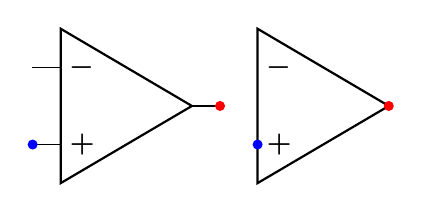
\begin{tikzpicture}[]
  \draw (0,0) node[op amp](A){};
  \ctikzset{tripoles/op amp/port width=1,
    tripoles/op amp/width=1.19, % 1.7*0.7
  }
  \draw (2.5,0) node[op amp](B){};
  \draw
    (A.out) node[red, circ]{} (A.+) node[blue, circ]{}
    (B.out) node[red, circ]{} (B.+) node[blue, circ]{};
\end{tikzpicture}
\end{LTXexample}

\paragraph{Main amplifier label.} The amplifier label (given as the text  of the node) is normally more or less centered in the shape (in the case of the triangular shape, it is shifted a bit to the left to \emph{seem} visually centered); since version \texttt{1.1.0} you can move it at the left side plus a fixed offset setting the key \texttt{component text} or the style with the same name to \texttt{left}; by default the key is \texttt{center}.
You can change the offset with the key \texttt{left text distance} (default \texttt{0.3em}; you must use a length here). These parameters are shared with IEEE-style logic ports.

\begin{LTXexample}[varwidth=true]
\begin{circuitikz}[]
    \draw (0,2.5) node[plain amp]{\texttt{741}};
    \draw (3,2.5)
        node[plain amp, component text=left]
        {\texttt{741}};
    \ctikzset{component text=left}
    \draw (0,0) node[op amp]{\texttt{741}};
    \ctikzset{left text distance=0.6em}
    \draw (3,0) node[op amp]{\texttt{741}};
\end{circuitikz}
\end{LTXexample}

These keys are also used for the positioning of the labels in the label positioning of IEEE logic gates (see~\ref{sec:ieeestdports}).

\paragraph{European-style amplifier customization.}
Thanks to the suggestions from David Rouvel (\email{david.rouvel@iphc.cnrs.fr}) there are several possible customization for the European-style amplifiers.

Since 0.9.0, the default appearance of the symbol has changed to be more in line with the standard; notice that to have a bigger triangle by default we should require more packages, and I fear {Con\TeX t} compatibility; but see later on how to change it. Notice that the font used for the symbol is defined in \texttt{tripoles/en amp/font2} and that the font used for the \texttt{+} and \texttt{-} symbols is  \texttt{tripoles/en amp/font}.

You can change the distances of the inputs, using \texttt{tripoles/en amp/input height} (default 0.3):

\begin{LTXexample}[varwidth=true]
\begin{circuitikz}
    \ctikzset{tripoles/en amp/input height=0.45}
    \draw (0,0)node[en amp](E){}
        (E.out) node[right] {$v_{\mathrm{out}}$}
        (E.-) node[left] {$v_{\mathrm{in}-}$}
        (E.+) node[left] {$v_{\mathrm{in}+}$};
\end{circuitikz}
\end{LTXexample}

and of course the key \texttt{noinv input up} is fully functional:

\begin{LTXexample}[varwidth=true]
\begin{circuitikz}
    \ctikzset{tripoles/en amp/input height=0.45}
    \draw (0,0)node[en amp, noinv input up](E){}
        (E.out) node[right] {$v_{\mathrm{out}}$}
        (E.-) node[left] {$v_{\mathrm{in}-}$}
        (E.+) node[left] {$v_{\mathrm{in}+}$};
\end{circuitikz}
\end{LTXexample}

To flip the amplifier in the horizontal direction, you can use \texttt{xscale=-1} as usual:

\begin{LTXexample}[varwidth=true]
\begin{circuitikz}
    \ctikzset{tripoles/en amp/input height=0.45}
    \draw (0,0)node[en amp, xscale=-1, noinv input up](E){}
        (E.out) node[left] {$v_{\mathrm{out}}$}
        (E.-) node[right] {$v_{\mathrm{in}-}$}
        (E.+) node[right] {$v_{\mathrm{in}+}$};
\end{circuitikz}
\end{LTXexample}

Notice that the label is fully mirrored, so check below for the generic way to change this.

You can use the new key \texttt{en amp text A} to change the infinity symbol with an A:

\begin{LTXexample}[varwidth=true]
\begin{circuitikz}
    \draw (0,0)node[en amp, en amp text A](E){}
        (E.out) node[right] {$v_{\mathrm{out}}$}
        (E.-) node[left] {$v_{\mathrm{in}-}$}
        (E.+) node[left] {$v_{\mathrm{in}+}$} ;
\end{circuitikz}
\end{LTXexample}

And if you want, you can completely change the text using the key \texttt{en amp text={}}, which by default is \verb|$\mathstrut{\triangleright}\,{\infty}$|:

\begin{LTXexample}[varwidth=true]
\begin{circuitikz}
    \draw (0,0)node[en amp, en amp text={%
            ${\triangleright}$ \small 200}](E){}
        (E.out) node[right] {$v_{\mathrm{out}}$}
        (E.-) node[left] {$v_{\mathrm{in}-}$}
        (E.+) node[left] {$v_{\mathrm{in}+}$} ;
\end{circuitikz}
\end{LTXexample}

Notice two things here: the first, that \verb|\triangleright| is enclosed in braces to remove the default spacing it has as a binary operator, and that \texttt{en amp text A} is simply a shortcut for

\begin{lstlisting}
    en amp text={$\mathstrut{\triangleright}\,\mathrm{A}$}
\end{lstlisting}


To combine flipping with a generic label you just do:

\begin{LTXexample}[varwidth=true]
\begin{circuitikz}
    \draw (0,0)node[en amp, xscale=-1, en amp text A](E){}
        (E.out) node[left] {$v_{\mathrm{out}}$}
        (E.-) node[right] {$v_{\mathrm{in}-}$}
        (E.+) node[right] {$v_{\mathrm{in}+}$} ;
\end{circuitikz}
\end{LTXexample}

But notice that the ``A'' is also flipped by the \texttt{xscale} parameter. So the solution in this case is to use \texttt{scalebox}, like this:

\begin{LTXexample}[varwidth=true]
\begin{circuitikz}
    \draw (0,0)node[en amp, xscale=-1, en amp text={%
    ${\triangleright}$ \scalebox{-1}[1]{\small 200}}](E){}
        (E.out) node[left] {$v_{\mathrm{out}}$}
        (E.-) node[right] {$v_{\mathrm{in}-}$}
        (E.+) node[right] {$v_{\mathrm{in}+}$} ;
\end{circuitikz}
\end{LTXexample}


\subsubsection{Designing your own amplifier}\label{sec:muxdemux-amplis}

If you need a different kind of amplifier, you can use the \texttt{muxdemux}
(see section~\ref{sec:muxdemuxes}) shape for defining one that suits your needs
(you need version \texttt{1.0.0} for this to work,
and \texttt{1.3.8} for the \texttt{draw only...} option).

\begin{LTXexample}[varwidth=true]
\tikzset{tdax/.style={muxdemux,
        muxdemux def={NL=2, Lh=3, NR=1, Rh=0,
        NB=4, NT=5}, font=\scriptsize\ttfamily}}
\begin{circuitikz}
    \draw (0,0) node[tdax](A){TDA1};
    \draw (2.5,0) node[tdax, muxdemux def={Rh=0.5},
    draw only top pins={1,4-5}]{TDA2};
\end{circuitikz}
\end{LTXexample}


\subsection{Switches, buttons and jumpers}

Switches and buttons come in to-style (the simple ones and the pushbuttons), and as nodes.

The switches can be scaled with the key \texttt{switches/scale} (default \texttt{1.0}). Notice that scaling the switches will not scale the poles, which are controlled with their own parameters (see section~\ref{sec:terminals}).

\subsubsection{Traditional switches}
These are all of the to-style type:

\begin{groupdesc}
    \circuitdescbip[cspst]{switch}{Switch}{spst}
    \circuitdescbip[cspst]{closing switch}{Closing switch}{cspst}
    \circuitdescbip[ospst]{opening switch}{Opening switch}{ospst}
    \circuitdescbip[nos]{normal open switch}{Normally open switch}{nos}
    \circuitdescbip[ncs]{normal closed switch}{Normally closed switch}{ncs}
    \circuitdescbip[oncs]{opening normal closed switch}{Opening normally closed switch}{oncs}
    \circuitdescbip[cncs]{closing normal closed switch}{Closing normally closed switch}{cncs}
    \circuitdescbip[onos]{opening normal open switch}{Opening normally open switch}{onos}
    \circuitdescbip[cnos]{closing normal open switch}{Closing normally open switch\footnotemark}{cnos}
    \footnotetext{These last four were contributed by \href{https://tex.stackexchange.com/questions/693446/new-switch-components-for-circuitikz}{Jakob «DraUX»}}
    \circuitdescbip[pushbutton]{push button}{Normally open push button}{normally open push button, nopb}(tip/0/0.2)
    \circuitdescbip[ncpushbutton]{normally closed push button}{Normally closed push button}{ncpb}(tip/0/0.2)
    \circuitdescbip[pushbuttonc]{normally open push button closed}{Normally open push button (in closed position)}{nopbc}(tip/0/0.2)
    \circuitdescbip[ncpushbuttono]{normally closed push button open}{Normally closed push button (in open position)}{ncpbo}(tip/0/0.2)
    \circuitdescbip[toggleswitch]{toggle switch}{Toggle switch}{}
    \circuitdescbip*{reed}{Reed switch}{}
\end{groupdesc}

while this is a node-style component:

\begin{groupdesc}
        \circuitdesc{spdt}{spdt}{}( in/180/0.2, out 1/0/0.2, out 2/0/0.2 )
\end{groupdesc}

\begin{LTXexample}[varwidth=true]
\begin{circuitikz} \draw
  (0,0) node[spdt] (Sw) {}
  (Sw.in) node[left] {in}
  (Sw.out 1) node[right] {out 1}
  (Sw.out 2) node[right] {out 2}
;\end{circuitikz}
\end{LTXexample}

\begin{LTXexample}[varwidth=true]
\begin{circuitikz} \draw
 (0,0) to[C] (1,0) to[toggle switch , n=Sw] (2.5,0)
   -- (2.5,-1) to[battery1] (1.5,-1) to[R] (0,-1) -| (0,0)
  (Sw.out 2) -| (2.5, 1) to[R] (0,1) -- (0,0)
;\end{circuitikz}
\end{LTXexample}

\subsubsection{Cute switches}
These switches have been introduced after version 0.9.0, and they come in also in to-style and in node-style, but they are size-matched so that they can be used together in a seamless way.

The path element (to-style) are:
\begin{groupdesc}
    \circuitdescbip[cuteclosedswitch]{cute closed switch}{Cute closed switch}{ccsw}(mid/90/0.2, in/-135/0.2, out/-45/0.2)
    \circuitdescbip[cuteopenswitch]{cute open switch}{Cute open switch}{cosw}(out/45/0.2)[out.s/-90/0.2]
    \circuitdescbip[cuteclosingswitch]{cute closing switch}{Cute closing switch}{ccgsw}
    \circuitdescbip[cuteopeningswitch]{cute opening switch}{Cute opening switch}{cogsw}
\end{groupdesc}
while the node-style components are the single-pole, double-throw (\texttt{spdt}) ones:
\begin{groupdesc}
    \circuitdesc{cute spdt up}{Cute spdt up}{}( in/180/0.2, out 1/0/0.2, out 2/0/0.2 , mid/0/0.4)
    \circuitdesc{cute spdt mid}{Cute spdt mid}{}
    \circuitdesc{cute spdt down}{Cute spdt down}{}(mid/0/0.4)
    \circuitdesc{cute spdt up arrow}{Cute spdt up with arrow}{}
    \circuitdesc{cute spdt mid arrow}{Cute spdt mid with arrow}{}
    \circuitdesc{cute spdt down arrow}{Cute spdt down with arrow}{}
\end{groupdesc}


\paragraph{Cute switches anchors}

The nodes-style switches have the following anchors:

\bigskip
\begin{circuitikz}
    \def\coorda(#1)<#2>{node[circle, red, draw, inner sep=1pt,pin={[red, overlay, inner sep=0.5pt, font=\small, pin distance=0.1cm, pin edge={red, overlay,}]#2:#1}](#1){}}
    \path (0,-1) -- (3,1); %bbox
    \draw (0, 0) node[spdt](S){};
    \foreach \a/\b in {center/0, in/-135, out 1/45, out 2/-45}
        \path (S.\a) \coorda(\a)<\b>;
    \draw (3, 0) node[cute spdt up arrow](CS){};
    \foreach \a/\b in {center/0, in/-135, out 1/45, out 2/-45, mid/135}
        \path (CS.\a) \coorda(\a)<\b>;
    \draw (6, 0) node[cute spdt up arrow](CS2){};
    \foreach \a/\b in {cin/-135, cout 1/45, cout 2/-45}
        \path (CS2.\a) \coorda(\a)<\b>;
\end{circuitikz}

Please notice the position of the normal anchors at the border of the \texttt{ocirc} shape for the cute switches; they are thought to be compatible with an horizontal wire going out.
Additionally, you have the \texttt{cin}, \texttt{cout 1} y \texttt{cout 2} which are anchors on the center of the contacts.

For more complex situations, the contact nodes are available\footnote{Thanks to \texttt{@marmot} on \href{https://tex.stackexchange.com/a/492599/38080}{tex.stackexchange.com}.} using the syntax \emph{name of the node}\texttt{-in}, \dots\texttt{-out 1} and \dots\texttt{-out 2}, with all their anchors.

\begin{LTXexample}[varwidth=true]
\begin{circuitikz}
\draw (0,0) node[cute spdt up] (S1) {}
  (S1.in) node[left] {in}
  (S1.out 1) node[right] {out 1};
  \draw (0,-2) node[cute spdt up,
      /tikz/circuitikz/bipoles/cuteswitch/height=0.8] (S2) {}
  (S2.in) node[left] {in}
  (S2.out 2) node[right] {out 2};
  \draw [red] (S1-in.s) -- (S2-in.n);
  \draw [blue] (S1-out 2.s) -- (S2-out 1.n);
\end{circuitikz}
\end{LTXexample}

The \texttt{mid} anchor in the cute switches (both path- and node-style) can be used to combine switches to get more complex configurations:

\begin{LTXexample}[varwidth=true]
\begin{circuitikz}
    \draw (0,1.4) node[cute spdt up](S1){};
    \draw (0,0)   node[cute spdt up](S2){};
    \draw (0,-1)  node[cuteclosedswitchshape, yscale=-1](S3){};
    \draw [densely dashed] (S1.mid)--(S2.mid)--(S3.mid);
\end{circuitikz}
\end{LTXexample}

\paragraph{Cute switches customization}

You can use the key \texttt{bipoles/cuteswitch/thickness} to decide the thickness of the switch lever.
The units are the diameter of the \texttt{ocirc} connector, and the default is \texttt{1}.

\begin{LTXexample}[varwidth=true]
\begin{circuitikz}
    \ctikzset{bipoles/cuteswitch/thickness=0.5}
    \draw (0,1.4) node[cute spdt up](S1){};
    \draw (0,0)   node[cute spdt up](S2){};
    \draw (0,-1)  node[cuteclosedswitchshape, yscale=-1](S3){};
    \draw [densely dashed] (S1.mid)--(S2.mid)--(S3.mid);
\end{circuitikz}
\end{LTXexample}

Finally, the switches are normally drawn using the \texttt{ocirc} shape, but you can change it, as in the following example, with the key \texttt{bipoles/cuteswitch/shape}. Be careful that the shape is used with its defaults (which can lead to strange results), and that the standard anchors will be correct only for \texttt{circ} and \texttt{ocirc} shapes, so you have to use the internal node syntax to connect it.

\begin{LTXexample}[varwidth=true]
\begin{circuitikz}
    \begin{scope}
        \ctikzset{bipoles/cuteswitch/thickness=0.5,
        bipoles/cuteswitch/shape=circ}
        \draw (0,2) node[cute spdt up](S1){};
        \ctikzset{bipoles/cuteswitch/thickness=0.25,
        bipoles/cuteswitch/shape=emptyshape}
        \draw (0,0) node[cute spdt up](S2){};
        \draw (S2.cin) node[draw, inner sep=2pt]{};
        \draw (S2.cout 1) node[draw, inner sep=2pt]{};
        \draw (S2.cout 2) node[draw=red, inner sep=2pt]{};
    \end{scope}
    \draw (0,-2)  node[cuteclosedswitchshape, yscale=-1](S3){};
    \draw [densely dashed] (S1.mid)--(S2.mid)--(S3.mid);
\end{circuitikz}
\end{LTXexample}

\subsubsection{Proximity switches}

\begin{groupdesc}
    \circuitdesc*{proximeter}{proximeter}{text}(hlines nw/135/0.4, hlines ne/45/0.4, hlines sw/-135/0.4, hlines se/-45/0.4, center/-90/0.4)
    \circuitdescbip*{inline proximeter}<proximeter>{proximeter switch, inline}{}(left/135/0.4, right/45/0.4)
\end{groupdesc}

The \texttt{proximeter} shape\footnote{Suggested by \href{https://github.com/circuitikz/circuitikz/issues/631}{Anisio Rogerio Braga}, implemented in \texttt{v1.5.2}; see also \href{https://knowledge.autodesk.com/support/autocad-electrical/learn-explore/caas/CloudHelp/cloudhelp/2019/ENU/AutoCAD-Electrical/files/GUID-1B18023D-241C-4E50-822A-94F873FC258B-htm.html}{here}.} can be used as a dipole with the \texttt{inline proximeter} variant.

It has been assigned to the \texttt{switches} class; you can adjust the (relative) thickness of the inside horizontal lines with the key \texttt{proximeter/hlines thickness} (default \texttt{0.5}) and their vertical position with \texttt{proximeter/hlines position} (default \texttt{0.3}). You can also change the default size of \emph{all} proximeter symbols by changing \texttt{proximeter/width} (only safe at picture level; better set in the preamble if you need to change it. The default value is \texttt{0.3}).

Notice in the following example that, as ever for node-type shape, the text is not included in the bounding box:
\begin{LTXexample}[varwidth=true, basicstyle=\small\ttfamily]
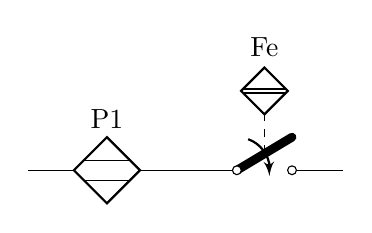
\begin{tikzpicture}
    \tikzset{small up proxi/.style={proximeter, solid,
            circuitikz/switches/scale=0.707,
            circuitikz/proximeter/hlines thickness=1,
            circuitikz/proximeter/hlines position=0.1}}
    \draw (0,0) to[inline proximeter, l=P1] ++(2,0)
        to[ccgsw, name=P2] ++(2,0);
    \draw[dashed] (P2.mid) -- ++(0,0.5)
        node[small up proxi, above](P2p){Fe}
        (P2p.north) ++ (0,0.5); % extend bounding box
\end{tikzpicture}
\end{LTXexample}

\subsubsection{Rotary switches}

Rotary switches are a kind of generic multipole switches; they are implemented as a strongly customizable element (and a couple of styles to simplify its usage). The basic element is the following one, and it has the same basic anchors of the cute switches, included the access to internal nodes (shown in blue here).

\begin{groupdesc}
\circuitdesc{rotaryswitch}{Rotary switch}{}(in/-180/0.2, cin/145/0.2, center/-90/0.2, mid/0/0.4, out 1/0/0.2,
cout 1/180/0.2)[out 1.n/90/0.2, out 4.w/0/0.3]
\end{groupdesc}

Notice that the name of the shape is \texttt{rotaryswitch}, no spaces.
The default rotary switch component has 5 channels (this is set in the parameter \texttt{multipoles/rotary/channels}), spanning form \SI{-60}{\degree}  to \SI{60}{\degree} (parameter \texttt{multipoles/rotary/angle}) and with the wiper at \SI{20}{\degree} (parameter \texttt{multipoles/rotary/wiper}).

Moreover, there are by default no arrows on the wiper; if needed, you can change this default setting the parameter \texttt{multipoles/rotary/arrow} which can assume the values \texttt{none}, \texttt{cw} (clockwise), \texttt{ccw} (counterclockwise) or \texttt{both}.

To simplify the usage of the component, a series of styles are defined: \texttt{rotary switch=\textsl{<channels>} in \textsl{<angle>} wiper \textsl{<wiper angle>}} (notice the space in the name of the style!). Using \texttt{rotary switch} without parameters will generate a default switch.

To add arrows, you can use the styles \texttt{rotary switch -} (no arrow, whatever the default), \texttt{rotary switch <-} (counterclockwise arrow), \texttt{rotary switch ->} (clockwise) and \texttt{rotary switch <->} (both).

Notice that the defaults of the styles are the same as the default values of the parameters, but that if you change globally the defaults using the keys mentioned above, you only change the defaults for the ``bare'' component \texttt{rotaryswitch}, not for the styles.


\begin{LTXexample}[varwidth=true, pos=t]
\begin{circuitikz}
\ctikzset{multipoles/rotary/arrow=both}
\draw (0,0) -- ++(1,0) node[rotary switch <-=8 in 120 wiper 40, anchor=in](A){};
\draw (3,0) -- ++(1,0) node[rotary switch, anchor=in](B){}; % default values
\draw[red] (A.out 4) -| (3,0);
\draw[blue] (A-out 2.n) -- ++(0,0.5) -| (B-out 1.n);
\draw (B.out 3) -- ++(1,0) node[rotary switch -=5 in 90 wiper 15, anchor=in](C){};
\draw (C.out 3) -- ++(1,0) node[rotary switch ->, xscale=-1, anchor=out 3](D){};
\draw[green, dashed] (B.mid) -- ++(-.5,-1) -| (C.mid);
\end{circuitikz}
\end{LTXexample}

\paragraph{Rotary switch anchors}

Rotary switches anchors are basically the same as the cute switches, including access (with the \texttt{\textsl{<node name>}-<anchor name>} notation) to the internal connection nodes. The geographical anchors work as expected, marking the limits of the component.

\showanchors{rotary switch}{}(north/90/0.4, north east/45/0.4, east/0/0.4, south east/-45/0.4,
    south/-90/0.4, south west/-135/0.4, west/180/0.4, north west/135/0.4, center/-120/0.3)
\qquad
\showanchors{rotary switch=25 in 120 wiper 10}{}(north/90/0.4, north east/45/0.4, east/0/0.4, south east/-45/0.4,
    south/-90/0.4, south west/-135/0.4, west/180/0.4, north west/135/0.4, center/-120/0.3)

In addition to the anchors they have in common with the cute switches, the rotary switch has the so called ``angled'' anchors and the ``external square anchors''. \emph{Angled anchors}, called \texttt{aout 1}, \texttt{aout 2} and so forth, are anchors placed on the output poles at the same angle as the imaginary lines coming from the input pole; \emph{square anchors}, called \texttt{sqout 1}\dots,  are located on an imaginary square surrounding the rotary switch on the same line.

\bigskip

\begin{circuitikz}
    \begin{scope}[scale=2, transform shape]
        \clip (-1,-.4) rectangle (1,.6);
        \draw (0,0) node[rotary switch=9 in 90 wiper 10](Z){};
        \draw [dashed, blue] (Z.cin) -- (Z.sqout 4);
    \end{scope}
    \path (Z.aout 4) \showcoord(aout 4)<-15:0.4>;
    \path (Z.sqout 4) \showcoord(sqout 4)<0:0.4>;
    \path (Z.out 3) \showcoord(out 3)<15:0.4>;
    \path (Z.cout 3) \showcoord(cout 3)<180:0.4>;
    \draw (8,0) node[rotary switch -=31 in 150 wiper 10](D){};
    \foreach \i in {1,...,31} \draw (D.sqout \i) -- (D.aout \i);
    \foreach \l/\a/\d in {north/90/0.2, north east/45/0.2, east/0/0.2,
        south east/-45/0.2, south/-90/0.2, south west/-135/0.2, west/180/0.2, north west/135/0.2,
    center/-145/0.7}
    \path (D.ext \l) \showcoord(ext \l)<\a:\d>;
    \path (D.aout 12)  \showcoordb(aout 12)<-5:0.4>;
    \path (D.sqout 12)  \showcoordb(sqout 12)<0:0.4>;
    \draw[blue, densely dotted] (D.ext north west) rectangle (D.ext south east);
\end{circuitikz}

The code for the diagram at the left, above, without the markings for the anchors, is:
\begin{lstlisting}[basicstyle=\small\ttfamily]
\begin{circuitikz}
    \draw (8,0) node[rotary switch -=31 in 150 wiper 10](D){};
    \foreach \i in {1,...,31} \draw (D.sqout \i) -- (D.aout \i);
    \draw[blue, densely dotted] (D.ext north west) rectangle (D.ext south east);
\end{circuitikz}
\end{lstlisting}

One possible application for the angled and the ``on square'' anchors is that you can use them to move radially from the output poles, for example for adding numbers:

\begin{LTXexample}[varwidth=true]
\begin{circuitikz}
\draw (0,0) node[rotary switch=13 in 120 wiper 0](S){};
\foreach \i in {1,...,13} % requires "calc"
    \path ($(S.aout \i)!1ex!(S.sqout \i)$)
        node[font=\tiny\color{red}]{\i};
\end{circuitikz}
\end{LTXexample}

Finally, notice that the value of width for the rotary switches is taken from the one for the ``cute switches'' which in turn is taken from the width of traditional  \texttt{spdt} switch, so that they match (notice that the ``center'' anchor is better centered in the rotary switch, so you have to explicitly align them).

\begin{LTXexample}[varwidth=true]
\begin{circuitikz}
    \draw (0,0) node[color=blue, rotary switch=2 in 35 wiper 30,
        anchor=in](R){};
    \draw (0,-1) node[cute spdt up, anchor=in](C){};
    \draw (0,-2) node[color=blue, rotary switch=3 in 35 wiper 30,
        anchor=in](R){};
\end{circuitikz}
\end{LTXexample}

\paragraph{Rotary switch customization}

Apart from the basic customization seen above (number of channels, etc.) you can change, as in the cute switches, the shape used by the connection points with the parameter \texttt{multipoles/rotary/shape}, and the thickness of the wiper with \texttt{multipoles/rotary/thickness}. The optional arrow has thickness equal to the standard bipole thickness \texttt{bipoles/thickness} (default 2).

\begin{LTXexample}[varwidth=true]
\begin{circuitikz}
    \ctikzset{multipoles/rotary/thickness=0.5}
    \draw (0,1.6) node[rotary switch ->, color=blue](S1){};
    \ctikzset{multipoles/rotary/shape=circ}
    \draw (0,0) node[rotary switch ->](S2){};
    \ctikzset{bipoles/thickness=0.5}
    \draw (0,-1.6) node[rotary switch ->, color=red](S3){};
\end{circuitikz}
\end{LTXexample}

Finally, the size can be changed using the parameter \texttt{tripoles/spdt/width} (default 0.85).

\begin{LTXexample}[varwidth=true]
\begin{circuitikz}
    \draw (0,2) node[rotary switch ->, color=blue](S1){};
    \ctikzset{tripoles/spdt/width=1.6, fill=cyan,
        multipoles/rotary/shape=osquarepole}
    \draw (0,0) node[rotary switch ->](S2){};
\end{circuitikz}
\end{LTXexample}

\subsubsection{Switch arrows\label{sec:switcharrows}}

You can change the arrow tips used in all switches (traditional and ``cute'') with the key \texttt{switch end arrow} (by default the key is the word ``\texttt{default}'' to obtain the default arrow, which is \texttt{latexslim}).
Also you can change the start arrow with the corresponding \texttt{switchable start arrow} or \texttt{wiper start arrow} (the default value ``\texttt{default}'' is equivalent to \texttt{\{\}}, which means no arrow). The keys are settable with \verb|\ctikzset| as with \verb|\tikzset| (to ease their usage in nodes).

You can change that globally or locally, as ever. The tip specification is the one you can find in the \TikZ{} manual (``Arrow Tip Specifications'').

\begin{LTXexample}[varwidth=true]
\begin{circuitikz}
    \draw (0,2) to[cspst] ++(2,0)
        node[cute spdt up arrow, anchor=in]{};
    \draw (0,0) to[cspst] ++(2,0)
        node[cute spdt up arrow, anchor=in,
        switch start arrow={Bar[red]},
        switch end arrow={Triangle[blue]}]{};
\end{circuitikz}
\end{LTXexample}

You can also have the option to change the color, relative thickness, and dash pattern  by setting keys with the \verb!\ctikzset! command under the \texttt{switch arrows} hierarchy. The available keys are:

\begin{center}
    \begin{tabular}{>{\ttfamily}l>{\ttfamily}lp{0.5\linewidth}}
        \toprule
     parameter &  default & description  \\
     \midrule
     relative thickness & 1.0 & multiply the class thickness \\
     color & default & stroke color: \texttt{default} is the same as the component \\
     dash & default & dash pattern: \texttt{default} means not to change the setting for the component; \texttt{none} means unbroken line; every other input is a dash pattern.\footnotemark \\
        \bottomrule
    \end{tabular}
    \footnotetext{Follows the syntax of the pattern sequence \texttt{\textbackslash pgfsetdash} --- see \TikZ{} manual for details; phase is always zero. Basically you pass pairs of dash-length -- blank-length dimensions, see the examples.}
\end{center}

\begin{LTXexample}[varwidth=true, basicstyle=\small\ttfamily]
\begin{circuitikz}
\draw (0,2) to[spst] ++(1,0) to[cogsw]
    ++(1,0) to[oncs] ++(1,0);
\ctikzset{switch arrows/color=red}
\ctikzset{switch arrows/relative thickness=0.5}
\ctikzset{switch arrows/dash={{1pt}{1pt}}}
\draw (0,0) to[spst] ++(1,0) to[cogsw, switch arrows/dash=none]
    ++(1,0) to[oncs, switch arrows/color=blue] ++(1,0);
\end{circuitikz}
\end{LTXexample}

\paragraph{Rotary switch arrows.} You can change the rotary switch arrow shape in the same way as you change the ones in regular switches. Notice however that if you set either \texttt{switch end arrow} or \texttt{switch start arrow} they will be followed only if you have set both arrows with \texttt{<->} or equivalent, otherwise just one will be used.

\begin{LTXexample}[varwidth=true, pos=t]
\begin{circuitikz}
\ctikzset{multipoles/rotary/arrow=both}
\draw (0,0) -- ++(1,0) node[rotary switch <-=8 in 120 wiper 40, anchor=in](A){};
\draw (3,0) -- ++(1,0) node[rotary switch, anchor=in](B){}; % default values
\draw (B.out 3) -- ++(1,0) node[rotary switch -=5 in 90 wiper 15, anchor=in](C){};
\draw (C.out 3) -- ++(1,0) node[rotary switch ->, xscale=-1, anchor=out 3](D){};
\ctikzset{switch end arrow={Triangle[blue]}}
\ctikzset{switch start arrow={Bar[red]}}
\begin{scope}[yshift=-2cm]
    \draw (0,0) -- ++(1,0) node[rotary switch <-=8 in 120 wiper 40, anchor=in](A){};
    \draw (3,0) -- ++(1,0) node[rotary switch, anchor=in](B){}; % default values
    \draw (B.out 3) -- ++(1,0) node[rotary switch -=5 in 90 wiper 15, anchor=in](C){};
    \draw (C.out 3) -- ++(1,0) node[rotary switch ->, xscale=-1, anchor=out 3](D){};
\end{scope}
\end{circuitikz}
\end{LTXexample}

\subsubsection{Jumpers}

You can think of jumpers like a kind of switches (they have the same function, just the way of operating them is different).
\Circuitikz{} has two types of jumper symbols available, the simple ones and the three pins (or two-ways) ones.

\paragraph{Simple jumpers.} These are the most common ones. They come in three variations, bare, open and closed.

\begin{groupdesc}
    \circuitdescbip*[bjumper]{bare jumper}{Bare jumper}{}(in/135/0.6, out/45/0.6)[out.n/90/0.2]
    \circuitdescbip*[ojumper]{open jumper}{Open jumper}{}(in/135/0.6, out/45/0.6, top arc/90/0.3)[out.s/-90/0.2]
    \circuitdescbip*[cjumper]{closed jumper}{Closed jumper}{}(left/135/0.6, right/45/0.6, top arc/90/0.3)[in.s/-90/0.2]
\end{groupdesc}

The \texttt{top arc} anchor can be used to locate the position of the top of the wire (when present). In bare jumper, the anchor is located in the middle of the connectors gap.

\begin{LTXexample}[varwidth=true, basicstyle=\small\ttfamily]
\begin{circuitikz}[scale=0.8]
    \draw (0,0) to[open jumper, l=J1] ++(2,0)
        to[closed jumper, l_=J2, name=J2] ++(2,0)
        to[bare jumper=J3] ++(2,0);
    \draw [dashed] (J2.top arc) -- ++(0,0.5)
        node[above] {\tiny open to enable};
\end{circuitikz}
\end{LTXexample}

Similarly to switches, you have access to the subnodes representing the contacts, to be able to draw wires at different angles.

The kind of poles used in the diagram can be changed with the \verb!\ctikzset! key \texttt{bipoles/jumpers/shape}.

\begin{LTXexample}[varwidth=true, basicstyle=\small\ttfamily]
\begin{circuitikz}[scale=0.8]
    \draw (0,0) to[open jumper, l=J1, name=J1] ++(2,0)
        to[closed jumper, l_=J2, name=J2,
            bipoles/jumper/shape=odiamondpole] ++(2,0);
        \draw [red] (J2-in.-135) -- ++(-135:1)
            node[font=\tiny, below]{marked \emph{hot}};
\end{circuitikz}
\end{LTXexample}

\paragraph{Two-ways (three-pins) jumpers.} In this case, the symbol represent two-ways jumpers (normally, three pins that can be connected in a couple of ways).

To maintain flexibility, every possible combination of bare, open or closed is available; but to avoid having to define too much different bipoles, a different approach is used here. You have to specify the style using a different key, namely \texttt{tjumper connections}.

\begin{groupdesc}
    \circuitdescbip*[tjumper]{three-pins jumper}{Three-pins jumper (see later for connections)}{}(in/135/0.6, out/45/0.6, tap/-90/0.2)[out.n/90/0.2]
    \ctikzset{tjumper connections=12}
    \circuitdescbip*[tjumper]{three-pins jumper}{Three-pins jumper (connections \texttt{\ctikzvalof{tjumper connections}})}{}(top arc left/135/0.6, top arc right/45/0.6, tap/-145/0.2)[out.n/-90/0.2]
    \ctikzset{tjumper connections=S1}
    \circuitdescbip*[tjumper]{three-pins jumper}{Three-pins jumper (connections \texttt{\ctikzvalof{tjumper connections}})}{}(top arc left/135/0.6, top arc right/45/0.6, tap/-145/0.2)[out.n/-90/0.2]
\end{groupdesc}

The option is used as shown in the following example, or by setting the key using \verb!\ctikzset!. The value \textbf{must} be two characters, either two numbers (where \texttt{0} means ``bare'', \texttt{1} means ``open'', and \texttt{2} means ``closed'') or the letter \texttt{S} (for ``span'') and one number. In the latter case, the arc will connect the fist and last pole\footnote{Although really I never saw an example of this use\dots You never know.}

\begin{LTXexample}[varwidth=true, pos=t, basicstyle=\small\ttfamily]
\begin{circuitikz}
    \draw (0,1.5) to[three-pins jumper, l=J1, name=T] ++(3,0)
    to[three-pins jumper, tjumper connections=21, l=J2] ++(3,0)
    to[three-pins jumper, tjumper connections=20, l=J3] ++(3,0);
    \draw (T.tap) -- ++(0,-0.5);
    \ctikzset{bipoles/jumper/shape=osquarepole}
    \draw (0,0) to[three-pins jumper, l=JA, name=T] ++(3,0)
    to[three-pins jumper, tjumper connections=S1, l=JB] ++(3,0)
    to[three-pins jumper, tjumper connections=S2, l=JB] ++(3,0);
\end{circuitikz}
\end{LTXexample}

\subsubsection{Solder jumpers.} Solder jumpers are basically jumpers that can be closed or opened on the printed circuit board. Although electrically they behave exactly as jumpers, these are thought to change configurations in a more stable way (to change them from their default connection you have to use a cutter and/or a soldering iron).

\begin{groupdesc}
    \circuitdescbip[osjumper]{open solder jumper}{Open solder jumper}{}(in/135/0.3, out/45/0.3)
    \circuitdescbip[csjumper]{closed solder jumper}{Closed solder jumper}{}(left/135/0.3, right/45/0.3)
    \circuitdescbip[odsjumper]{open double solder jumper}{Open double solder jumper}{}(in/135/0.3, out/45/0.3, tap/90/0.1)
    \circuitdescbip[ldsjumper]{left double solder jumper}{Left double solder jumper}{}(left/135/0.3, right/45/0.3,
        tap up/90/0.1, tap down/-90/0.1)
    \circuitdescbip[rdsjumper]{right double solder jumper}{Right double solder jumper}{}(left/135/0.3, right/45/0.3,
        tap up/90/0.1, tap down/-90/0.1)
    \circuitdescbip[cdsjumper]{closed double solder jumper}{Closed double solder jumper}{}
\end{groupdesc}

\begin{LTXexample}[varwidth=true, basicstyle=\small\ttfamily]
\begin{circuitikz}[scale=0.8]
    \draw (0,0) to[open solder jumper, l=J1] ++(2,0)
        to[closed solder jumper, l_=J2, name=J2] ++(2,0)
        to[right double solder jumper, l=J3,
            name=J3] ++(2,0);
    \draw (J3.tap down) -- ++(0,-1) node[ocirc]{};
\end{circuitikz}
\end{LTXexample}


\subsection{Logic gates}

Logic gates, with two or more input, are supported. Albeit in principle these components are multipoles, the are considered tripoles here, for historical reasons (when they just had two inputs).

\subsubsection{American Logic gates}
\begin{groupdesc}
    \circuitdesc*{american and port}{American \textsc{and} port}{}( in 1/180/0.2, in 2/180/0.2, out/0/0.2 )
    \circuitdesc*{american or port}{American \textsc{or} port}{}( bin 1/135/0.2, bin 2/-135/0.2, bout/-45/0.2 )
    \circuitdesc*{american nand port}{American \textsc{nand} port}{}
    \circuitdesc*{american nor port}{American \textsc{nor} port}{}
    \circuitdesc*{american xor port}{American \textsc{xor} port}{}
    \circuitdesc*{american xnor port}{American \textsc{xnor} port}{}
    \circuitdesc*{american buffer port}{American \textsc{buffer} port}{}
    \circuitdesc*{american not port}{American \textsc{not} port}{}
\end{groupdesc}

There is no ``european''  version of the following symbols; for now they are used both in \texttt{american} and \texttt{european} styles, but iy may change in the future.

\begin{groupdesc}
    \circuitdesc*{schmitt}{Non-Inverting Schmitt trigger}{}
    \circuitdesc*{invschmitt}{Inverting Schmitt trigger}{}
\end{groupdesc}

\subsubsection{IEEE logic gates}\label{sec:ieeestdports}

In addition to the legacy ports, since release 1.1.0, logic ports following the recommended geometry of distinctive-shape symbols in IEEE Std 91a-1991 Annex A (Recommended symbol proportions) are also available\footnote{Thanks to Jason for proposing it and digging out the info, see this \href{https://github.com/circuitikz/circuitikz/issues/383}{GitHub issue}.}.

These ports are completely independent from the legacy set (either \texttt{american} or \texttt{european}); they are not enabled by default because the relative size of the ports is very different from the legacy ones, and that will disrupt every schematic (especially if drawn with absolute coordinate). If you want to use them as default, you can use the command \verb|\ctikzset{logic ports=ieee}| and by default the shapes \texttt{and port}, \texttt{or port} and so on will be the IEEE standard ones.

The transmission gate (also known as ``bowtie'') components are not described in the IEEE standard, so they are simply inspired by the other IEEE ports --- this is why their name is prefixed by \texttt{ieee} and not by \texttt{ieeestd}. They are aliased to \texttt{tgate} and \texttt{double tgate} though, and it is recommended to use those names (maybe in the future there will be \texttt{american ports} and/or \texttt{european ports} versions available).

\begin{groupdesc}
    \circuitdesc*{ieeestd and port}{IEEE standard ``and'' port}{}(in 1/180/0.2, in 2/180/0.2, out/0/0.2, bout/45/0.2)
    \circuitdesc*{ieeestd nand port}{IEEE standard ``nand'' port}{}(in 1/180/0.2, out/0/0.2, bout/45/0.2)
    \circuitdesc*{ieeestd or port}{IEEE standard ``or'' port}{}(in 1/180/0.2, bin 2/-155/0.2, out/0/0.2, bout/45/0.2)
    \circuitdesc*{ieeestd nor port}{IEEE standard ``nor'' port}{}(left/180/0.2, center/-45/0.4, up/30/0.2,
        down/-30/0.2)[not/45/0.3]
    \circuitdesc*{ieeestd xor port}{IEEE standard ``xor'' port xor}{}(left/180/0.2, bin 1/145/0.3, ibin 1/45/0.3, right/45/0.2)
    \circuitdesc*{ieeestd xnor port}{IEEE standard ``xnor'' port}{}(body left/70/0.4, body right/-70/0.3,
        out/0/0.2, bout/45/0.2)
    \circuitdesc*{ieeestd buffer port}{IEEE standard buffer port}{}(in 1/180/0.2, bin 1/-155/0.2, up/30/0.2, down/-30/0.2)
    \circuitdesc*{ieeestd not port}{IEEE standard ``not'' port}{}(in/180/0.2, bin/-155/0.2, out/0/0.2, bout/45/0.2)
    \circuitdesc*{ieeestd schmitt port}{Schmitt port matched to IEEE standard ports}{}(in/180/0.2, out/0/0.2, bout/45/0.2)
    \circuitdesc*{ieeestd invschmitt port}{Inverting Schmitt port matched to IEEE standard ports}{}
    \circuitdesc*{ieee tgate}{IEEE style transmission gate}{}(in 1/180/0.2, bin 1/-155/0.2, up/30/0.2, down/-30/0.2, out/0/0.2, bout/45/0.2, notgate/135/0.4, gate/-135/0.4)
    \circuitdesc*{ieee double tgate}{IEEE style double transmission gate}{}(in/180/0.2, bin/-155/0.2, out/0/0.2, bout/45/0.2, up/30/0.2, down/-30/0.2, bnotgate/135/0.4, bgate/-115/0.4)
    \circuitdesc*{notcirc}{Inverting dot for IEEE ports}{}(west/180/0.1, east/0/0.1)
    \circuitdesc*{schmitt symbol}{Schmitt symbol to add to input pins if needed}{}(north west/145/0.1, south east/-45/0.1)

\end{groupdesc}

\subsubsection{European Logic gates}
\begin{groupdesc}
    \circuitdesc*{european and port}{European \textsc{and} port}{}( in 1/180/0.2, in 2/180/0.2, out/0/0.2 )
    \circuitdesc*{european or port}{European \textsc{or} port}{}( bin 1/135/0.2, bin 2/-135/0.2, bout/-45/0.2 )
    \circuitdesc*{european nand port}{European \textsc{nand} port}{}
    \circuitdesc*{european nor port}{European \textsc{nor} port}{}
    \circuitdesc*{european xor port}{European \textsc{xor} port}{}
    \circuitdesc*{european xnor port}{European \textsc{xnor} port}{}
    \circuitdesc*{european buffer port}{European \textsc{buffer} port}{}
    \circuitdesc*{european not port}{European \textsc{not} port}{}
    \circuitdesc*{european blank port}{European blank port}{A}
    \circuitdesc*{european blank not port}{European blank not port}{B}
\end{groupdesc}

\begin{framed}
If (default behaviour) \texttt{americanports} option is active (or the style \texttt{[american ports]} is used), the shorthands \texttt{and port}, \texttt{or port}, \texttt{buffer port}, \texttt{nand port}, \texttt{nor port},  \texttt{not port}, \texttt{xor port}, \texttt{xnor port}, \texttt{schmitt port} and \texttt{invschmitt port}  are equivalent to the american version of the respective logic port.

If otherwise \texttt{europeanports} option is active (or the style \texttt{[european ports]} is used), the shorthands \texttt{and port}, \texttt{or port}, \texttt{buffer port}, \texttt{nand port}, \texttt{nor port},  \texttt{not port}, \texttt{xor port}, \texttt{xnor port} are equivalent to the european version of the respective logic port; \texttt{schmitt port} and \texttt{invschmitt port} are the same as in \texttt{american ports} style.

Finally, for version \texttt{1.1.0} and up, you can use the style \texttt{ieee ports} to set the shorthands to the set of \texttt{ieeestd} ports. (There is no global option for this).
\end{framed}

\subsubsection{Path-style logic ports}

The one-input, one-output ports have a handy path-style equivalent; they are the following:

\begin{groupdesc}
    \ctikzset{logic ports=ieee}
    \circuitdescbip*{inline not}<not port>{``not''  logic port}{}
    \circuitdescbip*{inline buffer}<buffer port>{``buffer''  logic port}{}
    \circuitdescbip*{inline schmitt}<schmitt port>{Schmitt logic port}{}
    \circuitdescbip*{inline invschmitt}<invschmitt port>{Inverting Schmitt logic port}{}
    \circuitdescbip*{inline tgate}<tgate>{transmission gate}{}(bgate/-90/0.2, bnotgate/90/0.2)
    \circuitdescbip*{inline double tgate}<double tgate>{double transmission gate}{}(bgate/-90/0.2, bnotgate/90/0.2)
\end{groupdesc}

Those ports follow the current selected style, although you can change it on the fly (even if it does not have a lot of sense); you can apply labels, annotations and (again, not a lot of sense) voltages to them. The assigned value is typeset as if it were the main text of the node.

\begin{LTXexample}[varwidth=true]
\begin{circuitikz}[american]
    \ctikzset{logic ports=ieee}
    \draw (0,0) to[inline not=I1, l=label, v=$\Delta V$] ++(2,0);
    \draw (0,-2) to[inline not, a=ann, european ports] ++(2,0);
\end{circuitikz}
\end{LTXexample}

Notice that in the inline version the leading pins are not drawn,
so in the case of the transmission gates
you have to use the border pins to connect the gates.

\begin{LTXexample}[varwidth=true]
\begin{circuitikz}[ ]
    \ctikzset{logic ports=ieee,
    logic ports/fill=yellow}
    \draw (0,0) to[inline not] ++(2,0)
    to[inline double tgate, name=P] ++(3,0)
    (P.bnotgate) |- ++(-3,1);
\end{circuitikz}
\end{LTXexample}

\subsubsection{American ports usage}

Since version \texttt{1.0.0}, the default shape of the family of american ``or'' ports has changed to a more ``pointy'' one, for better distinguish them from the ``and''-type ports. You can still go back to the previous aspect with the key \texttt{american or shape} that can be set to \texttt{pointy} or \texttt{roundy}. The \texttt{legacy} style will enact the old, roundy style also.

\begin{LTXexample}[varwidth=true]
\begin{circuitikz}[
    american]
    % legacy shapes
    \ctikzset{american or shape=roundy}
    \ctikzset{logic ports/fill=yellow}
    \node [or port](O1) at (0,0) {};
    \node [nor port](O2) at (0,-1.5) {};
    \node [xor port](O3) at (0,-3) {};
    \node [xnor port](O4) at (0,-4.5) {};
    \begin{scope}[xshift=3cm]
    % new shapes
        \ctikzset{american or shape=pointy}
        \node [or port](O1) at (0,0) {};
        \node [nor port](O2) at (0,-1.5) {};
        \node [xor port](O3) at (0,-3) {};
        \node [xnor port](O4) at (0,-4.5) {};
    \end{scope}
\end{circuitikz}
\end{LTXexample}

\paragraph{American logic port customization}

Logic port class is called \texttt{logic ports}, so you can scale them all with \texttt{logic ports/scale} (default \texttt{1.0}).

As for most components, you can change the width and height of the ports; the thickness is given by the parameter \texttt{tripoles/thickness} (default 2).

It is possible to change height and width of the logic ports using the parameters \texttt{tripoles/american \emph{type} port/} plus \texttt{width} or \texttt{height}:

\begin{LTXexample}[varwidth=true]
\tikz \draw (0,0) node[nand port] {}; \par
\ctikzset{tripoles/american nand port/input height=.2}
\ctikzset{tripoles/american nand port/port width=.4}
\ctikzset{tripoles/thickness=4}
\tikz \draw (0,0) node[nand port] {};
\end{LTXexample}


This is especially useful if you have ports with more than two inputs, which are instantiated
with the parameter \texttt{number inputs} :

\begin{LTXexample}[varwidth=true]
\begin{circuitikz}
\draw (0,3) node[american and port] (A)  {P1};
\begin{scope}
    \ctikzset{tripoles/american or port/height=1.6}
    \draw (A.out) -- ++(0.5,0)
    node[american or port,
    number inputs=5,
    anchor=in 1] (B)  {P2};
\end{scope}
\draw (0,1.5) node[american or port] (C)  {P3};
\draw (C.out) |- (B.in 2);
\end{circuitikz}
\end{LTXexample}

You can suppress the drawing of the logic ports input leads by using the boolean key \texttt{logic ports draw input leads}  (default \texttt{true}) or, locally, with the style \texttt{no inputs leads} (that can be reverted with \texttt{input leads}),  like in the following example. The anchors do not change and you have to take responsibility to make the connection to the ``border''-anchors.

\begin{LTXexample}[varwidth=true]
\begin{circuitikz}
    \node [or port](O1) at (0,2) {};
    \node [or port, no input leads](O1) at (2,2) {};
    \ctikzset{logic ports draw input leads=false}
    \node [and port](O1) at (0,0) {};
    \node [nand port, input leads](O1) at (2,0) {};
\end{circuitikz}
\end{LTXexample}

This is useful if you need to draw a generic port, like the one following here:

\begin{LTXexample}[varwidth=true]
\begin{circuitikz}
    \ctikzset{tripoles/american nand port/height=1.6}
    \draw (0,0)
    node[american nand port,
    circuitikz/tripoles/american nand port/height=1.1,
    number inputs=5, no input leads,
    ] (B) {Pn};
    \draw (B.in 1) -- (B.bin 1) (B.in 5) -- (B.bin 5);
    \node[rotate=90] at (B.in 3) {\dots};
\end{circuitikz}
\end{LTXexample}

In an analogous manner, there is a setting \texttt{logic ports draw output leads} (and a corresponding style \texttt{no output leads}) that suppresses the drawing of the output lead. A shortcut boolean key \texttt{logic ports draw leads} will suppress or enable all leads (the corresponding styles are \texttt{no leads} and \texttt{all leads}).

You can tweak the appearance of american ``or'' family (\texttt{or}, \texttt{nor}, \texttt{xor}  and \texttt{xnor}) ports, too, with the parameters \texttt{inner} (how much the base circle goes ``into'' the shape, default 0.3) and \texttt{angle} (the angle at which the base starts, default 70).

\begin{LTXexample}[varwidth=true]
\tikz \draw (0,0) node[xnor port] {};
\ctikzset{tripoles/american xnor port/inner=.7}
\ctikzset{tripoles/american xnor port/angle=40}
\tikz \draw (0,0) node[xnor port] {};
\end{LTXexample}

\paragraph{American logic port anchors}

These are the anchors for logic ports:

\bigskip
\begin{circuitikz} [american]
\def\coorda(#1)<#2>{node[circle, red, draw, inner sep=1pt,pin={[red, overlay, inner sep=0.5pt, font=\small, pin distance=0.1cm, pin edge={red, overlay,}]#2:#1}](#1){}}
\path(-2,1) -- (11,-1);

\draw (0,0) node[and port, number inputs=3](A){IC1} ;
  \foreach \a/\d in {left/45, right/45, out/-45, in 1/135, in 2/135, in 3/135}
    \path (A.\a) \coorda(\a)<\d>;

\draw (4.5,0) node[and port, number inputs=3](A){IC1};
  \foreach \a/\d in {north/90, north west/135, west/180, south west/-135,
  south/-90, south east/45, east/45, north east/45}
    \path (A.\a) \coorda(\a)<\d>;

\draw (9,0) node[nand port, ](A){} ;
  \foreach \a/\d in {left/45, right/45, center/-90}
    \path (A.\a) \coorda(\a)<\d>;
\end{circuitikz}
\bigskip

You also have ``border pin anchors'':

\bigskip
\begin{circuitikz} [american]
\def\coorda(#1)<#2>{node[circle, red, draw, inner sep=1pt,pin={[red, overlay, inner sep=0.5pt, font=\small, pin distance=0.1cm, pin edge={red, overlay,}]#2:#1}](#1){}}
\path(-2,1) -- (11,-1);

\draw (0,0) node[american and port, number inputs=3](A){IC1} ;
  \foreach \a/\d in {bin 1/-135, bin 2/-135, bin 3/-135, bout/-45}
    \path (A.\a) \coorda(\a)<\d>;

\draw (4.5,0) node[american or port, number inputs=3](A){IC1};
  \foreach \a/\d in {bin 1/-135, bin 2/-135, bin 3/-135, bout/-45}
    \path (A.\a) \coorda(\a)<\d>;

\draw (9,0) node[nand port, ](A){} ;
  \foreach \a/\d in {bin 1/-135, bin 2/-135, bout/-45}
    \path (A.\a) \coorda(\a)<\d>;
\end{circuitikz}
\bigskip

These anchors are especially useful if you want to negate inputs:

\begin{LTXexample}[varwidth=true]
\begin{circuitikz}
\draw (0,3) node[american and port] (A)  {P1};
\node at (A.bin 1) [ocirc, left]{} ;
\begin{scope}
    \ctikzset{tripoles/american or port/height=1.6}
    \draw (A.out) -- ++(0.5,0) node[american or port,
    number inputs=5, anchor=in 1] (B)  {P2};
    \node at (B.bin 3) [ocirc, left]{} ;
\end{scope}
\draw (0,1.5) node[american or port] (C)  {P3};
\node at (C.bin 2) [ocirc, left]{} ;
\draw (C.out) |- (B.in 2);
\end{circuitikz}
\end{LTXexample}
As you can see, the \texttt{center} anchor is (for historic reasons) not in the center at all. You can fix this with the command \verb|\ctikzset{logic ports origin=center}|:

\begin{LTXexample}[varwidth=true]
\begin{circuitikz}
\ctikzset{logic ports origin=center}
\draw (0,0) node[and port] (myand)  {}
  (myand.in 1) node[anchor=east] {1}
  (myand.in 2) node[anchor=east] {2}
  (myand.out) node[anchor=west] {3};
\draw[<-] (myand.center) -- ++(1,-1)
   node{center};
\end{circuitikz}
\end{LTXexample}

\begin{LTXexample}[varwidth=true]
\begin{circuitikz} \draw
  (0,2) node[and port] (myand1)  {}
  (0,0) node[and port] (myand2)  {}
  (2,1) node[xnor port] (myxnor)  {}
  (myand1.out) -| (myxnor.in 1)
  (myand2.out) -| (myxnor.in 2)
;\end{circuitikz}
\end{LTXexample}

In the case of \textsc{not}, there are only \texttt{in} and \texttt{out} (although for compatibility reasons \texttt{in 1} is still defined and equal to \texttt{in}):

\begin{LTXexample}[varwidth=true]
\begin{circuitikz} \draw
  (1,0) node[not port] (not1)  {}
  (3,0) node[not port] (not2)  {}
  (0,0) -- (not1.in)
  (not2.in) -- (not1.out)
  ++(0,-1) node[ground] {} to[C] (not1.out)
  (not2.out) -| (4,1) -| (0,0)
;\end{circuitikz}
\end{LTXexample}

This last circuit could be drawn also (and probably in a more natural manner) using the path-style components:

\begin{LTXexample}[varwidth=true]
\begin{circuitikz}[american]
    \draw (0,0) node[ground]{} to[C] ++(0,1.5)
    coordinate(c)
    to[inline not] ++(2.5,0) -- ++(0,1)
    -| ++(-5,-1)
    to[inline not] (c);
\end{circuitikz}
\end{LTXexample}




\subsubsection{IEEE logic gates usage.}

\begingroup % for IEEE ports
The rest of this section will assume you have issued the command \verb|\ctikzset{logic ports=ieee}|, so that the short form of the names is used.
\ctikzset{logic ports=ieee}

IEEE standard logic gates have a basic difference with the legacy ones: the proportions of their shapes do not change when you change the size, so you can't have a ``tall'' port or a ``squatty'' one. The two-inputs gates, by default, have their default size designed so that they match the chips component (see~\ref{sec:chips}).

\begin{LTXexample}[varwidth=true]
\begin{circuitikz}
    \draw (0,0) node[dipchip](C){IC} (C.pin 8)
        node[or port, anchor=in 1,
        color=red](A){IC2A};
\end{circuitikz}
\end{LTXexample}

If you need, say, a 4-inputs port, the port will look like this:

\begin{LTXexample}[varwidth=true]
\begin{circuitikz}
    \draw (0,0) node[dipchip](C){IC} (C.pin 8)
        node[or port, anchor=in 1, number inputs=4,
        color=red](A){IC2A};
\end{circuitikz}
\end{LTXexample}

\dots and in this case it is clear that it does not match. With standard ports, there are two possibilities.
The first one is to scale the port; if you set the port height so that it has the same size (see ``IEEE logic gates customization'' below for details)  as the number of ports, they will match again.

\begin{LTXexample}[varwidth=true]
\begin{circuitikz}
    \draw (0,0) node[dipchip](C){IC} (C.pin 8)
        node[or port, anchor=in 1,
        number inputs=4,
        circuitikz/ieeestd ports/height=4,
        color=red](A){IC2A};
\end{circuitikz}
\end{LTXexample}

But then the size of the port is quite ``unusual''. The solution in technical literature is to use what we can call a ``rack'' for the inputs; basically, only a certain number of pins are kept on the port, and the others are put on an extended input line.

\begin{LTXexample}[varwidth=true]
\begin{circuitikz}
    \draw (0,0) node[dipchip](C){IC} (C.pin 8)
        node[or port, anchor=in 1,
        number inputs=4,
        inner inputs=2,
        color=red](A){IC2A};
\end{circuitikz}
\end{LTXexample}

When using the \texttt{inner inputs} key, keep in mind the rule of thumbs:
\begin{itemize}
    \item the distance between the pins is matched with the chip ones when the \texttt{inner inputs} match the \texttt{/ieeestd ports/height} key;
    \item when the number of pins in the rack is odd, the result is often quite ugly, so try to avoid it.
\end{itemize}
For example, look at the following example; given that we are asking an odd number of pins on the rack, some of the inputs are drawn on the port's border, resulting in a less-than-ideal diagram.

\begin{LTXexample}[varwidth=true]
\begin{circuitikz}
    \draw (0,0) node[dipchip](C){IC} (C.pin 8)
        node[or port, anchor=in 1,
        number inputs=5,
        inner inputs=2,
        color=red](A){IC2A};
\end{circuitikz}
\end{LTXexample}

In this case, if you don't like the solution, the better approach is to let the gate grow a bit.

\begin{LTXexample}[varwidth=true]
\begin{circuitikz}
    \draw (0,0) node[dipchip](C){IC} (C.pin 8)
        node[or port, anchor=in 1,
        number inputs=5,
        inner inputs=3,
        circuitikz/ieeestd ports/height=3,
        color=red](A){IC2A};
\end{circuitikz}
\end{LTXexample}

The good thing about the rack mechanism is that you can have quite big ports without problems.

\begin{LTXexample}[varwidth=true, pos=t]
\begin{circuitikz}[scale=0.75, transform shape]
    \draw node[nor port, number inputs=32, inner inputs=2,
               rotate=90](A){\rotatebox{-90}{IC1A}};
\end{circuitikz}
\end{LTXexample}

You can use the additional elements (the \texttt{notcirc} and the \texttt{schmitt symbol} to obtain circuits like the following ones (well, a bit of a mix of conventions, but...):

\begin{LTXexample}[varwidth=true]
\begin{circuitikz}
    \draw (0,0) node[and port](A){A} (A.out)
    node[buffer port, anchor=in,
        component text=left](B){B} (B.bin)
    node[schmitt symbol, above left]{}
    (A.bin 1) node[schmitt symbol, right]{};
    \node [notcirc, left] at (A.bin 1) {};
    \node [notcirc, above](C) at (B.up) {};
    \draw (C.north) |- ++(-1,1) (B.down) --++(0,-1);
\end{circuitikz}
\end{LTXexample}

Notice the key \texttt{component text=left} that moves the label near to the left border of the component. There is also a \verb|\ctikzset{component text=left}| if you prefer to have it as a default for all the IEEE ports.\footnote{You can use the same key with amplifiers, too.}


\paragraph{Stacking and aligning IEEE standard gates.} The standard gates are designed so that they stacks up nicely when positioned using the external leads as anchors. Notice that the ports \textbf{do} have different sizes, but the leads lengths are designed to counter the differences.

\begin{LTXexample}[varwidth=true]
\begin{circuitikz}
    \draw
    (0,0) node[and port, anchor=in 1]{A1}
    (0,-1.2) node[nand port, anchor=in 1]{A2}
    (0,-2.4) node[or port, anchor=in 1]{A3}
    (0,-3.6) node[xnor port, anchor=in 1]{A4};
    \draw
    (3,0) node[and port, anchor=in 1](A1){A1}
    (3,-1.2) node[nand port, anchor=in 1]{A2}
    (3,-2.4) node[or port, anchor=in 1]{A3}
    (3,-3.6) node[xnor port, anchor=in 1](A4){A4};
    \draw[red, dashed]([yshift=0.8cm]A1.body left)
        -- ([yshift=-0.8cm]A4.body left);
\end{circuitikz}
\end{LTXexample}

The length of the external leads can be changed by the user, but notice that if you use a too small value you can jeopardize that property.

The single input ports (\texttt{not port}, \texttt{buffer port} and their Schmitt equivalent) are smaller than the six standard ports, so they are not kept aligned by default; the just have the same distance at the input side. For the not ports, the \texttt{left} position of the text results often in a better look (the centered text in the triangle seems to be much more at the right).

\begin{LTXexample}[varwidth=true]
\begin{circuitikz}
    \ctikzset{component text=left}
    \draw (0,0) node[nand port, anchor=in 1]{A1}
    (0,-1.8) node[buffer port, anchor=in 1]{A2}
    (0,-3.2) node[not port, anchor=in 1]{A3};
    \draw (3,0) node[nand port, anchor=in 1](A1){A1}
    (3,-1.8) node[buffer port, anchor=in 1]{A2}
    (3,-3.2) node[not port, anchor=in 1](A3){A3};
    \draw[red, dashed]([yshift=0.8cm]A1.body left)
        -- ([yshift=-0.8cm]A3.body left);
\end{circuitikz}
\end{LTXexample}

\paragraph{IEEE standard ports customization}

There are several parameters that can be used to customize the IEEE standard ports, although less than the ones in the legacy american ones --- the basic shape is set to follow the IEEE recommendation. The basic parameters are shown in the following table, and they can be set via \verb|\ctikzset{ieeestd ports/...}|

\begin{tabular}{@{}>{\ttfamily}l >{\ttfamily} l >{\RaggedRight}p{0.6\textwidth}@{}}
    \toprule
    \multicolumn{1}{l}{\textbf{key}} &
    \multicolumn{1}{l}{\textbf{default}} &
    \multicolumn{1}{l}{\textbf{description}} \\
    \midrule
    baselen & 0.4 & the basic length for every dimension, as a fraction of the (scaled) resistor length  \\
    height & 2 & the height of the port, in term of \texttt{baselen}. Pin distance is given by this parameter divided by the inner pins.\\
    pin length & 0.7 & length of the external pin leads that are drawn with the port. This length is always calculated starting from the inner body of the shape.\\
    not radius & 0.154 & radius of the ``not circle'' added to the negated-output ports. The default value is the IEEE recommended one. \\
    xor bar distance & 0.192 & distance of the detached input shape in \texttt{xor} and \texttt{xnor} ports. The default value is the IEEE recommended one. \\
    xor leads in & 1 & If set to \texttt{0}, there will be no leads drawn between the detached input line and the body in the \texttt{xor} and \texttt{xnor} ports. IEEE recommends \texttt{1} here. \\
    schmitt symbol size & 0.3 & Size of the small Schmitt symbol to use near input leads. \\
    \bottomrule
\end{tabular}

For example, using a \texttt{not radius} of \texttt{0.1} will give a ``not ball'' of the same size of a connecting pole, as it is in the legacy ports.

\begin{LTXexample}[varwidth=true]
\begin{circuitikz}
    \draw (0,2) node[xnor port](P){}
        (P.out) to[short, -o] ++(1,0);
    \ctikzset{ieeestd ports/.cd, not radius=0.1,
        xor bar distance=0.3, xor leads in=0}
    \draw (0,0) node[xnor port](P){}
        (P.out) to[short, -o] ++(1,0);
\end{circuitikz}
\end{LTXexample}

In addition to the specific parameters, you can also apply to these ports the boolean style \texttt{no input leads}  as in legacy ones (this simply \emph{does not draw} the input leads, but the anchors stays where they should):

\begin{LTXexample}[varwidth=true]
\begin{circuitikz}
\draw (0,0) node[nand port,
      number inputs=5, no input leads,](B){Pn};
\draw (B.in 1) -- (B.bin 1) (B.in 5) -- (B.bin 5);
\node[rotate=90] at (B.in 3) {\dots};
\end{circuitikz}
\end{LTXexample}

Changing the leads length must be done with a bit of care, because if the length is shorter than the port left or right extrusions strange things can happen (yes, a 4-inputs xnor gates is not so well defined\dots but it's a nice example to show):

\begin{LTXexample}[varwidth=true]
\begin{circuitikz}
    \ctikzset{ieeestd ports/pin length=0.2}
    \draw (0,0) node[xnor port,
      number inputs=4, inner inputs=2](B){};
\end{circuitikz}
\end{LTXexample}

\paragraph{IEEE standard ports anchors} Geographical anchors define the rectangular space that the port is using, included the leads if presents.

\geocoord{ieeestd and port}
\geocoord{ieeestd xnor port, number inputs=6, inner inputs=2,
    circuitikz/ieeestd ports/height=1}

Most of the anchors can be seen in the following diagram:

\begin{circuitikz}[]
    \draw (0,0) node[ieeestd and port, number inputs=4](A){};
    \draw (5.8,0) node[ieeestd xnor port, number inputs=2,
    circuitikz/ieeestd ports/.cd, baselen=0.6, pin length=1, xor bar distance=0.4](B){};
    \draw (11,0) node[ieeestd or port, number inputs=6, inner inputs=2](C){};
    %
    \foreach \i in {1,2,3,4} {
        \path (A.in \i) \showcoord(in \i)<180:0.3>;
        \path (A.bin \i) \showcoordb(bin \i)<45:0.3>;
    }
    \path (A.out) \showcoord(out)<0:0.2>;
    \path (A.bout) \showcoordb(bout)<-45:0.2>;
    \path (A.left) \showcoord(left)<-45:0.4>;
    \path (A.right) \showcoord(right)<45:0.4>;

    \path (B.ibin 1) \showcoordb(ibin 1)<90:0.4>;
    \path (B.ibin 2) \showcoordb(ibin 2)<-90:0.4>;
    \path (B.bin 1) \showcoordb(bin 1)<-145:0.2>;
    \path (B.out) \showcoord(out)<0:0.2>;
    \path (B.bout) \showcoordb(bout)<-45:0.2>;
    \path (B.left) \showcoord(left)<-145:0.4>;
    \path (B.body left) \showcoord(body left)<145:0.6>;
    \path (B.right) \showcoord(right)<45:0.4>;
    \path (B.body right) \showcoord(body right)<90:0.5>;

    \path (C.up) \showcoordb(up)<90:0.2>;
    \path (C.down) \showcoordb(down)<-90:0.2>;
    \foreach \i in {1,...,6} {
        \path (C.in \i) \showcoord(in \i)<180:0.2>;
    }
\end{circuitikz}

The inputs anchor are \texttt{in \emph{number}} (on the tip of the lead) and   \texttt{bin \emph{number}} (\textbf{b}order  \textbf{in}puts) on the component's border (useful if you draw the ports with \texttt{no inut leads}).
Additionally, you have \texttt{ibin \emph{number}} (\textbf{i}nner \textbf{b}order \textbf{in}puts) for the \emph{x}-type ports. The anchor named \texttt{left} is where a central border input would be.

In one-input ports (\texttt{not port}, the buffer, and Schmitt-type ports) you can use plain \texttt{in} or \texttt{in 1} indifferently.

On the output, \texttt{out} is on the tip of the lead, and \texttt{bout} on the rightmost border (so, if there is a negation circle, it is on it); \texttt{right} is the same as \texttt{bout}.

The main body of the port is marked with \texttt{body left} and \texttt{body right} anchors (as seen in the middle port in the diagram above); you also have an \texttt{up} and \texttt{down} anchors centered on the body (you can use them as enable signals or similar things).

Finally, the internal \texttt{notcirc} node used for the output negation is accessible with the name \texttt{\emph{nodename}-not}, where \emph{nodename} is the name given to the logic port node.

\endgroup % for IEEE ports ctikzset
%%

\paragraph{Transmission gate symbols.}\label{sec:passgate}


The \texttt{tgate} and \texttt{double tgate} components are available since \texttt{1.2.4} but only in the IEEE style. An additional parameter \texttt{tgate scale} (default \texttt{0.7}; if you set this to \texttt{1} the triangles will have the same size as a \texttt{ieeestd buffer port}) select the relative scale of the components.


\begin{LTXexample}[varwidth=true]
\begin{circuitikz}
    \ctikzset{logic ports=ieee}
    \draw (0,0) to[inline not, *-*] ++(2,0)
    node[tgate, anchor=in]{};
\end{circuitikz}
\end{LTXexample}

The anchors for the tgate's control point are called \texttt{gate} and \texttt{notgate} (and the corresponding \texttt{bgate} and \texttt{bnotgate} for the border anchors).

\begin{quote}
    \begin{circuitikz}
        \ctikzset{logic ports=ieee, tgate scale=1}
        \node[ieee tgate](A) at (0,0) {};
        \path (A.in) \showcoord(in)<180:0.2>;
        \path (A.bin) \showcoordb(bin)<-135:0.2>;
        \path (A.out) \showcoord(out)<0:0.2>;
        \path (A.bout) \showcoordb(bout)<-45:0.2>;
        \path (A.left) \showcoord(left)<135:0.4>;
        \path (A.right) \showcoord(right)<45:0.4>;
        \path (A.gate) \showcoord(gate)<-160:0.3>;
        \path (A.bgate) \showcoordb(bgate)<-75:0.3>;
        \path (A.notgate) \showcoord(notgate)<160:0.3>;
        \path (A.bnotgate) \showcoordb(bnotgate)<75:0.3>;
        \node[ieee double tgate](A) at (5,0) {};
        \path (A.in) \showcoord(in)<180:0.2>;
        \path (A.bin) \showcoordb(bin)<-135:0.2>;
        \path (A.out) \showcoord(out)<0:0.2>;
        \path (A.bout) \showcoordb(bout)<-45:0.2>;
        \path (A.left) \showcoord(left)<135:0.4>;
        \path (A.right) \showcoord(right)<45:0.4>;
        \path (A.gate) \showcoord(gate)<-160:0.3>;
        \path (A.bgate) \showcoordb(bgate)<-75:0.3>;
        \path (A.notgate) \showcoord(notgate)<160:0.3>;
        \path (A.bnotgate) \showcoordb(bnotgate)<75:0.3>;
    \end{circuitikz}
\end{quote}


\subsubsection{European logic port usage}

European logic port are in the same class as american and IEEE-style ones, and they obey the same class modifier. Moreover, you can use the \texttt{no inputs pin} as in the other logic ports to suppress input pins.

The standard text inside the port does not rotate (not flip) with the component\footnote{since \texttt{1.6.4}, thanks to a suggestion by \href{https://github.com/circuitikz/circuitikz/issues/730}{user \texttt{@sputeanus} on GitHub}.}, but you can change the font (and color and so on) with the key \texttt{european ports font} (default nothing, which means it uses the standard font and color).
For more complex customization, you can use the two ``blank'' European ports, and add the text you want on them.

\begin{LTXexample}[varwidth=true, basicstyle=\small\ttfamily]
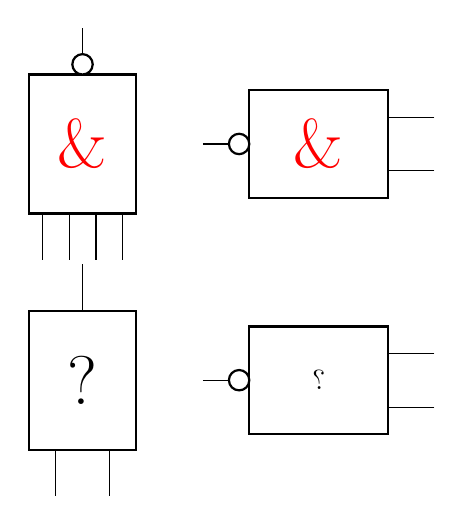
\begin{tikzpicture}
    \ctikzset{
        logic ports=european,
        logic ports origin=center,
        logic ports/scale=1.5,
        tripoles/european not symbol=ieee circle,
    }
    % Draw the Nand with big AND symbol
    \ctikzset{european ports font=\Huge\color{red}}
    \draw(0,0) node [nand port, rotate=90,
        number inputs=4]{};
    \draw(3,0) node [nand port, xscale=-1]{};
    % the un-rotation is not automatic for node text!
    \draw(0,-3) node [blank port, rotate=90,
        ]{\rotatebox{-90}{\Huge ?}};
    \draw(3,-3) node [blank not port, xscale=-1]{?};
\end{tikzpicture}
\end{LTXexample}

\paragraph{European logic port customization} Normally the European-style logic port with inverted output are marked with a small triangle; if you want you can change it with the key \texttt{tripoles/european not symbol}; its default is \texttt{triangle} but you can set it to \texttt{circle} like in the following example. As you can see, the circle size is the same as the circuit poles; if you prefer the size used in the IEEE standard ports, you can use set it to \texttt{ieee circle}.

\begin{LTXexample}[varwidth=true]
\begin{circuitikz}[european]
    \draw (0,3) node[nand port](A){}
        (A.out) to[short, *-o] ++(0.5,0);
    \ctikzset{tripoles/european not symbol=circle}
    \draw (0,1.5) node[nand port](A){}
        (A.out) to[short, *-o] ++(0.5,0);
    \ctikzset{tripoles/european not symbol=ieee circle}
    \draw (0,0) node[european nand port](A){}
        (A.out) to[short, *-o] ++(0.5,0);
\end{circuitikz}
\end{LTXexample}

In some standard, the \texttt{xnor} port is different --- without the negation at the end and with just an $=$ sign.\footnote{Suggested by user \texttt{Schlepptop} on GitHub.}
You can switch to this if you like, with the key \texttt{european xnor style} that can be \texttt{default} or \texttt{direct}.

\begin{LTXexample}[varwidth=true]
\begin{circuitikz}[european]
    \draw (0,0) node[xnor port]{};
    \ctikzset{european xnor style=direct}
    \draw (3,0) node[xnor port]{};
\end{circuitikz}
\end{LTXexample}

\paragraph{European logic port anchors} The anchors are basically the same as in the american-style ports.

\bigskip
\begin{circuitikz} [american]
\def\coorda(#1)<#2>{node[circle, red, draw, inner sep=1pt,pin={[red, overlay, inner sep=0.5pt, font=\small, pin distance=0.1cm, pin edge={red, overlay,}]#2:#1}](#1){}}

\draw (0, 0) node[european and port, ](A){} ;
  \foreach \a/\d in {left/45, right/45, center/-90}
    \path (A.\a) \coorda(\a)<\d>;

\draw (3,0) node[european and port, ](A){} ;
  \foreach \a/\d in {bin 1/-135, bin 2/-135, bout/-45}
    \path (A.\a) \coorda(\a)<\d>;

\draw (6,0) node[european nand port, ](A){} ;
  \foreach \a/\d in {bin 1/-135, bin 2/-135, bout/-45}
    \path (A.\a) \coorda(\a)<\d>;

\ctikzset{tripoles/european not symbol=circle}

\draw (9,0) node[european nand port, ](A){} ;
  \foreach \a/\d in {bin 1/-135, bin 2/-135, bout/-45}
    \path (A.\a) \coorda(\a)<\d>;

\end{circuitikz}
\bigskip


\subsection{Flip-flops}\label{sec:flipflops}

Flip-flops (available since version \texttt{1.0.0}) are an hybrid between the logic ports and the chips. They have a class by themselves (\texttt{flipflops}) but the default parameters are set at the same values as the logic gates one.

The default flip flop is empty: it is just a rectangular box like a blank \texttt{dipchip}  with 6 pins.
\begin{groupdesc}
    \circuitdesc*{flipflop}{Blank (void) flip flop}{FF}(
    pin 1/180/0.2, pin 2/180/0.2, pin 3/180/0.2,
    bpin 1/120/0.3, bpin 6/60/0.3, up/90/0.2, down/-90/0.2, bup/30/0.2, bdown/-30/0.2,
    pin 6/0/0.2, pin 5/0/0.2, pin 4/0/0.2)
\end{groupdesc}

As you can see, in a void flip flop no external pins are drawn: you have to define the meaning of each of them to see them.
To define a specific flip-flop, you have to set a series of keys under the \verb|\ctikzset| directory \texttt{multipoles/flipflop/}, corresponding to pins \texttt{1}\dots \texttt{6}, \texttt{u} for ``up'' and \texttt{d} for ``down'':
\begin{itemize}
    \item a \emph{text} value \texttt{t0}, \texttt{t1}, \dots \texttt{t6}, and \texttt{tu} and \texttt{td} (the last ones for up and down) which will set a label on the pin;
    \item a \emph{clock wedge} flag (\texttt{c0}, \dots  \texttt{c6}, \texttt{cu}, \texttt{cd}), with value \texttt{0} or \texttt{1}, which will draw a triangle shape on the border of the corresponding pin;
    \item a \emph{negation} flag (\texttt{n0}, \dots  \texttt{n6}, \texttt{nu}, \texttt{nd}),  with value \texttt{0} or \texttt{1}, which will put an \texttt{ocirc} shape on the outer border of the corresponding pin.
\end{itemize}

To set all these keys, an auxiliary style \texttt{flipflop def} is defined, so that you can do the following thing:

\begingroup
\tikzset{flipflop AB/.style={flipflop,
    flipflop def={t1=A, t3=B, t6=Q, t4={\ctikztextnot{Q}},
        td=rst, nd=1, c2=1, n2=1, t2={\texttt{CLK}}},
}}

\begin{lstlisting}
\tikzset{flipflop AB/.style={flipflop,
    flipflop def={t1=A, t3=B, t6=Q, t4={\ctikztextnot{Q}},
        td=rst, nd=1, c2=1, n2=1, t2={\texttt{CLK}}},
}}
\end{lstlisting}

to obtain:

\begin{groupdesc}
    \circuitdesc*{flipflop AB}{Example custom flip flop}{}(
    pin 1/180/0.2, pin 2/180/0.2, pin 3/180/0.2,
    bpin 1/120/0.3, bpin 6/60/0.3, down/-90/0.2, bdown/-30/0.2,
    pin 6/0/0.2)
\end{groupdesc}
\endgroup

\verb|\ctikztextnot{}| is a small utility macro to set a overbar to a text, like \ctikztextnot{RST} (created by \verb|\ctikztextnot{RST}|).


By default, the following flip-flops are defined, as well as a support shape for the clock wedge:
\begin{groupdesc}
    \circuitdesc*{latch}{D-type latch}{}
    \circuitdesc*{flipflop SR}{flip-flop SR}{}
    \circuitdesc*{flipflop D}{Edge-triggered synchronous flip-flop D}{}
    \circuitdesc*{flipflop T}{Edge-triggered synchronous flip-flop T}{}
    \circuitdesc*{flipflop JK}{Edge-triggered synchronous flip-flop JK}{}
    \circuitdesc{clockwedge}{clock wedge shape}{text}(center/180/0.6, nw/90/0.2, sw/-90/0.2, right/45/0.5)
\end{groupdesc}

If you prefer that the negated output is labelled \texttt{Q} and a dot indicating negation is shown, you can add the \texttt{dot on notQ} key:

\begin{groupdesc}
    \circuitdesc*{flipflop JK, dot on notQ}{synchronous flip-flop JK with asynchronous set and reset}{}
\end{groupdesc}

You can also  add ``vertical'' asynchronous set and reset (active low) adding the style \texttt{add async SR} to all of them:

\begin{groupdesc}
    \circuitdesc*{flipflop JK, add async SR}{synchronous flip-flop JK with asynchronous set and reset}{}
\end{groupdesc}

\subsubsection{Custom flip-flops}

If you like different pin distributions, you can easily define different flip-flops to your taste. For example, somebody likes the clock pin on the bottom pin:

\begingroup
\tikzset{flipflop myJK/.style={flipflop,
    flipflop def={t1=J, t2=K, t6=Q, t4={\ctikztextnot{Q}}, c3=1}}
}

\begin{lstlisting}
\tikzset{flipflop myJK/.style={flipflop,
    flipflop def={t1=J, t2=K, t6=Q, t4={\ctikztextnot{Q}}, c3=1}}
}
\end{lstlisting}

\begin{groupdesc}
    \circuitdesc*{flipflop myJK}{Example custom flip flop}{}
\end{groupdesc}
\endgroup

The standard definition of the default flip-flops are the following (in the file \texttt{pgfcircmultipoles.tex}):

\begin{lstlisting}[basicstyle=\small\ttfamily]
\tikzset{
    % async
    latch/.style={flipflop, flipflop def={t1=D, t6=Q, t3=CLK, t4=\ctikztextnot{Q}}},
    flipflop SR/.style={flipflop, flipflop def={t1=S, t3=R, t6=Q, t4=\ctikztextnot{Q}}},
    % sync
    flipflop D/.style={flipflop, flipflop def={t1=D, t6=Q, c3=1, t4=\ctikztextnot{Q}}},
    flipflop T/.style={flipflop, flipflop def={t1=T, t6=Q, c3=1, t4=\ctikztextnot{Q}}},
    flipflop JK/.style={flipflop,
                flipflop def={t1=J, t3=K, c2=1, t6=Q, t4=\ctikztextnot{Q}}},
    % additional features
    add async SR/.style={flipflop def={%
                tu={\ctikztextnot{SET}}, td={\ctikztextnot{RST}}}},
    dot on notQ/.style={flipflop def={t4={Q}, n4=1}},
}
\end{lstlisting}


\subsubsection{Flip-flops anchors}

Flip-flops have all the standard geometrical anchors, although it should be noticed that the external pins are \emph{outside} them. The pins are accessed by the number \texttt{1} to \texttt{6} for the lateral ones (like in DIP chips), and with the \texttt{up} and \texttt{down} anchors for the top and bottom one. All the pins have the ``border'' variant (add a \texttt{b} in front of them, no spaces).

\begin{quote}
        \geocoord{flipflop JK}\qquad
        \showanchors{flipflop JK, add async SR, external pins width=0.5}{}(%
            pin 1/180/0.5, pin 2/180/0.5, pin 3/180/0.5,
            up/90/0.2, down/-90/0.2,
            pin 6/0/0.5, pin 5/0/0.5, pin 4/0/0.5,
            bpin 1/120/0.3, bpin 2/135/0.3, bpin 3/-120/0.2,
            bup/30/0.3, bdown/-30/0.3,
            bpin 6/60/0.3, bpin 5/30/0.3, bpin 4/-30/0.4)
\end{quote}

If you have negated pins, you can access the \texttt{ocirc} shapes with the name as \texttt{\textsl{<nodename>}-N\textsl{<pin number>}}, and all the respective anchors (for example --- \verb|myFFnode-N4.west|).

\subsubsection{Flip-flops customization}\label{sec:flip-flop-cust}

Flip-flop's size is controlled by the class parameters (like \texttt{flipflops/scale})  and the specific \verb|\ctikzset| keys \texttt{multipoles/flipflop/width} and \texttt{multipoles/flipflop/pin spacing}. Class parameters are also used for line thickness and fill color. The default values are matched with the logic ports ones.

The fonts used for the pins \texttt{1}\dots \texttt{6} is set by the key \texttt{multipoles/flipflop/font} (by default \verb|\small| in \LaTeX{} and the equivalent in other formats) and the font used for pins \texttt{u} and \texttt{d} is \texttt{multipoles/flipflop/fontud} (\verb|\tiny| by default).
You can change it globally or specifically for each flip flop.

As in chips, you can change the length of the external pin with the key \texttt{external pins width}; you can for example have a pinless flip-flop like this:

\begin{groupdesc}
    \circuitdesc*{flipflop JK, add async SR, external pins width=0}{synchronous flip-flop JK}{}
\end{groupdesc}

Notice however that negated pins when the pins width is zero has to be handled with care. As explained in the poles sections, the \texttt{ocirc} shape is drawn at the end of the shape to cancel out the wires below; so if you use a pinless flipflop when you make the connection you should take care of connecting the symbol correctly. To this end, the shapes of the negation circles are made available as \texttt{\textsl{<nodename>}-N\textsl{<pin number>}}, as you can see in the next (contrived) example.


\begin{LTXexample}[varwidth=true]
\begin{circuitikz}[scale=3, transform shape]
    \clip (0.2,0.5) rectangle (1.2,-1.3);
    \node [flipflop JK,
           flipflop def={n5=1,n4=1,t5={/c},c5=1},
           external pins width=0,
           ](A){};
    \draw (A-N5.east) -- ++(1,0); % correct
    \draw (A.pin 4) -- ++(1,0);   % wrong
\end{circuitikz}
\end{LTXexample}

Normally the symbols on the flip-flop are un-rotated when you rotate the symbol, but as in case of chips, you can avoid it.

\begin{LTXexample}[pos=t]
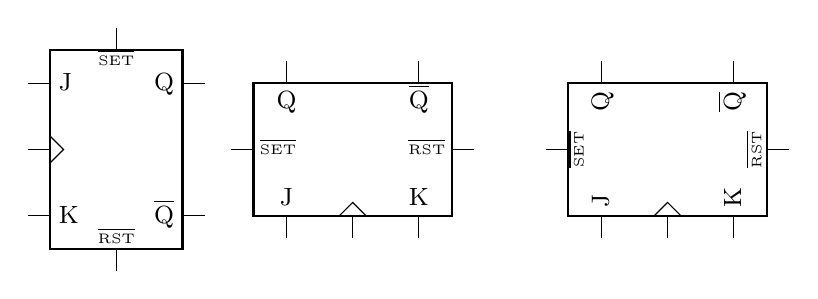
\begin{tikzpicture}
    \draw (0,0) node[flipflop JK, add async SR]{};
    \draw (3,0) node[flipflop JK, add async SR, rotate=90]{};
    \draw (7,0) node[flipflop JK, add async SR, rotate=90, rotated numbers]{};
\end{tikzpicture}
\end{LTXexample}

You can also change the size of the wedge, with the key \texttt{multipoles/flipflop/clock wedge size} (default value \texttt{0.2}).

\begin{LTXexample}[varwidth=true]
    \begin{circuitikz}[]
    \draw (0,0) node[flipflop JK]{JK};
    \ctikzset{multipoles/flipflop/clock wedge size=0.1}
    \draw (2.3,0) node[flipflop JK]{JK};
    \ctikzset{multipoles/flipflop/clock wedge size=0.4}
    \draw (4.6,0) node[flipflop JK]{JK};
\end{circuitikz}
\end{LTXexample}

Flip-flops ``not circles'' follows the current logic port setting (either if you choose \texttt{ieee ports}, or if you are using \texttt{european ports} with \texttt{european not symbol} set to \texttt{cirle} or \texttt{ieee circle}.

\begin{LTXexample}[varwidth=true]
\begin{circuitikz}[]
\ctikzset{logic ports=european,
    tripoles/european not symbol=ieee circle}
\draw (0,0) node[nand port](A){}
    (A.out) to[short] ++(0.5,0)
    node[flipflop JK, dot on notQ, anchor=pin 2]{JK};
\ctikzset{logic ports=european,
tripoles/european not symbol=circle}
\draw (0,-3) node[nand port](A){}
    (A.out) to[short] ++(0.5,0)
    node[flipflop JK, dot on notQ, anchor=pin 2]{JK};
\end{circuitikz}
\end{LTXexample}


\subsection{Multiplexer and de-multiplexer}\label{sec:muxdemuxes}

The shape used for muxes and de-muxes is probably the most configurable shape of the package; it has been added by Romano in \texttt{v1.0.0}. The basic shape is a multiplexer with 8 input pin, one output pin, and three control pins ($2^3\to1$ multiplexer). The pins are not named as input or output pins (see below for a full description for anchors) for reasons that will be clear later.

\begin{groupdesc}
    \circuitdesc*[0.7]{muxdemux}{mux-demux}{MD1}(lpin 1/180/0.2, lpin 2/180/0.2, bpin 1/-90/0.2, blpin 1/0/0.2, blpin 2/0/0.2, bbpin 1/90/0.2, rpin 1/0/0.1, brpin 1/-110/0.1)
    \circuitdesc{wedgeinv, scale=2}{Inversion marker for European logic symbols\footnotemark}{}(base/180/0.2, top/90/0.2, apex/0/0.2, mid/45/0.2, center/135/0.2)
    \footnotetext{Thanks for the contribution by \href{https://github.com/circuitikz/circuitikz/issues/679}{\texttt{yashpalgoyal1304} on GitHub}.}
    \circuitdesc{circleinv, scale=2}{Circle-shaped inversion marker}{}(base/180/0.2, top/90/0.2, apex/0/0.2, mid/45/0.2, center/135/0.2, bottom/-90/0.1)
\end{groupdesc}

You can define a custom shape for the \texttt{muxdemux}es using an interface similar to the one used in flip-flops; for example:

\begin{lstlisting}
\tikzset{demux/.style={muxdemux, muxdemux def={Lh=4, Rh=8, NL=1, NB=3, NR=8}}}
\end{lstlisting}

will generate the following shape (the definition above is already defined in the package):

\begin{groupdesc}
    \circuitdesc*[0.7]{demux}{Demultiplexer $1\to2^3$ with \texttt{Lh=4, Rh=8, NL=1, NB=3, NR=8} }{MD2}
\end{groupdesc}

The shape can also be defined with an inset. For example it can be used like this to define a 1-bit adder (also already available):

\begin{lstlisting}
\tikzset{one bit adder/.style={muxdemux,
         muxdemux def={Lh=4, NL=2, Rh=2, NR=1, NB=1, w=1.5,
         inset w=0.5, inset Lh=2, inset Rh=1.5}}}
\end{lstlisting}
\begin{groupdesc}
    \circuitdesc*{one bit adder}{One-bit adder}{\Large$\oplus$}
\end{groupdesc}

Or a Arithmetic Logic Unit (again, already defined by default):

\begin{lstlisting}
\tikzset{ALU/.style={muxdemux,
         muxdemux def={Lh=5, NL=2, Rh=2, NR=1, NB=2, NT=1, w=2,
         inset w=1, inset Lh=2, inset Rh=0, square pins=1}}}
\end{lstlisting}
\begin{groupdesc}
    \circuitdesc*{ALU}{ALU}{\rotatebox{90}{\small\ttfamily ALU}}
\end{groupdesc}

\subsubsection{Mux-Demux: design your own shape}

\begin{minipage}{0.45\linewidth}
\RaggedRight
In designing the shape there are several parameters to be taken into account. In the diagram on the right they are shown in a (hopefully) practical way. The parameter can be set in a node or in a style using the \texttt{muxdemux def} key as shown above, or set with \verb|\ctikzset| as \texttt{multipoles/muxdemux/Lh} keys and so on.
\end{minipage}%
\begin{minipage}{0.5\linewidth}
\centering
\begin{circuitikz}[quote/.style={thin, blue, <->}, refline/.style={red, dashed}]
    \def\myquotev#1#2#3#4{%
        \draw [refline] (A.#1) -- ++(#2,0) coordinate(tmp) --++(#3,0);
        \draw [quote] (tmp|-A.center) -- (tmp |- A.#1)
        node [midway, below=4pt, sloped, fill=white]{\texttt{#4}};
    }
    \def\myquoteh#1#2#3#4#5{%
        \draw [refline] (A.#1) -- ++(0,#2) coordinate(tmp) --++(0,#3);
        \draw [quote] (tmp) -- (tmp -| A.#5)
        node [right, fill=white]{\texttt{#4}};
    }
    \begin{scope}
        \clip (-4,-0.5) rectangle (2,3);
        \node [muxdemux, muxdemux def={NL=6, NR=3, NT=3,
        inset w=1.0, inset Lh=3.0, inset Rh=2.0}, no input leads](A) at(0,0) {};
        \draw [refline] (-4,0) -- (2,0);
        \draw [refline] (0,-1) -- (0,3);
    \end{scope}
    \myquotev{top left}{-2.8}{-.2}{Lh}
    \myquotev{inset top left}{-2.0}{-.2}{inset Lh}
    \myquotev{inset top right}{-1.4}{-.2}{inset Rh}
    \myquotev{top right}{.5}{.2}{Rh}
    \myquoteh{top left}{.3}{.2}{w}{center}
    \myquoteh{inset top left}{-1.5}{-.2}{inset w}{inset top right}
\end{circuitikz}
\end{minipage}

\bigskip

The default values are $\texttt{Lh}=8$, $\texttt{Rh}=6$, $\texttt{w}=3$ and no inset: $\texttt{inset Lh}=\texttt{inset Rh}=\texttt{inset w}=0$. In addition, you can set the following parameters:
\begin{description}
    \item [NL, NR, NB, NT]: number of pins relatively on the left, right, bottom and top side (default \texttt{8}, \texttt{1}, \texttt{3}, \texttt{0}). When an inset is active (in other words, when $\texttt{Lh}>0$) the pins are positioned on the top and bottom part, not in the inset; the exception is when the number of left pins is odd, in which case you have one pin set on the center of the inset.
    If you do not want a pin in one side, use \texttt{0} as number of pins.
    \item [square pins]: set to \texttt{0} (default) if you want the square pins to stick out following the slope of the bottom or top side, \texttt{1} if you want them to stick out in a square way (see the example above for the ALU).
\end{description}
All the distances are multiple of \texttt{multipoles/muxdemux/base len} (default \texttt{0.4}, to be set with \verb|\ctikzset|), which is relative to the basic length. That value has been chosen so that, if you have a number of pins which is equal to the effective distance where they are spread (which is \texttt{Lh} without inset, $\texttt{Lh}- (\texttt{inset Lh})$ with an inset), then the distance is the same as the default pin distance in chips, as shown in the next circuit. In the same drawing you can see the effect of \texttt{square pins} parameters (without it, the rightmost bottom lead of the \texttt{mux 4by2} shape will not connect with the below one).

\begin{LTXexample}[varwidth=true]
\begin{circuitikz}
    \tikzset{mux 4by2/.style={muxdemux,
        muxdemux def={Lh=4, NL=4, Rh=3,
        NB=2, w=2, square pins=1}}}
    \node [dipchip, num pins=8](A) at (0,0) {IC1};
    \node [one bit adder, scale=-1, anchor=lpin 2]
        at (A.pin 1){};
    \node [mux 4by2, anchor=lpin 1](B)
        at (A.pin 8){MUX};
    \node [qfpchip, num pins=8, anchor=pin 8] at
        (B.bpin 1) {IC2};
\end{circuitikz}
\end{LTXexample}

\subsubsection{Mux-Demux customization}

Mux-demuxes have the normal parameters of their class (\texttt{muxdemuxes}):  you can scale them with the \verb|\ctikzset| key \texttt{muxdemuxes/scale}, control the border thickness with \texttt{muxdemuxes/thickness} and the default fill color with  \texttt{muxdemuxes/fill} --- they are set, by default, at the same values than \texttt{logic ports}.

External pins' length is controlled by the key \texttt{multipoles/external pins width} (default \texttt{0.2}) or by the style \texttt{external pins width}. The parameter
\texttt{multipoles/external pins thickness} is also respected.
like in chips. In addition, like in logic ports, you can suppress the
drawing of the leads by using the boolean key
\texttt{logic ports draw input leads} (default \texttt{true}) or, locally,
with the style \texttt{no inputs leads} (that can be reverted with
\texttt{input leads}).
The main difference between setting \texttt{external pins width} to \texttt{0} or using \texttt{no inputs lead} is that in the first case the normal pin anchors and the border anchors will coincide, and in the second case they will not move and stay where they should have been if the leads were drawn.

You can draw only selected pins and leave out the rest by setting the keys
\texttt{multipoles/draw only \emph{side} pins} and the corresponding style
\texttt{draw only \emph{side} pins} where \texttt{\emph{side}} can be \texttt{left}, \texttt{right},
\texttt{top}, \texttt{bottom}.
Those key accept a comma-separated list of
pin numbers or ranges of pin numbers (a range is given as
\texttt{$\langle$start$\rangle$ - $\langle$end$\rangle$}, ends are inclusive).
The numbers will not be expanded in any way, except those given as ends of
ranges. A special value (and the initial one) is \texttt{all}, in which case all
pins are drawn. The anchors will be adjusted, such that each \texttt{\emph{x}pin
\textit{n}} will be placed at the end of the pins which are drawn, and coincide
with the \texttt{b\emph{x}pin \textit{n}} anchors for the suppressed pins.

\begin{LTXexample}[varwidth=true]
    \begin{circuitikz}
    \node [muxdemux, muxdemux def={NL=4, NR=3, NT=5, NB=3, w=2,
            inset w=0.5, Lh=4, inset Lh=2.0, inset Rh=1.0,
            square pins=1},
        draw only right pins={1,3},
        draw only top pins={1-3},
        draw only bottom pins={3}](C) at (0,0) {X};
    \end{circuitikz}
\end{LTXexample}

\subsubsection{Mux-Demux anchors}

Mux-demuxes have a plethora of anchors. As in the case of chips, the geographic anchors mark the rectangle occupied by the component, without taking into account the pin leads.

\begin{quote}
    \scalebox{0.7}{%
        \geocoord[baseline=(N.center)]{muxdemux}
        \showanchors[baseline=(N.center)]{muxdemux}{X}(top left/180/0.3, top/90/0.3, top right/0/0.3,
        bottom left/180/0.3, bottom/-90/0.3, bottom right/0/0.3, left/180/0.3, right/0/0.3,
        center/45/0.2, center up/0/0.4, center down/0/0.4)
        \showanchors[baseline=(N.center)]{muxdemux, muxdemux def={NL=6, NR=3, NT=3, inset w=1.0,
        inset Lh=3.0, inset Rh=2.0}, no input leads}{}(inset top left/180/0.3, inset top/90/0.5,
        inset top right/0/0.3, inset bottom left/180/0.3, inset bottom/-90/0.5,
        inset bottom right/-20/0.3, inset left/180/0.3, inset right/-20/0.2, inset center/135/0.2,
        narrow center/20/0.2, center up/45/0.4, center down/-45/0.4)
}
\end{quote}

The pins anchors are named \texttt{lpin}, \texttt{rpin}, \texttt{bpin} and \texttt{tpin} for the left, right, bottom and top pin respectively, and points to the ``external'' pin. The border pins are named the same, with a \texttt{b} added in front: \texttt{blpin}, \texttt{brpin}, \texttt{bbpin} and \texttt{btpin}.
The following graph will show the numbering and position of the pin anchors.

\begin{quote}
\begin{circuitikz}
    \node [muxdemux, muxdemux def={NL=4, NR=3, NT=3, NB=3, w=2, inset w=0.5,
        Lh=4, inset Lh=2.0, inset Rh=1.0, square pins=1}](C) at (0,0) {X};
    \node [muxdemux, muxdemux def={NL=7, NR=8, NT=4, inset w=1.0,
        inset Lh=4.0, inset Rh=0.0}](D) at (4,0) {X};
    \foreach \myn/\NL/\NR/\NB/\NT in {C/4/3/3/3,D/7/8/3/4} {
        \foreach \myp in {1,...,\NL} \node[right, font=\tiny] at (\myn.blpin \myp){\myp};
        \foreach \myp in {1,...,\NR} \node[left, font=\tiny] at(\myn.brpin \myp) {\myp};
        \foreach \myp in {1,...,\NB} \node[above, font=\tiny] at (\myn.bbpin \myp){\myp};
        \foreach \myp in {1,...,\NT} \node[below, font=\tiny] at (\myn.btpin \myp){\myp};
    }
    \path (C.lpin 1) \showcoord(lpin 1)<180:0.3>;
    \path (D.blpin 1) \showcoord(blpin 1)<135:0.3>;
    \path (C.tpin 1) \showcoord(tpin 1)<180:0.3>;
    \path (D.btpin 1) \showcoord(btpin 1)<45:0.3>;
    \path (C.rpin 1) \showcoord(rpin 1)<0:0.3>;
    \path (D.brpin 1) \showcoord(brpin 1)<45:0.3>;
    \path (C.bpin 2) \showcoord(bpin 2)<-90:0.3>;
    \path (C.bbpin 2) \showcoord(bbpin 2)<-60:0.3>;
    \path (D.bbpin 2) \showcoord(bbpin 2)<-45:0.3>;
\end{circuitikz}
\end{quote}


The code that implemented the printing of the numbers (which in \texttt{muxdemux}es, differently from chips, are never printed automatically) in the last graph is the following one.

\begin{lstlisting}[basicstyle=\small\ttfamily]
\begin{circuitikz}
\node [muxdemux, muxdemux def={NL=4, NR=3, NT=3, NB=3, w=2, inset w=0.5,
    Lh=4, inset Lh=2.0, inset Rh=1.0, square pins=1}](C) at (0,0) {X};
\node [muxdemux, muxdemux def={NL=7, NR=8, NT=4, inset w=1.0,
    inset Lh=4.0, inset Rh=0.0}](D) at (4,0) {X};
\foreach \myn/\NL/\NR/\NB/\NT in {C/4/3/3/3,D/7/8/3/4} {
    \foreach \myp in {1,...,\NL} \node[right, font=\tiny] at (\myn.blpin \myp){\myp};
    \foreach \myp in {1,...,\NR} \node[left, font=\tiny] at(\myn.brpin \myp) {\myp};
    \foreach \myp in {1,...,\NB} \node[above, font=\tiny] at (\myn.bbpin \myp){\myp};
    \foreach \myp in {1,...,\NT} \node[below, font=\tiny] at (\myn.btpin \myp){\myp};
}
\end{lstlisting}

\subsubsection{Adding wedge or circular inversion markers}\label{sec:wedge-inversion}

Although you can add ``negation balls'' as seen for, for example, flip-flops (see section~\ref{sec:flip-flop-cust}), sometimes the European-style notation (also accepted by the IEEE standard) with the small wedge is preferred. The \texttt{wedgeinv} shape will nicely do. It'll scale with the \texttt{muxdemuxes} class, and the length and height can be changed with the keys \texttt{wedge inversion mark/width} (default \texttt{0.2}) and \texttt{height} (default \texttt{0.1}), with the same units that are used for the \texttt{external pins width} and similar keys.

Similarly, there is also a \texttt{circleinv} shape, which is basically the same as the \texttt{notcirc} (see~\ref{sec:ieeestdports}) one, but that scales with the \texttt{muxdemuxes} class and that has the default anchor at its left, similarly to \texttt{wedgeinv}. This one will be filled if the class says so, contrary to the wedge-like shapes that are always open.

\begin{LTXexample}[varwidth=true]
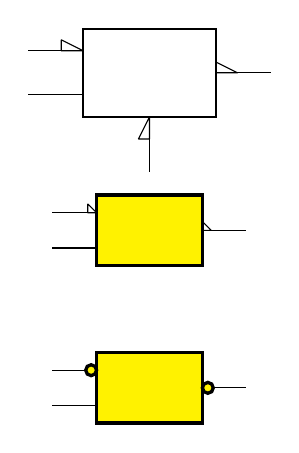
\begin{tikzpicture}[]
    \path (0,4) node[muxdemux, muxdemux def={NL=2,Lh=2,Rh=2,NB=1},
        external pins width = 0.5](mdemux){};
    \draw (mdemux.blpin 1) node[wedgeinv,anchor=apex]{};
    \draw (mdemux.brpin 1) node[wedgeinv]{};
    \draw (mdemux.bbpin 1) node[wedgeinv, anchor=apex,
        rotate=90]{};
    \ctikzset{wedge inversion mark/.cd, width=0.1}
    \ctikzset{muxdemuxes/.cd, fill=yellow, thickness=3, scale=0.8}
    \path (0,2) node[muxdemux, muxdemux def={NL=2,Lh=2,Rh=2,NB=0},
        external pins width = 0.5](mdemux){};
    \draw (mdemux.blpin 1) node[wedgeinv,anchor=apex]{};
    \draw (mdemux.brpin 1) node[wedgeinv]{};
    \path (0,0) node[muxdemux, muxdemux def={NL=2,Lh=2,Rh=2,NB=0},
        external pins width = 0.5](mdemux){};
    \draw (mdemux.blpin 1) node[circleinv,anchor=apex]{};
    \draw (mdemux.brpin 1) node[circleinv]{};
\end{tikzpicture}
\end{LTXexample}

\subsubsection{Mux-Demux special usage}

You can use these shapes  to draw a lot of symbols that are unavailable; using a bit of \LaTeX{} command trickery you can use them quite naturally too\dots. Examples with personalized amplifier shapes are listed in section~\ref{sec:muxdemux-amplis}.

As an additional example, this was used before the introduction of the \texttt{double tgate} symbol in \texttt{1.2.4} (see ~\ref{sec:passgate}):

\begin{LTXexample}[varwidth=true]
\def\tgate#1{
    node[simple triangle, anchor=left, no input leads](#1-LR){}
    (#1-LR.right) node[simple triangle, xscale=-1,
    anchor=left](#1-RL){}
    ([yshift=.5ex]#1-RL.btpin 1) node[ocirc]{}}
\begin{circuitikz}[
    simple triangle/.style={muxdemux, muxdemux def={
            NL=1, NR=1, NB=1, NT=1, w=2, Lh=2, Rh=0,
    }}]
    \draw (0,0) \tgate{A} (0,-2) \tgate{B};
    \draw (A-RL.bpin 1) -- (B-RL.tpin 1);
\end{circuitikz}
\end{LTXexample}

Finally, you can play with them to create chips that have generic numbers of pins on the four sides, as in the following example (asked on \href{https://tex.stackexchange.com/q/596320/38080}{TeX.Stackexchange}):

\begin{LTXexample}[varwidth=true]
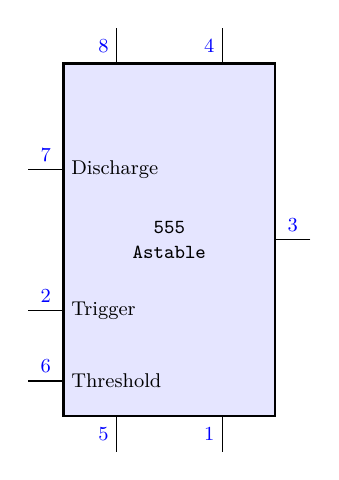
\begin{tikzpicture}[scale=0.8, transform shape]
    \tikzset{ic555/.style={muxdemux,
            muxdemux def={Lh=10, NL=5, Rh=10, NR=5,
            NB=2, w=6, NT=2, square pins=1},
        no input leads, external pins width=0.4,
        circuitikz/muxdemuxes/fill=blue!10}
    }
    \node [ic555, font=\small\ttfamily,align=center](A)
        at (0,0) {555\\Astable};
    % left pins
    \foreach \rawpin/\npin/\label in
        {2/7/Discharge, 4/2/Trigger, 5/6/Threshold} {
        \draw (A.lpin \rawpin) -- (A.blpin \rawpin)
            node[midway, blue, font=\small, above]{\npin}
            node[right, font=\small]{\label};
    }
    % top pins
    \foreach \rawpin/\npin in {1/8, 2/4} {
        \draw (A.tpin \rawpin) -- (A.btpin \rawpin)
            node[midway, blue, font=\small, left]{\npin};
    }
    % bottom pins
    \foreach \rawpin/\npin in {1/5, 2/1} {
        \draw (A.bpin \rawpin) -- (A.bbpin \rawpin)
            node[midway, blue, font=\small, left]{\npin};
    }
    % finally, left
    \draw (A.rpin 3) -- (A.brpin 3)
        node[midway, blue, font=\small, above]{3};
\end{tikzpicture}
\end{LTXexample}


\subsection{Chips (integrated circuits)}\label{sec:chips}

\texttt{CircuiTikZ} supports two types of variable-pin chips: DIP (Dual-in-Line Package) and QFP (Quad-Flat Package).
\begin{groupdesc}
    \circuitdesc*{dipchip}{Dual-in-Line Package chip}{}
    \circuitdesc*{qfpchip}{Quad-Flat Package chip}{}
\end{groupdesc}

\subsubsection{DIP and QFP chips customization}

You can scale chips with the key \texttt{chips/scale}. As ever, that will \textbf{not} scale text size of the labels, when they are printed.

The line thickness of the main shape is controlled by \texttt{multipoles/thickness} (default 2) and the one of the external pins/pads with \texttt{multipoles/external pins thickness} (default 1).

You can customize the DIP chip with the key \texttt{multipoles/dipchip/width} (with a default of \texttt{1.2}) and  the key \texttt{multipoles/dipchip/pin spacing} (default \texttt{0.4}) that are expressed in fraction of basic lengths (see section~\ref{sec:components-size}).
The height of the chip will be equal to half the numbers of pins multiplied by the spacing, plus one spacing for the borders.

For the QFP chips, you can only chose the pin spacing with \texttt{multipoles/qfpchip/pin spacing} key.

The number of pins is settable with the key \texttt{num pins}.
\textbf{Please notice} that the number of pins \textbf{must} be \emph{even} for \texttt{dipchip}s and \emph{multiple of 4} for \texttt{qfpchip}s, otherwise havoc will ensue.

The pins of the chip can be ``hidden'' (that is, just a spot in the border, optionally marked with a number) or ``stick out'' with a thin lead by setting \texttt{multipoles/external pins width} greater than 0 (default value is \texttt{0.2}, so you'll have leads as shown above).
Moreover, you can transform the thin lead into a pad by setting the key \texttt{multipoles/external pad fraction} to something different form 0 (default is \texttt{0}); the value expresses the fraction of the pin spacing space that the pad will use on both sides of the pin.

You can, if you want, avoid printing the numbers of the pin with \texttt{hide numbers} (default \texttt{show numbers}) if you prefer positioning them yourself (see the next section for the anchors you can use).

\begin{LTXexample}[varwidth=true]
    \begin{circuitikz}
        \ctikzset{multipoles/thickness=4}
        \ctikzset{multipoles/external pins thickness=2}
        \draw (0,0) node[dipchip,
          num pins=12,
          hide numbers,
          external pins width=0.3,
          external pad fraction=4 ](C){IC1};
        \draw (C.pin 1) -- ++(-0.5,0) to[R]
          ++(0,-3) node[ground]{};
          \node [right, font=\tiny]
          at (C.bpin 1) {RST};
    \end{circuitikz}
\end{LTXexample}


Also, you can suppress the drawing of the pins, by using the style \texttt{no inputs leads} (that can be reverted with \texttt{input leads}). The main difference between setting \texttt{external pins width} to \texttt{0} or using \texttt{no inputs lead} is that in the first case the normal pin anchors and the border anchors will coincide, and in the second case they will not move and stay where they should have been if the leads were drawn.

For special use you can suppress the orientation mark with the key \texttt{no topmark} (default \texttt{topmark}).

\begin{LTXexample}[varwidth=true]
    \begin{circuitikz}
        \draw (0,0) node[dipchip,
          num pins=8, no topmark,
          external pins width=0.0](C){IC1};
        \draw (C.pin 1) -- ++(-0.5,0) to[R]
          ++(0,-1.5) node[ground]{};
    \end{circuitikz}
\end{LTXexample}

The font used for the pins is adjustable with the key \texttt{multipoles/font} (default \verb|\tiny|)

\begin{LTXexample}[varwidth=true]
    \begin{circuitikz}
        \ctikzset{multipoles/font={\color{red}\tiny}}
        \draw (0,0) node[qfpchip,
          num pins=16,
          external pad fraction=6](C){IC1};
        \draw (C.pin 1) -- ++(-0.5,0) to[R]
          ++(0,-2) node[ground]{};
    \end{circuitikz}
\end{LTXexample}

You can draw only selected pins and leave out the rest by setting
\texttt{multipoles/draw only pins}\footnote{Added by
\href{https://github.com/circuitikz/circuitikz/pull/550}{Jonathan P. Spratte in \texttt{v1.3.8}}}.
This key accepts a comma-separated list of
pin numbers or ranges of pin numbers (a range is given as
\texttt{$\langle$start$\rangle$ - $\langle$end$\rangle$}, ends are inclusive).
The numbers will not be expanded in any way, except those given as ends of
ranges. A special value (and the initial one) is \texttt{all}, in which case all
pins are drawn. The anchors will be adjusted, such that each \texttt{pin
\textit{n}} will be placed at the end of the pins which are drawn, and coincide
with the \texttt{bpin \textit{n}} anchors for the suppressed pins.


\begin{LTXexample}[varwidth=true]
    \begin{circuitikz}
        \draw (0,3) node[dipchip,
        num pins=8,
        draw only pins={1, 3, 5-8}](C){IC1};
        \draw (C.pin 1) -- ++(-0.5,0) to[R]
        ++(0,-1.5) node[ground]{};
        \foreach \x in {1,...,8} {
            \draw[red] (C.pin \x) circle[radius=2pt];
            \draw[blue] (C.bpin \x) circle[radius=1pt];
        }
        \draw (0, 0) node[qfpchip, draw only pins={1-2, 6, 8, 4},
             external pad fraction=4, num pins=12](Q){};
        \foreach \x in {1,...,12} {
            \draw[red] (Q.pin \x) circle[radius=2pt];
            \draw[blue] (Q.bpin \x) circle[radius=1pt];
        }
    \end{circuitikz}
\end{LTXexample}

\subsubsection{Chips anchors}

Chips have anchors on pins and global anchors for the main shape.
The pin anchors to be used to connect wires to the chip are called \texttt{pin 1}, \texttt{pin 2} , \dots, with just one space between \texttt{pin} and the number.
Border pin anchors (\texttt{bpin 1}\dots) are always on the box border, and can be used to add numbers or whatever markings are needed.
Obviously, in case of \texttt{multipoles/external pins width} equal to zero, border and normal pin anchors will coincide.

Additionally, you have geometrical anchors on the chip ``box'', see the following figure. The nodes are available with the full name (like \texttt{north}) and with the short abbreviations \texttt{n}, \texttt{nw}, \texttt{w}\dots. The \texttt{dot} anchor is useful to add a personalized marker if you use the \texttt{no topmark} key.

\begin{quote}
    \bigskip
    \def\coord(#1){node[circle, red, draw,  inner sep=1pt,pin={[red, overlay, inner sep=0.5pt, font=\scriptsize, pin distance=0.2cm, fill=white, fill opacity=0.5, text opacity=1, pin edge={red, overlay,}]75:#1}](#1){}}
    \def\coordd(#1){node[circle, red, draw,  inner sep=1pt,pin={[red, overlay, inner sep=0.5pt, font=\scriptsize, pin distance=0.2cm, fill=white, fill opacity=0.5,  text opacity=1,pin edge={red, overlay,}]-45:#1}](#1){}}
    \begin{circuitikz}[american, ]
        \ctikzset{multipoles/dipchip/pin spacing=0.7}
        \draw (0,0) node[dipchip,
            external pins width=0.4,
            external pad fraction=4](C){IC1};
        \foreach \p in {1,...,8}
            \path (C.pin \p) \coord(pin \p)
            (C.bpin \p) \coordd(bpin \p);
        % second chip
        \draw (C.pin 7) to[R] ++(3,0)
              node[dipchip,anchor=pin 2](D){IC2};
        \foreach \p in {center, nw, ne, se, sw, north, south, west, east}
            \path (D.\p) \coord(\p);
        \path (D.text) \coordd(text);
        % third chip
        \draw (D.pin 7)  ++(2,0)
              node[dipchip,anchor=pin 2, no topmark](E){};
        \foreach \p in {center, n, w, e, s, dot}
            \path (E.\p) \coord(\p);
    \end{circuitikz}
\end{quote}

\subsubsection{Chips rotation}

You can rotate chips, and normally the pin numbers are kept straight (option \texttt{straight numbers}, which is the default), but you can rotate them if you like with \texttt{rotated numbers}.
Notice that the main label has to be (counter-) rotated manually in this case.

\begin{LTXexample}[varwidth=true]
\begin{circuitikz}
    \draw (0,0) node[dipchip,
        rotate=90]{%
        \rotatebox{-90}{IC2}};
    \draw (3,0) node[qfpchip,
        rotated numbers,
        rotate=45]{IC3};
\end{circuitikz}
\end{LTXexample}

\subsubsection{Chip special usage}

You can use chips to have special, personalized blocks.
Look at the following example, which is easily put into a macro.

\begin{LTXexample}[varwidth=true]
\begin{circuitikz}
    \ctikzset{multipoles/thickness=3}
    \ctikzset{multipoles/dipchip/width=2}
    \draw (0,0) node[dipchip,
        num pins=10, hide numbers, no topmark,
        external pins width=0](C){Block};
    \node [right, font=\tiny] at (C.bpin 1) {RST};
    \node [right, font=\tiny] at (C.bpin 2) {IN1};
    \node [right, font=\tiny] at (C.bpin 4) {/IN2};
    \node [left, font=\tiny]  at (C.bpin 8) {OUT};
    \draw (C.bpin 2) -- ++(-0.5,0) coordinate(extpin);
    \node [ocirc, anchor=0](notin2) at (C.bpin 4) {};
    \draw (notin2.180) -- (C.bpin 4 -| extpin);
    \draw (C.bpin 8) to[short,-o] ++(0.5,0);
    \draw (C.bpin 5) ++(0,0.1) -- ++(0.1,-0.1)
        node[right, font=\tiny]{CLK} -- ++(-0.1,-0.1);
    \draw (C.n) -- ++(0,1) node[vcc]{};
    \draw (C.s) -- ++(0,-1) node[ground]{};
\end{circuitikz}\end{LTXexample}

\subsection{Seven segment displays}

\begin{groupdesc}
    \circuitdesc*{bare7seg}{Seven segment display}{}
\end{groupdesc}

The seven-segment display lets you show values as if they were displayed in a classical seven-segment display.\footnote{This component has been loosely inspired by the package \texttt{SevenSeg} by Germain Gondor, 2009, see \href{http://www.texample.net/tikz/examples/seven-segment-display/}{\TeX{}example.net}.}

The main ``bare'' component is the one shown above, but for simplicity a couple of style interfaces are defined:

\begin{LTXexample}[varwidth=true]
\begin{circuitikz}
    \draw (0,0) node[seven segment val=A dot off box on]{};
    \draw (1,0) node[seven segment val=- dot none box on]{};
    \draw (0,-2) node[seven segment bits=1001001 dot empty box on]{};
    \draw (1,-2) node[seven segment bits=0011101 dot none box off]{};
\end{circuitikz}
\end{LTXexample}

There are two main configuration methods. The first one is \texttt{seven segment val}, which will take an hexadecimal number or value and display it: the possible values are \texttt{0,...,15}, plus \texttt{A, B, C, D, E, F} (or lowercase) and the symbol \texttt{-} (minus).


The other interface is \texttt{seven segment bits}, where you specify seven bits saying which segment must be on (please never specify a different number of bits, it will throw a very obscure error); you can see in the anchors the name of each segment.

The option \texttt{dot} specifies if you want a decimal dot or not. The key \texttt{none} will remove the dot and the space it would take; \texttt{empty} will not show the dot at all but reserve the space, and \texttt{on} or \texttt{off} will show the dot in the corresponding state.

The option \texttt{box} (can be \texttt{on} or \texttt{off}) simply toggles the drawing of the external box. You can separate it from the display with the key \texttt{seven seg/box sep} (default \texttt{1pt}), and it will use the thickness specified in \texttt{multipoles/thickness} (The same as the chips).

You can use these option with the ``bare'' object \texttt{bare7seg} and the keys \texttt{seven seg/bits} (default \texttt{0000000}), \texttt{seven seg/dot} (default \texttt{none}) and \texttt{seven seg/box} (default \texttt{off}); there is no option equivalent to the \texttt{val} interface.

\subsubsection{Seven segments anchors}

These are the anchors for the seven-segment displays; notice that when the \texttt{dot} parameter is not \texttt{none}, the cell is a bit wider at the right side.

\begingroup
\ctikzset{seven seg/color off=gray, multipoles/thickness=1}
\showanchors{bare7seg}{}(north/90/0.4, north east/45/0.4, east/0/0.4,
south east/-45/0.4, south/-90/0.4, south west/-135/0.4, west/180/0.4,
north west/135/0.4, center/-140/0.5)
\ctikzset{seven seg/dot=off}
\ctikzset{seven seg/box=on}
\showanchors{bare7seg}{}(north/90/0.4, north east/45/0.4, east/0/0.4,
south east/-45/0.4, south/-90/0.4, center/-140/0.5)
\ctikzset{seven seg/box=off}
\showanchors{bare7seg}{}(a/90/0.4, b/45/0.4, c/0/0.4, d/-90/0.4,
e/-129/0.4, f/145/0.4, g/190/0.4, dot/-45/0.2)
\endgroup

\subsubsection{Seven segments customization}

You can scale the seven segment  display with the key \texttt{displays/scale}. This will scale the size of the digit, but not the absolute sizes shown below --- if you want them to scale, yo have to do it manually.

You can change several parameters to adjust the displays:
\begin{lstlisting}[basicstyle=\small\ttfamily]
\ctikzset{seven seg/width/.initial=0.4}% relative to \pgf@circ@Rlen (scalable)
\ctikzset{seven seg/thickness/.initial=4pt}% segment thickness (not scaled)
\ctikzset{seven seg/segment sep/.initial=0.2pt}% gap between segments (not scaled)
\ctikzset{seven seg/box sep/.initial=1pt}% external box gap (not scaled)
\ctikzset{seven seg/color on/.initial=red}% color for segment "on"
\ctikzset{seven seg/color off/.initial=gray!20!white} % ...and "off"
\end{lstlisting}

A couple of examples are shown below.

\begin{LTXexample}[varwidth=true, pos=b]
\begin{circuitikz}[scale=0.5]
\ctikzset{seven seg/width=0.2, seven seg/thickness=2pt}
\foreach \i in {0,...,15} \path (\i,0)
    node[seven segment val=\i dot on box off]{};
\ctikzset{seven seg/color on=black}
\foreach \i in {0,...,15} \path (\i,-1.5)
    node[seven segment val=\i dot off box off, fill=gray!30!white]{};
\ctikzset{seven seg/color on=green, seven seg/color off=yellow!30}
\foreach \i in {0,...,15} \path[color=red] (\i,-3)
    node[seven segment val=\i dot none box on, xslant=0.2]{};
\end{circuitikz}
\end{LTXexample}



\section{Labels, voltages and currents}

You can add ``decorations'' to the path-style components; there are basically five types of them: labels, annotations, voltages, currents, and flows. Let's see an example of all of them\dots

\begin{LTXexample}[varwidth=true]
\begin{circuitikz}
   \draw (0,0) to[R, l=$R_1$, f=$i_1$] (2,0);
\end{circuitikz}
\end{LTXexample}

\begin{LTXexample}[varwidth=true]
\begin{circuitikz}
    \draw (0,0) to[R=$R_1$, a=\SI{1}{\kohm}] (2,0);
\end{circuitikz}
\end{LTXexample}


\begin{LTXexample}[varwidth=true]
\begin{circuitikz}
   \draw (0,0) to[R, i=$i_1$] (2,0);
\end{circuitikz}
\end{LTXexample}

\begin{LTXexample}[varwidth=true]
\begin{circuitikz}
   \draw (0,0) to[R, v=$v_1$] (2,0);
\end{circuitikz}
\end{LTXexample}

\begin{LTXexample}[varwidth=true]
\begin{circuitikz}
   \draw (0,0) to[R=$R_1$, i=$i_1$, v=$v_1$] (2,0);
\end{circuitikz}
\end{LTXexample}

\begin{LTXexample}[varwidth=true]
\begin{circuitikz}
   \draw (0,0) to[R=$R_1$, i=$i_1$, v=$v_1$] (2,0);
\end{circuitikz}
\end{LTXexample}


Long names/styles for the bipoles can be used, of course, and there is a special syntax (that works only in simple cases, and olny with \LaTeX{} --- use it with caution!) if you load the package with the `siunitx` options:

\begin{LTXexample}[varwidth=true]
\begin{circuitikz}\draw
  (0,0) to[resistor=1<\kilo\ohm>] (2,0);
\end{circuitikz}
\end{LTXexample}

\subsection{Labels and Annotations}
\label{sec:labels-and-annotations}
Since Version 0.7, beside the original label (\texttt{l})  option, there is a new option to place a second label, called annotation (\texttt{a}) at each bipole.

\subsubsection{Label and annotation position}
When drawing a component left-to-right, the label \texttt{l} is by default above the component, and the annotation \texttt{a} is by default below it. The position of annotations and labels can be adjusted adding the characters \verb|_| or \verb|^| to the key.

\begin{LTXexample}[varwidth=true]
\begin{circuitikz}
   \draw (0,0) to[R, l=$R_1$,a=1<\kilo\ohm>] (2,0);
\end{circuitikz}
\end{LTXexample}

\begin{LTXexample}[varwidth=true]
\begin{circuitikz}
   \draw (0,0) to[R, l_=$R_1$,a^=1<\kilo\ohm>] (2,0);
\end{circuitikz}
\end{LTXexample}

For passive components, you can use \texttt{\emph{component type}=text} as a shortcut for \texttt{\emph{component type}, l=text}:

\begin{LTXexample}[varwidth=true]
\begin{circuitikz}
   \draw (0,0) to[R=$R_1$,a=1<\kilo\ohm>] (2,0);
\end{circuitikz}
\end{LTXexample}

Notice though that in active component (sources of either voltage or current) the shortcut will set the voltage (\texttt{v}) or current (\texttt{i}) property.

\paragraph{Adjust label and annotation position.}\label{sec:adjust-label-position}
Normally the package will guess a good position for the label or annotation; if you do not like it,
you can add\footnote{Since version \texttt{1.3.3}} (or remove, with negative values) distance using the \verb|\ctikzset| keys \texttt{label distance} and \texttt{annotation distance}.

\begin{LTXexample}[varwidth=true]
\begin{circuitikz}
    \draw (0,0) to[sR, l=$R$, label distance=-4pt] (2,0)
    to [sR, l=$R$] (4,0);
\end{circuitikz}
\end{LTXexample}

\begin{LTXexample}[varwidth=true]
\begin{circuitikz}[american]
    \ctikzset{bipoles/inductors/core distance=4pt}
    \draw (0,1) to[L=$L$, name=myL] ++(2,0);
    \draw[thick, double] (myL.core west) -- (myL.core east);
    \draw (0,0) to[L=$L$, name=myL, label distance=2pt] ++(2,0);
    \draw[thick, double] (myL.core west) -- (myL.core east);
\end{circuitikz}
\end{LTXexample}

\subsubsection{Special symbols in labels and annotations.}\label{sec:bracing-of-labels}
When \TikZ{} processes the options, there will be problems if the label (or annotation, voltage, or current) contains one of the characters $=$ (equal) or $,$ (comma) --- because the parser search for those two characters to delimit the arguments, giving unexpected errors and wrong output.
These two characters can be protected from the option parser using an extra set of braces.

\begin{LTXexample}[varwidth=true]
    \begin{circuitikz}
        % the following will fail:
        % \draw (0,0) to[R, l=$R=3$]
        \draw (0,0) to[R, l={$R=3$}] (3,0);
        \draw (0,0) to[R={$R=3$}] (0,3);
        \draw (3,3) to[R={$R,3$}] (3,0);
        % this works, but it has wrong spacing
        \draw (0,3) to[R, l=$R{=}3$] (3,3);
    \end{circuitikz}
\end{LTXexample}

\textbf{Caveat:} up to version \texttt{1.2.7}, due to the way in which \Circuitikz{} used to processes the options, even that was not sufficient, so you must protect that tokens even more, for example using an \verb|\mbox| command, or redefining the characters with a \TeX\ \verb|\def|:

\begin{LTXexample}[varwidth=true]
    \begin{circuitikz}
        \def\eq{=}
        % the following will fail up to 1.2.7:
        % \draw (0,0) to[R, l={$R=3$}] (3,0);
        \draw (0,0) to[R, l=\mbox{$R=3$}] (3,0);
        \draw (0,0) to[R, l=$R\eq3$] (0,3);
        \draw (3,3) to[R, l=\mbox{$R,3$}] (3,0);
        % this works, but it has wrong spacing
        \draw (0,3) to[R, l=$R{=}3$] (3,3);
    \end{circuitikz}
\end{LTXexample}


\subsubsection{Labels and annotation orientation.}
The default orientation of labels is controlled by the options \texttt{smartlabels}, \texttt{rotatelabels} and \texttt{straightlabels} (or the corresponding \texttt{label/align} keys). Here are examples to see the differences:
\begin{LTXexample}[varwidth=true]
\begin{circuitikz}
\ctikzset{label/align = straight}
\def\DIR{0,45,90,135,180,-90,-45,-135}
\foreach \i in \DIR {
  \draw (0,0) to[R=\i, *-o] (\i:2.5);
}
\end{circuitikz}
\end{LTXexample}
\begin{LTXexample}[varwidth=true]
\begin{circuitikz}
\ctikzset{label/align = rotate}
\def\DIR{0,45,90,135,180,-90,-45,-135}
\foreach \i in \DIR {
  \draw (0,0) to[R=\i, *-o] (\i:2.5);
}
\end{circuitikz}
\end{LTXexample}
\begin{LTXexample}[varwidth=true]
\begin{circuitikz}
\ctikzset{label/align = smart}
\def\DIR{0,45,90,135,180,-90,-45,-135}
\foreach \i in \DIR {
  \draw (0,0) to[R=\i, *-o] (\i:2.5);
}
\end{circuitikz}
\end{LTXexample}

\subsubsection{Stacked (two lines) labels.}

When using \texttt{circuitikz} in LaTeX, you can use stacked (two lines) labels.  The example should be self-explanatory: the two lines are specified as \texttt{l2=}\emph{line1}\texttt{ and }\emph{line2}. You can use the keys \texttt{l2 halign} to control horizontal position (\texttt{l}eft, \texttt{c}enter, \texttt{r}ight) and \texttt{l2 valign} to control the vertical one (\texttt{b}ottom, \texttt{c}enter, \texttt{t}op). The default values for alignments are thought for vertical components (where the stacke labels are more natural), in other positions you have to force them.

Notice that you \textbf{can't use} the compact \texttt{<...>} notation for \texttt{siunitx} with stacked labels. Before \texttt{v1.3.6} the label was ignored, but that has been converted into an error.

Since \texttt{v1.3.6} you have the same possibility with the \texttt{annotation} (just use \texttt{a2=...}, \verb|a2_=...|, \texttt{a2 valign} and so on. Notice that the default position for stacked annotation is \texttt{v2 halign=l}.

The \texttt{l2} and \texttt{a2} will only work in LaTeX because they use a \texttt{tabular} environment in their implementation. For plain TeX and \ConTeXt{} you have to use \texttt{l} and \texttt{a} and build the stack of labels externally.

%
% This is hacky --- better not to publish it for now
%
% \begin{circuitikz}[]
%     \draw (0,2) to [R, l2= {A=B} and X, l2 valign=b, l2 halign=c] ++(2,0) to[L, l2=A and X \\ {C=Z}] ++(0,-2);
% \end{circuitikz}

\begin{LTXexample}[varwidth=true, pos=t, keepspaces, basicstyle=\footnotesize\ttfamily]
\begin{circuitikz}[american]
    %
    % default for l2 is: l2 halign=l, l2 valign=c. DO NOT USE the <...> notation
    %
    \draw (0,0) to[R, l2_=$R_{CC}$ and \SI{4.7}{k\ohm},            , l2 valign=t] ++(2,0);
    \draw (0,0) to[R, l2_=$R_{CC}$ and \SI{4.7}{k\ohm},            ,            ] ++(0,2);
    \draw (0,0) to[R, l2_=$R_{CC}$ and \SI{4.7}{k\ohm}, l2 halign=c, l2 valign=b] ++(-2,0);
    \draw (0,0) to[R, l2_=$R_{CC}$ and \SI{4.7}{k\ohm}, l2 halign=r, l2 valign=c] ++(0,-2);
    \draw (5,0) to[R, l2^=$R_{CC}$ and \SI{4.7}{k\ohm}, l2 halign=c, l2 valign=b] ++(2,0);
    \draw (5,0) to[R, l2^=$R_{CC}$ and \SI{4.7}{k\ohm}, l2 halign=c,            ] ++(0,2);
    \draw (5,0) to[R, l2^=$R_{CC}$ and \SI{4.7}{k\ohm},            , l2 valign=t] ++(-2,0);
    \draw (5,0) to[R, l2^=$R_{CC}$ and \SI{4.7}{k\ohm}, l2 halign=c, l2 valign=t] ++(0,-2);
    \draw (10,2) to[R, l2={A=B} and X, a2={C=D} and Y] ++(0,-4);
\end{circuitikz}
\end{LTXexample}

For extra options about labels and annotations, please refer to section~\ref{sec:ornament-style}


\subsection{Currents and voltages}\label{curr-and-volt}

The default direction/sign for currents and voltages in the components is, unfortunately, not standard, and can change across country and sometime across different authors.
This unfortunate situation created a bit of confusion in \texttt{circuitikz} across the versions, with several incompatible changes starting from version 0.5.
From version 0.9.0 onward, the maintainers agreed a new policy for the directions of bipoles' voltages and currents, depending on 4 different possible options:
\begin{itemize}
    \item \texttt{oldvoltagedirection}, or the key style \texttt{voltage dir=old}: Use old way of voltage direction having a difference between european and american direction, with wrong default labeling for batteries (it was the default before version 0.5);
    \item \texttt{nooldvoltagedirection}, or the key style \texttt{voltage dir=noold}: The standard from version 0.5 onward, utilize the (German?) standard of voltage arrows in the  direction of electric fields (without fixing batteries);
    \item \texttt{RPvoltages} (meaning Rising Potential voltages), or the key style \texttt{voltage dir=RP}: the arrow is in direction of rising potential, like in \texttt{oldvoltagedirection}, but batteries and current sources are fixed so that they follow the passive/active standard: the default direction of \texttt{v} and \texttt{i} are chosen so that, when both values are positive:
        \begin{itemize}
            \item in passive component, the element is \emph{dissipating power};
            \item in active components (generators), the element is \emph{generating power}.
        \end{itemize}
    \item \texttt{EFvoltages} (meaning Electric Field voltages), or the key style \texttt{voltage dir=EF}: the arrow is in the direction of the electric field, like in \texttt{nooldvoltagedirection}, but batteries are fixed;
\end{itemize}
Notice that the four styles are designed to be used at the environment level: that is, you should use them at the start of your environment as in \verb|\begin{circuitikz}[voltage dir=old] ...| and not as a key for single components, in which case the behavior is not guaranteed.

The standard direction of currents, flows and voltages are changed by these options; notice that the default drops in case of passive and active elements is normally different. Take care that in the case of \texttt{noold} and \texttt{EFvoltages} also the currents can switch directions. It is much easier to understand the several behaviors by looking at the following examples, that have been generated by the code:

\begin{lstlisting}
\foreach\element in {R, C, D, battery2, V, I, sV, cV, cI}{%
    \noindent\ttfamily
    \begin{tabular}{p{2cm}}
        \element \\ american \\[15pt]
        \element \\ european \\
    \end{tabular}
    \foreach\mode in {old, noold, RP, EF} {
        \begin{tabular}{@{}l@{}}
            \multicolumn{1}{c}{voltage dir} \\
            \multicolumn{1}{c}{dir=\mode} \\[4pt]
            \begin{tikzpicture}[
                american, voltage dir=\mode,
                ]
                \draw (0,0) to[\element,  *-o, v=$v_1$, i=$i_1$, ] (2.5,0);
            \end{tikzpicture}\\
            \begin{tikzpicture}[
                european, voltage dir=\mode,
                ]
                \draw (0,0) to[\element,  *-o, v=$v_1$, i=$i_1$, ] (2.5,0);
            \end{tikzpicture}
        \end{tabular}
        \medskip
    }
    \par
}
\end{lstlisting}


\foreach\element in {R, C, D, battery2, V, I,  sV, cV, cI}{%
    \noindent\ttfamily
    \begin{tabular}{p{2cm}}
        \element \\ american \\[15pt]
        \element \\ european \\
    \end{tabular}
    \foreach\mode in {old, noold, RP, EF} {
        \begin{tabular}{@{}l@{}}
            \multicolumn{1}{c}{voltage dir} \\
            \multicolumn{1}{c}{dir=\mode} \\[4pt]
            \begin{tikzpicture}[
                american, voltage dir=\mode,
                ]
                \draw (0,0) to[\element,  *-o, v=$v_1$, i=$i_1$, ] (2.5,0);
            \end{tikzpicture}\\
            \begin{tikzpicture}[
                european, voltage dir=\mode,
                ]
                \draw (0,0) to[\element,  *-o, v=$v_1$, i=$i_1$, ] (2.5,0);
            \end{tikzpicture}
        \end{tabular}
        \medskip
    }
    \par
}

Obviously, you normally use just one between current and flows, but anyway you can
change the direction of the voltages,
currents and flows using the complete keys \verb|i_>|, \verb|i^<|, \verb|i>_|, \verb|i>^|,
as shown in the following examples.

This manual has been typeset with the option \texttt{\chosenvoltoption}.

\subsubsection{Common properties of voltages and currents}
\label{sec:common-vif-pos}

Currents, voltages and flows (see later) are positioned along, or across, the part of the wires that connect the inner component to the rest of the circuit. So, changing the length of the connection (the coordinates that embrace the \texttt{to[...]} command) will change the position of the components.

\begin{LTXexample}[varwidth=true]
\begin{circuitikz}
    \draw (-1,1) to[R, v=$v$, i=$i$, f>^=$f$] (1,1);
    \draw (-2,0) to[R, v=$v$, i=$i$, f>^=$f$] (2,0);
\end{circuitikz}
\end{LTXexample}

However, you can override the properties \texttt{voltage/distance from node} (default \texttt{0.5}: how distant from the initial and final points of the path the arrow starts and ends or the plus and minus symbols are drawn) and \texttt{voltage/bump b} (how high the bump of the arrow is --- how curved it is, default \texttt{1.5}), and also \texttt{voltage/european label distance} (how distant from the normal position the voltage label will be, default \texttt{1.4}) on a per-component basis, in order to fine-tune the voltages:

\begin{LTXexample}[varwidth=true]
\tikz \draw (0,0) to[R, v=1<\volt>] (2,0); \par
\ctikzset{voltage/distance from node=.1}
\ctikzset{voltage/bump b=2.5}
\tikz \draw (0,0) to[R, v=1<\volt>] (2,0);
\end{LTXexample}

You can also use a global \texttt{ctikzset} on the key \texttt{voltage/distance from node} (and similar) that will act as a default value. Notice however that the specific component value \textbf{overrides} the global one, and several components have pre-defined overrides, so they will ignore the default value. The components that have out of the box predefined overrides for \texttt{distance from node} are \texttt{generic}, \texttt{ageneric}, \texttt{fullgeneric} and \texttt{memristor} (set to \texttt{0.4}), and the ones that have it for \texttt{bump b} are
\texttt{generic}, \texttt{ageneric}, \texttt{fullgeneric}, \texttt{memristor}, \texttt{tline}, \texttt{varistor}, \texttt{photoresistor}, \texttt{thermistor}, \texttt{thermistorntc}, \texttt{thermistorptc}, \texttt{ccapacitor}, \texttt{emptyzzdiode}, \texttt{fullzzdiode}, \texttt{emptythyristor}, \texttt{fullthyristor}, \texttt{emptytriac} and \texttt{fulltriac},, with several values (you can look at them in the file \texttt{pgfcirc.defines.tex})


Notice also that normally \texttt{distance from node} is a relative displacement, computed on the node-component wire. So that this will put the start and stop point $1/4$ of the way between node and component:

\begin{LTXexample}[varwidth=true]
\begin{circuitikz}
    \ctikzset{voltage/distance from node=0.25}
    \draw (0, 2) to[D, v=$v_1$] ++(4,0);
    \draw (0, 1) to[D, v=$v_1$] ++(3,0);
    \draw (0, 0) to[D, v=$v_1$] ++(2,0);
\end{circuitikz}
\end{LTXexample}

The value of \texttt{distance from node} can also be an absolute distance; in that case is measured from the start of the connection toward the component on the left (and symmetrically on the right), so this will put the start and end point to \SI{0.25}{\cm} from the start of the node:

\begin{LTXexample}[varwidth=true]
\begin{circuitikz}
    \ctikzset{voltage/distance from node=0.25cm}
    \draw (0, 2) to[D, v=$v_1$] ++(4,0);
    \draw (0, 1) to[D, v=$v_1$] ++(3,0);
    \draw (0, 0) to[D, v=$v_1$] ++(2,0);
\end{circuitikz}
\end{LTXexample}

There is currently no way to specify the position at a fixed distance from the component (as opposed as from the node).

The same concept as \texttt{distance from node} applies to the key \texttt{current/distance} for the position of the current's arrow (and to \texttt{flow/distance} for the flow arrow position):

\begin{LTXexample}[varwidth=true]
\tikz \draw (0,0) to[C, i=$\imath$] (2,0); \par
\ctikzset{current/distance = .2}
\tikz \draw (0,0) to[C, i=$\imath$] (2,0);
\end{LTXexample}

If you want to change those parameters by defining a component-specific key you have to use the internal name of the component (in the component list, is the \texttt{nodename} without the terminal ``\texttt{shape}'' part):

\begin{LTXexample}[varwidth=true]
\tikz \draw (0,0) to[R, v=1<\volt>] (1.5,0)
       to[C, v=2<\volt>] (3,0); \par
\ctikzset{bipoles/capacitor/voltage/distance from node/.initial=.7}
\tikz \draw (0,0) to[R, v=1<\volt>] (1.5,0)
       to[C, v=2<\volt>] (3,0); \par
\end{LTXexample}

Note the \texttt{.initial}; you have to create such key the first time you use it. These kinds of adjustments are not guaranteed to work in future upgrades, though; if you have to create a key you are somehow touching the internal structure of the package; it's much safer to create a style.

One common request is to change the style of the arrows (both head and line) of these elements. Voltages, currents and flows are part of the same path of the component, so this is not possible in simple way; you have to draw your own with \TikZ{} commands using the facilities explained in section~\ref{sec:vif-anchors}.

\subsubsection{Special treatment for generators}\label{sec:source-vif}

The ``active'' elements (sources and batteries, mainly) are treated differently from passive elements, in the sense that the default current and voltage direction and position could be different\footnote{This, in hindsight, has been a bad feature --- and I'm partly responsible for it. But removing it would create \emph{too small} variations in circuits, easily to go unnoticed, so it stays: nobody wants \emph{wrong} circuits just by recompiling.} following the chosen global voltage direction strategy (see section~\ref{curr-and-volt}). If they change or not depend on both the element and the chosen \texttt{voltage dir} option.

\begin{LTXexample}[varwidth=true, basicstyle=\small\ttfamily]
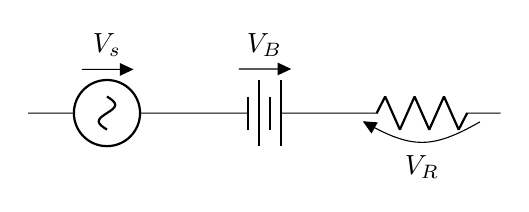
\begin{tikzpicture}[]
    \draw (0,0) to[sV, v=$V_s$] ++(2,0)
        to[battery, v=$V_B$] ++(2,0)
        to[R, v=$V_R$] ++(2,0);
\end{tikzpicture}
\end{LTXexample}

The consistency between symbols drawings and the default voltage and current directions are designed to work well \emph{when this default is enabled}. If you want, though, you can override this behavior by ``switching off'' the source status of the component by setting the property \texttt{bipole/is voltage} to \texttt{false}:

\begin{LTXexample}[varwidth=true, basicstyle=\small\ttfamily]
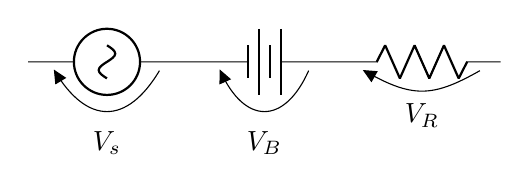
\begin{tikzpicture}[]
    \draw (0,0) to[sV, bipole/is voltage=false,
            v=$V_s$] ++(2,0)
        to[battery, bipole/is voltage=false,
            v=$V_B$] ++(2,0)
        to[R, v=$V_R$] ++(2,0);
\end{tikzpicture}
\end{LTXexample}

When you do this, \textbf{be careful} that (as you can see) the direction of the plain \texttt{v=...} option will change (please notice that this does not mean that it is incorrect, given that the voltage and current direction are arbitrary; in the case above, if the battery is a \SI{3}{V} one, $V_B=\SI{-3}{V}$ with the \texttt{RPvoltages} conventions).

Also, notice that there is an ordering problem in the \texttt{to[...]} options: you have to switch the \texttt{is voltage} property off \textbf{before} setting the voltage, otherwise you will have a mix of the source-type and passive positioning:

\begin{LTXexample}[varwidth=true, basicstyle=\small\ttfamily]
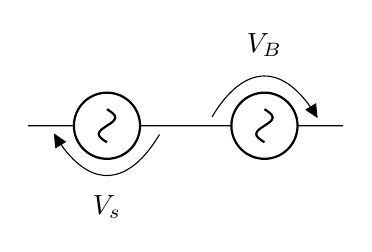
\begin{tikzpicture}[]
    % correct way
    \draw (0,0) to[sV, bipole/is voltage=false, v=$V_s$] ++(2,0)
    % wrong way, setting voltage before changing type
        to[sV=$V_B$ , bipole/is voltage=false, ] ++(2,0);
\end{tikzpicture}
\end{LTXexample}

In the first \texttt{to[]} command, the voltage is set before changing the type (assigning a value to the name of the element is understood as a \texttt{v=...} command for voltage sources).

A similar switch is present for current generators, called \texttt{bipoles/.is current}, acting in a very similar way.

If you would prefer to switch to the \texttt{is voltage=false, is current=false} behavior by default, you can (since \texttt{v1.4.4}\footnote{Suggested by user \href{https://github.com/circuitikz/circuitikz/issues/590}{\texttt{@judober} on GitHub}.}) by setting the option \texttt{bipole/override source vif} to \texttt{true}. This is \emph{highly} experimental, so use with care.

\begin{LTXexample}[varwidth=true, basicstyle=\small\ttfamily]
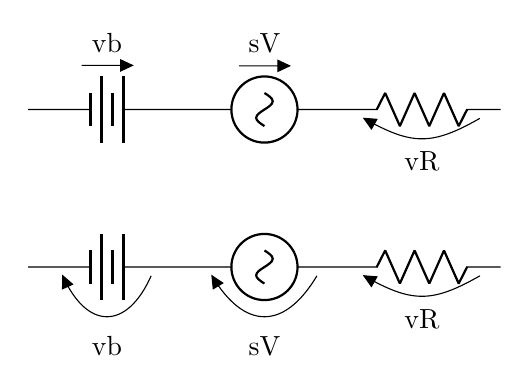
\begin{tikzpicture}[]
    \draw (0,0) to [battery=vb] ++(2,0)
        to[sV=sV] ++(2,0) to[R, v=vR] ++(2,0);
    \ctikzset{bipole/override source vif=true}
    \draw (0,-2) to [battery=vb] ++(2,0)
        to[sV=sV] ++(2,0) to[R, v=vR] ++(2,0);
\end{tikzpicture}
\end{LTXexample}

Notice that the option \texttt{override source vif} is ``stronger'' than the normal \texttt{is voltage}; so to locally re-set the behavior for just one source, you need to disable that \emph{before} using a voltage designator.

\begin{LTXexample}[varwidth=true, basicstyle=\small\ttfamily]
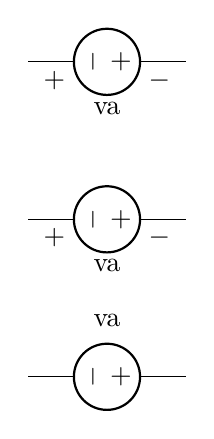
\begin{tikzpicture}[american]
    % dangerous option ahead: USE WITH CARE
    \ctikzset{bipole/override source vif=true}
    % ugly output, you should really use V>=va
    \draw (0,6) to [V=va] ++(2,0);
    % not working!
    \draw (0,4) to [V=va, bipole/override source vif=false] ++(2,0);
    % ok, this one is working --- you need both settings!
    \draw (0,2) to [V,
        bipole/override source vif=false,
        bipole/is voltage=true,
        v=va] ++(2,0);
\end{tikzpicture}
\end{LTXexample}

Clearly, if you find yourself using the last component often, it is better to define a style, which will save you a lot of typing and help readability:

\begin{LTXexample}[varwidth=true, basicstyle=\small\ttfamily]
\tikzset{myV/.style={V, bipole/override source vif=false,
    bipole/is voltage=true, v={#1}}}%
\begin{tikzpicture}[american]
    % dangerous option ahead: USE WITH CARE
    \ctikzset{bipole/override source vif=true}
    \draw (0,0) to [V>=va] ++(2,0);
    \draw (0,-2) to[myV=vb] ++(2,0);
\end{tikzpicture}
\end{LTXexample}

On the other way around, you could use styles to set \texttt{is voltage=false} only on the components you use and without using the global switch --- which is the recommended way of doing it.

\subsection{Currents}\label{sec:currents}

Inline (along the wire) currents are selected with \verb|i_>|, \verb|i^<|, \verb|i>_|, \verb|i>^|, and various combinations; the default position and direction is obtained with the simple key \verb|i=...|.

Basically, \verb|^| and \verb|_| control if the label is above or below the line (above and below \textbf{do} depend on the direction of the component path), and \verb|<| and \verb|>| the direction of the arrow; swapping them (from for example from \verb|i^>| to \verb|i>^|) will switch the side of the component where the symbol is drawn. See the following examples:


\begin{LTXexample}[varwidth=true]
\begin{circuitikz}
   \draw (0,0) to[R, i^>=$i_1$] (2,0);
\end{circuitikz}
\end{LTXexample}

\begin{LTXexample}[varwidth=true]
\begin{circuitikz}
   \draw (0,0) to[R, i_>=$i_1$] (2,0);
\end{circuitikz}
\end{LTXexample}

\begin{LTXexample}[varwidth=true]
\begin{circuitikz}
   \draw (0,0) to[R, i^<=$i_1$] (2,0);
\end{circuitikz}
\end{LTXexample}

\begin{LTXexample}[varwidth=true]
\begin{circuitikz}
   \draw (0,0) to[R, i_<=$i_1$] (2,0);
\end{circuitikz}
\end{LTXexample}

\begin{LTXexample}[varwidth=true]
\begin{circuitikz}
   \draw (0,0) to[R, i>^=$i_1$] (2,0);
\end{circuitikz}
\end{LTXexample}

\begin{LTXexample}[varwidth=true]
\begin{circuitikz}
   \draw (0,0) to[R, i>_=$i_1$] (2,0);
\end{circuitikz}
\end{LTXexample}

\begin{LTXexample}[varwidth=true]
\begin{circuitikz}
   \draw (0,0) to[R, i<^=$i_1$] (2,0);
\end{circuitikz}
\end{LTXexample}

\begin{LTXexample}[varwidth=true]
\begin{circuitikz}
   \draw (0,0) to[R, i<_=$i_1$] (2,0);
\end{circuitikz}
\end{LTXexample}

Also notice that the direction of the path is important:

\begin{LTXexample}[varwidth=true]
\begin{circuitikz}
   \draw (2,1) to[R, i<=$i_1$] (0,1);
   \draw (0,0) to[R, i<=$i_1$] (2,0);
\end{circuitikz}
\end{LTXexample}

Default directions can change if the component is active or passive,\footnote{This is better explained in section~\ref{sec:source-vif}} following the chosen global voltage direction strategy (see section~\ref{curr-and-volt}).

\begin{LTXexample}[varwidth=true]
\begin{circuitikz}
   \draw (0,0) to[V=10V, i_=$i_1$] (2,0);
\end{circuitikz}
\end{LTXexample}

\begin{LTXexample}[varwidth=true]
\begin{circuitikz}[voltage dir=EF]
   \draw (0,0) to[V=10V, i_=$i_1$] (2,0);
\end{circuitikz}
\end{LTXexample}

\begin{LTXexample}[varwidth=true]
\begin{circuitikz}[american]
   \draw (0,0) to[V=10V, i_=$i_1$] (2,0);
\end{circuitikz}
\end{LTXexample}

\begin{LTXexample}[varwidth=true]
\begin{circuitikz}[american]
   \draw (0,0) to[V=10V,invert, i_=$i_1$] (2,0);
\end{circuitikz}
\end{LTXexample}

Current generators with the direct label (the one obtained by, for example, \texttt{I = something}) will treat it as a current:

\begin{LTXexample}[varwidth=true]
\begin{circuitikz}
   \draw (0,0) to[I=$a_1$] (2,0);
\end{circuitikz}
\end{LTXexample}

If you use the option \texttt{americancurrent} or using the style \texttt{[american currents]}
you can change the style of current generators.

\begin{LTXexample}[varwidth=true]
\begin{circuitikz}[american currents]
   \draw (0,0) to[I=$a_1$] (2,0);
\end{circuitikz}
\end{LTXexample}


\subsection{Flows}\label{flows}

As an alternative for the current arrows, you can also use the following ``flows''. They can also be used to indicate thermal or power flows. The syntax is pretty the same as for currents.

\begin{LTXexample}[varwidth=true]
\begin{circuitikz}
   \draw (0,0) to[R, f=$i_1$] (3,0);
\end{circuitikz}
\end{LTXexample}

\begin{LTXexample}[varwidth=true]
\begin{circuitikz}
   \draw (0,0) to[R, f<=$i_1$] (3,0);
\end{circuitikz}
\end{LTXexample}

\begin{LTXexample}[varwidth=true]
\begin{circuitikz}
   \draw (0,0) to[R, f_=$i_1$] (3,0);
\end{circuitikz}
\end{LTXexample}

\begin{LTXexample}[varwidth=true]
\begin{circuitikz}
   \draw (0,0) to[R, f_>=$i_1$] (3,0);
\end{circuitikz}
\end{LTXexample}

\begin{LTXexample}[varwidth=true]
\begin{circuitikz}
   \draw (0,0) to[R, f<^=$i_1$] (3,0);
\end{circuitikz}
\end{LTXexample}

\begin{LTXexample}[varwidth=true]
\begin{circuitikz}
   \draw (0,0) to[R, f<_=$i_1$] (3,0);
\end{circuitikz}
\end{LTXexample}

\begin{LTXexample}[varwidth=true]
\begin{circuitikz}
   \draw (0,0) to[R, f>_=$i_1$] (3,0);
\end{circuitikz}
\end{LTXexample}

\subsection{Voltages}
See the introduction at Currents and Voltages (section~\ref{curr-and-volt}, page \pageref{curr-and-volt}) for the default direction of the voltage and currents.

Voltages come in four different styles: European (with curved or straight arrows) and American (with signs that can stay near the wire or raised at the label level).

Direction and position of the symbols are controlled in the same way as for the currents (see section~\ref{sec:currents}) with the \verb|_^<>| symbols.

\subsubsection{European style} The default, with curved arrows. Use option \texttt{europeanvoltage} or style \verb![european voltages]!, or setting (even locally) \texttt{voltage=european}.

\begin{LTXexample}[varwidth=true]
\begin{circuitikz}[european voltages]
   \draw (0,0) to[R, v^>=$v_1$] (2,0);
\end{circuitikz}
\end{LTXexample}

\begin{LTXexample}[varwidth=true]
\begin{circuitikz}[european voltages]
   \draw (0,0) to[R, v^<=$v_1$] (2,0);
\end{circuitikz}
\end{LTXexample}

\begin{LTXexample}[varwidth=true]
\begin{circuitikz}[european voltages]
   \draw (0,0) to[R, v_>=$v_1$] (2,0);
\end{circuitikz}
\end{LTXexample}

\begin{LTXexample}[varwidth=true]
\begin{circuitikz}[european voltages]
   \draw (0,0) to[R, v_<=$v_1$] (2,0);
\end{circuitikz}
\end{LTXexample}

The default direction for active elements can change, depending on the global \texttt{voltage dir} setting, so be careful.

\begin{LTXexample}[varwidth=true]
\begin{circuitikz}
   \draw (0,0) to[I=1A, v_=$u_1$] (2,0);
\end{circuitikz}
\end{LTXexample}

\begin{LTXexample}[varwidth=true]
\begin{circuitikz}
   \draw (0,0) to[I<=1A, v_=$u_1$] (2,0);
\end{circuitikz}
\end{LTXexample}

\begin{LTXexample}[varwidth=true]
\begin{circuitikz}
   \draw (0,0) to[I=$~$,l=1A, v_=$u_1$] (2,0);
\end{circuitikz}
\end{LTXexample}

\begin{LTXexample}[varwidth=true]
\begin{circuitikz}
   \draw (0,0) to[I,l=1A, v_=$u_1$] (2,0);
\end{circuitikz}
\end{LTXexample}

Moreover, for historical reasons, voltage generators have differently looking arrows (they are straight even in curved European style).
\begin{LTXexample}[varwidth=true]
\begin{circuitikz}
   \draw (0,0) to[battery,l_=1V, v=$u_1$, i=$i_1$] (2,0);
\end{circuitikz}
\end{LTXexample}

\begin{LTXexample}[varwidth=true]
\begin{circuitikz}
   \draw (0,0) to[V=10V, i_=$i_1$] (2,0);
\end{circuitikz}
\end{LTXexample}

You can change this last thing by forcing ``off'' the status of ``voltage generator''  of the component; but now the normal (passive) rule will apply, so, again, be careful and read section~\ref{sec:source-vif}.

\begin{LTXexample}[varwidth=true]
\begin{circuitikz}
   \draw (0,0) to[battery, bipole/is voltage=false,
                 v>=$u_1$,] (2,0);
\end{circuitikz}
\end{LTXexample}

As for the currents, the direct label of voltage sources is passed as a voltage:

\begin{LTXexample}[varwidth=true]
\begin{circuitikz}
   \draw (0,0) to[cV=$k\cdot a_1$] (2,0);
\end{circuitikz}
\end{LTXexample}

The following results from using the option \texttt{americanvoltage} or the style \texttt{[american voltages]}.

\begin{LTXexample}[varwidth=true]
\begin{circuitikz}[american voltages]
   \draw (0,0) to[V=$a_1$] (2,0);
\end{circuitikz}
\end{LTXexample}

\subsubsection{Straight European style} Using straight arrows. Use option \texttt{straightvoltages} or style \verb![straight voltages]!, or setting (even locally) \texttt{voltage=straight}.

\begin{LTXexample}[varwidth=true]
\begin{circuitikz}[straight voltages]
   \draw (0,0) to[R, v^>=$v_1$] (2,0);
\end{circuitikz}
\end{LTXexample}

\begin{LTXexample}[varwidth=true]
\begin{circuitikz}[straight voltages]
   \draw (0,0) to[R, v^<=$v_1$] (2,0);
\end{circuitikz}
\end{LTXexample}

\begin{LTXexample}[varwidth=true]
\begin{circuitikz}[straight voltages]
   \draw (0,0) to[R, v_>=$v_1$] (2,0);
\end{circuitikz}
\end{LTXexample}

\begin{LTXexample}[varwidth=true]
\begin{circuitikz}[straight voltages]
   \draw (0,0) to[R, v_<=$v_1$] (2,0);
\end{circuitikz}
\end{LTXexample}

Again, voltage generators are treated differently:

\begin{LTXexample}[varwidth=true]
\begin{circuitikz}[straight voltages]
   \draw (0,0) to[V=10V, i_=$i_1$] (3,0);
\end{circuitikz}
\end{LTXexample}

\begin{LTXexample}[varwidth=true]
\begin{circuitikz}[straight voltages]
   \draw (0,0) to[I, v=10V, i_=$i_1$] (3,0);
\end{circuitikz}
\end{LTXexample}

And you can override that with \texttt{bipole/is voltage} keeping into account that the default direction will be the one of passive components (see~\ref{sec:source-vif}):

\begin{LTXexample}[varwidth=true]
\begin{circuitikz}[straight voltages]
   \draw (0,0) to[V, bipole/is voltage=false,
        v=10V, i_=$i_1$] (3,0);
\end{circuitikz}
\end{LTXexample}

\subsubsection{American style}
Use option \texttt{americanvoltage} or set \verb![american voltages]! or use the option \texttt{voltage=american}.

\begin{LTXexample}[varwidth=true]
\begin{circuitikz}[american voltages]
   \draw (0,0) to[R, v^>=$v_1$] (2,0);
\end{circuitikz}
\end{LTXexample}

\begin{LTXexample}[varwidth=true]
\begin{circuitikz}[american voltages]
   \draw (0,0) to[R, v^<=$v_1$] (2,0);
\end{circuitikz}
\end{LTXexample}

\begin{LTXexample}[varwidth=true]
\begin{circuitikz}[american voltages]
   \draw (0,0) to[R, v_>=$v_1$] (2,0);
\end{circuitikz}
\end{LTXexample}

\begin{LTXexample}[varwidth=true]
\begin{circuitikz}[american voltages]
   \draw (0,0) to[R, v_<=$v_1$] (2,0);
\end{circuitikz}
\end{LTXexample}

\begin{LTXexample}[varwidth=true]
\begin{circuitikz}[american]
   \draw (0,0) to[I=1A, v_=$u_1$] (2,0);
\end{circuitikz}
\end{LTXexample}

\begin{LTXexample}[varwidth=true]
\begin{circuitikz}[american]
   \draw (0,0) to[I<=1A, v_=$i_1$] (2,0);
\end{circuitikz}
\end{LTXexample}


\subsubsection{Raised American style}

Since version \texttt{1.2.1}, ``raised'' American voltages are available; to use them, set the style \verb![raised voltages]! or use the option \texttt{voltage=raised}.
This is a version of the American-style voltage where the signs are raised to the level of the label.
The label is centered between the two signs, and the position of the signs is calculated by supposing that the label itself will be pretty simple; if you have very big labels you will need to adjust the position with \texttt{voltage shift} and/or the \texttt{voltage/distance from node} properties (see section~\ref{sec:common-vif-pos}).

\begin{LTXexample}[varwidth=true]
\begin{circuitikz}[raised voltages]
   \draw (0,0) to[R, v^>=$v_1$] (2,0);
\end{circuitikz}
\end{LTXexample}

\begin{LTXexample}[varwidth=true]
\begin{circuitikz}[raised voltages]
   \draw (0,0) to[R, v^<=$v_1$] (2,0);
\end{circuitikz}
\end{LTXexample}

\begin{LTXexample}[varwidth=true]
\begin{circuitikz}[raised voltages]
   \draw (0,0) to[R, v_>=$v_1$] (2,0);
\end{circuitikz}
\end{LTXexample}

\begin{LTXexample}[varwidth=true]
\begin{circuitikz}[raised voltages]
   \draw (0,0) to[R, v_<=$v_1$] (2,0);
\end{circuitikz}
\end{LTXexample}

\begin{LTXexample}[varwidth=true]
\begin{circuitikz}[american]
   \ctikzset{voltage=raised}
   \draw (0,0) to[I=1A, v_=$u_1$] (2,0);
\end{circuitikz}
\end{LTXexample}

\begin{LTXexample}[varwidth=true]
\begin{circuitikz}[raised voltages]
   \draw (0,0) to[I<=1A, v_=$i_1$] (2,0);
\end{circuitikz}
\end{LTXexample}

\subsubsection{Voltage position}\label{sec:sub-voltage-position}

It is possible to move the arrows and the plus or minus signs away from the component with the key \texttt{voltages shift} (default value is \texttt{0}, which gives the standard position):

\begin{LTXexample}[varwidth=true]
\begin{circuitikz}[]
   \draw (0,0) to[R, v=$v_1$, i=$i_1$] (2,0);
   \draw (0,-1) to[R, v=$v_1$, i=$i_1$,
      voltage shift=0.5] (2,-1);
   \draw (0,-2) to[R, v=$v_1$, i=$i_1$,
      voltage shift=1.0] (2,-2);
\end{circuitikz}
\end{LTXexample}

\begin{LTXexample}[varwidth=true]
\begin{circuitikz}[american voltages, voltage shift=0.5]
   \draw (0,0) to[R, v=$v_1$, i=$i_1$] (2,0);
\end{circuitikz}
\end{LTXexample}

Negative values do work as expected:

\begin{LTXexample}[varwidth=true]
\begin{circuitikz}[raised voltages]
   \draw (0,1.5) to[R, v^=$v_1$, i=$i_1$] ++(2,0);
   \draw (0,0) to[R, v^=$v_1$, i_=$i_1$,
        voltage shift=-1.0] ++(2,0);
\end{circuitikz}
\end{LTXexample}

You can fine-tune the position of the \texttt{+} and \texttt{-} symbols and the label in independent way using \texttt{voltage/shift} (default \texttt{0.0} for the former and \texttt{voltage/american label distance} (the distance of the label from the lines of the symbols, default \texttt{1.4}) for the latter.

\begin{LTXexample}[varwidth=true]
\begin{circuitikz}[american voltages]
    \draw (0,1) to[R, v=$v_1$, i=$i_1$] ++(2,0);
    % normally 1.4, make it tighter
    \ctikzset{voltage/american label distance=0.5}
    \draw (0,0) to[R, v=$v_1$, i=$i_1$] ++(2,0);
\end{circuitikz}
\end{LTXexample}

Notes that \texttt{american voltage} also affects batteries.

\begin{LTXexample}[varwidth=true]
\begin{circuitikz}[voltage shift=0.5]
   \draw (0,0) to[battery,l_=1V, v=$u_1$, i=$i_1$] (2,0);
\end{circuitikz}
\end{LTXexample}

\begin{LTXexample}[varwidth=true]
\begin{circuitikz}[american voltages, voltage shift=0.5]
   \draw (0,0) to[battery,l_=1V, v=$u_1$, i=$i_1$] (2,0);
\end{circuitikz}
\end{LTXexample}

Additionally, the \texttt{open} component is treated differently; the voltage is placed in the middle of the open space\footnote{Since \texttt{v1.1.2}, thank to an \href{https://github.com/circuitikz/circuitikz/issues/374}{issue opened by user \texttt{rhandley} on GitHub}.}:

\begin{LTXexample}[varwidth=true]
\begin{circuitikz}[american voltages]
    \draw (0,1.5) -- ++(0.5,0)
        to[open, v=$v_o$, o-o] ++(2,0) -- ++(0.5,0);
    \draw (0,0) -- ++(0.5,0)
        to[open, v=$v_o$, voltage=straight, *-*] ++(2,0)
        -- ++(0.5,0);
\end{circuitikz}
\end{LTXexample}

If you want or need to maintain the old behavior for \texttt{open} voltage, you can set the key \texttt{open voltage position} to \texttt{legacy} (the default is the new behavior, which corresponds to the value \texttt{center}).

\subsubsection{American voltages customization}\label{sec:american-voltage-custom}

Since 0.9.0, you can change the font\footnote{There was a bug before, noticed by the user \texttt{dzereb} on \href{https://tex.stackexchange.com/questions/487683/odd-minus-style-when-drawing-american-voltage}{tex.stackexchange.com} which made the symbols using different fonts in a basically random way. In the same page, user \texttt{campa} found the problem. Thanks!} used by the \texttt{american voltages} style, by setting to something different from nothing the key \texttt{voltage/american font} (default: nothing, using the current font) style:

\begin{LTXexample}[varwidth=true]
\begin{circuitikz}[american]
    \begin{scope}
        \ctikzset{voltage/american font=\tiny\boldmath}
        \draw (0,0) to[R,v=$V_S$] ++(2,0);
    \end{scope}
    \draw (0,-2) to[R,v=$V_S$] ++(2,0);
\end{circuitikz}
\end{LTXexample}

Also, if you want to change the symbols (sometimes just the $+$ sign is drawn, for example, or for highlighting something),
using the keys \texttt{voltage/american plus} and \texttt{voltage/american minus} (default \verb|$+$| and \verb|$\vphantom{+}-$|).

Notice that the definition of the minus sign is not simply \verb|$-$| because in most font (but not Computer Modern!) the size of the bounding box for the mathematical plus or minus are different. The \verb|\vphantom| forces the vertical size of the minus sign to be the same as the plus sign.\footnote{Changed in v1.6.3, you can look at \href{https://github.com/circuitikz/circuitikz/issues/721}{this issue on GitHub} for more details.}

\begin{LTXexample}[varwidth=true]
\begin{circuitikz}[american]
    \ctikzset{voltage/american font=\scriptsize\boldmath}
    \ctikzset{voltage/american plus=\textcolor{red}{$\oplus$}}
    \ctikzset{voltage/american minus=\textcolor{blue}{$\ominus$}}
    \draw (0,0) to[R,v_>=$V_S$] ++(2,0);
    \draw (0,-2) to[R,v_<=$V_S$] ++(2,0);
\end{circuitikz}
\end{LTXexample}

This could be especially useful if you define a style, to use like this:

\begin{LTXexample}[varwidth=true]
\tikzset{red plus/.style={
    circuitikz/voltage/american plus=\textcolor{red}{$+$},
}}
\begin{circuitikz}[american]
    \draw (0,0) to[R,v_>=$V_S$, red plus] ++(2,0);
    \draw (0,-2) to[R,v_<=$V_S$] ++(2,0);
\end{circuitikz}
\end{LTXexample}

\subsubsection{Combining different styles}\label{sec:mixing-voltage-styles}

Due to an historical hiccup, you need to be careful if you want to mix styles, like for example having \texttt{american} styled components and straight voltages (which are basically \texttt{european} style, at least in \Circuitikz{}). The problem is that the order of style parameters can change the output\footnote{%
thanks to Stack Exchange user \href{https://tex.stackexchange.com/q/665466/38080}{Mads P Olesen} for noticing.} as you can see in the following example, where in the red case the voltage generator shape reverted to the \texttt{european} one.

\begin{LTXexample}
\begin{circuitikz}[straight voltages, american]
    \draw (0,0) to [V, v=$V_P$] ++(0,3);
    \draw (1,0) to [R, v=$V_P$] ++(0,3);
\end{circuitikz}\color{red}%
\begin{circuitikz}[american, straight voltages]
    \draw (0,0) to [V, v=$V_P$] ++(0,3);
    \draw (1,0) to [R, v=$V_P$] ++(0,3);
\end{circuitikz}
\end{LTXexample}

This is arguably a bug, but fixing it (separating the voltage generator shapes from the voltage style) would break havoc with older circuits, so this will not be fixed for now.



\subsection{Changing the style of labels, voltages, and other text ornaments}\label{sec:ornament-style}

Since version \texttt{0.9.5}, it is possible to change the style of bipole text ornaments (labels, annotations, voltages etc) by using the appropriate styles or keys.
The basic style applied to the text is defined in the \texttt{/tikz/circuitikz} key directory and applied to every node that contains the text; you can also change them locally by using the \texttt{tikz} direct keys in local scopes.

For example, you can make all annotations small by using:

\begin{lstlisting}[numbers=none]
\ctikzset{bipole annotation style/.style={font=\small}}
\end{lstlisting}

And/or change (override) the setting in one specific bipole using:

\begin{lstlisting}[numbers=none]
...to[bipole annotation style={color=red}, R, a={Red note}]...
\end{lstlisting}

where the annotation will be in normal font (it has been reset!) and red, or append to the style:

\begin{lstlisting}[numbers=none]
...to[bipole annotation append style={color=red}, R, a={Red small note}]...
\end{lstlisting}

\textbf{Caveat:} you have to put the style changing key at the start of the \texttt{to} arguments to have any effect\footnote{No, I do not know why. Hints and fixes are welcome.}.

The available styles and commands are \texttt{bipole label style}, \texttt{bipole annotation style}, \texttt{bipole voltage style}, \texttt{bipole current style}, and \texttt{bipole flow style}. The following example shows a bit of everything.


\begin{LTXexample}[pos=t ]
\begin{circuitikz}[american]
    \ctikzset{bipole annotation style/.style={font=\tiny}}
    \ctikzset{bipole current style/.style={font=\small\sffamily}}
    \draw (0,0) to [bipole annotation append style={fill=yellow}, R=L1, a=A1] ++(3,0)
        to [bipole label style={fill=cyan}, R, l2_=L2 and 2L, a^=A2] ++(3,0);
    \draw (7,0) to [bipole voltage style={color=blue},
        bipole flow style={fill=green, outer sep=5pt},
        R=R1, v=V1, i=I1, f>^=F1] ++(3,0)
    to [bipole current append style={color=red}, R, v<=V2, i^=I2, f>^=F2] ++(3,0);
\end{circuitikz}
\end{LTXexample}

\subsection{Accessing labels text nodes}

Since 0.9.5, you can access all the labels nodes\footnote{The access to \texttt{label}s and \texttt{annotation}s was present before, but not documented.} using special node names. So, if you use \texttt{name} to give a name to the bipole node, you can also access the following nodes: \texttt{namelabel} (notice: no space nor any other symbol between \texttt{name} and \texttt{label}!), \texttt{nameannotation}, \texttt{namevoltage}, \texttt{namecurrent} and \texttt{nameflow}. Notice that the node names are available only if the bipole has an anchor or an annotation, of course.

\begin{LTXexample}[varwidth=true,
            pos=t
    ]
\newcommand{\marknode}[2][45]{%
    \node[circle, draw, red, inner sep=1pt,
    pin={[red, font=\tiny]#1:#2}] at (#2.center) {};
}
\begin{circuitikz}[ american]
    \draw (0,0) to [R=L1, a=A1, name=L1] ++(3,0)
    to [R, l2_=L2 and 2L, a^=A2, name=L2] ++(3,0);
    \marknode{L1} \marknode{L1label} \marknode[0]{L1annotation}
    \marknode{L2} \marknode[0]{L2label} \marknode{L2annotation}
    \draw[blue] (L2label.south west) rectangle (L2label.north east);
    \draw (6.1,0) to [R=R1, v=V1, i=I1, f>^=F1, name=R1] ++(3,0)
    to [R, v<=V2, i^=I2, f>^=F2, name=R2] ++(3,0);
    \marknode[0]{R1voltage} \marknode[0]{R2voltage} \marknode[90]{R1current}
    \marknode[90]{R2current} \marknode{R1flow} \marknode{R2flow}
\end{circuitikz}
\end{LTXexample}


If you want to have more access to the label positioning algorithm, since \texttt{1.2.5} you can access the label  rotation using the command \texttt{\textbackslash ctikzgetdirection\{\emph{nodename}\}} (where node name is for example \texttt{L1label} or \texttt{L2annotation}), and the anchor used for positioning the node as \texttt{\textbackslash ctikzgetanchor\{\emph{component label}\}\{\emph{type}\}}, where \emph{component label} is, for example, \texttt{L1} and type is either \texttt{label} or \texttt{annotation} (notice that the syntax is slightly different, for implementation reasons).
Those values are available only if the dipole declares a \texttt{l} or \texttt{a} keys; if you want them without any label you need to declare a blank one (like for example \texttt{l=\textasciitilde}).
The following example gives an idea of the values of those macros for the three types of label positioning strategies.

\begin{LTXexample}[varwidth=true, pos=t]
\newcommand{\marklabann}[3][45]{% [angle] {node label} {type: label or annotation}
\node[circle, draw, blue, inner sep=1pt,
pin={[draw, blue, font=\tiny, align=left]#1:{#2 \\ dir: \ctikzgetdirection{#2#3} \\
        anchor: \ctikzgetanchor{#2}{#3}}}] at (#2#3.\ctikzgetanchor{#2}{#3}) {};}
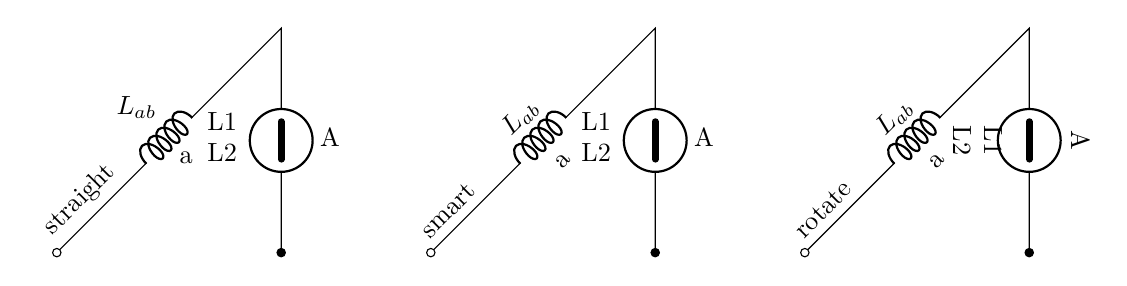
\begin{tikzpicture}[scale=0.95, transform shape]
\foreach \style/\xdelta in {straight/0, smart/5, rotate/10} {
\begin{scope}[xshift=\xdelta cm]
        \ctikzset{label/align = \style}
        \draw (0,0) node[above right, rotate=45]{\style}
            to[L, o-, l=$L_{ab}$, v, name=L1, a=a] ++(3,3)
            to[ceV, -*, v, name=V1, l2_=L1 and L2, a^=A] ++(0,-3);
        \marklabann[135]{L1}{label}
        \marklabann[-90]{L1}{annotation}
        \marklabann[90]{V1}{label}
        \marklabann[-90]{V1}{annotation}
\end{scope}}
\end{tikzpicture}
\end{LTXexample}



\subsection{Advanced voltages, currents and flows}\label{sec:vif-anchors}

Since version \texttt{1.2.1}\footnote{some options have been added in \texttt{v1.4.1}}, it is possible to access the anchors of the ``ornaments'' --- voltage, current and flows, together with some additional information that makes it possible to personalize them.
Normally, voltages and flow and currents are drawn into the path of the bipoles, so that it is not possible, for example, to change the line type or color of the arrows, or the type of arrows\footnote{in regular voltages, the arrows are not real \TikZ{} arrows, but the auxiliary arrow shapes of \Circuitikz{}}. Access to the anchors allows you to do all these things, and more.

For example, you can do something like this:

\begin{LTXexample}[varwidth=true]
\begin{circuitikz}[]
    \draw (0,1) to[R, v=$v$] ++(3,0);
    \draw (0,0) to[R, v, name=R, voltage/bump b=3] ++(3,0);
    \draw [thin, red, -{Stealth[width=8pt]}, ]
    (R-Vfrom) .. controls (R-Vcont1) and (R-Vcont2).. (R-Vto)
    node [black, pos=0.5, fill=white]{v};
\end{circuitikz}
\end{LTXexample}

Or, for example, to have a different voltage style; normally you would define a macro (see~\ref{sec:american-voltage-custom} to understand the \verb|\vphantom|).

\begin{LTXexample}[varwidth=true]
\begin{circuitikz}[voltage shift=0.5]
    \def\eurVPM#1#2{% node, label
        \draw [thin, -{Stealth[width=8pt]}, shorten >=5pt,
        shorten <=5pt] (#1-Vfrom) node[font=\tiny]{$\vphantom{+}-$}
        .. controls (#1-Vcont1) and (#1-Vcont2)..
        (#1-Vto) node[font=\tiny]{$+$}
        node[pos=0.5,anchor=\ctikzgetanchor{#1}{Vlab}]{#2};}
    \draw (0,0) to[R=R1, name=R1, v, i=$i$] ++(3,0)
        to[R, l_=R2, v^, name=R2] ++(0,-3);
    \eurVPM{R1}{$v_1$} \eurVPM{R2}{$v_2$}
\end{circuitikz}
\end{LTXexample}

Since \texttt{v1.4.1} you can also keep the voltage, current and flow labels and suppress the output of the symbols (arrows or plus/minus depending on the style) with the keys \texttt{no v symbols}, \texttt{no i symbols}, \texttt{no f symbols} (there are also the corresponding \texttt{v symbols}, \texttt{i symbols} and \texttt{f symbols} in case you want to switch the behavior off/on  globally). This for example simplify an often requested feature, like having all the current in one color and the voltages in another one, which is not possible natively because the arrows are part of the same path. One possible implementation of that is the following one:

\begin{LTXexample}[varwidth=true, basicstyle=\small\ttfamily]
\newcommand{\iarronly}[1]{% name
    \node [currarrow, color=red, anchor=center,
    rotate=\ctikzgetdirection{#1-Iarrow}] at (#1-Ipos) {};
}
\newcommand{\varronly}[1]{% name
    \draw [color=blue] (#1-Vfrom) .. controls (#1-Vcont1)
        and (#1-Vcont2)..  (#1-Vto) node [currarrow,
        sloped, anchor=tip, allow upside down,pos=1]{};
}
\begin{circuitikz}[]
    \ctikzset{!vi/.style={no v symbols, no i symbols}}
    \ctikzset{bipole voltage style/.style={color=blue},
        bipole current style/.style={color=red}}
    \draw (120:6) to[R, *-,  name=R, v^=$v_R$, !vi]
        (120:3) to[short, i=$i_R$, name=SR, !vi] (0,0);
    \draw (180:4) to[L, o-, l=$L$, name=L2, v=$v_L$, !vi]
        (180:2) to[V, -*, name=V2, v_=$v_2$, !vi] (0:0);
    \iarronly{SR}\varronly{R}\varronly{L2}\varronly{V2}
\end{circuitikz}
\end{LTXexample}

\subsubsection{Activating the anchors}

You will have access to the anchors for voltages, currents and flows when, in the bipole, you have both a \texttt{v}, \texttt{i}, \texttt{f} specification (one or more of them) \textbf{and} a \texttt{name} key, to give the bipole a name. Otherwise, the anchors and the associated functions are not defined.
To suppress the normal output of the \texttt{v}, \texttt{i}, \texttt{f} keys, you can use such keys without any argument, like in the previous example; notice that the \verb|_| and \verb|^| modifiers work as expected.

The following line of resistors has been drawn with the following commands; it is used to show the name of the available anchors.

\begin{lstlisting}
    \draw (0,0) to[R=R1, v=$v$, name=R1] ++(4,0)
        to[R, l_=R2, i=$i$, name=R2] ++(4,0)
        to[R=R3, f=$f$, name=R3] ++(4,0);
\end{lstlisting}

\begin{circuitikz}[]
    \draw (0,0) to[R=R1, v=$v$, name=R1] ++(4,0) to[R, l_=R2, i=$i$, name=R2] ++(4,0) to[R=R3, f=$f$, name=R3] ++(4,0);
    \path
    (R1-Vto) \showcoord(R1-Vto)<-135:0.2>
    (R1-Vfrom) \showcoord(R1-Vfrom)<-45:0.2>
    (R1-Vcont1) \showcoord(R1-Vcont1)<-45:0.2>
    (R1-Vcont2) \showcoord(R1-Vcont2)<-135:0.2>
    (R1-Vlab) \showcoord(R1-Vlab)<-90:0.5>
    (R2-Ito) \showcoord(R2-Ito)<45:0.3>
    (R2-Ifrom) \showcoord(R2-Ifrom)<135:0.3>
    (R2-Ipos) \showcoord(R2-Ipos)<-90:0.3>
    (R3-Fto) \showcoord(R3-Fto)<45:0.3>
    (R3-Ffrom) \showcoord(R3-Ffrom)<135:0.3>
    (R3-Fpos) \showcoord(R3-Fpos)<-90:0.4>
    ;
\end{circuitikz}

The meaning of the anchors is the following:
\begin{itemize}
\item
    \texttt{Vfrom} and \texttt{Vto} are the main points where the voltage information is given: start and end point of the arrow, or position of the $+$ or $-$ sign. This is the same for the \texttt{Ffrom} or \texttt{Fto} anchors for flows; for inline currents, the corresponding \texttt{Ifrom} and \texttt{Ito} mark the wire segment where the arrowhead is positioned (at the specified \texttt{current/distance} fraction. The direction of the arrow is available using the auxiliary macro \verb|\ctikzgetdirection| (see below).
\item
    \texttt{Vcont1} and \texttt{Vcont2} are the control points for the curved arrow (see the examples above); in the case of straight arrows or american-style voltages, they are set at the midpoint between \texttt{Vfrom} and \texttt{Vto}.
\item
    \texttt{Vlab} is where the text label for the voltage is normally positioned. The anchor used for such label is available using the auxiliary macro \verb|\ctikzgetanchor| (see below)
\item
    \texttt{Ipos} and \texttt{Fpos} are the position for the arrowhead or the small flow arrow (which is a \texttt{currarrow} or \texttt{flowarrow} node normally) is positioned, respectively. The label is then added to the correct side of it using the anchor available via \verb|\ctikzgetanchor| (see below,~\ref{sec:advances-aux-info}). In this case, the exact position of the label is not available if you do not position the element, for this there is no \texttt{Flab} or \texttt{Ilab} coordinate; you have to use the \texttt{Fpos} and \texttt{Ipos} coordinate with the corresponding \texttt{Ilab} and \texttt{Flab} anchors.
\end{itemize}

Changing the options of the elements will change the anchors accordingly:

\begin{lstlisting}
    \ctikzset{current/distance=0.2}
    \draw (0,0) to[R=R1, v>=$v$, name=R1] ++(4,0)
        to[R, l_=R2, i<_=$i$, name=R2] ++(4,0)
        to[R, l_=R3, f<_=$f$, name=R3] ++(4,0);
\end{lstlisting}

\begin{circuitikz}[]
    \ctikzset{current/distance=0.2}
    \draw (0,0) to[R=R1, v>=$v$, name=R1] ++(4,0) to[R, l_=R2, i<_=$i$, name=R2] ++(4,0) to[R, l_=R3, f<_=$f$, name=R3] ++(4,0);
    \path
    (R1-Vto) \showcoord(R1-Vto)<-45:0.2>
    (R1-Vfrom) \showcoord(R1-Vfrom)<-135:0.2>
    (R1-Vcont1) \showcoord(R1-Vcont1)<-135:0.2>
    (R1-Vcont2) \showcoord(R1-Vcont2)<-45:0.2>
    (R1-Vlab) \showcoord(R1-Vlab)<-90:0.5>
    (R2-Ito) \showcoord(R2-Ito)<135:0.3>
    (R2-Ifrom) \showcoord(R2-Ifrom)<45:0.3>
    (R2-Ipos) \showcoord(R2-Ipos)<90:0.3>
    (R3-Fto) \showcoord(R3-Fto)<90:0.4>
    (R3-Ffrom) \showcoord(R3-Ffrom)<80:0.4>
    (R3-Fpos) \showcoord(R3-Fpos)<-90:0.4>
    ;
\end{circuitikz}

Obviously, the anchors follow the voltage style you choose:

\begin{lstlisting}
    \draw (0,0) to[R=R1, v=$v$, name=R1, voltage=straight] ++(4,0)
        to[R=R2, v=$v$, name=R2, voltage=american] ++(4,0)
        to[R=R3, v=$v$, name=R3, voltage=raised] ++(4,0);
\end{lstlisting}

\begin{circuitikz}[]
    \ctikzset{current/distance=0.2}
    \draw (0,0) to[R=R1, v=$v$, name=R1, voltage=straight] ++(4,0)
        to[R=R2, v=$v$, name=R2, voltage=american] ++(4,0)
        to[R=R3, v=$v$, name=R3, voltage=raised] ++(4,0);
    \foreach \i in {1, 2, 3} {
        \path
        (R\i-Vto) \showcoord(R\i-Vto)<-90:0.4>
        (R\i-Vfrom) \showcoord(R\i-Vfrom)<-90:0.4>
        (R\i-Vcont1) \showcoord(R\i-Vcont1)<135:0.6>
        (R\i-Vcont2) \showcoord(R\i-Vcont2)<45:0.6>
        (R\i-Vlab) \showcoord(R\i-Vlab)<-90:0.6>
        ;
    }
\end{circuitikz}

Notice the position of the control points, as well as the fact that the anchor available with \verb|\ctikzgetanchor| is applied to \texttt{Vfrom} and \texttt{Vto} symbols, too.

Finally, as ever, generators are treated differently, but you have all your anchors too.

\begin{lstlisting}
    \ctikzset{american}
    \draw (0,0) to[V=$v$, name=G1, voltage=european] ++(4,0)
        to[V=$v$, v=$v$, name=G2, voltage=american] ++(4,0)
        to[battery2, v=$v$, name=G3, voltage=raised] ++(4,0);
\end{lstlisting}

\begin{circuitikz}[]
    \ctikzset{american}
    \draw (0,0) to[V=$v$, name=G1, voltage=european] ++(4,0)
        to[V=$v$, v=$v$, name=G2, voltage=american] ++(4,0)
        to[battery2, v=$v$, name=G3, voltage=raised] ++(4,0);
    \foreach \i in {1, 2, 3} {
        \path
        (G\i-Vto) \showcoord(G\i-Vto)<-60:0.1>
        (G\i-Vfrom) \showcoord(G\i-Vfrom)<-120:0.1>
        (G\i-Vlab) \showcoord(G\i-Vlab)<90:0.3>
        ;
    }
\end{circuitikz}

\subsubsection{Auxiliary information}\label{sec:advances-aux-info}

When the anchors are activated, there are additional macros that you can use:
\begin{itemize}
    \item \texttt{\textbackslash ctikzgetanchor\{\emph{<name>}\}\{\emph{<anchor>}\}}: \emph{name} is the name of the bipole, and \emph{anchor} can be \texttt{Vlab}, \texttt{Fpos} or \texttt{Ipos}. This macro expands to the normal anchor position (something like \texttt{north}, \texttt{south west}). Notice that if you have not activated the corresponding anchor, the content of this macro is not specified. It could be equivalent to \verb|\relax| (basically, empty) or contains the anchor of a bipole with the same name from another drawing --- it's a global macro like the coordinates.
    \item \texttt{\textbackslash ctikzgetdirection\{\emph{<name>}\}}: a number which is the direction of the \emph{name}d bipole.
    \item \texttt{\textbackslash ctikzgetdirection\{\emph{<name>}-Iarrow\}}: a number which is the direction of the current arrow requested for the \emph{name}d bipole; using \texttt{\emph{<name>}-Farrow} you get the same information for flow arrows.
\end{itemize}

For example, you could like the voltage label oriented with the bipole:

\begin{LTXexample}[varwidth=true]
\begin{circuitikz}[]
    \def\myvv#1#2{%
    \draw [thin, blue, ->,]
    (#1-Vfrom) .. controls (#1-Vcont1) and (#1-Vcont2).. (#1-Vto)
    node [pos=0.5, below,
    rotate=\ctikzgetdirection{#1}] at (#1-Vlab) {#2}; }
    \draw (0,0) to[R, v, name=A] ++(3,0);
    \draw (0,0) to[R, v, name=B] ++(3,3);
    \myvv{A}{$v_A$}\myvv{B}{$v_B$}
\end{circuitikz}
\end{LTXexample}

Or you could use the anchor to substitute the flow with a fancy one and still position the label automatically; suppose you have the following definition in your preamble (see \TikZ{} manual, ``Path decorations''):

\begin{lstlisting}
% requires \usetikzlibrary{decorations, decorations.pathmorphing}
\tikzset{%
lray/.style={decorate, decoration={
    snake, amplitude=2pt,pre length=1pt,post length=2pt, segment length=5pt,},
    -Triangle,
}}
\end{lstlisting}
\tikzset{%
lray/.style={decorate, decoration={
    snake, amplitude=2pt,pre length=1pt,post length=2pt, segment length=5pt, },
    -Triangle,
}}

You can then define a kind of ``power flow'' style:

\begin{LTXexample}[varwidth=true]
\begin{circuitikz}[]
    \newcommand\myff[3][blue]{% [opt: color] node label
        \draw [lray, #1, ] (#2-Ffrom) -- (#2-Fto)
        node [anchor=\ctikzgetanchor{#2}{Flab}, inner sep=4pt]
        at (#2-Fpos) {#3};}
    \draw (0,1) to[R, f, name=A] ++(3,0);
    \draw (0,0) to[R, f_<, name=B] ++(3,0);
    \myff{A}{$P_A$}\myff[red]{B}{$P_B$}
\end{circuitikz}
\end{LTXexample}



\subsubsection{Fixed voltage arrows: an example of advanced voltage usage}

\begingroup % to contain example definitions
An interesting application of the advanced voltage is to have fixed length straight voltage arrows.\footnote{This was suggested by users  \texttt{Franklin} and \texttt{Zarko} in \href{https://tex.stackexchange.com/questions/574576/circuitikz-straight-voltage-arrows-with-fixed-length}{a question on \texttt{tex.stackexchange.com}}}
The normal voltage arrows length depends not on the component length but on the node distance (this is the behavior since when the voltages were first introduced, so it can't be changed).

\begin{LTXexample}[varwidth=true, basicstyle=\scriptsize\ttfamily, pos=t]
\begin{circuitikz}[european,]
    \ctikzset{voltage=straight}
    \draw (0,0) to[R,v=$v_1$,*-*] ++(2,0) to[R, v<=$v_2$] ++(4,0) to[C, *-*, v=$v_3$] ++(1,0);
\end{circuitikz}
\end{LTXexample}

Using the advanced voltage interface mechanism, you can for example design voltages that are of fixed lengths; in the example below the new \texttt{xparse} method for defining commands is used, so that we can have a couple of different optional arguments:


\begin{lstlisting}[basicstyle=\scriptsize\ttfamily]
\NewDocumentCommand{\fixedvlen}{O{0.5cm} m m O{}}{% [semilength]{node}{label}[extra options]
    % get the center of the standard arrow
    \coordinate (#2-Vcenter) at ($(#2-Vfrom)!0.5!(#2-Vto)$);
    % draw an arrow of a fixed size around that center and on the same line
    \draw[-Triangle, #4] ($(#2-Vcenter)!#1!(#2-Vfrom)$) -- ($(#2-Vcenter)!#1!(#2-Vto)$);
    % position the label as in the normal voltages
    \node[anchor=\ctikzgetanchor{#2}{Vlab}, #4] at (#2-Vlab) {#3};
}
\end{lstlisting}
\NewDocumentCommand{\fixedvlen}{O{0.5cm} m m O{}}{% [semilength]{node}{label}[extra options]
    % get the center of the standard arrow
    \coordinate (#2-Vcenter) at ($(#2-Vfrom)!0.5!(#2-Vto)$);
    % draw an arrow of a fixed size around that center and on the same line
    \draw[-Triangle, #4] ($(#2-Vcenter)!#1!(#2-Vfrom)$) -- ($(#2-Vcenter)!#1!(#2-Vto)$);
    % position the label as in the normal voltages
    \node[anchor=\ctikzgetanchor{#2}{Vlab}, #4] at (#2-Vlab) {#3};
}

\begin{LTXexample}[varwidth=true, basicstyle=\scriptsize\ttfamily, pos=t]
\begin{circuitikz}[european,]
    \ctikzset{voltage=straight}
    \draw (0,2) to[R,v=$v_1$,*-*] ++(2,0) to[R, v<=$v_2$] ++(4,0) to[C, *-*, v=$v_3$] ++(1,0);
    \draw (0,0) to[R,v=,name=v1,*-*] ++(2,0) to[R, v<=, name=v2] ++(4,0) to[C, *-*, v, name=v3] ++(1,0);
    \fixedvlen{v1}{$V_1$}
    \fixedvlen{v2}{$V_2$}
    \fixedvlen{v3}{$V_3$}[red]
\end{circuitikz}
\end{LTXexample}

Notice that with a coherent naming you can use a \verb|\foreach| loop for the last three lines.

You can also notice that the arrow is not exactly the same as other arrows in the circuit; if you want them to be exactly the same, you can use a trick to get the default \Circuitikz{} arrow size --- please look at \href{https://tex.stackexchange.com/questions/549347/circuitikz-arrowhead/549354#549354}{this answer by Romano on \texttt{tex.stackexchange.com}}.

Another possibility is to have the arrow length based on the length of the component; for example you can use this code:

\begin{lstlisting}[basicstyle=\scriptsize\ttfamily]
\NewDocumentCommand{\compvlen}{O{1.5} m m O{}}{% [relative length]{node}{label}[extra options]
    % get the center of the standard arrow
    \coordinate (#2-Vcenter) at ($(#2-Vfrom)!0.5!(#2-Vto)$);
    % draw an arrow of a size proportional to the component length
    % around that center and on the same line
    % the component length is calculated using the let...in with the left and right anchors
    % and multiplied by the relative length
    \draw[-Triangle, #4] let \p1=(#2.left), \p2=(#2.right), \n1={0.5*#1*veclen(\x2-\x1,\y2-\y1)}
        in ($(#2-Vcenter)!\n1!(#2-Vfrom)$) -- ($(#2-Vcenter)!\n1!(#2-Vto)$);
    % position the label as in the normal voltages
    \node[anchor=\ctikzgetanchor{#2}{Vlab}, #4] at (#2-Vlab) {#3};
}
\end{lstlisting}
\NewDocumentCommand{\compvlen}{O{1.5} m m O{}}{% [relative length]{node}{label}[extra options]
    % get the center of the standard arrow
    \coordinate (#2-Vcenter) at ($(#2-Vfrom)!0.5!(#2-Vto)$);
    % draw an arrow of a size proportional to the component length
    % around that center and on the same line
    % the component length is calculated using the let...in with the left and right anchors
    % and multiplied by the relative length
    \draw[-Triangle, #4] let \p1=(#2.left), \p2=(#2.right), \n1={0.5*#1*veclen(\x2-\x1,\y2-\y1)}
        in ($(#2-Vcenter)!\n1!(#2-Vfrom)$) -- ($(#2-Vcenter)!\n1!(#2-Vto)$);
    % position the label as in the normal voltages
    \node[anchor=\ctikzgetanchor{#2}{Vlab}, #4] at (#2-Vlab) {#3};
}


\begin{LTXexample}[varwidth=true, basicstyle=\scriptsize\ttfamily, pos=t]
\begin{circuitikz}[european,]
    \ctikzset{voltage=straight}
    \draw (0,2) to[R,v=$v_1$,*-*] ++(2,0) to[R, v<=$v_2$] ++(4,0) to[C, *-*, v=$v_3$] ++(1,0);
    \draw (0,0) to[R,v=,name=v1,*-*] ++(2,0) to[R, v<=, name=v2] ++(4,0) to[C, *-*, v, name=v3] ++(1,0);
    \compvlen{v1}{$V_1$}
    \compvlen{v2}{$V_2$}
    \compvlen{v3}{$V_3$}[red]
\end{circuitikz}
\end{LTXexample}


\endgroup


\subsection{Integration with {\ttfamily siunitx}}

If the option {\ttfamily siunitx} is active\footnote{This option is still experimental --- personally (Romano) I would advise using the normal \texttt{\textbackslash SI\{\}\{\}} syntax, or the \texttt{\textbackslash qty\{\}\{\}} one for \texttt{siunitx} \texttt{v3} and newer.}, then the following are equivalent (this will \textbf{not} work in \ConTeXt{}, it has been disabled in upstream \ConTeXt, in favor of \href{https://www.pragma-ade.nl/general/manuals/units-mkiv.pdf}{its own \texttt{units} module}):

\begin{LTXexample}[varwidth=true]
\begin{circuitikz}
   \draw (0,0) to[R, l=1<\kilo\ohm>] (2,0);
\end{circuitikz}
\end{LTXexample}

\begin{LTXexample}[varwidth=true]
\begin{circuitikz}
   \draw (0,0) to[R, l=$\SI{1}{\kilo\ohm}$] (2,0);
\end{circuitikz}
\end{LTXexample}

\begin{LTXexample}[varwidth=true]
\begin{circuitikz}
   \draw (0,0) to[R, i=1<\milli\ampere>] (2,0);
\end{circuitikz}
\end{LTXexample}

\begin{LTXexample}[varwidth=true]
\begin{circuitikz}
   \draw (0,0) to[R, i=$\SI{1}{\milli\ampere}$] (2,0);
\end{circuitikz}
\end{LTXexample}

\begin{LTXexample}[varwidth=true]
\begin{circuitikz}
   \draw (0,0) to[R, v=1<\volt>] (2,0);
\end{circuitikz}
\end{LTXexample}

\begin{LTXexample}[varwidth=true]
\begin{circuitikz}
   \draw (0,0) to[R, v=$\SI{1}{\volt}$] (2,0);
\end{circuitikz}
\end{LTXexample}


\section{Using bipoles in circuits}

\subsection{Nodes (also called poles)}\label{sec:bipole-nodes}

You can add nodes to the bipoles, positioned at the coordinates surrounding the component. The general style to use is \texttt{bipole nodes=\{start\}\{stop\}}, where \texttt{start} and \texttt{stop} are the nodes --- to be chosen between \texttt{none}, \texttt{circ}, \texttt{ocirc}, \texttt{squarepole}, \texttt{osquarepole}, \texttt{diamondpole},  \texttt{odiamondpole} and \texttt{rectfill}\footnote{You can use other shapes too, but at your own risk\dots Moreover, notice that \texttt{none} is not really a node, just a special word used to say ``do not put any node here''.} (see section~\ref{sec:terminals}).


\begin{LTXexample}[varwidth=true,
        basicstyle=\small\ttfamily
    ]
\begin{circuitikz}
    \ctikzset{bipoles/length=.5cm, nodes width=0.1}%small components, big nodes
    \foreach \a/\p [evaluate=\a as \b using (\a+180)] in
    {-90/none, -60/circ, -30/ocirc, 0/diamondpole, 30/odiamondpole, 60/squarepole, 90/osquarepole}
        \draw (0,0) to[R, bipole nodes={none}{\p}] ++(\a:1.5)  node[font=\tiny, anchor=\b]{\p};
\end{circuitikz}
\end{LTXexample}

These bipole nodes are added \emph{after} any single path is drawn, as every node in \TikZ\ --- this is the reason why they are always filled (with the main color the normal nodes, with white the open ones), in order to ``hide'' the wire below. You can override the fill color if you want; but notice that if you draw things in two different paths, you will have ``strange'' results; notice that in the second line of resistors the second wire is starting from the center of the white \texttt{ocirc} of the previous path.

\begin{LTXexample}[varwidth=true,
        pos=t
    ]
\begin{circuitikz}
    \draw (0,0) to[R, *-o] ++(2,0) to[R, -d] ++(2,0)
        to[R, bipole nodes={diamondpole}{odiamondpole, fill=red}] ++(2,0);
    \draw (0,-1) to[R, *-o] ++(2,0) ;
    \draw (2,-1) to[R, -d] ++(2,0) to[R, bipole nodes={none}{squarepole}] ++(2,0);
\end{circuitikz}
\end{LTXexample}

You can define shortcuts for the \texttt{bipole nodes} you use most; for example if you want a shortcut for a bipole with open square node in red in the right side you can:

\begin{LTXexample}[varwidth=true,
        basicstyle=\small\ttfamily
    ]
\begin{circuitikz}
    \ctikzset{-s/.style = {bipole nodes={none}{osquarepole, fill=red}}}
    \draw (0,0) to[R, -s] ++(2,0);
\end{circuitikz}
\end{LTXexample}

There are several predefined shorthand as the above; in the following pages you can see all of them.

\begin{LTXexample}[varwidth=true]
\begin{circuitikz}
   \draw (0,0) to[R, o-o] (2,0);
\end{circuitikz}
\end{LTXexample}

\begin{LTXexample}[varwidth=true]
\begin{circuitikz}
   \draw (0,0) to[R, -o] (2,0);
\end{circuitikz}
\end{LTXexample}

\begin{LTXexample}[varwidth=true]
\begin{circuitikz}
   \draw (0,0) to[R, o-] (2,0);
\end{circuitikz}
\end{LTXexample}

\begin{LTXexample}[varwidth=true]
\begin{circuitikz}
   \draw (0,0) to[R, *-*] (2,0);
\end{circuitikz}
\end{LTXexample}

\begin{LTXexample}[varwidth=true]
\begin{circuitikz}
   \draw (0,0) to[R, -*] (2,0);
\end{circuitikz}
\end{LTXexample}

\begin{LTXexample}[varwidth=true]
\begin{circuitikz}
   \draw (0,0) to[R, *-] (2,0);
\end{circuitikz}
\end{LTXexample}

\begin{LTXexample}[varwidth=true]
\begin{circuitikz}
   \draw (0,0) to[R, d-d] (2,0);
\end{circuitikz}
\end{LTXexample}

\begin{LTXexample}[varwidth=true]
\begin{circuitikz}
   \draw (0,0) to[R, -d] (2,0);
\end{circuitikz}
\end{LTXexample}

\begin{LTXexample}[varwidth=true]
\begin{circuitikz}
   \draw (0,0) to[R, d-] (2,0);
\end{circuitikz}
\end{LTXexample}

\begin{LTXexample}[varwidth=true]
\begin{circuitikz}
   \draw (0,0) to[R, o-*] (2,0);
\end{circuitikz}
\end{LTXexample}

\begin{LTXexample}[varwidth=true]
\begin{circuitikz}
   \draw (0,0) to[R, *-o] (2,0);
\end{circuitikz}
\end{LTXexample}

\begin{LTXexample}[varwidth=true]
\begin{circuitikz}
   \draw (0,0) to[R, o-d] (2,0);
\end{circuitikz}
\end{LTXexample}

\begin{LTXexample}[varwidth=true]
\begin{circuitikz}
   \draw (0,0) to[R, d-o] (2,0);
\end{circuitikz}
\end{LTXexample}

\begin{LTXexample}[varwidth=true]
\begin{circuitikz}
   \draw (0,0) to[R, *-d] (2,0);
\end{circuitikz}
\end{LTXexample}

\begin{LTXexample}[varwidth=true]
\begin{circuitikz}
   \draw (0,0) to[R, d-*] (2,0);
\end{circuitikz}
\end{LTXexample}

\subsubsection{Transparent poles}\label{sec:transparent-poles}

``Open-poles'' terminals (\texttt{ocirc}, \texttt{odiamondpole}, and \texttt{osquarepole}) are normally filled with the background color at full opacity. The is reason is that \TikZ{}, when stroking a path, places and draws the nodes \emph{after} the lines are drawn; that way the poles ``white-out'' the underlying lines. Clearly this works if the wires and poles are written \emph{in the same path command}, otherwise the explicit order is respected.

Anyway, \emph{if you know what you are doing}, you can change it with the key \texttt{poles/open fill opacity} (with \verb|\ctikzset|) or the style \texttt{open poles opacity}. Notice that you will have artifacts if you don't use the border anchors of the poles to connect wires, and you need to do that by hand.

Notice that in poles, the opacity is \emph{always} selected with these keys, and it overrides the opacity of the draw commands (when not set explicitly is as if it is set to \texttt{1.0}, i.e., full opaque). This is because you normally do not want unfilled poles!

\begin{LTXexample}[pos=t]
\begin{circuitikz}[scale=3, transform shape]
    \fill[cyan] (0,0) rectangle (4.1,-0.6);
    \ctikzset{open poles fill=red}
    \tikzset{open poles opacity=0.5}
    % automatic positioning  when opacity is not 1.0 creates artifacts
    % note that the global fill opacity affects the "generic shape", but not the poles!
    % the fill color of the poles, instead, goes with the component
    \draw[fill opacity=0.8] (0,0) to[generic, fill=white, -o] ++(2,0) --++(0,-0.5);
    % \draw (0,0) to[generic, fill=white, -o] ++(2,0) --++(0,-0.5);
    % you have to use manual positioning
    \draw (2.2,0) -- ++(0.5,0) node[ocirc, anchor=180, fill opacity=0.5]{};
    \draw (3,0) node[ocirc, fill opacity=0.5](B){}  (B.0) --++(0.5,0) (B.-90) --++(0,-0.5);
    % maybe really useful only for terminals going out of the circuit...
    % notice that in node commands you can specify the opacity directly
    \draw (3.6,0) -- ++(0.2,0) node[ocirc, fill=white, fill opacity=0.5, anchor=180]{};
\end{circuitikz}
\end{LTXexample}

You also have the similar keys for the ``full'' poles (albeit they are probably not useful at all).


\subsection{Mirroring and Inverting}
Bipole paths can also be mirrored and inverted (or reverted) to change the drawing direction.

\begin{LTXexample}[varwidth=true]
\begin{circuitikz}
   \draw (0,0) to[pD] (2,0);
\end{circuitikz}
\end{LTXexample}

\begin{LTXexample}[varwidth=true]
\begin{circuitikz}
   \draw (0,0) to[pD, mirror] (2,0);
\end{circuitikz}
\end{LTXexample}
\begin{LTXexample}[varwidth=true]
\begin{circuitikz}
   \draw (0,0) to[pD, invert] (2,0);
\end{circuitikz}
\end{LTXexample}

Placing labels, currents and voltages also works, please note, that mirroring and inverting does not influence the positioning of labels and voltages. Labels are by default above/right of the bipole and voltages below/left, respectively.
\begin{LTXexample}[varwidth=true]
\begin{circuitikz}
   \draw (0,0) to[ospst=T, i=$i_1$, v=$v$] (2,0);
\end{circuitikz}
\end{LTXexample}

\begin{LTXexample}[varwidth=true]
\begin{circuitikz}
   \draw (0,0) to[ospst=T, mirror, i=$i_1$, v=$v$] (2,0);
\end{circuitikz}
\end{LTXexample}

\begin{LTXexample}[varwidth=true]
\begin{circuitikz}
   \draw (0,0) to[ospst=T, invert, i=$i_1$, v=$v$] (2,0);
\end{circuitikz}
\end{LTXexample}
\begin{LTXexample}[varwidth=true]
\begin{circuitikz}
   \draw (0,0) to[ospst=T,mirror,invert, i=$i_1$, v=$v$] (2,0);
\end{circuitikz}
\end{LTXexample}


\subsection{Putting them together}
\begin{LTXexample}[varwidth=true]
\begin{circuitikz}
   \draw (0,0) to[R=1<\kilo\ohm>,
      i>_=1<\milli\ampere>, o-*] (3,0);
\end{circuitikz}
\end{LTXexample}

\begin{LTXexample}[varwidth=true]
\begin{circuitikz}
   \draw (0,0) to[D*, v=$v_D$,
      i=1<\milli\ampere>, o-*] (3,0);
\end{circuitikz}
\end{LTXexample}

\subsection{Line joins between Path Components}
\label{sec:line-joins}

Line joins should be calculated correctly - if they are on the same path, and the path is not closed. For example, the following path is not closed correctly (\textit{--cycle} does not work here!):
\begin{LTXexample}[varwidth=true]
	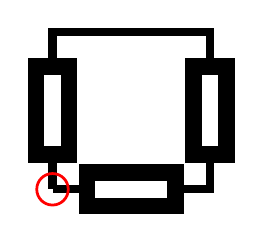
\begin{tikzpicture}[line width=3pt,european]
	\draw (0,0) to[R]++(2,0)to[R]++(0,2)
		--++(-2,0)to[R]++(0,-2);
	\draw[red,line width=1pt] circle(2mm);
	\end{tikzpicture}
\end{LTXexample}
To correct the line ending, there are support shapes to fill the missing rectangle. They can be used like the support shapes (*,o,d) using a dot (.) on one or both ends of a component (have a look at the last resistor in this example:
\begin{LTXexample}[varwidth=true]
	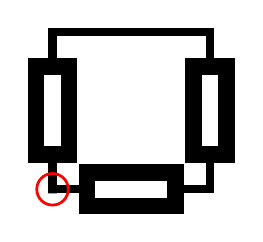
\begin{tikzpicture}[line width=3pt,european]
	\draw (0,0) to[R]++(2,0)to[R]++(0,2)
		--++(-2,0)to[R,-.]++(0,-2);
	\draw[red,line width=1pt] circle(2mm);
	\end{tikzpicture}
\end{LTXexample}

\section{Colors}\label{sec:colors}

Color support in \Circuitikz{} has been quite limited up to version 1.5.1; from that one onward there has been an effort to make components' behavior more intuitive.

Part of the problem is how colors in paths are treated by \TikZ{} itself; you can see part of the discussion on \href{https://github.com/circuitikz/circuitikz/issues/605}{this issue} and in \href{https://tex.stackexchange.com/questions/634987/pgf-basic-layer-struggling-again-with-colors}{this question on TeX.SX} --- many thanks to \texttt{@muzimuzhi} for helping there. Basically, nodes are drawn \emph{after} the path is completed, and color is applied to the path at the end. Look at this code (pure \TikZ, no \Circuitikz{} here):

\begin{LTXexample}[varwidth=true]
\tikz \draw[thick] (0,0) -- (1,0) {[color=red] -- (2,0) node[draw]{}} --(3,0); \par
\tikz \draw[thick] (0,0) -- (1,0) [color=red] -- (2,0) node[draw]{} --(3,0);
\end{LTXexample}

So the path is drawn with the last ``effective'' (in current group) color. The deferred behavior of the color properties is very difficult to track for \Circuitikz, especially when the shorthand \texttt{color-name} (e.g., \texttt{red} instead of \texttt{color=red}) is used. \Circuitikz{} will try to keep track of the colors specified by \texttt{color=...} and \texttt{fill=...}, but if you use the implicit way (\texttt{\textbackslash draw[red]...}) it often fails.

If you're adventurous, you can try to add
\begin{lstlisting}[numbers=none]
    \usepackage{regexpatch}\ctikzPatchImplicitColor
\end{lstlisting}
after loading \Circuitikz, and it will try to patch the default commands to keep track of the ``current color''; if it fails will give a warning like \texttt{patch failed, use only explicit color=...}. This is, unfortunately, not compatible with package \texttt{xpatch} (and much others, which load \texttt{xpatch}).\footnote{version \texttt{1.5.0} loaded it unconditionally for LaTeX; please do not use it}.

Before 1.5.0, \Circuitikz{} used black as the default color. Now it tries to follow the current color, as \TikZ{} does normally; but notice that there is a difference with the fill strategy:

\begin{LTXexample}[pos=t]
\color{red}
Red text
\tikz \draw (0,0) -- node[draw] {x} (1,0) -- node[draw=cyan] {y} (2,0);
\tikz \draw (0,0) to[R] (2,0) to[R,color=cyan] (4,0) to [generic] (6,0) to [fullgeneric] (8,0);

\color{blue}
Blue text
\tikz \draw (0,0) -- node[draw] {x} (1,0) -- node[draw=cyan] {y} (2,0);
\tikz \draw (0,0) to[R] (2,0) to[R,color=cyan] (4,0) to [generic] (6,0) to [fullgeneric] (8,0);

\color{black}
Black text
\tikz \draw[fill=yellow] (0,0) -- node[draw, fill] {x} (1,0) -- node[draw=cyan] {y} (2,0);
\tikz \draw[fill=yellow] (0,0) to[R] (2,0) to[R,color=cyan] (4,0) to [generic] (6,0) to [fullgeneric] (8,0);
\end{LTXexample}

\Circuitikz{} components that are fillable will inherit the \texttt{fill} property of the path (it is almost impossible to do otherwise) as if the \texttt{fill} flag was present. ``Full''-type elements (for example, full diodes or similar) are filled with the draw color; elements with intrinsic labels (i.e., labels that are part of the shape, like signs on amplifiers and pin numbers in chips) are drawn with the ``draw'' colors.

Basically, you should have no problem if:
\begin{enumerate}
    \item You stick to use styles (see~\ref{sec:styling-fillcolor}) for filling your components, or using a direct \texttt{fill=...} option in the component node or \texttt{to} option;
    \item do not try to change the color mid-path; sometimes it works (see the examples below), but it's better to avoid it (using different paths is better);
    \item when coloring whole circuits, it's better to use the option \texttt{color=...} in your global picture options or in the \verb|\draw| command (not just the color name as a shorthand);
    \item forget about transparency.
\end{enumerate}

Nevertheless, if you really need to do strange things with colors you can read on; you can do almost everything but there are several glitches to take into account.

\subsection{Shape colors}

The color of the components is stored in the key \verb!\circuitikzbasekey/color!. Circui\TikZ\ tries to follow the color set in \TikZ, although sometimes it fails. The following circuit will fail to draw the circuit in red if the patching of the inner commands of \TikZ{} fails, like for example in \ConTeXt{}.

\begin{LTXexample}[varwidth=true]
\begin{circuitikz} \draw[red]
  (0,2) node[and port](myand1){1}
  (0,0) node[and port](myand2){2}
  (2,1) node[xnor port](myxnor){3}
  (myand1.out) -| (myxnor.in 1)
  (myand2.out) -| (myxnor.in 2)
;\end{circuitikz}
\end{LTXexample}

If you see this problem, please do not use just the color name as a style, like \verb![red]!, but rather assign the style \verb![color=red]!.

\begin{LTXexample}[varwidth=true]
\begin{circuitikz} \draw[color=red]
  (0,2) node[and port](myand1){1}
  (0,0) node[and port](myand2){2}
  (2,1) node[xnor port](myxnor){3}
  (myand1.out) -| (myxnor.in 1)
  (myand2.out) -| (myxnor.in 2)
;\end{circuitikz}
\end{LTXexample}

One can, of course, change the color directly in the component:
\begin{LTXexample}[pos=t, varwidth=true]
\begin{circuitikz} \draw
  (0,0) node[pnp, color=blue](pnp2){q1}
  (pnp2.B) node[pnp, xscale=-1, anchor=B, color=brown](pnp1){\ctikzflipx{q2}}
  (pnp1.C) node[npn, anchor=C, color=green](npn1){q3}
  (pnp2.C) node[npn, xscale=-1, anchor=C, color=magenta](npn2){\ctikzflipx{q4}}
  (pnp1.E) -- (pnp2.E)  (npn1.E) -- (npn2.E)
  (pnp1.B) node[circ]{} |- (pnp2.C) node[circ]{}
;\end{circuitikz}
\end{LTXexample}

The all-in-one stream of bipoles poses some challenges, as only the actual body of the bipole, and not the connecting lines, will be rendered in the specified color (Notice that the following example uses the special \texttt{siunitx} shorthand; you can use it only in simple cases like here, in general using the full \verb|\SI{}| or \verb|\qty{}| commands).

\begin{LTXexample}[varwidth=true]
\begin{circuitikz} \draw
  (0,0) to[V=1<\volt>] (0,2)
        to[R=1<\ohm>, color=red] (2,2)
        to[C=1<\farad>] (2,0) -- (0,0)
;\end{circuitikz}
\end{LTXexample}

The postponed application of colors creates a problem if you want to use arrows for voltages, because the ``arrows'' are partially part of the path, partially nodes:

\begin{LTXexample}[varwidth=true]
\begin{circuitikz} \draw
  (0,0){[red] to[V=1<\volt>] (0,2) }
        to[R=1<\ohm>] (2,2)
        to[C=1<\farad>] (2,0) -- (0,0)
;\end{circuitikz}
\end{LTXexample}

...and that can become quite frustrating:

\begin{LTXexample}[varwidth=true]
\begin{circuitikz} \draw
  (0,0) to[V=1<\volt>, color=red] (0,2)
        to[R=1<\ohm>] (2,2)
        to[C=1<\farad>] (2,0) -- (0,0)
;\end{circuitikz}
\end{LTXexample}

In those cases, the only way out is to specify different paths (and/or using advanced voltages, see~\ref{sec:vif-anchors})

\begin{LTXexample}[varwidth=true]
\begin{circuitikz} \draw[color=red]
  (0,0) to[V=1<\volt>, color=red] (0,2);
  \draw (0,2) to[R=1<\ohm>] (2,2)
        to[C=1<\farad>] (2,0) -- (0,0)
;\end{circuitikz}
\end{LTXexample}

\subsection{Fill colors}

Since version 0.9.0, you can also fill most shapes with a color (the manual specifies which ones are fillable or not). The syntax is quite intuitive:

\begin{LTXexample}[varwidth=true]
\begin{circuitikz} \draw
    (0,2) node[and port, fill=yellow](myand1){1}
    (0,0) node[and port, fill=cyan](myand2){2}
    (2,1) node[xnor port,fill=red!30!white](myxnor){3}
  (myand1.out) -| (myxnor.in 1)
  (myand2.out) -| (myxnor.in 2)
;\end{circuitikz}
\end{LTXexample}


This fill color will override any color defined by the style (see section~\ref{sec:styling-fillcolor}). If you want to override a style fill color with no-fill for a specific component, you need to override the style --- it's a bit unfortunate, but should be an exceptional thing anyway. Notice that in simple case \texttt{fill opacity} works, but don't count too much on it.

\begin{LTXexample}[varwidth=true]
\begin{circuitikz}
    \ctikzset{logic ports/fill=cyan!30!white}
    \draw[red] (-0.5,3) -- (-0.5, -1);
    \draw[red] (1.5,3) -- (1.5, -1);
    \draw
    (0,2) node[and port](myand1){1}
    (0,0) node[and port, fill=cyan, fill opacity=0.7](myand2){2}
    (2,1) node[xnor port, circuitikz/logic ports/fill=none
              ](myxnor){3}
  (myand1.out) -| (myxnor.in 1)
  (myand2.out) -| (myxnor.in 2)
;\end{circuitikz}
\end{LTXexample}

You can combine shape colors with fill colors, too, but you should use the explicit \texttt{color} option style for this:

\begin{LTXexample}[varwidth=true]
\begin{circuitikz} \draw[color=red]
    (0,2) node[and port, fill=yellow](myand1) {1}
    (0,0) node[and port, fill=cyan] (myand2){2}
    (2,1) node[xnor port,fill=red!30!white](myxnor){3}
  (myand1.out) -| (myxnor.in 1)
  (myand2.out) -| (myxnor.in 2)
;\end{circuitikz}
\end{LTXexample}

\begin{LTXexample}[varwidth=true]
\begin{circuitikz} \draw
  (0,2) node[and port, color=black](myand1){1}
  (0,0) node[and port, color=blue, fill=cyan](myand2){2}
  (2,1) node[xnor port, color=red, fill=cyan](myxnor){3}
  (myand1.out) -| (myxnor.in 1)
  (myand2.out) -| (myxnor.in 2)
;\end{circuitikz}
\end{LTXexample}

\subsubsection{Background colors different from white}

Notice also that the connection point is always filled, and the color \emph{tries} to follow the color of the filling of the component (but look at section~\ref{sec:transparent-poles}). Moreover, if you want to pass fill transparency down to path-style components, you \emph{have} to put it into the options of the \verb|\draw| command.

\begin{LTXexample}[varwidth=true, pos=t]
\begin{circuitikz}
    \fill[cyan] (0,3.0) rectangle (7,7);
    \draw [fill opacity=0.5] (1,6.5) to[generic, fill=white,o-o] ++(2,0);
    \draw (1,5.5) to[short, fill=red, o-o] ++(1,0) to[short, -o] ++(1,0);
    \draw[fill=yellow] (1,5) to[short, o-o] ++(1,0) to[short, -o] ++(1,0);
    \draw (1,4.5) to[short, o-o] ++(1,0) to[short, -o] ++(1,0);
    \draw (1,4) node[ocirc]{} -- ++(1,0) node[ocirc]{};
    \draw [thick, color=green!50!black] (4,4) to [D,o-o,fill=yellow] ++(0,2) to[D*, fill=yellow]
        ++(2,0) to[D*,fill=yellow] ++(0,-2)  to[D, fill=red, o-o] ++(-2,0);
\end{circuitikz}
\end{LTXexample}

As you can see, the ``black'' components (as \texttt{D*}) follow the color of the line, not the fill.

Note, however, that if you choose a colored background, for example with the \verb|\pagecolor{}| command or with other tricks, the nodes will be by default still filled with white.

\begin{LTXexample}[varwidth=true]
\begin{circuitikz}[european]
    \fill[color=blue] (-1,-1) rectangle (4,1);
    \draw[color=white] (0,0) to[R, o-o] ++(3,0);
\end{circuitikz}
\end{LTXexample}

You have two solutions for this. You can redefine the \texttt{o-o} (and the similar commands \texttt{-o}, \texttt{o-}, \texttt{*-o} and so on) with a blue filled ``open'' pole:

\begin{LTXexample}[varwidth=true]
\tikzset{bcirc/.style={shape=ocirc, fill=blue}}
\ctikzset{o-o/.style ={
    \circuitikzbasekey/bipole/nodes/left=bcirc,
    \circuitikzbasekey/bipole/nodes/right=bcirc}}
\begin{circuitikz}[european]
    \fill[color=blue] (-1,-1) rectangle (4,1);
    \draw[color=white] (0,0) to[R, o-o] ++(3,0);
\end{circuitikz}
\end{LTXexample}

Also, since \texttt{v1.2.3}, you can set the key \texttt{open poles fill} (default: \texttt{white} which works for \texttt{ocirc}, \texttt{odiamondpole} and \texttt{osquarepole}):

\begin{LTXexample}[varwidth=true]
\begin{circuitikz}[european]
    \ctikzset{open poles fill=blue}
    \fill[color=blue] (-1,-1) rectangle (4,1);
    \draw[color=white] (0,0) to[R, o-o] ++(3,0);
\end{circuitikz}
\end{LTXexample}


\section{FAQ: Frequently asked questions}

\def\faqQ{\par\medskip\noindent\textbf{Q: }}
\def\faqA{\par\noindent\textbf{A: }}

\subsection{Using named nodes in circuits}\label{faqs:nodes}

\faqQ When I use a node to name a connection in the circuit, I have gaps in the wires! I am sure it used to work!

\faqA This is explained in~\ref{sec:incompatible-changes}. The fast answer is that in a hurry, use the \texttt{1.1.2} fallback point with:

\verb|\usepackage{circuitikz-1.1.2}|

in your preamble.

But really, your circuit definition is buggy, so the best thing to do is fix that; if you want to name a point in your circuit, you should use a \texttt{coordinate}, not a \texttt{node}.\footnote{Yes, I understand from where the confusion arise --- in circuit theory they are called nodes.} Here is a small tutorial on \emph{why} you should change your circuit.

Nodes, in \TikZ, normally have a non-zero size even when they are empty; moreover, connections are supposed to join the border of nodes. Please study the following (pure \TikZ, not \Circuitikz):

\begin{LTXexample}[varwidth=true]
\begin{tikzpicture}
    \path (1,1) node (A){}; % empty node at (1,1)
    \draw (1,0) -- (A) -- (2,1); % surprise!
\end{tikzpicture}
\end{LTXexample}

The gap is there because the node has a non-zero size (more in detail, its \texttt{inner sep} is by default different from zero). You can see it easily if you draw the node shape:

\begin{LTXexample}[varwidth=true]
\begin{tikzpicture}
    \path (1,1) node [draw=red](A){};
    \draw (1,0) -- (A) -- (2,1);
\end{tikzpicture}
\end{LTXexample}

The problem is that when you want to name a coordinate, in the sense of a dimensionless point, you should use a \texttt{coordinate}, \textbf{not} a node!

\begin{LTXexample}[varwidth=true]
\begin{tikzpicture}
    \path (1,1) coordinate (A); % give a name to (1,1)
    \draw (1,0) -- (A) -- (2,1);% now it's ok!
\end{tikzpicture}
\end{LTXexample}

Now, before version \texttt{1.2.1} (and since around \texttt{0.6}), \Circuitikz{} was detecting  when a connection was between nodes and sort-of added a \texttt{node.center} movement to the path. That in turn generated the need of hacks to draw the correct joining of lines, because that kind of movement broke the continuity of the path, like in this example:

\begin{LTXexample}[varwidth=true]
    
\begin{tikzpicture}[line width=4pt]
    \path (1,1) node (A){};
    \draw (1,0) -- (A.center) (A) (A.center) -- (2,1);
\end{tikzpicture}
\end{LTXexample}

You can see more examples and more reasonings on GitHub; start from the
\href{https://github.com/circuitikz/circuitikz/issues/417}{issue detecting the join problem}, then
\href{https://github.com/circuitikz/circuitikz/pull/418}{look at the merged fix}; you can follow several issues and discussions from there, but for example there are circuits that can't be drawn with the ``hack'' in, \href{https://github.com/circuitikz/circuitikz/issues/76#issuecomment-652980687}{like this one}.

So finally it was decided\footnote{well, Romano decided, so you can blame him. \emph{I do not think that workarounds to correct malformed circuits are really maintainable; just see the bunch of code removed by the patch! --- Romano.}}  to remove the change, to simplify the code and to make the package more maintainable.

\subsection{Using dashed (or colored) wires in circuits}\label{faqs:dashed}

\faqQ How can I make part of the wires dashed (or colored)? This does not work:

\begin{LTXexample}[varwidth=true]
\begin{circuitikz}
    \draw (0,0) to[R] ++(2,0)
    to[short, dashed, red] ++(1,0)
    to [R] ++(2,0); % surprise!
\end{circuitikz}
\end{LTXexample}

Nor this one, which is even stranger:

\begin{LTXexample}[varwidth=true]
\begin{circuitikz}
    \draw (0,0) to[R] ++(2,0)
    [dashed, red] -- ++(1,0)
    to [R] ++(2,0); % surprise!
\end{circuitikz}
\end{LTXexample}

\faqA This is an effect on how \TikZ{} builds and draws path. As explained in the \TikZ{} manual,\footnote{in 3.1.5b, section~14, ``syntax for path specification''} most path options are globally valid for the whole path; color and dash/dot is one of this. You have two options in this case. The first one is to use two paths.

\begin{LTXexample}[varwidth=true]
\begin{circuitikz}
    \draw (0,0) to[R] ++(2,0) coordinate(a);
    \draw [dashed, red] (a) -- ++(1,0) coordinate(b);
    \draw (b) to [R] ++(2,0);
\end{circuitikz}
\end{LTXexample}

The other one is to use \texttt{edge} operations\footnote{I took the idea form \href{https://tex.stackexchange.com/a/554905/38080}{this answer by \texttt{@LaTeXdraw-com} user on TeX.SE}, thanks!}; be sure to read about it on the \TikZ{} manual\footnote{in 3.1.5b, section~17.12, ``connecting nodes: use the \texttt{edge} operation''} --- but basically this is similar to the \texttt{to} operation but it builds another path (added at the end of the current path, like nodes are). This means that it can use different options, and that it \textbf{does not} move the path coordinates.

So, for example:

\begin{LTXexample}[varwidth=true]
\begin{circuitikz}
    \draw (0,0) to[R] ++(2,0)
    edge[dashed, red] ++(1,0)
    % we have to move the path position here!
    ++(1,0) to [R] ++(2,0);
\end{circuitikz}
\end{LTXexample}

The only problem with this approach is that the \texttt{edge}s are added \emph{after} the nodes, so it can create problems with nodes (look carefully!):

\begin{LTXexample}[varwidth=true]
\begin{circuitikz}
    \draw (0,0) to[R,-o] ++(2,0)
    edge[dashed, red] ++(1,0)
    ++(1,0) to [R] ++(2,0);
\end{circuitikz}
\end{LTXexample}

So it's better, in this case, to add the nodes manually after the path (there is no perfect solution!):

\begin{LTXexample}[varwidth=true]
\begin{circuitikz}
    \draw (0,0) to[R] ++(2,0) coordinate(a)
    edge[dashed, red] ++(1,0)
    ++(1,0) to [R] ++(2,0);
    \node [ocirc] at (a){};
\end{circuitikz}
\end{LTXexample}


A more complex example can be seen (look at the comments!) in the following circuit.

\begin{LTXexample}[varwidth=true]
\begin{circuitikz}[american]
    \draw (0,0) to[R, v=$v_1$] ++(2,0)
        edge[dashed] ++(1,0)
    ++(1,0) to[R]
    ++(2,0) to [R] ++(0,2) coordinate(a)
        edge[red, dashed] ++(0,1)
        % several edges start from the same position
        edge[dashed, ->] node[above]{here} ++(-1,0)
    % notice that the path here is still
    % at coordinate (a)!
    ++(0,1) to[R] ++(0,2)
    (a) ++(-1,0) to[sV] ++(-2,0);
\end{circuitikz}
\end{LTXexample}

\subsection{Errors when externalizing pictures}\label{faqs:externalize}

\faqQ When using \verb!\tikzexternalize! I get the following error:
\begin{verbatim}
 ! Emergency stop.
\end{verbatim}

\faqA The \TikZ\ manual states:

\begin{quotation}
\noindent Furthermore, the library assumes that all \LaTeX\ pictures are ended
    with \\\verb!\end{tikzpicture}!.
\end{quotation}

Just substitute every occurrence of the environment \verb!circuitikz! with \verb!tikzpicture!. They are actually pretty much the same.

\subsection{Labels, voltages and currents woes}\label{faqs:labels}

\faqQ How do I draw the voltage between two nodes?

\faqA Between any two nodes there is an open circuit!
\begin{LTXexample}[varwidth=true]
\begin{circuitikz} \draw
  node[ocirc] (A) at (0,0) {}
  node[ocirc] (B) at (2,1) {}
  (A) to[open, v=$v$] (B)
;\end{circuitikz}
\end{LTXexample}

\bigskip

\faqQ I cannot write \verb!to[R = $R_1=12V$]! nor \verb!to[ospst = open, 3s]!: I get errors.

\faqA It is a limitation of the parser, joined with a suboptimal processing by \Circuitikz{} (up to \texttt{1.2.7}) of the passing of the argument of keys.

You should protect commas and equal signs like in  \verb!to[R = {$R_1=12V$}]! or \verb!to[ospst = {open, 3s}]!.

In versions up to \texttt{1.2.7}, use for example \verb|\mbox{}| or define \verb|\def{\eq}{=}| and use \verb!to[R = $R_1\eq 12V$]!, or try to protect commas and equal signs like \verb!to[ospst = open{,} 3s]! or \verb|ospst=\mbox{open, 3s}| instead; see caveat in section~\ref{sec:labels-and-annotations}.

\subsection{Global scaling and rotating}\label{faqs:scale-and-rotate}

\faqQ I tried to change the direction of the $y$-axis with \texttt{yscale=-1}, but the circuit is completely messed up.

\faqA Yes, it's a known bug (or misfeature, or limitation). See section~\ref{sec:bugs}. Don't do that.


\faqQ I tried to put a diode in a \texttt{pic}, but it's coming out badly rotated.

\faqA Yes, it's a known bug (or misfeature, or limitation, or a fact of life). See section~\ref{sec:bugs}. \Circuitikz{} is not compatible with \texttt{pic}s at this point.

\subsection{Tunable components}\label{faq:tunable-arrow}

\faqQ The direction of the arrows in variable resistors or capacitors changed!

\faqA Yes, it changed in \texttt{v1.3.3}.

Version 1.3.3 fixes the direction of the arrows in tunable elements; before this version, they were more or less random, now the arrow goes from bottom left to top right. You have the option to go back to the old behavior with \texttt{\textbackslash ctikzset\{bipoles/fix tunable direction=false\}}. As a compensation for the fuss, now the arrows are configurable.


\begin{LTXexample}[pos=t]
\begin{circuitikz}[european]
    \draw (1,0) node{new default} (4,0) node{old default} (7,0) node{new!};
    \foreach [count=\i] \comp in
    {variable american resistor, variable european resistor,
        variable cute inductor, variable american inductor, tfullgeneric,
        variable capacitor} {
        \draw (0,-\i) node[left]{\texttt{\comp}} to[\comp, name=E] ++(2,0);
        \ctikzset{bipoles/fix tunable direction=false}
        \draw (3,-\i) to[\comp, name=E] ++(2,0);
        \ctikzset{bipoles/fix tunable direction=true, tunable end arrow={Bar}}
        \draw (6,-\i) to[\comp, name=E] ++(2,0);
    }
\end{circuitikz}
\end{LTXexample}


\section{Defining new components}

\begin{quote}
    Per me si va ne la città dolente,\\
    per me si va ne l'etterno dolore,\\
    per me si va tra la perduta gente.\\
    \dots\\
    Lasciate ogne speranza, voi ch'intrate.%
    \footnote{\url{https://classicsincontext.wordpress.com/2010/02/28/canto-iii-per-me-si-va-ne-la-citta-dolente/}}
\end{quote}


\textbf{Big fat warning}: this material is reserved for \TeX-hackers; do not delve into this if you have no familiarity with (at least) a bit of core \TeX{} programming and to the basic \TikZ{} layer. You have been warned.

\subsection{Suggested setup}

Notice: the source code has been reorganized after release 1.2.7; if you are bound to use an older version check the corresponding manual.

The suggested way to start working on a new component is to use the utilities of the \Circuitikz{} manual for checking and testing your device. Basically, find (or download) the source code of the last version of \Circuitikz{} and find the file \texttt{ctikzmanutils.sty}; copy it in your directory and prepare a file like this:

\begin{lstlisting}[keepspaces=true]
\documentclass[a4paper, titlepage]{article}
\usepackage{a4wide}         %smaller borders
\usepackage[utf8]{inputenc} %not needed since LaTeX 2019
\usepackage[T1]{fontenc}
\parindent=0pt
\parskip=4pt plus 6pt minus 2pt
\usepackage[siunitx, RPvoltages]{circuitikzgit}
\usepackage{ctikzmanutils}
\makeatletter
%%  Test things here
% defines

% components

% paths
\makeatother

\begin{document}

\circuitdescbip*{damper}{Mechanical damping}{}(left/135/0.2, right/45/0.2, center/-90/0.3)

\geolrcoord{dampershape, fill=yellow}

\begin{LTXexample}[varwidth]
\begin{circuitikz}
    \draw (0,0) to[R] ++(2,0)
    to[damper] ++(2,0);
\end{circuitikz}
\end{LTXexample}
\end{document}
\end{lstlisting}

This will compile to something like this (in this case, we are using a couple of existing components to check everything is OK):

\circuitdescbip*{damper}{Mechanical damping}{}(left/135/0.2, right/45/0.2, center/-90/0.3)

\geolrcoord{dampershape, fill=yellow}

\begin{LTXexample}[varwidth]
\begin{circuitikz}
    \draw (0,0) to[R] ++(2,0)
    to[damper] ++(2,0);
\end{circuitikz}
\end{LTXexample}

The command \verb|circuitdescbip*| is used to show the component description (you can check the definition and the usage looking at \texttt{ctikzmanutils.sty} file, and the \verb|\geolrcoord| is used to show the main anchors (geographical plus \texttt{left} and \texttt{right}) of the component.

From now on, you can add the new commands for the component between the \verb|\makeatletter| and \verb|\makeatother| commands and, modifying the example, check the results.

\subsection{Path-style component}

Let's define for example a path style component, like the one suggested by the user \texttt{@alex} on \href{https://tex.stackexchange.com/questions/484268/combined-spring-damper-in-circuitikz}{\TeX{} stackexchange site}. The component will be a mix of the \texttt{damper} and the \texttt{spring} components already present.

The definitions of the components are in the files \texttt{pgfcirc\emph{something}.tex}; they are more or less distributed by the number of terminals, but there are exceptions (for example, switches are in \texttt{bipoles}, even if several of them are tripoles or more\dots \texttt{grep} is your friend here.

To define the new component we will look into (in this case) \texttt{pgfcircbipoles.tex}; at the start of the block where the components are defined, you can find the relevant definitions (sometime some of the definitions are in \texttt{pgfcirc.defines.tex}, for historical or dependencies reasons).
The first step is to check if we can use the definition already existing for similar elements (for coherence of size) or if we need to define new ones; for this you have to check into the  we find

\begin{lstlisting}
    \ctikzset{bipoles/spring/height/.initial=.5}
    \ctikzset{bipoles/spring/width/.initial=.5}
    \ctikzset{bipoles/damper/height/.initial=.35}
    \ctikzset{bipoles/damper/length/.initial=.3}
    \ctikzset{bipoles/damper/width/.initial=.4}
\end{lstlisting}

We will use them; at this stage you can decide to add other parameters if you need them. (Notice, however, than although flexibility is good, these parameters should be described in the manual, otherwise they're as good as a fixed number in the code).


After that we will copy, for example, the definition of the damper into our code, just changing the name:

\begin{lstlisting}[keepspaces=true]
%% mechanical resistor - damper
\pgfcircdeclarebipolescaled{mechanicals}
{}                                   % extra anchors
{\ctikzvalof{bipoles/damper/height}} % depth (under the path line)
{viscoe}                             % name
{\ctikzvalof{bipoles/damper/height}} % height (above the path line)
{\ctikzvalof{bipoles/damper/width}}  % width
{
    \pgfpathrectanglecorners{\pgfpoint{\ctikzvalof{bipoles/damper/length}\pgf@circ@res@right}{\pgf@circ@res@down}}{\pgfpoint{\pgf@circ@res@right}{\pgf@circ@res@up}}
    \pgf@circ@maybefill

    % line into the damper
    \pgfpathmoveto{\pgfpoint{\pgf@circ@res@left}{\pgf@circ@res@zero}}
    \pgfpathlineto{\pgfpoint{\ctikzvalof{bipoles/damper/length}\pgf@circ@res@right}
        {\pgf@circ@res@zero}}
    \pgfusepath{stroke}

    % damper box
    \pgf@circ@setlinewidth{bipoles}{\pgfstartlinewidth}
    \pgfpathmoveto{\pgfpoint{\pgf@circ@res@left}{\pgf@circ@res@down}}
    \pgfpathlineto{\pgfpoint{\pgf@circ@res@right}{\pgf@circ@res@down}}
    \pgfpathlineto{\pgfpoint{\pgf@circ@res@right}{\pgf@circ@res@up}}
    \pgfpathlineto{\pgfpoint{\pgf@circ@res@left}{\pgf@circ@res@up}}

    \pgfsetrectcap
    \pgfsetmiterjoin
    \pgfusepath{stroke}

    % damper vertical element
    \pgfpathmoveto{\pgfpoint{\ctikzvalof{bipoles/damper/length}\pgf@circ@res@right}
        {.8\pgf@circ@res@down}}
    \pgfpathlineto{\pgfpoint{\ctikzvalof{bipoles/damper/length}\pgf@circ@res@right}
        {.8\pgf@circ@res@up}}
    \pgfsetbuttcap
    \pgfusepath{stroke}

}
\end{lstlisting}

This \verb|\pgfcircdeclarebipolescaled| command will define a shape that is named \texttt{viscoeshape}, with all the correct geographical anchors based on the depth, height and width defined in the parameters: in this case we are reusing the ones of the \texttt{damper} shape. Moreover, the element is assigned to the class \texttt{mechanicals} for styling.

To be coherent with the styling, you should use (when needed) the length \verb|\pgf@circ@scaled@Rlen| as the ``basic'' length for drawing, using the fill functions (they are defined at the start of the file \texttt{pgfcirc.defines.tex}) to fill and stroke --- so that the operation will follow the style parameters and, finally, use the macro \verb|\pgf@circ@setlinewidth| to set the line thickness: the first argument is the ``legacy'' class, if you do not want to assign one you can use the pseudo-legacy class \texttt{none}.

The anchors for the bipole (which then set the lengths \verb|\pgf@circ@res@left|) are already scaled for your use. You can use these lengths (which defines, normally, the geographical anchors of the element) to draw your shapes.

This is not sufficient for using the element in a \texttt{to[]} path command; you need to ``activate'' it (the definition of the commands are normally in \texttt{pgfcircpath.tex}). In this case the component is simple --- look at the definitions if you need to do more complex things.

\begin{lstlisting}
\pgfcirc@activate@bipole@simple{l}{viscoe}
\end{lstlisting}

In the definition above, the \texttt{\{l\}} parameter means that using the component like \texttt{to[viscoe=A]} will be equivalent to \texttt{to[viscoe, l=A]}; you can also use \texttt{v} or \texttt{i} or \texttt{f} if your component needs it.
Now you can show it with:

\begin{lstlisting}
\circuitdescbip*{viscoe}{Mechanical viscoelastic element}{}(left/135/0.2, right/45/0.2, center/-90/0.3)

\geolrcoord{viscoeshape, fill=yellow}

\begin{LTXexample}[varwidth]
\begin{circuitikz}
    \draw (0,0) to[spring] ++(2,0)
    to[viscoe] ++(2,0);
\end{circuitikz}
\end{LTXexample}
\end{lstlisting}

Obviously, at first you just have a component that is the same as the one you copied with another name.
It is now just a matter of modifying it so that it has the desired shape; in the example above you can already see the new symbol after the changes.

When doing the drawing in the main argument of the \verb|\pgfcircdeclarebipole|, things will be set up so that the lengths \verb|\pgf@circ@res@right|
and \verb|\pgf@circ@res@up| are the $x$-$y$ coordinates of the upper right corner, and
\verb|\pgf@circ@res@left|  and \verb|\pgf@circ@res@down| are the $x$-$y$ coordinates of the lower left corner of your shape. The \texttt{center} coordinate is usually at $(0pt, 0pt)$.

Looking at the implementation of the \texttt{spring} element, one possibility is changing the lines between  lines~12 and~16 with:

\begin{lstlisting}
    % spring into the damper
    \pgfscope
        \pgfpathmoveto{\pgfpoint{\pgf@circ@res@left}{\pgf@circ@res@zero}}
        \pgf@circ@setlinewidth{bipoles}{\pgfstartlinewidth}
        \pgfsetcornersarced{\pgfpoint{.25\pgf@circ@res@up}{.25\pgf@circ@res@up}}
        \pgfpathlineto{\pgfpoint{.75\pgf@circ@res@left}{.75\pgf@circ@res@up}}
        \pgfpathlineto{\pgfpoint{.5\pgf@circ@res@left}{-.75\pgf@circ@res@up}}
        \pgfpathlineto{\pgfpoint{.25\pgf@circ@res@left}{.75\pgf@circ@res@up}}
        \pgfpathlineto{\pgfpoint{0pt}{-.75\pgf@circ@res@up}}
        \pgfpathlineto{\pgfpoint{\ctikzvalof{bipoles/damper/length}\pgf@circ@res@right}{.75\pgf@circ@res@up}}
        \pgfusepath{stroke}
    \endpgfscope
\end{lstlisting}

which leads to:

\circuitdescbip*{viscoe}{Mechanical viscoelastic element}{}(left/135/0.2, right/45/0.2, center/-90/0.3)

\geolrcoord{viscoeshape, fill=yellow}

\begin{LTXexample}[varwidth]
\begin{circuitikz}
    \draw (0,0) to[spring] ++(2,0)
    to[viscoe] ++(2,0);
\end{circuitikz}
\end{LTXexample}

Now you can check if the voltage labels are correct for your new component:

\begin{LTXexample}[varwidth]
\begin{circuitikz}[]
    \draw (0,0) to[spring] ++(2,0)
    to[viscoe, v=V] ++(2,0);
\end{circuitikz}
\end{LTXexample}

If you think they are too tight or too loose, you can use a (developer-only) key to adjust the distance:

\begin{LTXexample}[varwidth]
\begin{circuitikz}
    \ctikzset{bipoles/viscoe/voltage/additional shift/.initial=1}
    \draw (0,0) to[spring] ++(2,0)
    to[viscoe, v=V] ++(2,0);
\end{circuitikz}
\end{LTXexample}

Notice that by default the key \texttt{bipoles/\emph{mybipole}/voltage/additional shift} is not defined, so if you want to use it you must create it before (this is the meaning of the \texttt{.initial} here).

Now you can save all the code between the \verb|\makeatletter| and \verb|\makeatother| in a file and \verb|\input{}| it for using your special component, or submit the component to the project (see below).

As a final note, notice that the \texttt{viscoe} element is already added to the standard package.

\subsection{Node-style component}

Adding a node-style component is much more straightforward. Just define it by following examples in, for example, \texttt{pgfcirctripoles.tex} or the other files; be careful that you should define all the geographical anchors of the shape if you want that the \TikZ{} positioning options (like \texttt{left}, \texttt{above}, etc.) behave correctly with your component.

To have a scalable component, for example in the \texttt{transistors} class, you should use something like
\begin{lstlisting}
        \savedmacro{\ctikzclass}{\edef\ctikzclass{transistors}}
        \saveddimen{\scaledRlen}{\pgfmathsetlength{\pgf@x}{\ctikzvalof{\ctikzclass/scale}\pgf@circ@Rlen}}
\end{lstlisting}
at the start of anchors and macros definition, and use (for example, the exact code will change greatly depending on your component):
\begin{lstlisting}
        \savedanchor\northeast{% upper right
            \pgfmathsetlength{\pgf@circ@scaled@Rlen}{\ctikzvalof{\ctikzclass/scale}\pgf@circ@Rlen}
            \pgf@y=\pgf@circ@scaled@Rlen
            \pgf@y=0.5\pgf@y
            \pgf@x=0.3\pgf@y
        }
\end{lstlisting}
in all the \texttt{savedanchors}.

Then, to draw your component, you should start with\footnote{Since \texttt{v1.5.0}; component defined with this mechanism will not be compatible with older \Circuitikz{}.}:
\begin{lstlisting}
    \pgf@circ@draw@component{%
        \pgf@circ@scaled@Rlen=\scaledRlen
        ...
    }
\end{lstlisting}
and then use \verb|\pgf@circ@scaled@Rlen| (or the anchors) as the default length while you draw it.

The special command \verb|\pgf@circ@draw@component| will issue a \texttt{\textbackslash behindforegroundpath} command, and take care of calling the start and end hooks for the component. Notice that, given the use of \texttt{\textbackslash behindforegroundpath}, you must take care to use the path you define here! The path itself is protected bu a \texttt{pgfscope} (and so also by a \TeX{} group), so local definitions will be reset after exiting.

\subsubsection{The internal hook system}\label{sec:drawing-hooks}

Since version \texttt{v1.5.0}, before starting the drawing of any component, \Circuitikz{} will check for the existence of three different hooks, in the following order (suppose that the shape name is \texttt{\emph{myname}}, and it has a class \texttt{\emph{myclass}}:
\begin{itemize}
    \item \texttt{\textbackslash ctikz@hook@start@draw@component@\emph{myname}}
    \item \texttt{\textbackslash ctikz@hook@start@draw@class@\emph{myclass}}
    \item \texttt{\textbackslash ctikz@hook@start@draw@default}
\end{itemize}
The first one that is defined in the current (or outer) scope is used, and the following ones are not used. These hooks can be used to set drawing parameters, or to reset them to a known state: \TikZ{} normally inherit most of the drawing option, but that can lead to surprises (like unexpected arrows, etc.).

In the same way, before leaving  \verb|\pgf@circ@draw@component|, a set of similar hooks (with \texttt{end} instead of \texttt{start}) is tried, with the same logic.

The only predefined hook is \texttt{\textbackslash ctikz@hook@start@draw@default}, which is set to the equivalent of:
\begin{lstlisting}
    \pgfsetshortenstart{+0pt}\pgfsetshortenend{+0pt}\pgfsetarrows{-}%
    \def\pgf@circ@reset@rounded{\pgfsetcornersarced{\pgfpointorigin}}%
\end{lstlisting}
which means that, by  default, arrows parameters are reset to the default (no shorten, no arrows) and that corners are not rounded. If you want to override them, just define the appropriate hook for your component/class and the generic one will not be called.

No \texttt{...@end@draw@...} hook is defined by default.

\subsubsection{Finishing your work}

Once you have a satisfactory element, you should
\begin{itemize}
    \item Clean up your code;
    \item write a piece of documentation explaining its use, with an example;
    \item Propose the element for inclusion in the GitHub page of the project (you will have to license this as explained in that page, of course).
\end{itemize}

The best way of contributing is forking the project, adding your component in the correct files, modifying the manual and creating a pull request for the developers to merge.  Anyway, if this is a problem, just open an issue and someone (when they have time\dots) will answer.

\section{Examples}

Here a series of examples, contributed by several people, is shown with their code.

\subsection{A red diode}

\begin{LTXexample}[pos=t,varwidth=true]
\begin{circuitikz}[scale=1.4]\draw
  (0,0) to[C, l=10<\micro\farad>] (0,2) -- (0,3)
        to[R, l=2.2<\kilo\ohm>] (4,3) -- (4,2)
        to[L, l=12<\milli\henry>, i=$i_1$,v=b] (4,0) -- (0,0)
  (4,2) to[D*, color=red] (2,0)
  (0,2) to[R, l=1<\kilo\ohm>, *-] (2,2)
        to[cV, i=1, -*, v=$\SI{.3}{\kilo\ohm}\, i_1$] (4,2)
  (2,0) to[I, i=1<\milli\ampere>, *-*] (2,2)
;\end{circuitikz}
\end{LTXexample}

\newpage
\subsection{Using the (experimental) \texttt{siunitx} syntax}

\begin{LTXexample}[pos=t,varwidth=true]
\begin{circuitikz}[scale=1.2]\draw
  (0,0) node[ground] {}
        to[V=$e(t)$, *-*] (0,2) to[C=4<\nano\farad>] (2,2)
        to[R, l_=.25<\kilo\ohm>, *-*] (2,0)
  (2,2) to[R=1<\kilo\ohm>] (4,2)
        to[C, l_=2<\nano\farad>, *-*] (4,0)
  (5,0) to[I, i_=$a(t)$, -*] (5,2) -- (4,2)
  (0,0) -- (5,0)
  (0,2) -- (0,3) to[L, l=2<\milli\henry>] (5,3) -- (5,2)

 {[anchor=south east] (0,2) node {1} (2,2) node {2} (4,2) node {3}}
;
\end{circuitikz}
\end{LTXexample}


\begin{LTXexample}[pos=t,varwidth=true]
\begin{circuitikz}[scale=1.2]\draw
  (0,0) node[anchor=east] {B}
        to[short, o-*] (1,0)
        to[R=20<\ohm>, *-*] (1,2)
        to[R=10<\ohm>, v=$v_x$] (3,2) -- (4,2)
        to[cI=$\frac{\si{\siemens}}{5} v_x$, *-*] (4,0) -- (3,0)
        to[R=5<\ohm>, *-*] (3,2)
  (3,0) -- (1,0)
  (1,2) to[short, -o] (0,2) node[anchor=east]{A}
;\end{circuitikz}
\end{LTXexample}

\newpage
\subsection{Photodiodes}

\begin{LTXexample}[pos=t,varwidth=true]
\begin{circuitikz}[scale=1]\draw
	(0,0) node[transformer] (T) {}
	(T.B2) to[pD] ($(T.B2)+(2,0)$) -| (3.5, -1)
	(T.B1) to[pD] ($(T.B1)+(2,0)$)  -| (3.5, -1)
;\end{circuitikz}
\end{LTXexample}

\subsection{A Sallen-Key cell}

\begin{LTXexample}[pos=t,varwidth=true]
\begin{circuitikz}[scale=1]\draw
    (5,.5) node [op amp] (opamp) {}
    (0,0) node [left] {$U_{we}$} to [R, l=$R_d$, o-*] (2,0)
    to [R, l=$R_d$, *-*] (opamp.+)
    to [C, l_=$C_{d2}$, *-] ($(opamp.+)+(0,-2)$) node [ground] {}
    (opamp.out) |- (3.5,2) to [C, l_=$C_{d1}$, *-] (2,2) to [short] (2,0)
    (opamp.-) -| (3.5,2)
    (opamp.out) to [short, *-o] (7,.5) node [right] {$U_{wy}$}
;\end{circuitikz}
\end{LTXexample}

\newpage
\subsection{Mixing circuits and graphs}

\begin{LTXexample}[pos=t,varwidth=true]
\begin{circuitikz}[scale=1.2, american]\draw
  (0,2) to[I=1<\milli\ampere>] (2,2)
        to[R, l_=2<\kilo\ohm>, *-*] (0,0)
        to[R, l_=2<\kilo\ohm>] (2,0)
        to[V, v_=2<\volt>] (2,2)
        to[cspst, l=$t_0$] (4,2) -- (4,1.5)
        to [generic, i=$i_1$, v=$v_1$] (4,-.5) -- (4,-1.5)
  (0,2) -- (0,-1.5) to[V, v_=4<\volt>] (2,-1.5)
        to [R, l=1<\kilo\ohm>] (4,-1.5);

   \begin{scope}[xshift=6.5cm, yshift=.5cm]
       \draw [->] (-2,0) -- (2.5,0) node[anchor=west] {$v_1/\si{\volt}$};
    \draw [->] (0,-2) -- (0,2) node[anchor=west] {$i_1/\si{\milli\ampere}$} ;
    \draw (-1,0) node[anchor=north] {-2} (1,0) node[anchor=south] {2}
          (0,1) node[anchor=west] {4} (0,-1) node[anchor=east] {-4}
          (2,0) node[anchor=north west] {4}
          (-1.5,0) node[anchor=south east] {-3};
    \draw [thick] (-2,-1) -- (-1,1) -- (1,-1) -- (2,0) -- (2.5,.5);
    \draw [dotted] (-1,1) -- (-1,0) (1,-1) -- (1,0)
          (-1,1) -- (0,1) (1,-1) -- (0,-1);
   \end{scope}
\end{circuitikz}
\end{LTXexample}

\newpage
\subsection{RF circuit}

\begin{LTXexample}[pos=t,varwidth=true]
    \begin{circuitikz}[scale=1]
        \ctikzset{bipoles/detector/width=.35}
        \ctikzset{quadpoles/coupler/width=1}
        \ctikzset{quadpoles/coupler/height=1}
        \ctikzset{tripoles/wilkinson/width=1}
        \ctikzset{tripoles/wilkinson/height=1}
        %\draw[help lines,red,thin,dotted] (0,-5) grid (5,5);
        \draw
        (-2,0) node[wilkinson](w1){}
        (2,0) node[coupler] (c1) {}
        (0,2) node[coupler,rotate=90] (c2) {}
        (0,-2) node[coupler,rotate=90] (c3) {}
        (w1.out1) .. controls ++(0.8,0) and ++(0,0.8) .. (c3.port3)
        (w1.out2) .. controls ++(0.8,0) and ++(0,-0.8) .. (c2.port4)
        (c1.port1) .. controls ++(-0.8,0) and ++(0,0.8) .. (c3.port2)
        (c1.port4) .. controls ++(-0.8,0) and ++(0,-0.8) .. (c2.port1)
        (w1.in) to[short,-o] ++(-1,0)
        (w1.in) node[left=30] {LO}
        (c1.port2) node[match,yscale=1] {}
        (c1.port3) to[short,-o] ++(1,0)
        (c1.port3) node[right=30] {RF}
        (c2.port3) to[detector,-o] ++(0,1.5)
        (c2.port2) to[detector,-o] ++(0,1.5)
        (c3.port1) to[detector,-o] ++(0,-1.5)
        (c3.port4) to[detector,-o] ++(0,-1.5)
        ;
    \end{circuitikz}
\end{LTXexample}

\subsection{A styled low noise input stage}

\ctikzloadstyle{romano}
\scalebox{0.707}{%
\begin{circuitikz}[american, romano circuit style]
    \ctikzset{bipoles/cuteswitch/thickness=0.5}
    \draw (0,0) node[ground](GND0){} to[sV, l=$v_{cm}$] ++(0,1)
    to [R, l=$R_c$, -*] ++(0,1.5) coordinate(vcm) --++(0,0.5) coordinate(diffc);
    \draw (diffc) -| ++(-0.5, 0.5) to[sV,l=$v_+$, name=vplus] ++(0,1) --++(0,2)
    -- ++(2.5,0) coordinate(skin+ a) to[battery2, l=$E_+$, name=eplus] ++(1,0)
    to[R=$R_+$, name=rplus] ++(2,0) coordinate(skin+ b) -- ++(0.5,0)
    -- ++(4,0) coordinate(hpin+) to[highpass] ++(2,0)
    node[inst amp, anchor=+, noinv input up,
    circuitikz/amplifiers/scale=1.6,
    circuitikz/tripoles/inst amp/width=1](LNA){LNA}
    (LNA.out);
    \coordinate (skin- a) at (LNA.- -| skin+ a);
    \draw (diffc) -| ++(0.5,0.5) to[sV,l_=$v_-$, name=vminus] ++(0, 1) |- (skin- a);
    \draw (skin- a) to[battery2, l_=$E_-$, name=eminus] ++(1,0)
    to[R, l_=$R_-$, name=rminus] ++(2,0) coordinate(skin- b) -- ++(2.5,0)
    -- (skin- b -| hpin+) to[highpass] (LNA.-);
    \coordinate (gnd a) at (vcm -| skin+ a);
    \draw (vcm) -- (gnd a) to[battery2, l_=$E_\mathrm{gnd}$, name=egnd] ++(1,0)
    to[R, l_=$R_\mathrm{gnd}$, name=rgnd] ++(2,0) coordinate(gnd b);
    % switch set
    \def\swdown{-3.2}
    \draw (skin- b) ++(1,0) coordinate(sw1) to[cosw, invert, mirror, l=1, *-, name=s1] ++(0,\swdown) to[short, -*] ++(0, -1.5);
    \draw (sw1) ++(1,0) coordinate(sw2) to[cosw, invert, mirror, l=2, *-] ++(0,\swdown) to[R=$R$, -*] ++(0, -1.5);
    \draw (sw2|-skin+ b) ++(1,0) coordinate(sw3) to[short, *-] (sw3|-sw2) to[cosw, invert, mirror, l=3,] ++(0,\swdown) to[R=$R$, -*] ++(0, -1.5);
    \draw (sw3) ++(1,0) coordinate(sw4) to[short, *-] (sw4|-sw2) to[cosw, invert, mirror, l=4, name=s4] ++(0,\swdown) to[short] ++(0, -1.5) coordinate(endsw);
    \draw (gnd b) |- (endsw) node[rectjoinfill]{};
    % boxes
    \node [rectangle, draw, dashed, fit=(GND0) (vplus) (vpluslabel) (vminuslabel)](body){};
    \node [anchor=south east, align=center] at (body.south east) {Body} ;
    \node [rectangle, draw, dashed, fit=(rplus) (eplus) (epluslabel) (rpluslabel)](top){};
    \node [rectangle, draw, dashed, fit=(eminus) (rminus) (eminuslabel) (rminuslabel)](bot){};
    \node [anchor=center, align=center] at ($(top.south)!0.5!(bot.north)$) {electrodes} ;
    \node [rectangle, draw, dashed, fit=(egnd) (rgnd) (egndlabel) (rgndlabel)](gnd){};
    \node [below, align=center] at (gnd.south) {ground\\ electrode} ;
    \node [rectangle, draw, dashed, fit=(s1) (s4label), inner ysep=8pt](switches){};
    % ADC and micro
    \draw (LNA.out) -- ++(0.5,0) node[msport,circuitikz/RF/scale=2](ADC){ADC};
    \draw (ADC.right) -- ++(0.5,0) node[twoportshape, anchor=left, t=$\upmu$C](uC){};
    \draw (uC.south) -- (uC.south |- switches.east) -- ++(-4,0)
    node[align=left, anchor=east](DCS){\small digitally\\ controlled\\ switches};
    \draw[-Stealth] (DCS.west) -- (switches.east);
    % components
    \node [anchor=north west] at ([xshift=-10pt, yshift=-5pt]switches.south east) {ADG1414};
    \node [anchor=north west] at ([yshift=-5pt]LNA.refv down) {AD8429};
\end{circuitikz}
} % scalebox

\begin{lstlisting}[basicstyle=\small\ttfamily]
\ctikzloadstyle{romano}
\scalebox{0.707}{%
\begin{circuitikz}[american, romano circuit style]
    \ctikzset{bipoles/cuteswitch/thickness=0.5}
    \draw (0,0) node[ground](GND0){} to[sV, l=$v_{cm}$] ++(0,1)
    to [R, l=$R_c$, -*] ++(0,1.5) coordinate(vcm) --++(0,0.5) coordinate(diffc);
    \draw (diffc) -| ++(-0.5, 0.5) to[sV,l=$v_+$, name=vplus] ++(0,1) --++(0,2)
    -- ++(2.5,0) coordinate(skin+ a) to[battery2, l=$E_+$, name=eplus] ++(1,0)
    to[R=$R_+$, name=rplus] ++(2,0) coordinate(skin+ b) -- ++(0.5,0)
    -- ++(4,0) coordinate(hpin+) to[highpass] ++(2,0)
    node[inst amp, anchor=+, noinv input up,
    circuitikz/amplifiers/scale=1.6,
    circuitikz/tripoles/inst amp/width=1](LNA){LNA}
    (LNA.out);
    \coordinate (skin- a) at (LNA.- -| skin+ a);
    \draw (diffc) -| ++(0.5,0.5) to[sV,l_=$v_-$, name=vminus] ++(0, 1) |- (skin- a);
    \draw (skin- a) to[battery2, l_=$E_-$, name=eminus] ++(1,0)
    to[R, l_=$R_-$, name=rminus] ++(2,0) coordinate(skin- b) -- ++(2.5,0)
    -- (skin- b -| hpin+) to[highpass] (LNA.-);
    \coordinate (gnd a) at (vcm -| skin+ a);
    \draw (vcm) -- (gnd a) to[battery2, l_=$E_\mathrm{gnd}$, name=egnd] ++(1,0)
    to[R, l_=$R_\mathrm{gnd}$, name=rgnd] ++(2,0) coordinate(gnd b);
    % switch set
    \def\swdown{-3.2}
    \draw (skin- b) ++(1,0) coordinate(sw1) to[cosw, invert, mirror, l=1, *-, name=s1] ++(0,\swdown) to[short, -*] ++(0, -1.5);
    \draw (sw1) ++(1,0) coordinate(sw2) to[cosw, invert, mirror, l=2, *-] ++(0,\swdown) to[R=$R$, -*] ++(0, -1.5);
    \draw (sw2|-skin+ b) ++(1,0) coordinate(sw3) to[short, *-] (sw3|-sw2) to[cosw, invert, mirror, l=3,] ++(0,\swdown) to[R=$R$, -*] ++(0, -1.5);
    \draw (sw3) ++(1,0) coordinate(sw4) to[short, *-] (sw4|-sw2) to[cosw, invert, mirror, l=4, name=s4] ++(0,\swdown) to[short] ++(0, -1.5) coordinate(endsw);
    \draw (gnd b) |- (endsw) node[rectjoinfill]{};
    % boxes
    \node [rectangle, draw, dashed, fit=(GND0) (vplus) (vpluslabel) (vminuslabel)](body){};
    \node [anchor=south east, align=center] at (body.south east) {Body} ;
    \node [rectangle, draw, dashed, fit=(rplus) (eplus) (epluslabel) (rpluslabel)](top){};
    \node [rectangle, draw, dashed, fit=(eminus) (rminus) (eminuslabel) (rminuslabel)](bot){};
    \node [anchor=center, align=center] at ($(top.south)!0.5!(bot.north)$) {electrodes} ;
    \node [rectangle, draw, dashed, fit=(egnd) (rgnd) (egndlabel) (rgndlabel)](gnd){};
    \node [below, align=center] at (gnd.south) {ground\\ electrode} ;
    \node [rectangle, draw, dashed, fit=(s1) (s4label), inner ysep=8pt](switches){};
    % ADC and micro
    \draw (LNA.out) -- ++(0.5,0) node[msport,circuitikz/RF/scale=2](ADC){ADC};
    \draw (ADC.right) -- ++(0.5,0) node[twoportshape, anchor=left, t=$\upmu$C](uC){};
    \draw (uC.south) -- (uC.south |- switches.east) -- ++(-4,0)
    node[align=left, anchor=east](DCS){\small digitally\\ controlled\\ switches};
    \draw[-Stealth] (DCS.west) -- (switches.east);
    % components
    \node [anchor=north west] at ([xshift=-10pt, yshift=-5pt]switches.south east) {ADG1414};
    \node [anchor=north west] at ([yshift=-5pt]LNA.refv down) {AD8429};
\end{circuitikz}
} % scalebox
\end{lstlisting}

\subsection{An example with the \texttt{compatibility} option}
\label{ex:compatibility}

\IfFileExists{compatibility.pdf}{\fbox{\includegraphics{compatibility.pdf}}}{}%

\begin{lstlisting}
\documentclass{standalone}

\usepackage{tikz}
\usetikzlibrary{circuits.ee.IEC}
\usetikzlibrary{positioning}

\usepackage[compatibility]{circuitikzgit}
\ctikzset{bipoles/length=.9cm}

\begin{document}
 \begin{tikzpicture}[circuit ee IEC]
  \draw (0,0) to [resistor={name=R}] (0,2)
	to[diode={name=D}] (3,2);
  \draw (0,0) to[*R=$R_1$] (1.5,0) to[*Tnpn] (3,0)
    to[*D](3,2);
 \end{tikzpicture}
\end{document}
\end{lstlisting}

\newpage
\subsection{3-phases block schematic}

\begin{LTXexample}[varwidth=true,pos=t]
\begin{circuitikz}[smallR/.style={european resistor, resistors/scale=0.5}]
    \draw (0,0) node[tacdcshape, anchor=ac mid in](acdc){} to[smallR] ++(-2,0)
        -- coordinate(point) node[circ](){} ++(-.5,0);
    \draw (acdc.ac up in)
        to[nos, invert, mirror, name=switch,color=red] ++(-2,0)
        -- (point);
    \draw (acdc.ac down in) to[smallR] ++(-2,0)
        -- (point)
        to[oosourcetrans,prim=wye,sec=delta,l=transformer] ++(-1.5,0)
        to[tmultiwire] ++(-.5,0)
        node[gridnode, anchor=right]{};
    \node[above=.3cm,color=red] at (switch) {fault};
    \draw (acdc.dc up out) to[smallR,l=HVDC line] ++(2,0 )
        node[tdcacshape, anchor=dc up in](dcac){};
    \draw (acdc.dc down out) -- (dcac.dc down in);
    \draw (dcac.right)
        to[ooosource,prim=delta,sec=delta,tert=wye,invert] ++(1.5,0)
        to[tmultiwire] ++(.5,0) node[gridnode,anchor=left]{};
\end{circuitikz}
\end{LTXexample}

% % changelog.tex will be updated by makefile from CHANGELOG.md
\section{Changelog and Release Notes}
\IfFileExists{changelog.tex}
{\sloppy\input{changelog.tex}}
{The file changelog.tex was not found, run 'make changelog' at toplevel to generate it with pandoc from CHANGELOG.md}

\printindex

\end{document}
% vim: set fdm=marker fmr=%<<<,%>>>:
